% Document Type: LaTeX
% Master File: user-guide.tex
\documentclass[12pt]{book}

\usepackage{alltt}
\usepackage{makeidx}
%\usepackage{showidx}	% use for index debugging
\usepackage{relsize}
\usepackage{boxedminipage}
\usepackage{fancyhdr}
\usepackage{graphicx}
\usepackage{../../pvs}
\usepackage{url}
\usepackage{latexsym}
%\usepackage{amsfonts}
\usepackage[chapter]{tocbibind}
% \usepackage{ctable}
\usepackage{array}
\usepackage{xtab}

\usepackage{fancyvrb}
\usepackage{ifpdf}
\usepackage[dvipsnames,usenames]{color}
\usepackage[bookmarks=true,hyperindex=true,colorlinks=true,linkcolor=Brown,citecolor=blue,backref=page,pagebackref=true,plainpages=false,pdfpagelabels]{hyperref}

\usepackage{amssymb}
\usepackage{fontspec}
%\setmainfont[Ligatures=TeX]{Linux Libertine O}
%\setsansfont{Computer Modern Bright}
%\setmonofont{DejaVu Sans Mono}
% \fontspec{Cambria Math}
% \fontspec{TeX Gyre Pagella Math}
% \fontspec{Latin Modern Math}
\usepackage[math-style=ISO]{unicode-math}

\setmainfont[Numbers=OldStyle, Ligatures=TeX]{TeX Gyre Termes}

\setmathfont[Numbers=Lining]{TeX Gyre Termes Math}
\setmathfont[range=\bigstar]{XITS Math}
\setmathfont[range=\leadsto]{XITS Math}
\setmathfont[range=\int]{TeX Gyre Termes Math} % just to get parameters from this font

\topmargin -10pt
\textheight 8.5in
\textwidth 6.0in
\headheight 15 pt
\columnwidth \textwidth
\oddsidemargin 0.5in
\evensidemargin 0.5in   % fool system for page 0
\setcounter{topnumber}{9}
\renewcommand{\topfraction}{.99}
\setcounter{bottomnumber}{9}
\renewcommand{\bottomfraction}{.99}
\setcounter{totalnumber}{10}
\renewcommand{\textfraction}{0}
\renewcommand{\floatpagefraction}{.01}
\usepackage{fancyhdr}
\pagestyle{fancy}

\raggedbottom

%% Derived from John Rushby's prelude.tex, modified for NFSS2
%
% define variants of the \LaTeX macro that avoid using \sc
% for use in headings
%

% Define fonts that work in math or text mode
\def\dwimrm#1{\ifmmode\mathrm{#1}\else\textrm{#1}\fi}
\def\dwimsf#1{\ifmmode\mathsf{#1}\else\textsf{#1}\fi}
\def\dwimtt#1{\ifmmode\mathtt{#1}\else\texttt{#1}\fi}
\def\dwimbf#1{\ifmmode\mathbf{#1}\else\textbf{#1}\fi}
\def\dwimit#1{\ifmmode\mathit{#1}\else\textit{#1}\fi}
\def\dwimnormal#1{\ifmmode\mathnormal{#1}\else\textnormal{#1}\fi}

\def\BigLaTeX{{\rm L\kern-.36em\raise.3ex\hbox{\small\small A}\kern-.15em
    T\kern-.1667em\lower.7ex\hbox{E}\kern-.125emX}}
\def\BoldLaTeX{{\bf L\kern-.36em\raise.3ex\hbox{\small\small\bf A}\kern-.15em
    T\kern-.1667em\lower.7ex\hbox{E}\kern-.125emX}}
%\def\labelitemi{$\bullet$}
\def\labelitemii{$\circ$}
\def\labelitemiii{$\star$}
\def\labelitemiv{$\diamond$}
\newcommand{\tcc}{{\small\small TCC}}
\newcommand{\tccs}{\tcc s}
\newcommand{\emacs}{{Emacs}}
\newcommand{\Emacs}{\emacs}
\newcommand{\ehdm}{{E{\small\small HDM}}}
\newcommand{\Ehdm}{\ehdm}
\newcommand{\tm}{$^{\mbox{\tiny TM}}$}
\newcommand{\hozline}{{\noindent\rule{\textwidth}{0.4mm}}}

\newcommand{\allclear}%
  {\mbox{\boldmath$\stackrel{\raisebox{-.2ex}[0pt][0pt]%
              {$\textstyle\oslash$}}{\displaystyle\bot}$}}

\newenvironment{private}{}{}

\newenvironment{smalltt}{\begin{alltt}\small}{\end{alltt}}

\newlength{\hsbw}

\newenvironment{session}%
  {\begin{flushleft}
   \setlength{\hsbw}{\linewidth}
   \addtolength{\hsbw}{-\arrayrulewidth}
   \addtolength{\hsbw}{-\tabcolsep}
   \begin{tabular}{@{}|c@{}|@{}}\hline 
   \begin{minipage}[b]{\hsbw}
   \begingroup\small\mbox{ }\\[-1.8\baselineskip]\begin{alltt}}
  {\end{alltt}\endgroup\end{minipage}\\ \hline 
   \end{tabular}
   \end{flushleft}}

\newenvironment{smallsession}%
  {\begin{flushleft}
   \setlength{\hsbw}{\linewidth}
   \addtolength{\hsbw}{-\arrayrulewidth}
   \addtolength{\hsbw}{-\tabcolsep}
   \begin{tabular}{@{}|c@{}|@{}}\hline 
   \begin{minipage}[b]{\hsbw}
   \begingroup\footnotesize\mbox{ }\\[-1.8\baselineskip]\begin{alltt}}%
  {\end{alltt}\endgroup\end{minipage}\\ \hline 
   \end{tabular}
   \end{flushleft}}

\newenvironment{spec}%
  {\begin{flushleft}
   \setlength{\hsbw}{\textwidth}
   \addtolength{\hsbw}{-\arrayrulewidth}
   \addtolength{\hsbw}{-\tabcolsep}
   \begin{tabular}{@{}|c@{}|@{}}\hline 
   \begin{minipage}[b]{\hsbw}
   \begingroup\small\mbox{ }\\[-0.2\baselineskip]}%
  {\endgroup\end{minipage}\\ \hline 
   \end{tabular}
   \end{flushleft}}

\newcommand{\memo}[1]%
  {\mbox{}\par\vspace{0.25in}%
   \setlength{\hsbw}{\linewidth}\addtolength{\hsbw}{-1.5ex}%
   \noindent\fbox{\parbox{\hsbw}{{\bf Memo: }#1}}\vspace{0.25in}}

\newcommand{\nb}[1]%
  {\mbox{}\par\vspace{0.25in}%
   \setlength{\hsbw}{\linewidth}\addtolength{\hsbw}{-1.5ex}%
   \noindent\fbox{\parbox{\hsbw}{{\bf Note: }#1}}\vspace{0.25in}}

\newcommand{\comment}[1]{}
\newcommand{\exfootnote}[1]{}
%\newcommand{\ifelse}[2]{#1}
\sloppy
\clubpenalty=100000
\widowpenalty=100000
%\displaywidowpenalty=100000
\setcounter{secnumdepth}{3} 
\setcounter{tocdepth}{3}
\setcounter{topnumber}{9}
\setcounter{bottomnumber}{9}
\setcounter{totalnumber}{9}
\renewcommand{\topfraction}{.99}
\renewcommand{\bottomfraction}{.99}
\renewcommand{\floatpagefraction}{.01}
\renewcommand{\textfraction}{.2}
\font\largett=cmtt10 scaled\magstep1
\font\Largett=cmtt10 scaled\magstep2
\font\hugett=cmtt10 scaled\magstep3

\def\labelitemii{$\circ$}
\def\labelitemiii{$\star$}
\def\labelitemiv{$\diamond$}
\newcommand{\tcc}{{\small\small TCC}}
\newcommand{\tccs}{\tcc s}

%\renewcommand{\memo}[1]{\mbox{}\par\vspace{0.25in}\noindent\fbox{\parbox{.95\linewidth}{{\bf Memo: }#1}}\vspace{0.25in}}

\newcommand{\eg}{{\em e.g.\/},}
\newcommand{\ie}{{\em i.e.\/},}

\newcommand{\pvs}{PVS}

\newcommand{\ch}{\choice}
\newcommand{\rsv}[1]{{\rm\tt #1}}

\newcommand{\lpvstheory}[3]{\figurehead{\hozline\smaller\smaller\begin{alltt}}%
                           \figuretail{\end{alltt}\vspace{-0in}\hozline}%
                           \figurelabel{#3}\figurecap{#2}%
                           \begin{longfigure}\input{#1}\end{longfigure}}

\newcommand{\bpvstheory}[3]
{\begin{figure}[b]\begin{boxedminipage}{\textwidth}%
      {\smaller\smaller\begin{alltt} \input{#1}\end{alltt}}\end{boxedminipage}%
    \caption{#2}\label{#3}\end{figure}}

\newcommand{\spvstheory}[1]
{\vspace{0.1in}\par\noindent\begin{boxedminipage}{\textwidth}%
    {\smaller\smaller\begin{alltt} \input{#1}\end{alltt}}\end{boxedminipage}\vspace{0.1in}%
}

\CustomVerbatimEnvironment{pvsex}{Verbatim}{commandchars=\\\{\},frame=single,fontsize=\relsize{-1}}

\CustomVerbatimCommand{\pvsinput}{VerbatimInput}{commandchars=\\\{\},frame=single,fontsize=\relsize{-1}}

\newcommand{\pvstheory}[3]
  {\begin{figure}[htb]%
      \pvsinput{#1}%
      \caption{#2}\label{#3}%
    \end{figure}}

% \newenvironment{pvsex}%
%   {\setlength{\topsep}{0in}\smaller\begin{alltt}}%
%   {\end{alltt}}

\newcommand{\pvsbnf}[2]
  {\begin{figure}[htb]\begin{boxedminipage}{\textwidth}%
   \input{#1}\end{boxedminipage}\caption{#2}\label{#1}\end{figure}}

\newcommand{\spvsbnf}[1]
  {\begin{boxedminipage}{\textwidth}\input{#1}\end{boxedminipage}}

\newcommand{\pidx}[1]{{\rm #1}} % primary index entry
\newcommand{\sidx}[1]{{\rm #1}} % secondary index entry
\newcommand{\cmdindex}[1]{\index{#1@\cmd{#1}}}
\newcommand{\icmd}[1]{\cmd{#1}\cmdindex{#1}}
\newcommand{\iecmd}[1]{\ecmd{#1}\cmdindex{#1}}
\newcommand{\buf}[1]{\texttt{#1}}
\newcommand{\ibuf}[1]{\buf{#1}\index{#1 buffer@\buf{#1} buffer}\index{buffers!\buf{#1}}}

\newenvironment{pvscmds}%
  {\par\noindent\smaller%
   \begin{tabular*}{\textwidth}{|l@{\extracolsep{\fill}}l@{\extracolsep{\fill}}l|}\hline%
     {\it Command} & {\it Aliases} & {\it Function}\\ \hline}%
  {\hline\end{tabular*}\vspace{0.1in}}

\newenvironment{pvscmdsna}%
  {\par\noindent\smaller%
   \begin{tabular*}{\textwidth}{|l@{\extracolsep{\fill}}l|}\hline%
     {\it Command} & {\it \,\,Function}\\ \hline}%
  {\hline\end{tabular*}\vspace{0.1in}}

\newcommand{\cmd}[1]{\texttt{#1}}
\newcommand{\ecmd}[1]{{\tt M-x #1}}

\newcommand{\latex}{\LaTeX}                  %  LaTeX
\newcommand{\sun}{{S{\smaller\smaller UN}}}                 %  Sun
\newcommand{\sparc}{{S{\smaller\smaller PARC}}}             %  Sparc
\newcommand{\sunos}{{S{\smaller\smaller UN}OS}}             %  SunOS
\newcommand{\solaris}{{\em Solaris\/}}        %  Solaris
\newcommand{\sunview}{{S{\smaller\smaller UN}V{\smaller\smaller IEW}}} %SunView
\newcommand{\unix}{{U{\smaller\smaller NIX}}}               %  Unix
\newcommand{\lisp} {{\sc Lisp}}              %  Lisp
\newcommand{\gnu}{{Gnu Emacs}}           %  Gnu Emacs
\newcommand{\gnuemacs}{{Gnu Emacs}}      %  Gnu Emacs
\newcommand{\emacsl}{{Emacs-Lisp}}       %  Emacs Lisp
\newcommand{\shell}{{\sc Csh}}               %  C-shell

\newcommand{\update}[3]{#1\{#2\leftarrow #3\}}
\newcommand{\interp}[3]{\cal{M}\dlb {\tt #1 : #2 }\drb #3}
\newcommand{\myforall}[2]{(\forall{#1 .}\ #2)}
\newcommand{\myexists}[2]{(\exists{#1 .}\ #2)}
\newcommand{\mth}[1]{$ #1 $}
\newcommand{\labst}[2]{(\lambda{#1}.\ #2)}
\newcommand{\app}[2]{(#1\ #2)}
\newcommand{\problem}[1]{{\bf Exercise: } {\em #1}}
\newcommand{\rectype}[1]{[\# 1 \#]}
\newcommand{\recttype}[1]{{\tt [\# 1 \#]}}
\newcommand{\dlb}{\lbrack\!\lbrack}
\newcommand{\drb}{\rbrack\!\rbrack}
\newcommand{\cross}{\times}
\newcommand{\key}[1]{{\tt #1}}
\newcommand{\keyindex}[1]{\index{#1@\key{#1}}}
\newcommand{\ikey}[1]{\key{#1}\keyindex{#1}}
\newcommand{\keyword}[1]{{\smaller\texttt{#1}}}

\newenvironment{keybindings}%
  {\begin{center}\begin{tabular}{|l|l|}\hline Key & Function\\ \hline}%
  {\hline\end{tabular}\end{center}}
\def\rmif{\mbox{\bf if\ }}
\def\rmiff{\mbox{\bf \ iff \ }}
\def\rmthen{\mbox{\bf \ then }}
\def\rmelse{\mbox{\bf \ else }}
\def\rmend{\mbox{\bf end}}
\def\rmendif{\mbox{\bf \ endif}}
\def\rmotherwise{\mbox{\bf otherwise}}
\def\rmwith{\mbox{\bf \ with\ }}
\def\mapb{\char"7B\char"7B}
\def\mape{\char"7D\char"7D}
\def\setb{\char"7B}
\def\sete{\char"7D}

% ---------------------------------------------------------------------
% Macros for little PVS sessions displayed in boxes.
%
% Usage: (1) \setcounter{sessioncount}{1} resets the session counter
%
%        (2) \begin{session*}\label{thissession}
%             .
%              < lines from PVS session >
%             .
%            \end{session*}
%
%            typesets the session in a numbered box in ALLTT mode.
%
%  session instead of session* produces unnumbered boxes
%
%  Author: John Rushby
% ---------------------------------------------------------------------
\newlength{\hsbw}
\newenvironment{session}{\begin{flushleft}
 \setlength{\hsbw}{\linewidth}
 \addtolength{\hsbw}{-\arrayrulewidth}
 \addtolength{\hsbw}{-\tabcolsep}
 \begin{tabular}{@{}|c@{}|@{}}\hline 
 \begin{minipage}[b]{\hsbw}
% \begingroup\small\mbox{ }\\[-1.8\baselineskip]\begin{alltt}}{\end{alltt}\endgroup\end{minipage}\\ \hline
 \begingroup\sessionsize\vspace*{1.2ex}\begin{alltt}}{\end{alltt}\endgroup\end{minipage}\\ \hline
 \end{tabular}
 \end{flushleft}}
\newcounter{sessioncount}
\setcounter{sessioncount}{0}
\newenvironment{session*}{\begin{flushleft}
 \refstepcounter{sessioncount}
 \setlength{\hsbw}{\linewidth}
 \addtolength{\hsbw}{-\arrayrulewidth}
 \addtolength{\hsbw}{-\tabcolsep}
 \begin{tabular}{@{}|c@{}|@{}}\hline 
 \begin{minipage}[b]{\hsbw}
 \vspace*{-.5pt}
 \begin{flushright}
 \rule{0.01in}{.15in}\rule{0.3in}{0.01in}\hspace{-0.35in}
 \raisebox{0.04in}{\makebox[0.3in][c]{\footnotesize \thesessioncount}}
 \end{flushright}
 \vspace*{-.57in}
 \begingroup\small\vspace*{1.0ex}\begin{alltt}}{\end{alltt}\endgroup\end{minipage}\\ \hline 
 \end{tabular}
 \end{flushleft}}
\def\sessionsize{\footnotesize}
\def\smallsessionsize{\small}
\newenvironment{smallsession}{\begin{flushleft}
 \setlength{\hsbw}{\linewidth}
 \addtolength{\hsbw}{-\arrayrulewidth}
 \addtolength{\hsbw}{-\tabcolsep}
 \begin{tabular}{@{}|c@{}|@{}}\hline 
 \begin{minipage}[b]{\hsbw}
 \begingroup\smallsessionsize\mbox{ }\\[-1.8\baselineskip]\begin{alltt}}{\end{alltt}\endgroup\end{minipage}\\ \hline 
 \end{tabular}
 \end{flushleft}}
\newenvironment{spec}{\begin{flushleft}
 \setlength{\hsbw}{\textwidth}
 \addtolength{\hsbw}{-\arrayrulewidth}
 \addtolength{\hsbw}{-\tabcolsep}
 \begin{tabular}{@{}|c@{}|@{}}\hline 
 \begin{minipage}[b]{\hsbw}
 \begingroup\small\mbox{
}\\[-0.2\baselineskip]}{\endgroup\end{minipage}\\ \hline 
 \end{tabular}
 \end{flushleft}}
\newcommand{\memo}[1]{\mbox{}\par\vspace{0.25in}%
\setlength{\hsbw}{\linewidth}%
\addtolength{\hsbw}{-2\fboxsep}%
\addtolength{\hsbw}{-2\fboxrule}%
\noindent\fbox{\parbox{\hsbw}{{\bf Memo: }#1}}\vspace{0.25in}}
\newcommand{\nb}[1]{\mbox{}\par\vspace{0.25in}\setlength{\hsbw}{\linewidth}\addtolength{\hsbw}{-1.5ex}\noindent\fbox{\parbox{\hsbw}{{\bf Note: }#1}}\vspace{0.25in}}

%%% Local Variables: 
%%% mode: latex
%%% TeX-master: t
%%% End: 


\setcounter{secnumdepth}{2}

\makeindex
%\makeglossary
\def\opt{\textmedium{\textsc{{\footnotesize \&}opt }}}
\def\rest{\textmedium{\textsl{{\footnotesize \&}rest }}}
\def\default#1{[{\tt #1}]}

\begin{document}

\begin{titlepage}
\vspace*{1in}
\noindent
\rule[1pt]{\textwidth}{2pt}
\begin{center}
\newfont{\pvstitle}{cmss17 scaled \magstep4}
\textbf{\pvstitle PVS System Guide}
\end{center}
\begin{flushright}
{\Large Version 3.2 {\smaller$\bullet$} September 2004}
\end{flushright}
\rule[1in]{\textwidth}{2pt}
\vspace*{2in}
\begin{flushleft}
S.~Owre\\
N.~Shankar\\
J.~M.~Rushby\\
D.~W.~J.~Stringer-Calvert\\
{\smaller\url{{Owre,Shankar,Rushby,Dave_SC}@csl.sri.com}}\\
{\smaller\url{http://pvs.csl.sri.com/}}
\end{flushleft}
\vspace*{1in}
\vbox{\hbox to \textwidth{{\Large SRI International\hfill}}%
\hbox to \textwidth{{\small\sf
Computer Science Laboratory $\bullet$ 333 Ravenswood Avenue $\bullet$ Menlo Park CA 94025}}}
\end{titlepage}

\pagestyle{fancy}
\renewcommand{\chaptermark}[1]
  {\markboth{\thechapter\quad\em #1}{\thechapter\quad\em #1}}
\renewcommand{\sectionmark}[1]
  {\markboth{\thesection\quad\em #1}{\thesection\quad\em #1}}
\lhead[\thepage]{\rightmark}
%\cfoot{\protect\small\bf \fbox{PVS 2.2 Beta Release}}
\cfoot{}
\rhead[\leftmark]{\thepage}
\pagenumbering{roman}
\thispagestyle{empty}

\newpage
\vspace*{6in}\noindent
The initial development of PVS was funded by SRI International.
Subsequent enhancements were partially funded by SRI and by NASA
Contracts NAS1-18969 and NAS1-20334, NRL Contract N00014-96-C-2106,
NSF Grants CCR-9300044, CCR-9509931, and CCR-9712383, AFOSR contract
F49620-95-C0044, and DARPA Orders E276, A721, D431, D855, and E301.
\newpage\setcounter{page}{1}

\tableofcontents
%\listoffigures

% all the SEE entries for the index here, please.

%\index{Lisp|see{\sclisp}}
%\index{Common Lisp|see{\sclisp}}
%\index{Solaris|see{\sunos}}
%\index{TCC@\tcc|see{type-correctness condition}}

\cleardoublepage
\pagenumbering{arabic}
\setcounter{page}{1}

% Document Type: LaTeX
% Master File: user-guide.tex
\chapter{Introduction}
\label{introduction}

The Prototype Verification System (PVS)\index{Prototype Verification
System (PVS)} provides an integrated environment for the development and
analysis of formal specifications, and supports a wide range of activities
involved in creating, analyzing, modifying, managing, and documenting
theories and proofs.  This manual describes the system, including the
system commands, the computing environment, how to get and install PVS,
customization, and a short tutorial on Emacs.  The complete set of manuals
for the PVS system consists of this manual, the language
reference~\cite{PVS:language}, and the prover guide~\cite{PVS:prover}.
There are also several supporting technical reports: the formal semantics
of PVS~\cite{PVS:semantics}, an advanced
tutorial~\cite{Rushby&Stringer-Calvert95}, and a description of the
abstract datatypes mechanism~\cite{PVS-ADT:TR}.  All of these manuals (and
much more!) are available online at \url{http://pvs.csl.sri.com/}

The rest of this chapter provides a broad overview of PVS; the facilities
provided by the system are discussed in the order you are likely to
encounter them.

\section*{The PVS Environment}
\index{PVS environment@{PVS environment}}
\index{environment|see{PVS environment}}

PVS runs under most versions of Unix (Linux, MacOSX, etc.).  PVS is
implemented in Common Lisp\index{Common Lisp}, but it is not necessary to
know Lisp to effectively use the system.\footnote{The only exception to
  this is in writing complex prover strategies.}  PVS runs best using the
X window system, though it is not required.  The Emacs
(\gnuemacs\index{Gnu Emacs} or XEmacs\index{XEmacs}) editors provide the
interface to PVS; familiarity with Emacs and access to the GNU Emacs
manual~\cite{emacs20} (usually available as an info file) are desirable.
% A brief introduction to Emacs is provided in Appendix~\ref{emacs-intro} on
% page~\pageref{emacs-intro} of this manual.
The \LaTeX\index{Latex@{\LaTeX}} generating facilities require a good
understanding of the \LaTeX\ document preparation system~\cite{latex2e}.
If you have Tcl/Tk available, there are PVS interfaces provided that
display proof trees, theory hierarchies, and proof commands.  Instructions
for obtaining\index{obtaining PVS} and installing\index{installing PVS}
the PVS system as well as Emacs, X windows, \LaTeX, and Tcl/Tk may be
found at \url{http://pvs.csl.sri.com}.


\section*{The PVS Language}
\index{pvs language@{PVS language}}

The specification language of PVS is built on higher-order logic; \ie\
functions can take functions as arguments and return them as values, and
quantification can be applied to function variables.  There is a rich set
of built-in types and type-constructors, as well as a powerful notion of
subtype.  Specifications can be constructed using definitions or axioms,
or a mixture of the two.

Specifications are logically organized into parameterized
\emph{theories}\index{theories} and \emph{datatypes}\index{datatypes}.
Theories are linked by \emph{import} and \emph{export} lists.
Specifications for many foundational and standard theories are preloaded
into PVS as \emph{prelude}\index{prelude}\index{PVS!prelude} theories that
are always available and do not need to be explicitly imported.  Details
on the PVS language may be found in the PVS language
reference~\cite{PVS:language}.

\section*{Specification Files and the PVS Context}
\index{specifications}

PVS specifications are ordinary {\sc ascii} text files prepared and
modified using a text editor---usually the Emacs editor that acts as the
interface to PVS.  A PVS specification consists of any number of such
files, each of which contains one or more theories or datatypes.  PVS
specification files have the \texttt{.pvs} extension.

Each specification file has associated with it a proof file (with the
\texttt{.prf} extension) that saves the proof scripts generated during
proof attempts on formulas contained in the associated PVS specification
file.
In addition, the system generates binary representations of the
typechecked specification files (with the \texttt{.bin} extension) that
speed up retypechecking when a PVS session is resumed in the same
context.

The set of files and theories constituting a specification, together with
various items of status information, comprise a PVS
\emph{context}.\index{PVS context} The PVS context retains information
about the state of a specification and verification from one PVS session
to the next.  This information is primarily kept in the
\texttt{.pvscontext} file that is associated with each PVS context.  It
keeps track of which formulas have been proved, and which binary files are
valid by keeping track of the write dates associated with the various
files.

PVS contexts are closely related to directories, and the term
\emph{context} is used in this document to refer to either the PVS context
or its associated directory.  Note that the directory may contain files
other than those produced by or for PVS, but these are not considered to
be a part of the context.

During a PVS session, there is always a \emph{current
context}\index{current context} in which the activities of PVS take
place.  For example, typechecking of a specification file is allowed only
if that file is a part of the current context.  There are commands for
changing the current context during a PVS session, so that it is
unnecessary to exit PVS just to change contexts.  Because contexts are
associated with \unix\ directories there can be at most one PVS context
in a directory, so for most purposes a PVS context and its containing
directory can be treated synonymously.

\section*{PVS Libraries}
\index{libraries}\index{PVS!libraries}

PVS has a library facility that allows files and theories from one PVS
context to be used in another, thus allowing for general reuse, and making
it easier to standardize theories that are frequently used.  There are two
ways that the library facility can be used: by explicitly importing a
theory from a different PVS context within a specification, or by issuing
a command that effectively extends the prelude.


\section*{The PVS User Interface}
\index{user interface}

You interact with the PVS system through a customized Emacs.  It is expected, though
not required, that editing of specifications is performed with this editor.
Using other editors is quite painful, as they cannot directly interact
with the underlying Lisp image.

Instructions are issued to PVS by means of Emacs commands.  For example,
in order to perform a proof, the cursor is positioned at a formula
declaration in the Emacs buffer and the Emacs command \ecmd{prove} or
the key sequence \key{C-c p} is issued.  PVS returns information to you
through various display mechanisms provided by Emacs or Tcl/Tk.

The PVS interface allows a certain amount of parallel activity.  For
example, you can continue editing theories or perform any other activity
supported by Emacs while PVS is typechecking a series of theories or
performing a lengthy proof.  Also, you need not wait for one PVS activity
to finish before issuing another command; most commands are queued for
execution in the order they were issued, but certain status and other
short commands preempt any ongoing analyses, perform their function, and
then return the system to its previous activity.

\section*{Prettyprinting}
\index{prettyprinter}

The PVS prettyprinter rearranges the layout of PVS specification text into
a standard, regular format.  The commands allow the prettyprinting of
files, theories, regions, or individual declarations.  You can choose
whether to prettyprint specification text, but output from PVS itself is
always prettyprinted.

\section*{Parsing}
\index{parser}

The parser checks theories for syntactic consistency and builds an
internal representation that is used by other components of the system.
When errors are detected by the parser or other components of PVS, the
cursor is generally placed at the location where the error was detected
and an error message is displayed in a pop-up window.

\section*{Typechecking}
\index{typechecking}\label{typechecking}

The PVS typechecker analyzes theories for semantic consistency and adds
semantic information to the internal representation built by the parser.
The type system of PVS is not algorithmically decidable; theorem proving
may be required to establish the type-consistency of a PVS specification.
The theorems that need to be proved are called \emph{type-correctness
conditions}\index{type-correctness condition (\tcc)} (\tccs).  \tccs\ are
attached to the internal representation of the theory and displayed on
request.  There are commands available that attempt to prove the \tccs\
using built-in prover strategies.  You may choose when to prove the \tccs,
but until they are proved the theory that generated them is not considered
to be typechecked.

The PVS system automatically tracks the status of theories (whether they
have been changed, parsed, typechecked etc.) and also takes care of the
dependencies among theories.  For example, if the specification text of a
theory is changed and then a command is issued that requires semantic
information, PVS will parse and typecheck the theory automatically.
More subtly, if the text of a theory that is used by the current theory is
changed, both theories will need to be typechecked in order to guarantee
consistency.  This happens automatically as the need arises.

It is often necessary to make changes in theories on which long chains of
other theories depend, and frequent reparsing and retypechecking of such
theory chains can be very time-consuming.  Therefore PVS provides commands
which allow limited additions and modifications of declarations without
requiring that the associated theories be retypechecked
(Section~\ref{add-decl}, page~\pageref{add-decl}).

There is some incremental typechecking that goes on at the theory level.
When a typecheck command is issued on a PVS file that has been modified,
the file is first parsed, and the resulting abstract syntax is compared to
the previous abstract syntax.  If they are the same, the theory is not
retypechecked.  Otherwise it typechecks as usual.  Comments, added or
deleted whitespace, and certain kinds of expression transformations (such
as changing \texttt{a + 1} to \texttt{+(a,1)}) will thus not trigger
retypechecking.

\section*{Browsing}
\index{browsing}

Specifications can be quite large and involve many theories and files,
and it can become difficult to remember all the identifiers declared,
their locations, definitions, and uses.  PVS provides facilities for
displaying or visiting the declaration of an identifier indicated by
the cursor, for displaying all references to an identifier, and for
producing a cross-reference of all declared identifiers.

\section*{Proving}
\index{proving}

PVS provides a powerful interactive proof checker with the ability to
store and replay proofs.  PVS can be instructed to perform a single proof,
or to rerun all the proofs in a given theory, all the proofs of all the
lemmas used in a proof, or all the proofs in an entire specification.
This manual describes how to enter the prover and some of the commands for
obtaining and editing proof information.  Details on the proof checker
commands may be found in the prover guide.

\section*{Status and Proof Chain Analysis}
\index{status}\index{proof chain analysis}

The PVS system provides several commands for determining the status of
specification elements such as theories and formulas.  You can, for
example, inquire whether a theory has been typechecked or whether a specific
formula has been proved.

\emph{Proof chain analysis} is an important form of status report.  An
individual theorem is considered proved when it is the conclusion of a
successful proof, but this is a local notion; the result
is a true theorem only if all the lemmas appearing in its proof have
themselves been proved or stated as axioms or definitions, and all
\tccs\ have been discharged.  Proof chain analysis assures that all of
the aforementioned obligations are discharged.  In addition to recording
whether or not the proof chain is sound, the output of this analysis
also identifies the axiomatic foundation of the given theorem.


\section*{Generating Output}

When a formal specification and verification is complete, it is usually
desirable to present it to others in as readable a form as possible.  PVS
provides commands for generating \LaTeX\ versions of the specifications
and proofs that can be included in typeset documents.  The output produced
can be controlled by user-supplied tables so that mathematical notation,
including infix and mix-fix symbols and subscripts and superscripts, can
be created easily.  This customized prettyprinting facility makes it
possible to reproduce the notation standard to some branch of mathematics
or computer science, thereby assisting peer review of the formal
specification.  The typeset specifications are also of value during the
development of a formal specification and verification, as they allow
direct comparison with existing, informal presentations and analyses.


\section*{Display Commands}

There are a few commands available for displaying graphical information
using an interface to the Tcl/Tk system.  These include the display of
proof trees, theory hierarchies, and prover commands.  These displays are
interactive; for example the proof tree display is updated as a proof is
developed, and clicking on a theory in the theory hierarchy display pops
up an Emacs buffer containing that theory specification.

\section*{Other Commands}

There are other miscellaneous commands are not easily categorized, such as
commands for sending bug reports, interrupting PVS, getting help, and some
commands that help in editing PVS files.

\setcounter{footnote}{0}
% Document Type: LaTeX
% Master File: user-guide.tex
\chapter{A Brief Tour of PVS}
\label{system-tutorial}

In this section we introduce the system by developing a theory and doing a
simple proof.  This will introduce the most useful commands and provide a
glimpse into the normal usage of PVS.  You will get the most out of this
section if you are sitting in front of a terminal with PVS
installed.\footnote{If you don't have it installed, see the instructions
at \url{http://pvs.csl.sri.com}}.  In the following we assume some
familiarity with \unix\ and Emacs.  If you are unfamiliar with Emacs
you may want to look at the introduction in Appendix~\ref{emacs-intro} on
page~\pageref{emacs-intro}.

Start by going to a \unix\ shell and creating a working directory (using
\texttt{mkdir}). Next, change (\texttt{cd}) to this working directory and
start up PVS by typing \texttt{pvs}.\index{pvs@\texttt{pvs}}\footnote{You
may need to include a pathname, depending on where and how PVS is
installed.} This command executes a shell script which runs Emacs, loads
the necessary PVS Emacs extensions, and starts the PVS lisp image as a
subprocess.  See Chapter~\ref{customization} on
page~\pageref{customization} for further details on the \texttt{pvs}
command and its parameters.  After a few moments, you should see the
welcome screen\index{welcome screen} indicating the version of PVS being
run, the current directory, and instructions for getting help.  You may be
asked whether you want to create a new context in the directory; answer
\texttt{yes} unless it is the wrong directory or you don't have write
permission there, in which case you should answer \texttt{no} and provide
an alternative directory when prompted.  When you are ready to exit PVS,
type the key sequence \key{C-x C-c}.

In the following, PVS Emacs commands are given first in their long form,
followed by an alternative abbreviation and/or key binding in parentheses.
For example, the command for proving in PVS is given as \ecmd{prove}
(\ecmd{pr}, \key{C-c p}).  This command can be entered by holding down the
\texttt{Meta} key,\footnote{Most keyboards provide a \texttt{Meta}
key\index{Meta key@\texttt{Meta} key} (hence the \texttt{M-} prefix).  On
the \sun 4, this key is labeled $\Diamond$;\index{<> key@$\Diamond$ key}
IBM style keyboards tend to use the \texttt{Alt} key.\index{Alt
key@\texttt{Alt} key} The \texttt{Meta} key is like the shift key---to use
it simply hold the \texttt{Meta} key down while typing another key.  If
your keyboard does not have a \texttt{Meta} key, you can press the
\texttt{Escape} key for the same effect. Note that the \texttt{Escape} key
does not act as a shift, but is pressed and released before the command,
e.g. \texttt{Escape} followed by \texttt{x} followed by \texttt{pr}.} then
pressing \texttt{x}. Release the \texttt{Meta} key, then type
\texttt{prove} (or \texttt{pr}) and press the \texttt{Return} key.
Alternatively, hold the \texttt{Control} key down while typing a
\texttt{c}, then let go and type a \texttt{p}.  The \texttt{Return} key
does not need to be pressed when giving the key binding form.  In PVS all
commands and abbreviations are invoked by first typing a \texttt{M-x};
everything else is a key-binding.  In later sections we will refer to
commands by their long form name, without the \texttt{M-x} prefix.  Some
of the commands prompt for an argument and specify a default; if the
default is the desired one, you can simply type the \texttt{Return} key.

To begin, type \iecmd{pvs-help} (\texttt{C-c h}) for an overview of the
commands available in PVS, and use \texttt{C-v} and \texttt{M-v} to browse
the help file and get a feel for the commands provided by PVS.  Type
\texttt{q} to exit the help buffer.  If you are running Emacs under X
windows, you should see a menu bar across the top of the
window, including a \texttt{PVS} entry.  If you move the mouse cursor over
this entry, and press the left mouse button, a menu will be displayed that
also shows all the PVS commands (including the help commands).  This menu
may also be used to invoke the
commands, though most users prefer to learn the keyboard commands as this
is generally faster.  When discussing the PVS commands we will not mention
the PVS menu, but you should be aware that all of the PVS Emacs commands
are available as menu entries.

\section{Creating the Specification}

Now let's develop a small specification.  Figure~\ref{sum-screen} shows
a specification for summation of the first $n$ natural numbers, as it
appears in Emacs.  The \texttt{sum} specification is in the top window,
and a proof is in progress in the bottom.  The mode line indicates that
PVS is ready for a command.

\begin{figure}
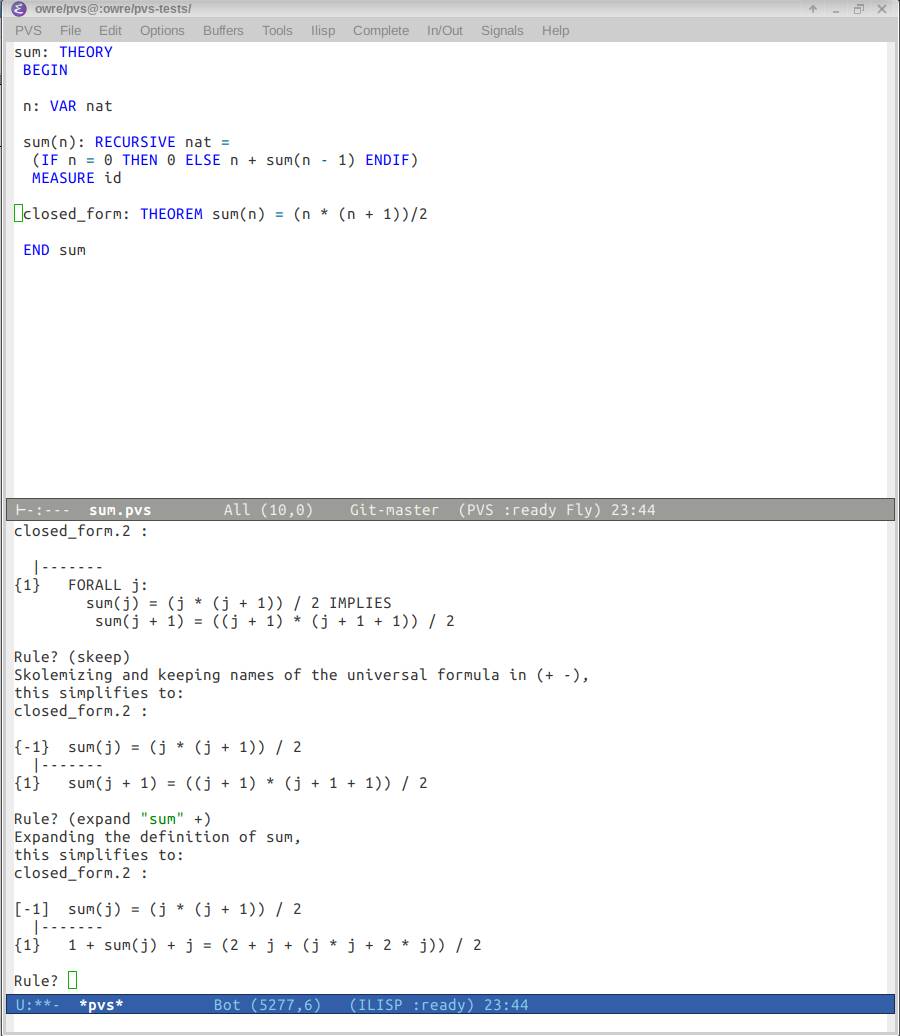
\includegraphics[width=\textwidth]{pvs-screen1.png}
\caption{The \texttt{sum} Specification in Emacs}\label{sum-screen}
\end{figure}

This simple theory has no parameters and contains three declarations.  The
first declares \texttt{n} to be a variable of type \texttt{nat}, the
built-in type of natural numbers.  The next declaration is a recursive
definition of the function \texttt{sum(n)} whose value is the sum of the
first \texttt{n} natural numbers.  Associated with this definition is a
\emph{measure} function, following the \texttt{MEASURE} keyword, which is
explained below.  The final declaration is a formula which gives the
closed form of the sum.

The \texttt{sum} theory may be introduced to the system in a number of
ways, all of which create a file with a \texttt{.pvs}
extension.\footnote{The file does not have to be named \texttt{sum.pvs}, it
simply needs the \texttt{.pvs} extension.}  The most common ways are:
\begin{enumerate}

\item Simply use \texttt{M-x find-file} (\key{C-x C-f}), or \texttt{M-x
find-pvs-file} (\ecmd{ff}, \key{C-c C-f}), provide \texttt{sum.pvs} for
the file name and type in the specification.\footnote{If there is already
a file called \texttt{sum.pvs} in the current context, this will load that
file.}

\item Use the \texttt{M-x new-pvs-file} command (\ecmd{nf}) to create a
new PVS file, and type \texttt{sum} when prompted for a file name.  Then
simply type the specification into the buffer (a basic template will be provided). 

\item Since the file is included in the distribution in the
\texttt{Examples} subdirectory of the main PVS directory, it can be
imported with the \texttt{M-x import-pvs-file} command (\ecmd{imf}).  Use
the \ecmd{whereis-pvs} command to find the path of the main PVS directory.

\item Finally, any external means of introducing a file with extension
\texttt{.pvs} into the current directory will make it available to the
system; for example, going to a \unix\ window and using \texttt{vi} to
type it in, or \texttt{cp} to copy it from the \texttt{Examples}
subdirectory.

\end{enumerate}

\section{Parsing and Typechecking}

Once the \texttt{sum} specification is displayed in the current buffer, it
can be parsed with the \iecmd{parse} (\ecmd{pa}) command, which checks the
syntactic consistency of the specification and creates the internal
abstract representation for the theory described by the specification.  If
the system finds an error during parsing, an error window will pop up with
an error message, and the cursor will be placed in the vicinity of the
error.  If you didn't get an error, introduce one (say by misspelling the
\texttt{VAR} keyword), then move the cursor somewhere else and parse the
file again---note that the buffer is automatically saved.  Fix the error
and parse once more.  In practice, the parse command is rarely used, as
the system automatically parses the specification when it needs to.

\index{typecheck|(}

The next step is to typecheck the file by typing \iecmd{typecheck}
(\iecmd{tc}, \key{C-c C-t}), which checks for semantic errors, such as
undeclared names and ambiguous types.  After \texttt{sum} has been
typechecked, a message is displayed in the minibuffer indicating that two
\tccs\index{TCCs@\tccs|(} were generated.  These \tccs\ represent
\emph{proof obligations}\index{proof obligations} that must be discharged
before the \texttt{sum} theory can be considered typechecked.  The proofs
of the \tccs\ may be postponed indefinitely, though in general it is a
good idea to view \tccs\ to convince yourself that they are provable
before moving on to other proofs in your specification.  \tccs\ can be
viewed using the \iecmd{show-tccs} (\iecmd{tccs}, \key{C-c C-q s})
command, the results of which are shown in Figure~\ref{sum-tccs} below.

\pvstheory{sum-tccs}{\tccs\ for Theory \texttt{sum}}{sum-tccs}

The first \tcc\ is due to the fact that \texttt{sum} takes an argument of
type \texttt{nat}, but the type of the argument in the recursive call to
\texttt{sum} is integer, since \texttt{nat} is not closed under subtraction.
Note that the \tcc\ includes the condition \texttt{NOT n = 0}, which holds
in the branch of the \texttt{IF-THEN-ELSE} in which the expression
\texttt{n - 1} occurs.

The second \tcc\ is needed to ensure that the function \texttt{sum} is
total, \ie\ terminates.  PVS does not directly support partial functions,
although its powerful subtyping mechanism allows PVS to express many
operations that are traditionally regarded as partial.  The measure
function is used to show that recursive definitions are total by requiring
the measure to decrease with each recursive call.

These \tccs\ are trivial, and in fact can be discharged automatically by
using the \ecmd{typecheck-prove} (\ecmd{tcp}) command, which attempts to
prove all \tccs\ that have been generated.  (Try it.)
\index{TCCs@\tccs|)}\index{typecheck|)}

\section{Proving}

We are now ready to try to prove the main theorem.  Place the cursor on
the line containing the \texttt{closed\_form} theorem, and type
\iecmd{prove} (\iecmd{pr} or \key{C-c p}).  A new buffer will pop up, the
formula will be displayed, and the cursor will appear at the
\texttt{Rule?}  prompt, indicating that the prover is ready to accept
input.  The commands needed to prove this theorem constitute only a very
small subset of the commands available to the prover.  In fact, for this
proof all that is actually needed is the single command
\texttt{(induct-and-simplify "n")}, which is a more powerful strategy.
For more information on these and other prover commands consult the prover
guide~\cite{PVS:prover}.

First, notice the display, which consists of a single formula (labeled
\texttt{\{1\}}) under a dashed line.  This is a
\emph{sequent}\index{sequent}; formulas above the dashed lines are called
\emph{antecedents}\index{antecedent} and those below are called
\emph{consequents}\index{consequent}.  The interpretation of a sequent is
that the conjunction of the antecedents implies the disjunction of the
consequents.  Either or both of the antecedents and consequents may be
empty.  An empty antecedent is equivalent to \texttt{true}, and an empty
consequent is equivalent to \texttt{false}, so if both are empty the
sequent is \texttt{false}.  Every proof in PVS starts with a single
consequent.

The basic objective of the proof is to generate a \emph{proof
tree}\index{proof tree} of sequents in which all of the leaves are
trivially true.  The nodes of the proof tree are sequents, and while in
the prover you will always be looking at an unproved leaf of the tree,
called the \emph{current} sequent.\index{current sequent} The
\emph{current} branch\index{current branch} of a proof is the branch
leading back to the root from the current sequent.  When a given branch is
complete (\ie\ ends in a proved leaf), the prover automatically moves on
to the next unproved branch, or, if there are no more unproven branches,
notifies you that the proof is complete.

Now on to the proof.  We will prove this formula by induction on
\texttt{n}.  To do this, type \texttt{(induct "n")}\index{prover
commands!induct@\texttt{induct}}.\footnote{PVS expressions are
case-sensitive, and must be put in double quotes when they appear as
arguments in prover commands.} This is not an Emacs command, rather it
is typed directly at the prompt, including the parentheses.  As indicated,
two subgoals are generated; the one displayed is the base case, where
\texttt{n} is \texttt{0}.  To see the inductive step, type
\texttt{(postpone)}\index{prover commands!postpone@\texttt{postpone}},
which postpones the current subgoal and moves on to the next unproved one.
Type \texttt{(postpone)} a second time to cycle back to the original
subgoal (labeled \texttt{closed\_form.1}).

Three extremely useful Emacs key bindings to know here are \key{M-p},
\key{M-n}, and \key{M-s}.  \key{M-p} gets the last input typed to the
prover; further uses of \key{M-p} cycle back in the input history.
\key{M-n} works in the opposite direction.  To use \key{M-s}, type the
beginning of a command that was previously input, and type \key{M-s}.
This will get the previous input that matches the partial input; further
uses of \key{M-s} will find earlier matches.  Try these key bindings out;
they are easier to use than to explain.  Thus to type the second postpone
command above, you can either type \key{M-p} or type \texttt{(po} followed
by \key{M-s}.  Section~\ref{prover-emacs} on page~\pageref{prover-emacs}
describes further useful shortcut commands for the prover.

To prove the base case, we need to expand the definition of \texttt{sum},
which is done by typing \texttt{(expand "sum")}\index{prover
commands!expand@\texttt{expand}}.  After expanding the definition of
\texttt{sum}, we issue the \texttt{(assert)}\index{prover
commands!assert@\texttt{assert}} command, which applies the decision
procedures of the prover to simplify the consequent to \texttt{TRUE},
completing the proof of this subgoal.  The prover then automatically moves
on to the next subgoal, which is the inductive step.

The first thing to do here is to eliminate the \texttt{FORALL} quantifier.
This can most easily be done with the \texttt{skolem!}\ \index{prover
commands!skolem@\texttt{skolem"!}}  command\footnote{The exclamation point
differentiates this command from the \texttt{skolem} command, where you
provide the new constant names.}, which provides new constants for the
bound variables.  To invoke this command type \texttt{(skolem!)} at the
prompt.  The resulting formula may be simplified by typing
\texttt{(flatten)}\index{prover commands!flatten@\texttt{flatten}}, which
will break up the consequent into a new antecedent and consequent.  The
obvious thing to do now is to expand the definition of \texttt{sum} in the
consequent.  This again is done with the \texttt{expand} command, but this
time we want to control where it is expanded, as expanding it in the
antecedent will not help.  So we type \texttt{(expand "sum" +)},
indicating that we want to expand \texttt{sum} in the
consequent.\footnote{We could also have specified the exact formula number
(here \texttt{1}), but including formula numbers in a proof tends to make
it less robust in the face of changes.  There is more discussion of this
in the prover guide~\cite{PVS:prover}.}

The final step is to invoke the PVS decision procedures, which can
automatically decide certain fragments of arithmetic.  This is done by
typing \texttt{(assert)}. The \texttt{assert}\index{prover
commands!assert@\texttt{assert}} command actually does a lot more than
decide arithmetical formulas, performing three basic tasks:
\begin{itemize}\def\itemsep{0in}
\item It tries to prove the subgoal using the decision procedures.

\item It stores the subgoal information in an underlying database,
allowing automatic use to be made of it later.

\item It simplifies the subgoal by rewriting (if any auto-rewrites have
been given) and by using the underlying decision procedures.
\end{itemize}
These arithmetic and equality procedures are the main workhorses of most
PVS proofs.

The proof is now complete, and is saved in the \texttt{sum.prf} file.  The
buffer from which the \cmd{prove} command was issued is then redisplayed
if necessary, and the cursor is placed on the formula that was just
proved.  The entire proof transcript is shown below.  Yours may be
slightly different, depending on your window size and the timings involved.

{\smaller\smaller
\begin{alltt}
  closed_form :  

    |-------
  \{1\}   FORALL (n: nat): sum(n) = n * (n + 1) / 2

  Rule? (induct "n")
  Inducting on n on formula 1,
  this yields  2 subgoals: 
  closed_form.1 :  

    |-------
  \{1\}   sum(0) = 0 * (0 + 1) / 2

  Rule? (postpone)
  Postponing closed_form.1.

  closed_form.2 :  

    |-------
  \{1\}   FORALL (j: nat):
          sum(j) = j * (j + 1) / 2 IMPLIES sum(j + 1) = (j + 1) * (j + 1 + 1) / 2

  Rule? (postpone)
  Postponing closed_form.2.

  closed_form.1 :  

    |-------
  \{1\}   sum(0) = 0 * (0 + 1) / 2

  Rule? (expand "sum")
  Expanding the definition of sum,
  this simplifies to: 
  closed_form.1 :  

    |-------
  \{1\}   0 = 0 / 2

  Rule? (assert)
  Simplifying, rewriting, and recording with decision procedures,

  This completes the proof of closed_form.1.

  closed_form.2 :  

    |-------
  \{1\}   FORALL (j: nat):
          sum(j) = j * (j + 1) / 2 IMPLIES sum(j + 1) = (j + 1) * (j + 1 + 1) / 2

  Rule? (skolem!)
  Skolemizing,
  this simplifies to: 
  closed_form.2 :  

    |-------
  \{1\}   sum(j!1) = j!1 * (j!1 + 1) / 2 IMPLIES
         sum(j!1 + 1) = (j!1 + 1) * (j!1 + 1 + 1) / 2

  Rule? (flatten)
  Applying disjunctive simplification to flatten sequent,
  this simplifies to: 
  closed_form.2 :  

  \{-1\}  sum(j!1) = j!1 * (j!1 + 1) / 2
    |-------
  \{1\}   sum(j!1 + 1) = (j!1 + 1) * (j!1 + 1 + 1) / 2

  Rule? (expand "sum" +)
  Expanding the definition of sum,
  this simplifies to: 
  closed_form.2 :  

  [-1]  sum(j!1) = j!1 * (j!1 + 1) / 2
    |-------
  \{1\}   1 + sum(j!1) + j!1 = (2 + j!1 + (j!1 * j!1 + 2 * j!1)) / 2

  Rule? (assert)
  Simplifying, rewriting, and recording with decision procedures,

  This completes the proof of closed_form.2.

  Q.E.D.


  Run time  = 0.81 secs.
  Real time = 223.01 secs.

\end{alltt}}

A brief version of the just completed proof can be generated by the command
command \iecmd{show-last-proof}.

\section{Status}

Now type \iecmd{status-proof-theory} (\iecmd{spt}) and you will see a
buffer that displays the three formulas in \texttt{sum}, along with an
indication of their proof status.  This command is useful to see which
formulas and \tccs\ still require proofs.  Another useful command is
\iecmd{status-proofchain} (\ecmd{spc}), which analyzes a given proof to
determine its dependencies.  To use this, go to the \texttt{sum.pvs}
buffer, place the cursor on the \texttt{closed\_form} theorem, and enter
the command.  A buffer will pop up indicating that the proof is
complete, and that it depends on the \tccs\ and the \texttt{nat\_induction}
axiom, as well as some definitions and \tccs\ provided by the prelude.

\section{Generating \LaTeX}

In order to try out this section, you must have access to \LaTeX\
\index{LaTeX@\LaTeX} and a \TeX\ previewer such as
\texttt{xdvi}\index{xdvi}.

Type \iecmd{latex-theory-view} (\iecmd{ltv}).  You will be prompted for
the theory name to which you should type \texttt{sum}, or just
\texttt{Return} if \texttt{sum} is the default.  You will then be prompted
for the \TeX\ previewer name.  Either the previewer must be in your path,
or the entire pathname must be given.  This information will only be
prompted for once per session, after which PVS assumes that you want to
use the same previewer.  You can set the previewer automatically,
by adding the following line to your \texttt{\char'176/.pvsemacs} file.
{\small
\begin{alltt}
\hspace*{2em}  (setq pvs-latex-viewer "\textit{previewer}")
\end{alltt}}

\begin{figure}[ht]
\begin{center}
\begin{boxedminipage}{\textwidth}
{\small\small\input{sum-nosub}}
\end{boxedminipage}
\end{center}
\caption{Theory \texttt{sum} with default translations}\label{sum-plain}
\end{figure}

After a few moments the previewer will pop up displaying the \texttt{sum}
theory, as shown in Figure~\ref{sum-plain}.  Note that \texttt{*} has been
translated as $\times$ and \texttt{LAMBDA} as $\lambda$.  These and other
translations are built into PVS; you may also specify translations for
keywords and identifiers by providing a substitution file named
\texttt{pvs-tex.sub}, that contains commands to customize the \LaTeX\
output.  For example, if the substitution file contains the two lines
{\small\small
\begin{alltt}
    THEORY key 7 \verb|{\large\textbf{\textrm{Theory}}}|
    sum    1   2 \verb|{\sum_{i = 0}^{#1} i}|
\end{alltt}}
\noindent the output will look like Figure~\ref{sum-sub}.  See
Section~\ref{latex-output} on page~\pageref{latex-output} for more
details.

\begin{figure}[t]
\begin{boxedminipage}{\textwidth}
{\small\small% The following substitutions are from the file:
%   /home/owre/pvs.git/pvs-tex.sub
\def\munderscoretimestwofn#1#2{{#1 \times #2}}% How to print function m_times with arity (2)
\def\fmunderscoretimestwofn#1#2{{#1 \times #2}}% How to print function fm_times with arity (2)
\def\sigmaunderscoretimestwofn#1#2{{#1 \times #2}}% How to print function sigma_times with arity (2)
\def\generatedunderscoresubsetunderscorealgebraonefn#1{{{\cal A}(#1)}}% How to print function generated_subset_algebra with arity (1)
\def\generatedunderscoresigmaunderscorealgebraonefn#1{{{\cal S}(#1)}}% How to print function generated_sigma_algebra with arity (1)
\def\aeunderscoredecreasingotheronefn#1{{\pvsid{decreasing?}(#1)~\mbox{\it a.e.}}}% How to print function ae_decreasing? with arity (1)
\def\aeunderscoreincreasingotheronefn#1{{\pvsid{increasing?}(#1)~\mbox{\it a.e.}}}% How to print function ae_increasing? with arity (1)
\def\aeunderscoreconvergenceothertwofn#1#2{{#1 \longrightarrow #2~\mbox{\it a.e.}}}% How to print function ae_convergence? with arity (2)
\def\aeunderscoreeqothertwofn#1#2{{#1 = #2~\mbox{\it a.e.}}}% How to print function ae_eq? with arity (2)
\def\aeunderscoreleothertwofn#1#2{{#1 \leq #2~\mbox{\it a.e.}}}% How to print function ae_le? with arity (2)
\def\aeunderscoreposotheronefn#1{{#1> 0~\mbox{\it a.e.}}}% How to print function ae_pos? with arity (1)
\def\aeunderscorenonnegotheronefn#1{{#1 \geq 0~\mbox{\it a.e.}}}% How to print function ae_nonneg? with arity (1)
\def\aeunderscorezerootheronefn#1{{#1 = 0~\mbox{\it a.e.}}}% How to print function ae_0? with arity (1)
\def\xunderscorelttwofn#1#2{{#1 < #2}}% How to print function x_lt with arity (2)
\def\xunderscoreletwofn#1#2{{#1 \leq #2}}% How to print function x_le with arity (2)
\def\xunderscoreeqtwofn#1#2{{#1 = #2}}% How to print function x_eq with arity (2)
\def\xunderscoretimestwofn#1#2{{#1 \times #2}}% How to print function x_times with arity (2)
\def\xunderscoreaddtwofn#1#2{{#1 + #2}}% How to print function x_add with arity (2)
\def\xunderscorelimitonefn#1{{\pvsid{limit}(#1)}}% How to print function x_limit with arity (1)
\def\xunderscoresumonefn#1{{\sum #1}}% How to print function x_sum with arity (1)
\def\xunderscoresigmathreefn#1#2#3{{\sum_{#1}^{#2} #3}}% How to print function x_sigma with arity (3)
\def\xunderscoresuponefn#1{{\pvsid{sup}(#1)}}% How to print function x_sup with arity (1)
\def\xunderscoreinfonefn#1{{\pvsid{inf}(#1)}}% How to print function x_inf with arity (1)
\def\pointwiseunderscoreconvergesunderscoredowntoothertwofn#1#2{{#1 \searrow #2}}% How to print function pointwise_converges_downto? with arity (2)
\def\pointwiseunderscoreconvergesunderscoreuptoothertwofn#1#2{{#1 \nearrow #2}}% How to print function pointwise_converges_upto? with arity (2)
\def\pointwiseunderscoreconvergenceothertwofn#1#2{{#1 \longrightarrow #2}}% How to print function pointwise_convergence? with arity (2)
\def\convergesunderscoredowntoothertwofn#1#2{{#1 \searrow #2}}% How to print function converges_downto? with arity (2)
\def\convergesunderscoreuptoothertwofn#1#2{{#1 \nearrow #2}}% How to print function converges_upto? with arity (2)
\def\convergenceothertwofn#1#2{{#1 \longrightarrow #2}}% How to print function convergence? with arity (2)
\def\convergencetwofn#1#2{{#1 \longrightarrow #2}}% How to print function convergence with arity (2)
\def\crossunderscoreproducttwofn#1#2{{#1 \times #2}}% How to print function cross_product with arity (2)
\def\conjugateonefn#1{{\overline{#1}}}% How to print function conjugate with arity (1)
\def\cunderscoredivtwofn#1#2{{#1/#2}}% How to print function c_div with arity (2)
\def\cunderscoremultwofn#1#2{{#1\times#2}}% How to print function c_mul with arity (2)
\def\cunderscoresubtwofn#1#2{{#1-#2}}% How to print function c_sub with arity (2)
\def\cunderscorenegonefn#1{{-#1}}% How to print function c_neg with arity (1)
\def\cunderscoreaddtwofn#1#2{{#1+#2}}% How to print function c_add with arity (2)
\def\Imonefn#1{{\Im(#1)}}% How to print function Im with arity (1)
\def\Reonefn#1{{\Re(#1)}}% How to print function Re with arity (1)
\def\Etwofn#1#2{{\mathbb{E}(#1~|~#2)}}% How to print function E with arity (2)
\def\Eonefn#1{{\mathbb{E}(#1)}}% How to print function E with arity (1)
\def\Ptwofn#1#2{{\mathbb{P}(#1~|~#2)}}% How to print function P with arity (2)
\def\Ponefn#1{{\mathbb{P}(#1)}}% How to print function P with arity (1)
\def\xtwofn#1#2{{#1\times#2}}% How to print function x with arity (2)
\def\asttwofn#1#2{{#1\ast#2}}% How to print function ast with arity (2)
\def\minusonefn#1{{{#1}^{-}}}% How to print function minus with arity (1)
\def\plusonefn#1{{{#1}^{+}}}% How to print function plus with arity (1)
\def\astonefn#1{{{#1}^{\ast}}}% How to print function ast with arity (1)
\def\dottwofn#1#2{{#1\bullet#2}}% How to print function dot with arity (2)
\def\integralthreefn#1#2#3{{\int_{#1}^{#2} #3}}% How to print function integral with arity (3)
\def\integraltwofn#1#2{{\int_{#1} #2}}% How to print function integral with arity (2)
\def\integralonefn#1{{\int#1}}% How to print function integral with arity (1)
\def\normonefn#1{{\left||{#1}\right||}}% How to print function norm with arity (1)
\def\phionefn#1{{\pvssubscript{\phi}{#1}}}% How to print function phi with arity (1)
\def\infunderscoreclosedonefn#1{{\left(-\infty,~#1\right]}}% How to print function inf_closed with arity (1)
\def\closedunderscoreinfonefn#1{{\left[#1,~\infty\right)}}% How to print function closed_inf with arity (1)
\def\infunderscoreopenonefn#1{(-\infty,~#1)}% How to print function inf_open with arity (1)
\def\openunderscoreinfonefn#1{(#1,~\infty)}% How to print function open_inf with arity (1)
\def\closedtwofn#1#2{{\left[#1,~#2\right]}}% How to print function closed with arity (2)
\def\opentwofn#1#2{(#1,~#2)}% How to print function open with arity (2)
\def\sigmathreefn#1#2#3{{\sum_{#1}^{#2} #3}}% How to print function sigma with arity (3)
\def\sigmatwofn#1#2{{\sum_{#1} {#2}}}% How to print function sigma with arity (2)
\def\ceilingonefn#1{{\lceil{#1}\rceil}}% How to print function ceiling with arity (1)
\def\flooronefn#1{{\lfloor{#1}\rfloor}}% How to print function floor with arity (1)
\def\absonefn#1{{\left|{#1}\right|}}% How to print function abs with arity (1)
\def\roottwofn#1#2{{\sqrt[#2]{#1}}}% How to print function root with arity (2)
\def\sqrtonefn#1{{\sqrt{#1}}}% How to print function sqrt with arity (1)
\def\sqonefn#1{{\pvssuperscript{#1}{2}}}% How to print function sq with arity (1)
\def\expttwofn#1#2{{\pvssuperscript{#1}{#2}}}% How to print function expt with arity (2)
\def\opcarettwofn#1#2{{\pvssuperscript{#1}{#2}}}% How to print function ^ with arity (2)
\def\indexedunderscoresetsotherIIntersectiononefn#1{{\bigcap #1}}% How to print function indexed_sets.IIntersection with arity (1)
\def\indexedunderscoresetsotherIUniononefn#1{{\bigcup #1}}% How to print function indexed_sets.IUnion with arity (1)
\def\setsotherIntersectiononefn#1{{\bigcap #1}}% How to print function sets.Intersection with arity (1)
\def\setsotherUniononefn#1{{\bigcup #1}}% How to print function sets.Union with arity (1)
\def\setsotherremovetwofn#1#2{{(#2 \setminus \{#1\})}}% How to print function sets.remove with arity (2)
\def\setsotheraddtwofn#1#2{{(#2 \cup \{#1\})}}% How to print function sets.add with arity (2)
\def\setsotherdifferencetwofn#1#2{{(#1 \setminus #2)}}% How to print function sets.difference with arity (2)
\def\setsothercomplementonefn#1{{\overline{#1}}}% How to print function sets.complement with arity (1)
\def\setsotherintersectiontwofn#1#2{{(#1 \cap #2)}}% How to print function sets.intersection with arity (2)
\def\setsotheruniontwofn#1#2{{(#1 \cup #2)}}% How to print function sets.union with arity (2)
\def\setsotherstrictunderscoresubsetothertwofn#1#2{{(#1 \subset #2)}}% How to print function sets.strict_subset? with arity (2)
\def\setsothersubsetothertwofn#1#2{{(#1 \subseteq #2)}}% How to print function sets.subset? with arity (2)
\def\setsothermembertwofn#1#2{{(#1 \in #2)}}% How to print function sets.member with arity (2)
\def\opohtwofn#1#2{{#1\circ#2}}% How to print function O with arity (2)
\def\opdividetwofn#1#2{{\frac{#1}{#2}}}% How to print function / with arity (2)
\def\optimestwofn#1#2{{#1\times#2}}% How to print function * with arity (2)
\def\opdifferenceonefn#1{{-#1}}% How to print function - with arity (1)
\def\opdifferencetwofn#1#2{{#1-#2}}% How to print function - with arity (2)
\def\opplustwofn#1#2{{#1+#2}}% How to print function + with arity (2)
% The following substitutions are from the file:
%   /home/owre/pvs.git/doc/wift95/pvs-tex.sub
\def\sumonefn#1{{\sum_{i = 0}^{#1} i}}% How to print function sum with arity (1)
\begin{alltt}
\pvsid{sum}: \({\large\bf Theory}\)
 \pvskey{BEGIN}

  \(n\): \pvskey{VAR} \(\mathbb{N}\)\vspace*{\pvsdeclspacing}

  \(\sumonefn{n}\): \pvskey{RECURSIVE} \(\mathbb{N}\) \pvskey{=} \pvsid{(}\pvskey{IF} \(n\) \(=\) \(0\) \pvskey{THEN} \(0\) \pvskey{ELSE} \(\opplustwofn{n}{\sumonefn{\opdifferencetwofn{n}{1}}}\) \pvskey{ENDIF}\pvsid{)}
     \pvskey{MEASURE} \pvsid{(}\(\lambda\) \(n\): \(n\)\pvsid{)}\vspace*{\pvsdeclspacing}

  \pvsid{closed\_form}: \pvskey{THEOREM} \(\sumonefn{n}\) \(=\) \(\opdividetwofn{\pvsid{(}\optimestwofn{n}{\pvsid{(}\opplustwofn{n}{1}\pvsid{)}}\pvsid{)}}{2}\)\vspace*{\pvsdeclspacing}

 \pvskey{END} \pvsid{sum}\end{alltt}
}
\end{boxedminipage}
\caption{Theory \texttt{sum} with additional translations}\label{sum-sub}
\end{figure}

\vspace*{1in}

\setcounter{footnote}{0}
% Document Type: LaTeX
% Master File: user-guide.tex
\chapter{PVS Commands}
\label{commands}
\setcounter{footnote}{0}

This chapter contains descriptions for all PVS commands; the commands are
grouped according to function.  A summary of the information in this
chapter is also provided in the buffer displayed by the \ecmd{pvs-help}
command.  The information in this chapter is best absorbed after reading
and experimenting with the brief tour provided in
Chapter~\ref{system-tutorial}.

Each of the following sections begins with a table summarizing the
commands discussed in that section; each table entry gives the full name
of the command, available aliases and/or key bindings, a brief
description, and the effect of providing command arguments.  Commands are
invoked by typing \texttt{M-x} followed by the command name or its
abbreviation, or by using a (less mnemonic) key sequence.  For example,
the \cmd{typecheck} command can be invoked by typing \ecmd{typecheck} or
one of the alternate forms \ecmd{tc} or \key{C-c C-t}.  The behavior of many
of the commands can be modified by providing an argument, and many of the
commands work on regions.\footnote{See Section 4.9 of~\cite{emacs20} for
details on providing arguments to commands, and Section 9 for creating and
manipulating regions.} For example, preceding the \cmd{typecheck} command
with a \key{C-u} or \key{M-1} forces the file to be reparsed and
typechecked, even if it has already been typechecked.  Each command that
takes an argument has a second line prefixed by \emph{Arg:} that
describes the effect of the argument.

Many PVS commands are appropriate at either the file or theory level;
yielding two different commands.  For example, the command for
creating a new PVS file is \cmd{new-pvs-file}, while the command
\cmd{new-theory} creates a template for a new theory within the current
PVS file.  In general, a command \emph{foo} that applies to both
files and theories will have a version named \ecmd{\textit{foo}-pvs-file}
and one named \ecmd{\textit{foo}-theory}.

\section{Exiting PVS}

\begin{pvscmds}
\icmd{exit-pvs} & \key{C-x C-c} & Terminate PVS session \\
\icmd{suspend-pvs} & \key{C-x C-z} & Suspend PVS \\
\end{pvscmds}

The \cmd{exit-pvs} command first saves the context information (see the
\icmd{save-context} command) and then exits PVS\@.  If there is a proof in
progress, the system will not exit, but will instead output a message
asking you to exit the prover, thus giving you the opportunity to save the
proof before exiting.

The \cmd{suspend-pvs} command suspends the Emacs process, except under
X-windows, where the command has no effect.  The system first asks whether
the context should be saved; if you answer \texttt{yes} the
\icmd{save-context} command is invoked prior to suspending PVS.  This may
take a while, as the \cmd{save-context} may have to save any number of
files, depending on what has changed in the context.  The suspended job
can be restarted from the \unix\ shell in which it was suspended by first
determining the job number (using the \unix\ command ``\texttt{jobs}'')
and then typing ``\texttt{fg \%$n$}'', where $n$ is the job
number.\footnote{This assumes you are running the \texttt{csh} or
\texttt{tcsh} shell. To restart under a shell lacking job control, use the
\unix\ command \texttt{ps} to determine the process id ($pid$) and then do
\texttt{kill -CONT pid}.}

\section{Getting Help}
\begin{pvscmds}
\icmd{help-pvs}, \icmd{pvs-help} & \key{C-c h} & Display the PVS help
  buffer \\
\icmd{help-pvs-bnf}, \icmd{pvs-help-bnf} & \key{C-c C-h b} & Display the
  pvs grammar \\
\icmd{help-pvs-language}, & \key{C-c C-h l} & Display help for the PVS
  language \\
\quad\icmd{pvs-help-language} & & \\
\icmd{help-pvs-prover}, & \key{C-c C-h p} & Display help for the prover
  commands \\
\quad\icmd{pvs-help-prover} & & \\
\icmd{help-pvs-prover-command}, & \key{C-c C-h c} &
  Display help for prover command \\
\quad\icmd{pvs-help-prover-command} & & \\
\icmd{help-pvs-prover-strategy}, & \key{C-c C-h s} &
  Displays the specified prover strategy \\
\quad\icmd{pvs-help-prover-strategy} & & \\
\icmd{x-prover-commands} & & Displays the prover commands in a \\
& & \quad Tcl/Tk window \\
\icmd{help-pvs-prover-emacs}, & \key{C-c C-h e} &
  Display help for prover emacs commands \\
\quad\icmd{pvs-help-prover-emacs} & & \\
\icmd{pvs-release-notes}, & \key{C-c C-h r} & Display PVS release notes \\
\end{pvscmds}

The \cmd{help-pvs} command displays a summary of PVS commands in the
\ibuf{PVS Help} buffer.  Help may be obtained for an individual command by
typing \texttt{C-h f} followed by the command or its abbreviation, or by
typing \texttt{C-h k} followed by the key sequence that invokes the
command.  These are built in to Emacs, and may be used to get help for
any Emacs command or key sequence, not just PVS commands.

The \cmd{help-pvs-bnf} command provides the PVS grammar in BNF form, and
the \cmd{help-pvs-language} command displays a summary of the PVS language
with examples in the \ibuf{Language Help} buffer.

The \cmd{help-pvs-prover} command displays the documentation string for
all of the prover commands in the \ibuf{Prover Help} buffer.  The
\cmd{help-pvs-prover-command} displays the documentation string for the
specified command, and the \cmd{help-pvs-prover-strategy} command provides
the arguments, definition, format string, and documentation string for the
specified command.  The latter is useful for finding out exactly what a
strategy does, or for defining your own strategies based on existing ones.
If you are running under the X window system, \icmd{x-prover-commands}
provides an easy interface to get help for individual prover commands.

The \cmd{help-pvs-prover-emacs} command displays a summary of the commands
that provide a convenient Emacs interface to the PVS prover.  This is
discussed in more detail in Section~\ref{prover-emacs},
page~\pageref{prover-emacs}.  The help text appears in the \ibuf{Prover
Emacs Help} buffer.

The \cmd{pvs-release-notes} command displays the release notes for the
running version of PVS.  The text appears in the \ibuf{PVS Release Notes}
buffer.

\section{Editing PVS Files}

\begin{pvscmds}
\icmd{forward-theory} & \key{M-\char125} & Move forward to beginning of next theory \\
\icmd{backward-theory} & \key{M-\char123} & Move backward to beginning of previous theory \\
\icmd{find-unbalanced-pvs} & \key{C-c ]} & Find unbalanced delimiters \\
\icmd{comment-region} & \key{C-c ;} & Comment out all lines in the current region \\
 & & \emph{Arg:} Uncomment all lines in the current region\\
\end{pvscmds}

PVS specification files are edited using the standard Emacs editing
commands.  Appendix~\ref{emacs-intro}, page~\pageref{emacs-intro} gives a
brief introduction to the most useful Emacs commands for editing PVS
files.

The \cmd{forward-theory} and \cmd{backward-theory} commands are used to
move to different theories within a single PVS file.  The cursor is
moved to the beginning of a theory; if there are no preceding or
following theories to move to, the message ``\texttt{No more theories}''
or ``\texttt{No earlier theories}'' is displayed and the cursor remains unchanged.

The \cmd{find-unbalanced-pvs} command checks whether there are any
unbalanced parentheses (\texttt{( )}), square brackets (\texttt{[ ]}), curly
braces (\verb|{ }|), or \texttt{BEGIN-END} pairs.  If none are found, the
message ``\texttt{All delimiters balance}'' is displayed.  Otherwise the
cursor is left at the token for which there is no match and a
corresponding message is displayed.

The \cmd{comment-region} command inserts the comment character
(\texttt{\%}) at the beginning of every line in the specified region.  To
uncomment a region, simply provide an argument to the command, and all
commented lines within the region will be uncommented.

\section{Parsing and Typechecking}

\subsection{Parsing}

\begin{pvscmds}
\icmd{parse} & \icmd{pa} & Parse file in current buffer \\
             & & \emph{Arg:} Forces the file to be reparsed \\
\end{pvscmds}

Parsing a PVS specification accomplishes two things: first, it checks that
the specification is syntactically correct, \ie\ satisfies the PVS
grammar, and second, it builds the internal abstract grammar data
structures.  The \cmd{parse} command is not normally used, as typechecking
will automatically parse the file if required.  Note that only files (with
extension \texttt{.pvs}) may be parsed.  When a file is parsed, it becomes a
part of the context if it wasn't already, and any proofs that have been
saved for the file are reinstated.  If the file being parsed has a valid
\texttt{.bin} file, then this file is loaded instead (this will result in
the file being typechecked as well as parsed).

Parsing is invoked by moving the cursor to a buffer containing a file in
the current context, and issuing the \cmd{parse} command.  While parsing
the file, the minibuffer displays the message ``\texttt{Parsing
\textit{foo}}.''  If there is no error, the message ``\texttt{\textit{foo}
parsed in \textit{\#} seconds}'' is displayed.  If the file has not changed
since the last time it was parsed, the message ``\texttt{\textit{foo} is
already parsed}'' is displayed.  To force reparsing, provide an argument
to the parse command.  Note that the argument is usually not needed, as
changes to the file are automatically detected by the system and the file
is reparsed in that case.

When an error is detected, the file is displayed with the cursor at the
location where the error was detected, which is frequently after the
actual source of the error.  In addition, the \ibuf{PVS Error} buffer is
displayed with an explanatory error message.  You may need to consult the
language manual for details on the grammar.

Certain language features may result in the parser producing theory
messages.  See the \cmd{show-theory-messages} command
(page~\pageref{tc-info}) for details.


\subsection{Typechecking}

\begin{pvscmds}
\icmd{typecheck} & \icmd{tc}, \key{C-c C-t} & Typecheck theories in current buffer \\
& & \emph{Arg:} Force reparsing and retypechecking \\
\icmd{typecheck-importchain} & \icmd{tci} & Typecheck importchain of theories \\
& & \emph{Arg:} Force reparsing and retypechecking \\
\icmd{typecheck-prove} & \icmd{tcp} & Typecheck theories, proving \tccs \\
& & \emph{Arg:} Force reparsing and retypechecking \\
\icmd{typecheck-prove-importchain} & \icmd{tcpi} & Typecheck importchain
of theories,\\ & &  proving \tccs \\
& & \emph{Arg:} Force reparsing and retypechecking \\
\end{pvscmds}

Typechecking a PVS specification checks semantic constraints, determines
the types of expressions, and resolves names (see the language
manual~\cite{PVS:language}).  Typechecking\cmdindex{typecheck} is invoked
much like parsing, and automatically parses the file if necessary.  Errors
are indicated in the same manner as for parsing, although the cursor is
usually more accurately positioned at the error.  As in parsing, an
argument to the command forces reparsing and retypechecking.  Without the
argument, \cmd{typecheck} and \cmd{typecheck-importchain} are the same.
With the argument, \cmd{typecheck} only reparses and retypechecks the
current file, while \cmd{typecheck-importchain} forces reparsing and
retypechecking of the entire import chain of the theories of the current
file.

Forcing a file to be retypechecked is done primarily for development and
debugging, as is the case for reparsing.  If you have typechecked a set of
PVS files, made some changes and found an error on retypechecking that
shouldn't have occurred, try forcing a typecheck of the file where the
error occurred.  If that doesn't help, try forcing with
\cmd{typecheck-importchain}.  The error should disappear after that,
unless it is a true typecheck error.  If it is not a simple typecheck
error, send a bug report to \texttt{pvs-bugs@csl.sri.com}.

The typechecker will attempt to typecheck any theories
appearing in \texttt{IMPORTING} clauses.  If the theories appear in the
current context, then the associated file is typechecked, otherwise
PVS tries to find a file with the same name as the theory.  For
example, in typechecking
\begin{alltt}
  IMPORTING foo[int]
\end{alltt}
the current context (reflected in the context file \texttt{.pvscontext}) is
searched for a file known to contain theory \texttt{foo}.  If no such file is
found, then the file \texttt{foo.pvs} is sought.  If that also cannot be
found, the system complains and the desired file must be manually
located (or created) and typechecked.

The \cmd{typecheck-prove} command typechecks the file, and then attempts
to prove the generated \tccs.  If the file is already typechecked, but the
\tcc\ proofs have not yet been attempted, then they are attempted in the
order they were generated.  The \tcc\ proof attempts are made with 
built-in prover strategies (selected according to the type of \tcc\
generated). These strategies basically expand all
definitions in the \tcc, and repeatedly skolemize, perform heuristic
instantiation, lift \texttt{IF}s, and invoke the decision
procedures.\footnote{The TCC strategies are variants of a powerful
strategy called \texttt{(grind)}, which is useful for more
than just \tccs.} As explained in the prover guide, you may redefine the
\texttt{tcc} strategies; usually to extend their capabilities.

The \cmd{typecheck-prove-importchain} command typechecks the file, and
attempts to prove the \tccs\ of all the theories on the import chain that
have not already been attempted.  Providing an argument forces the
retypechecking of the import chain.

The \cmd{typecheck-prove} commands can take some time, especially if there
are a lot of \tccs.  This can be controlled in a number of ways:
\begin{description}

\item[Use these commands sparingly.] Our experience is that \tccs\ should
be analyzed whenever a new specification is created, significantly
modified, or is nearing completion. 
At these times it pays to use the \cmd{typecheck-prove} command and
to look at the \tccs\ that weren't subsequently proved, and check that
they at least seem provable.
After minor changes, we find it best to use just \cmd{typecheck} and
defer consideration of the \tccs\ until later.


\item[Define your own \tcc\ strategy.] The prover guide describes
techniques for defining your own strategies, and you may change existing
ones, such as the \texttt{tcc} strategy to be more efficient for your
particular specifications.  Changing the \texttt{tcc} strategy should
probably be done in the \texttt{pvs-strategies} file in the current
context, especially if it is tailored to the specifications in that
context.

\item[Use judgements\index{judgements} to cut down on the number of
  \tccs.]  The language manual describes \newline
  how to do this.

\item[Use \texttt{NONEMPTY\_TYPE} or \texttt{CONTAINING} in type
declarations]  This is also described in the language manual.

\end{description}

When typechecking is completed, a message is displayed, indicating the
total number of \tccs\ generated along with a breakdown of the number
proved, subsumed\footnote{A \tcc\ is subsumed if there is an earlier
\tcc\ which implies it.  PVS uses a simple syntactic test, so not all
possible subsumptions will be determined.}, and unproved.

\subsection{Typechecking Information}
\label{tc-info}

\begin{pvscmds}
\icmd{show-theory-warnings} & & Show typechecker warnings for the given theory \\
\icmd{show-pvs-file-warnings} & & Show typechecker warnings for the given file \\
\icmd{show-theory-messages} & & Show typechecker messages for the given theory \\
\icmd{show-pvs-file-messages} & & Show typechecker messagess for the given file \\
\icmd{show-theory-conversions} & & Show conversions for the given theory \\
\icmd{show-pvs-file-conversions} & & Show conversions for the given file \\
\end{pvscmds}

\index{Conversion} \index{typechecker warnings}
\index{typechecker messages}

In the process of typechecking a specification, various warnings and
informative messages may be produced.  These are associated with the
theory that produced them, and saved so they may be perused.  Warnings may
indicate a possible problem.  For example, if the typechecker cannot
determine that a datatype is nonempty, it produces a warning.  There is
nothing wrong with having an empty datatype, but if at some point it isn't
proved to be nonempty, a lot of time may be wasted proving formulas that
are vacuously true.  Informative messages do not indicate anything is
wrong, but the information may be of interest.  For example, using the
\texttt{TYPE+} keyword generates an existence axiom, and this is treated
as an informative message.

Conversion messages\footnote{See the Language Guide\cite{PVS:language} for
details of conversions.} have been separated out of the warnings.
Conversions may be applied to make an expression type correct.  This is
not always what the user intended, so the show conversions commands are
provided to make it easy to look at the conversions that have been applied.

Note that typechecking not only reports the number of \tccs\ generated,
but also the generation of any warnings, messages, and conversions.  While
in the prover, these messages are generated interactively.


\section{Proving}

The prover\index{prover} is described in full in the prover
guide~\cite{PVS:prover}, here we describe the Emacs interface to the
prover, including commands for invoking the prover, editing and rerunning
proofs, displaying proof information, some useful keyboard shortcuts for
the prover, and managing multiple proofs.

The prover may be applied to a single formula, all formulas in a theory,
all formulas in the import chain of a theory, all formulas in a PVS
file, or all formulas in the proof chain of a given formula.  Only the
\cmd{prove}, \cmd{x-prove}, \cmd{step-proof} and \cmd{x-step-proof}
commands lead to prover interaction; the other commands
simply rerun proof scripts that have been previously generated.

PVS keeps track of the status of formulas within and across sessions.  The
status may be one of four values; ``untried'' means that no proof has been
attempted, ``proved'' means that the proof has been completed,
``unchecked'' means that a proof has been completed, but that the
specification has been modified since the proof attempt, and
``unfinished'' means that a proof has been attempted, but not yet
completed.  Formulas labelled as ``proved'' will be ``complete'' or
``incomplete''.  The status is only ``complete'' when all formulas
(including \tccs) upon which the proof is dependent have been completed.

Modifying a specification causes the proof status of all proved formulas
to revert to ``unchecked,'' although the proof scripts are
retained.\footnote{PVS currently tracks the consequences of changes rather
coarsely: any change in a file reverts all the proofs in that file, and
all those in theories that depend on that file (and so on, transitively)
to the ``unchecked'' state.}
\subsection[Proving a Single Formula]{Proving a Single Formula}
\label{prove-commands}

\begin{pvscmds}
\icmd{prove} & \icmd{pr}, \key{C-c p} & Prove formula pointed to by cursor
\\
\icmd{x-prove} & \icmd{xpr}, \key{C-c C-p x} & Start proof along with X
display \\
\icmd{step-proof} & \icmd{prs}, \key{C-c C-p s} & Set up proof stepper for
current formula \\
\icmd{x-step-proof} & \icmd{xsp}, \key{C-c C-p X} & Combines \cmd{x-prove} and \cmd{step-proof} \\
\icmd{redo-proof} & \icmd{prr} \key{C-c C-p r} & Redo the proof of formula at cursor \\
 & & \emph{Arg:} don't display the proof \\
\multicolumn{2}{|l}{
\icmd{prove-next-unproved-formula}} & \\
& \icmd{prnext}, \key{C-c C-p n} & Start proof on next unproved formula
\\
\end{pvscmds}

To invoke the prover on a single formula, move the cursor to any part of
the desired formula and type the \cmd{prove} command.  The formula may be
in a PVS file, a buffer generated by the \cmd{prettyprint-expanded}
command (with extension \ibuf{.ppe}), a buffer generated by the
\cmd{show-tccs} command (with extension \ibuf{.tccs}), or a prelude buffer
produced by one of the \texttt{view-prelude} commands.\footnote{Of course,
the prelude formulas have already been proved; this facility allows you to
explore the proofs.}  If the formula has already been proved, then you
will be asked whether the proof should be retried; a \texttt{no} answer
ends the \cmd{prove} command.  Otherwise, if the formula has an associated
proof script, you will be asked whether to rerun the proof or start over.
In either of these two cases, the proof is displayed in the \ibuf{*pvs*}
buffer.  If the proof script terminates before completing the proof or if
no script was requested, the prover will prompt for a command, which
should be typed directly into the \buf{*pvs*} buffer at the \texttt{Rule?}
prompt.\footnote{The system tries to keep as much of the proof visible as
possible by redisplaying the screen so that the \texttt{Rule?}\ prompt is
at the bottom of the window.  This feature is not always desirable (\eg\
over a slow modem connection), and may be turned off by setting the Emacs
variable \texttt{*pvs-maximize-proof-display*} to nil.}  At this point you
are interacting with the prover, and certain commands will be unavailable
until the prover is exited.\footnote{\label{prover-restrictions}
Specifically, the commands \cmd{parse}, \cmd{typecheck}, \cmd{prove},
\cmd{change-context}, \cmd{exit-pvs}, and all of the prove commands of
this section are unavailable while the prover is active.}

The \cmd{x-prove} command is exactly like the \cmd{prove} command, except
that it also pops up a window in which the proof tree is represented
graphically.  See section~\ref{display-commands},
page~\pageref{display-commands} for more details.  If you are not running
under X windows, then a warning message will be displayed and the command
will be treated as a \cmd{prove} command.

The \cmd{step-proof} command is used to initiate the proof stepper, and is
invoked in the same way as the \cmd{prove} command.  Two buffers are
displayed, one showing the sequent (the \ibuf{*pvs*} buffer) and the other
showing the proof script associated with the formula, if any (the
\ibuf{Proof} buffer).  Section~\ref{proof-stepper},
page~\pageref{proof-stepper} explains how to use the proof stepper.

The \cmd{x-step-proof} command combines the \cmd{x-prove} and
\cmd{step-proof} commands.

The \cmd{prove-next-unproved-formula} command invokes the prover on the
next unproved formula at or beyond the current cursor position.  If the
formula already has a proof, you will be asked whether to go ahead and run
it or to start anew.  Note that starting a new proof will not delete the
old proof unless you allow the prover to overwrite it at the end of the
proof session.

The \cmd{redo-proof} command is invoked exactly like the \cmd{prove}
command, but simply reruns the proof with no questions asked.  An
error is signaled if the indicated formula has no associated proof.
In addition, if an argument is provided, the proof will not be
displayed interactively---instead the proof is processed in the
background, and the status of the proof is provided in the minibuffer
when the attempt is completed.

The prover exits automatically when a proof is successfully completed.  If
at any time you want to exit the prover, go to the bottom of the
\ibuf{*pvs*} buffer\footnote{While in the prover you may freely move
around in the \ibuf{*pvs*} buffer or move to any other buffer to examine
specifications or perform ordinary editing functions.} and type
\texttt{(quit)} to the \texttt{Rule?}\ prompt.  If there is no such
prompt, type \key{C-c C-c} and \texttt{(restore)} to get to the prompt.
Once the prover is exited, control is returned to the buffer from which
the prover was invoked, with the cursor positioned at the beginning of the
formula being proved.  Do not kill the \ibuf{*pvs*} buffer, as
this will also kill the associated PVS process.

\subsection[Proving Sets of Formulas]{Proving Sets of Formulas}
\begin{pvscmds}
\icmd{prove-theory}
  & \icmd{prt}, \key{C-c C-p t}
  & Rerun unproved proofs in theory \\
 & & \emph{Arg:} include those already proved \\
\icmd{prove-theories}
  &
  & Rerun proofs in specified theories \\
 & & \emph{Arg:} include those already proved \\
\multicolumn{2}{|l}{
\icmd{prove-pvs-file}}
  & Rerun unproved proofs in current file \\
 & \icmd{prf}, \key{C-c C-p f}
 & \emph{Arg:} include those already proved \\
\multicolumn{2}{|l}{
\icmd{prove-importchain}}
  & Rerun prove-theory on \texttt{IMPORT} chain \\
 & \icmd{pri}, \key{C-c C-p i}
 & \emph{Arg:} include those already proved \\
\multicolumn{2}{|l}{
\icmd{prove-importchain-subtree}}
  & Rerun prove-theory on specified subtree \\
  & \icmd{pris} & of \texttt{IMPORT} chain \\
 & & \emph{Arg:} include those already proved \\
\multicolumn{2}{|l}{
\icmd{prove-proofchain}}
  & Rerun proofs on formulas in proofchain \\
 & \icmd{prp}, \key{C-c C-p p}
 & \emph{Arg:} include those already proved \\
\multicolumn{2}{|l}{
\icmd{prove-formulas-theory}}
  & Try unproved formulas with specified strategy \\
 & \icmd{prft}
 & \emph{Arg:} attempt proved formulas as well \\
\multicolumn{2}{|l}{
\icmd{prove-formulas-pvs-file}}
 & Try unproved formulas with specified strategy \\
 & \icmd{prff}, \key{C-c C-p U}
 & \emph{Arg:} attempt proved formulas as well \\
\multicolumn{2}{|l}{
\icmd{prove-formulas-importchain}}
 & Try unproved formulas with specified strategy \\
 & \icmd{prfi} & \emph{Arg:} attempt proved formulas as well \\
\multicolumn{2}{|l}{\cmd{prove-formulas-importchain-subtree}\cmdindex{prove-formulas-importchain- \newline subtree}} \\
 & Try unproved formulas with specified strategy \\
 & \icmd{prfs} & \emph{Arg:} attempt proved formulas as well \\
\multicolumn{2}{|l}{
\icmd{prove-tccs-theory}}
  & Try unproved TCCs with specified strategy \\
 & \icmd{prft}
 & \emph{Arg:} attempt proved TCCs as well \\
\multicolumn{2}{|l}{
\icmd{prove-tccs-pvs-file}}
  & Try unproved TCCs with specified strategy \\
 & \icmd{prff}, \key{C-c C-p U}
 & \emph{Arg:} attempt proved TCCs as well \\
\multicolumn{2}{|l}{
\icmd{prove-tccs-importchain}}
 & Try unproved TCCs with specified strategy \\
 & \icmd{prfi} & \emph{Arg:} attempt proved TCCs as well \\
\multicolumn{2}{|l}{
\icmd{prove-tccs-importchain-subtree}}
 & Try unproved TCCs with specified strategy \\
 & \icmd{prfs} & \emph{Arg:} attempt proved TCCs as well \\
\multicolumn{2}{|l}{
\icmd{prove-untried-theory}}
  & Try untried proofs with specified strategy \\
 & \icmd{prut}, \key{C-c C-p u}
 & \emph{Arg:} attempt TCCs as well \\
\multicolumn{2}{|l}{
\icmd{prove-untried-pvs-file}}
  & Try untried proofs with specified strategy \\
 & \icmd{pruf}, \key{C-c C-p U}
 & \emph{Arg:} attempt TCCs as well \\
\multicolumn{2}{|l}{
\icmd{prove-untried-importchain}}
 & Try untried proofs with specified strategy \\
 & \icmd{prui} & \emph{Arg:} attempt TCCs as well \\
\multicolumn{2}{|l}{
\icmd{prove-untried-importchain-subtree}}
 & Try untried proofs with specified strategy \\
 & \icmd{prus} & \emph{Arg:} attempt TCCs as well \\
\end{pvscmds}
Proof scripts can be rerun using the \cmd{prove-theory},
\cmd{prove-pvs-file}, \cmd{prove-importchain},
\cmd{prove-importchain-subtree} and \cmd{prove-proofchain} commands, which
simply rerun the proof scripts, if any, for all of the formulas of the
theory, its PVS file, import chain\index{import chain}, import chain
subtree\index{import chain subtree}, or proof chain\index{proof chain},
respectively.  The import chain of a theory is simply the transitive
closure of the \texttt{IMPORTING}s including those implicit in a theory
declaration.  The \cmd{prove-importchain-subtree} command takes additional
theory name arguments and excludes these theories and their subtree from
the importchain.  The proof chain of a given formula is the transitive
closure of the formulas used in the proof of that formula.  These
commands skip formulas that have no proof scripts, and normally skip
formulas which already have status ``proved;'' providing an argument to
the command forces PVS to reprove all formulas that have proof scripts.
When any of these commands finish processing, the corresponding proof
status command\index{proof status commands} is automatically invoked to
display the results (see Section~\ref{proof-status}).

The \cmd{prove-theories} command prompts for theory names (with
completion) one at a time, until an empty theory name is provided, and
then runs \cmd{prove-theory} on each of these.


The commands
\begin{itemize}\setlength{\topsep}{0pt}\setlength{\parskip}{0pt}%
  \setlength{\itemsep}{0pt}\setlength{\parsep}{0pt}\renewcommand{\labelitemi}{}
\item \cmd{prove-formulas-theory},
\item \cmd{prove-formulas-pvs-file},
\item \cmd{prove-form\-ulas-importchain},
\item \cmd{prove-formulas-importchain-subtree},
\item \cmd{prove-tccs-theory},
\item \cmd{prove-tccs-pvs-file},
\item \cmd{prove-tccs-importchain},
\item \cmd{prove-tccs-importchain-subtree},
\item \cmd{prove-untried-theory},
\item \cmd{prove-untried-pvs-file},
\item \cmd{prove-untried-importchain}, and
\item \cmd{prove-untried-importchain-subtree}
\end{itemize}
are all similar, but allow a
given strategy to be applied to all applicable formulas.

For the \cmd{prove-formulas} commands, all unproved formulas that are not
TCCs or axioms or postulates are attempted with the provided strategy,
which defaults to \texttt{(grind)}.  The \cmd{prove-tccs} commands are
similar, but only attempt unproved TCCs, and the default strategy is
\texttt{(tcc)}.  With an argument, the already proved formulas are also
attempted.  If a given proof attempt succeeds, then it replaces any
existing proof.  If it fails and the given formula already has a proof,
then the original proof is kept.  Otherwise the new proof is associated
with the formula.  Thus after these commands all attempted formulas will
have proofs associated with them.  The strategy is any acceptable single
prover command, as in the following example.
\begin{alltt}
  (then (grind :if-match nil) (inst?) (grind))
\end{alltt}

The \cmd{prove-untried} commands are similar, but they only affect
formulas that have no associated proof, and providing an argument attempts
TCCs that have no proofs as well.  To apply a strategy to just the untried
TCCs, redefine the \texttt{tcc}\index{tcc strategy@\texttt{tcc} strategy}
in your \texttt{pvs-strategies}\index{pvs-strategies file}
Note that after any of these commands,
all attempted formulas will have associated proofs, so issuing the same
command with a different strategy will have no effect.

\glossary{[import chain:] the transitive closure of the \texttt{IMPORTING}s
of a theory}
\glossary{[proof chain:] the transitive closure of the formulas
used in the specified proof}

\subsection{Selecting Decision Procedures}
\label{decision-procedure-commands}

\begin{pvscmdsna}
\multicolumn{2}{|l|}{\icmd{set-decision-procedure}} \\
  & Set the default decision procedure \\
\multicolumn{2}{|l|}{\icmd{prove-theory-using-default-dp}} \\
  & Rerun unproved proofs in specified theory using default decision procedures\\
 & \emph{Arg:} include those already proved \\
\multicolumn{2}{|l|}{\icmd{prove-theories-using-default-dp}} \\
  & Rerun proofs in specified theories using default decision procedures\\
 & \emph{Arg:} include those already proved \\
\multicolumn{2}{|l|}{\icmd{prove-pvs-file-using-default-dp}} \\
 & Rerun unproved proofs in current file using 
  default decision procedures \\
 & \emph{Arg:} include those already proved \\
\multicolumn{2}{|l|}{\icmd{prove-importchain-using-default-dp}} \\
  & Rerun prove-theory on \texttt{IMPORT} chain using
    default decision procedures \\
 & \emph{Arg:} include those already proved \\
\multicolumn{2}{|l|}{\cmd{prove-importchain-subtree-using-default-dp}\cmdindex{prove-importchain-subtree-using- \newline default-dp}} \\
  & Rerun prove-theory on subtree of \texttt{IMPORT}
  chain using default dec. procedures \\
 & \emph{Arg:} include those already proved \\
\multicolumn{2}{|l|}{\icmd{prove-proofchain-using-default-dp}} \\
 & Rerun proofs on all formulas in proof chain using default decision procedures \\
 & \emph{Arg:} include those already proved \\
\end{pvscmdsna}

\emph{These commands have no effect if PVS was invoked with the
\texttt{\textrm{-force-decision-procedures}} switch; see
Section~\ref{invoking-pvs}}

The currently available decision procedures are \texttt{shostak} and
\texttt{ics}.  Much of the prover was built around the Shostak decision
procedure,\footnote{This was developed by Rob Shostak in the late 70s.
Since then it has undergone many refinements.}  ICS is a new decision
procedure that can be run stand alone or included as a library.  See
\url{http://ics.csl.sri.com} for more.  The prover manual discusses how
the decision procedures are used; here we simply describe the commands for
selecting them.

The decision procedure interface provides a set of methods that make it
easy to add new decision procedures, as long as they satisfy the basic
API.  When a new decision procedure is added, it's name is made available
to be used as a decision procedure.

The \cmd{set-decision-procedure} command sets the default decision
procedure to be used in subsequent proofs.  When a single formula is
attempted that doesn't have a proof, the default decision procedure is
automatically used.  If it already has a proof that was developed using
a different decision procedure, the prover prompts for whether to use the
default or stay with the original decision procedure.  When a proof is
saved, the decision procedure used during the proof is saved as well.  For
the prover commands such as \cmd{prove-theory}, the proofs are each
attempted with the decision procedure they were developed with.  The
remaining commands allow existing proofs to be rerun using the default
decision procedures, and otherwise behave exactly as the similarly named
commands defined in the previous section.

Note that setting the decision procedure does not affect an ongoing
proof.  The decision procedures generally have different ways of storing
state and processing it, and a proof may only be run with a single
decision procedure.  However, the decision procedure API is flexible
enough to allow methods to be defined that, for example, run two different
decision procedures in parallel and compare their results, or spawn two
subprocesses and use the result of the first one to finish.

\subsection{Editing and Viewing Proofs}

\begin{pvscmds}
\icmd{edit-proof} & \icmd{show-proof} & Edit the proof of the indicated
formula \\
\icmd{install-proof} & \key{C-c C-i} & Install proof on the indicated formula \\
\icmd{install-and-step-proof} & \key{C-c s} & Install proof on a formula and step \\
\icmd{install-and-x-step-proof} & \key{C-c x} & Install proof on formula, display, and step \\
\icmd{remove-proof} & & Remove proof associated with a formula \\
\icmd{show-proof-file} & & Edit the proofs of the indicated PVS file \\
\icmd{show-orphaned-proofs} & & Edit the orphaned proofs \\
\icmd{show-proofs-theory} & & Show all proofs of a theory \\
\icmd{show-proofs-pvs-file} & & Show all the proofs of a PVS file \\
\multicolumn{2}{|l}{\icmd{show-proofs-importchain}} & Show all proofs of importchain of
a theory \\
\multicolumn{2}{|l}{\icmd{install-pvs-proof-file}} & Installs proof file
for typechecked theory \\
\icmd{display-proofs-formula} & & Display the (multiple) proofs associated
with this formula \\
\icmd{display-proofs-theory} & & Display the (multiple) proofs of the
formulas in the theory \\
\icmd{display-proofs-pvs-file} & & Display the (multiple) proofs of the
formulas in the PVS file \\
\icmd{load-pvs-strategies} & & Loads a pvs-strategies file \\
\icmd{set-print-depth} & & Sets print depth for printing sequents \\
\icmd{set-print-length} & & Sets print length for printing sequents \\
\icmd{set-print-lines} & & Sets number of lines to print \\
 & & \quad for each sequent formula \\
\icmd{set-rewrite-depth} & & Sets the print depth for rewrite messages \\
\icmd{set-rewrite-length} & & Sets the print length for rewrite messages \\
\icmd{dump-sequents} & & Save unproved sequents to a file \\
\multicolumn{2}{|l}{\icmd{toggle-proof-prettyprinting}} & Toggles the prettyprinting of proof
files \\
\end{pvscmds}

Every formula of a specification for which a proof has been attempted has
an associated proof script that reflects the commands used during the
proof attempt.  Proof scripts may be edited using the \cmd{edit-proof}
command.  This command is invoked on the formula declaration at the
cursor; the formula may occur in a specification buffer (with extension
\ibuf{.pvs}), a prettyprint-expanded buffer (with extension \ibuf{.ppe}),
a show-tccs buffer (with extension \ibuf{.tccs}), or a buffer generated by
one of the \texttt{view-prelude} commands.  When the \cmd{edit-proof}
command is invoked, it creates a buffer with the name \ibuf{Proof}
containing the relevant proof script,\footnote{If the formula has no proof
script, an empty \ibuf{Proof} buffer is created.}  which may then be
edited using the standard Emacs editing commands.  Editing proof scripts
is a convenient way to handle modifications made to a specification, and
allows the same proof script to be revised and used for many similar
formulas.  The \ibuf{Proof} buffer normally persists until the next time
the \cmd{edit-proof} command is invoked, allowing the same proof script to
be attached to different formulas using \icmd{install-proof}.

A proof script records a tree of prover commands that will generate a
proof of the given formula.  Although the proof tree does not record
verbatim the commands originally typed to the prover, the proof script
should be easy to understand.  For example, the \ibuf{Proof} buffer of
the formula \texttt{closed\_form} in the \texttt{sum} example would
contain

{\small\small
\begin{alltt}
  ;;; Proof for formula sum.closed_form
  ;;; developed with old decision procedures
  (""
   (INDUCT "n")
   (("1" (EXPAND "sum") (ASSERT))
    ("2" (SKOLEM!) (FLATTEN) (EXPAND "sum" +) (ASSERT))))
\end{alltt}}

When editing is complete, the proof script may be attached either to the
original, or to a different formula using the \cmd{install-proof} command.
If this command is invoked in the \ibuf{Proof} buffer, it attaches the new
proof script to the original formula and offers to rerun the proof.  The
proof script may also be attached to any other formula by invoking
\cmd{install-proof} in a \ibuf{.pvs}, \ibuf{.ppe}, or \ibuf{.tccs} buffer,
in which case the script is attached to the formula at the cursor.  In
each case, the new proof only becomes the default, the old proofs are
still available and may be manipulated by means of the
\cmd{display-proofs-formula} command, which allows the default proof to be
reset.  If no proof is being edited (\ie\ there is no \ibuf{Proof}
buffer), an error is reported.

The proof may also be installed using the \cmd{install-and-step-proof} or
\cmd{install-and-x-step-proof} commands, both of which install the proof
and initiate the proof stepper; the latter also displays the proof tree.

Checkpoints may be added to the \texttt{Proof} buffer obtained by the
\texttt{edit-proof} command.  To add a checkpoint, position the cursor and
type \texttt{C-c a}.  The checkpoint is indicated by a double exclamation
point (\texttt{!!}).  Any number of checkpoints may be added.  When the
proof is installed using \texttt{C-c C-i}, these are changed to the
\texttt{checkpoint} proof rule, and branches of the proof that do not have
a checkpoint on them are wrapped in a \texttt{just-install-proof} proof
rule.  When this proof is rerun, it will run until it hits a
\texttt{checkpoint}, and then prompt for a prover command.  When it hits a
\texttt{just-install-proof}, it simply installs the given commands and
marks that branch as proved.  This allows the prover to quickly get to the
next checkpoint, without attempting to reprove branches that do not have
checkpoints in them.  When a proof that has \texttt{just-install-proof}
rules in it is finished, the prover asks whether the proof should be
rerun, as the formula will not be considered proved until the proof is
rerun.

To remove a checkpoint from the \texttt{Proof} buffer, position the cursor
at the checkpoint and type \texttt{C-c r}.  To remove all checkpoints,
type \texttt{C-c DEL}.

In addition to the above, the key bindings for browsing and the prover
emacs (\textsc{tab}) commands are available in a \texttt{Proof} buffer.

The \cmd{remove-proof} command is used to remove the proof associated with
the specified formula.  The primary use for this is to remove proofs from
axioms for which a proof attempt has been made.

If a proof is in progress, proofs may still be edited, but the prover must
be exited before the edited proof may be attached to a formula.  Note that
invoking \icmd{edit-proof} on the formula currently being proved will
display the proof script stored with the formula, if there is one.  To
display the current proof script, use the \icmd{show-current-proof}
command described below.

As noted above, each specification file (with extension \texttt{.pvs}) has
an associated proof file of the same name with a \texttt{.prf} extension.
This file contains the proof scripts for all of the formulas of the
specification file whose proofs have been attempted.  The
\cmd{show-proof-file} command allows you to browse a proof file, and
select or view any of the associated proof scripts.  A \ibuf{Proofs File}
buffer is created with a line for each proof script in the file.  You may
select a proof script for editing, or simply view the script in a pop-up
buffer.  This command may be used to look at the proof file of any context
or PVS file---in this respect it is analogous to the \cmd{import-pvs-file}
command.

To view a proof script, place the cursor on the desired line, and type
``\texttt{v}.''  The proof script will be displayed in a pop-up buffer,
but may not be edited.  To edit a proof script, position the cursor and
type ``\texttt{s}.''  This will create or use the \ibuf{Proof} buffer
which may be edited and attached to formulas exactly as described above.

While developing a specification, some theorems or even entire theories
may be moved around or deleted, creating \emph{orphaned}
proofs\index{orphaned proofs}.  Orphaned proofs are saved in the
\texttt{orphaned-proofs.prf} file.  In some cases,
the system will recognize that an orphaned proof should be reattached to a
formula, and will ask whether it should go ahead.

The \cmd{show-orphaned-proofs} command provides access to the orphaned
proofs file by means of an \ibuf{Orphaned Proofs} buffer that displays the
formula name, theory name, and file name associated with each orphaned
proof.  A given proof may be selected by moving the cursor to the line and
typing ``\texttt{s},'' which pops up the \ibuf{Proof} buffer.  This buffer
is the same as the one generated by the \cmd{edit-proof} command, except
that there is no default formula, so that \cmd{install-proof} (\key{C-c
C-i}) will not work from the \ibuf{Proof} buffer.  Typing a ``\texttt{d}''
on a proof line deletes the corresponding entry from the orphaned proof
file, typing a ``\texttt{v}'' pops up a \ibuf{View Proof} buffer, and
typing a ``\texttt{q}'' exits the orphaned proof buffer.

The commands \cmd{show-proofs-theory}, \cmd{show-proofs-pvs-file}, and
\cmd{show-proofs-importchain} display all of the proofs of the associated
theory, PVS file, or importchain in a buffer named \ibuf{Show Proofs},
which is in \texttt{PVS View} mode.

The \cmd{install-pvs-proof-file} command prompts for a PVS file name, and
reads in the corresponding proof file, replacing any proofs that may have
been loaded or developed.  This command is needed in order to get a new
proof file accepted in a context.  When specification files are parsed
and/or typechecked, the corresponding proof files are read in.  After that
the system will not pay any attention to changes made to the proof file,
but simply update it as changes are made that affect proof status.  This
command allows you to modify the file or copy a new one in and get it
installed.

The \cmd{load-pvs-strategies} command loads the strategies files from your
home directory, imported libraries, and the current context.  This command
is only needed when a new strategy is being developed during a proof; when
a proof is started the system checks whether any of the strategy files
have changed and automatically loads them if they have.  See the prover
guide~\cite{PVS:prover} for details on the contents of the
\texttt{pvs-strategies}\index{pvs-strategies file} files.

The \cmd{set-print-depth}, \cmd{set-print-length}, and
\cmd{set-print-lines} commands control how much of an expression is
displayed in a sequent.  If the print depth and length are set to 0 and
the lines is \texttt{NIL}, then the entire sequent is displayed.  This is
the default.  If the depth is set to a positive integer, then any subterms
at that depth are replaced by a pound sign (\texttt{\#}).  Similarly, if
the length is set to a positive integer, then any subterms beyond the
specified length are replaced by three periods (\texttt{...}).  The length
and depth of an expression are not easy to define, because it is related
to the abstract syntax used by the prettyprinter.  In general, expressions
separated by commas have a length, while subterms\footnote{For example,
the operator and arguments are subterms of an application.} are deeper by
one than the containing terms.  If the print lines is set to a number $n$,
then only the first $n$ lines of each formula of the sequent is displayed,
and remaining lines are replaced by two periods (\texttt{..}).  Note that
all these commands are also rules in the prover that otherwise behave as a
\texttt{SKIP}, so it is easy to adjust the printout interactively.

The \cmd{set-rewrite-depth} and \cmd{set-rewrite-length} commands control
how much information to output when printing the results of automatic
rewrites.  Normally, both the rule name and the expression being rewritten
are displayed in the proof commentary when an auto-rewrite is triggered.
The value should be a positive number or \texttt{NIL}.  If it is a
positive number, then any subexpression at that depth or length will be
replaced by a pair of periods (\texttt{..}) or three periods
(\texttt{...}) respectively.  If it is 0 (zero), then only the rule name
is displayed.  If it is \texttt{NIL}, then there is no bound.

The \cmd{dump-sequents} command indicates that any incomplete proof
attempt should save the remaining unproved sequents to file.  If the proof
is for formula \texttt{foo} from theory \texttt{th}, then the file
containing the unproved sequents is named \texttt{th-foo.sequents}.  If
the formula is proved, then no file is generated, and any file left from
an earlier attempt on this formula is removed.

The \cmd{toggle-proof-prettyprinting} command toggles whether to
prettyprint the proof file (with extension .prf) associated with a PVS
file.  Prettyprinted files are easier to read, edit, and email, but they
take a lot longer to generate.  By default, proof files are prettyprinted.

The commands for exhibiting proofs can get confusing.  In short,
only the \cmd{display-proofs-} commands support multiple proofs, while the
others just show the default proofs.  The \cmd{show-proof-file} 
and \cmd{show-orphaned-proofs} commands provide listings that are similar
to those produced by the \cmd{display-proofs-} commands, but without the
ability to set the default proof.

\subsection{Displaying Proof Information}

\begin{pvscmdsna}
\icmd{show-current-proof} & Display the current proof \\
\icmd{show-last-proof} & Displays printout of most recent proof\\
 & \emph{Arg:} make it brief\\
\icmd{set-proof-backup-number} & Set number of backup proof files to
retain\\
& \emph{Arg:} number of files to retain\\
\icmd{show-proof-backup-number} & Show number of backup proof files 
retained\\
\icmd{ancestry} & Display the ancestry of the current sequent \\
\icmd{siblings} & Display the siblings of the current sequent \\
\icmd{show-hidden-formulas} & Display the hidden formulas in the
current sequent \\
\icmd{show-auto-rewrites} & Display the currently used auto-rewrite
rules \\
\icmd{show-expanded-sequent} & Display the sequent in expanded form \\
 & \emph{Arg:} also expand names from the prelude \\
\icmd{show-skolem-constants} & Display the Skolem constants and their
types \\
\icmd{explain-tcc} & Display the explanation for a TCC \\
\icmd{usedby-proofs} & Display formulas whose proofs refer to the \\
 & declaration at the cursor \\
\icmd{pvs-set-proof-parens} & Control parentheses display in proofs \\
\icmd{pvs-set-proof-prompt-behavior} & Indicates the kind of prompting at
the end of a proof;\\
 & one of \texttt{:ask}, \texttt{:overwrite}, or
\texttt{:new} \\
\icmd{pvs-set-proof-default-description} & Sets a default description
string for saved proofs \\
\end{pvscmdsna}

These commands work only while an interactive proof is being developed,
\ie\ after the \cmd{prove} command.  The \cmd{show-current-proof} command
shows the current proof in the \ibuf{*Proof*} buffer in the same format as
the \cmd{edit-proof} command, but the displayed proof may not be edited.
The primary use of this facility is for reviewing the development of a
proof in progress and applying parts of it to other branches using the
\texttt{rerun} prover command, as described in the prover guide\cite{PVS:prover}.

%\memo{Is the cut and paste proof command documented yet?}

The \cmd{show-last-proof} command provides a display of the commentary and
subgoals associated with the most recently completed proof in the
\ibuf{Proof Display} buffer.  This version does not contain the
\texttt{undo}, \texttt{skip}, or \texttt{postpone} steps and provides a
clean version that shows the commentary and subgoals.  This printout is
useful in trying to summarize the proof for publication.  With an
argument, many of the sequents are suppressed, and within a sequent,
formulas which haven't changed since the previous sequent display are
elided.

\label{proof-backups}
The \cmd{set-proof-backup-number} command indicates the number of
backups to be kept for proof files.  If the argument is 0, then
no backups are kept.  If it is 1, then before the {\tt .prf} file is
written, the old copy is retained with extension {\tt .prf\char'176}.
For larger arguments, that number of old {\tt .prf} files are retained with the
extension {\tt .prf.\char'176x\char'176}, with increasing values of {\tt
x}.  For example, if the argument is 3, and backup files
{\tt foo.prf.\char'176{3}\char'176}, 
{\tt foo.prf.\char'176{4}\char'176}, and
{\tt foo.prf.\char'176{5}\char'176} exist, when the next backup
is created {\tt foo.prf.\char'176{3}\char'176} is removed and
{\tt foo.prf.\char'176{6}\char'176} is created.  The default value
is 1, and PVS will revert to this behaviour on each invocation.  Thus,
it is recommended that this command be placed in the file {\tt .pvsemacs}
in your home directory, e.g.:
\begin{alltt}
(set-proof-backup-number 5)
\end{alltt}
The current number of proof files being retained is reported
by the \cmd{show\-proof-backup-number} command.

The \cmd{ancestry} command displays the branch of the proof from the root
to the current sequent in the \ibuf{Ancestry} buffer, and the
\cmd{siblings} command displays the siblings of the current sequent in the
\ibuf{Siblings} buffer, where the siblings are those sequents of the proof
tree which share the same parent.

The \cmd{show-hidden-formulas} command displays the formulas that have
been hidden in the current branch of the proof.  These formulas are
displayed in the \ibuf{Hidden} buffer.  Each formula is displayed with a
number which may be referred to in the \cmd{reveal} prover command (see
the prover guide~\cite{PVS:prover}).

The \cmd{show-auto-rewrites} command displays the auto-rewrite rules that
are in effect for the current sequent.  The rules are displayed in the
\ibuf{*Auto-Rewrites*} buffer, in reverse of the order in which they were
introduced \ie\ the most recently introduced ones first.  The order is
significant since if there is a clash and two or more rewrite rules are
applicable, the most recently introduced one is applied first.

The \cmd{show-expanded-sequent} command displays the current sequent in
the \ibuf{Expanded Sequent} buffer, with each variable, constant and
operator expanded to its full type, including the theory and its
parameters, unless they are from the current theory or the prelude.  With
an argument, prelude names are also expanded. \cmd{show-skolem-constants}
displays the type of all skolem constants introduced in the current proof
in the \ibuf{Proof Display} buffer.  Normally names from the prelude are
not expanded, an argument expands these as well.

A \tcc\ subgoal is marked as such in a proof. Invoking the
\cmd{explain-tcc} command provides some explanation for why the \tcc\ was
generated, giving the type of \tcc, and the expression which caused its
generation.

The \cmd{usedby-proof} command provides a list of formulas whose proofs
refer to the given declaration.  This works by looking through the
formulas of all the currently typechecked theories of the current context;
in particular, for prelude or library declarations it will not locate all
formulas that ever referred to the declaration, as this information would
be difficult to maintain and be of marginal use.  The buffer generated by
the \cmd{usedby-proof} command is the same as that for the
\cmd{find-declaration} command, with the same key-bindings for viewing and
going to the listed declarations.

The \cmd{pvs-set-proof-parens} command asks whether to show parentheses,
and if so, sets a variable indicating that sequents should be displayed
with full parenthesization.  This is mostly useful for proofs involving
large arithmetic terms, where it may otherwise be difficult to figure out
whether a given rewrite rule should apply.

The introduction of multiple proofs changed the way PVS handles the end of
a proof session.  When a proof attempt is ended, either by quitting or
successfully completing the proof, the proof is checked for changes.  If
any changes have occured, the user is queried about whether to save the
proof, and whether to overwrite the current proof or to create a new
one.  If a new proof is created, the user is prompted for a proof
identifier and a description.  At the end of any given proof a number of
questions may be asked:
\texttt{
\begin{itemize}
\item Would you like the proof to be saved?
\item Would you like to overwrite the current proof?
\item Please enter an id
\item Please enter a description:
\end{itemize}}
The \cmd{pvs-set-proof-prompt-behavior} command allows you to control this
behavior.  The possible values for the prompt behavior are:

\begin{tabular}{rp{11cm}}
  \texttt{:ask} & the default; all four questions are asked \\
  \texttt{:overwrite} & similar to earlier PVS versions; asks if the proof
                        should be saved and then simply overwrites the
                        earlier one \\ 
  \texttt{:add} & asks if the proof should be saved, then creates a new
                  proof with a generated id and empty description.
\end{tabular}

The \cmd{pvs-set-proof-default-description} command allows you to set a
default description string.  It is used if the prompt is anything but
\texttt{:ask}, or if the empty string (i.e., just hitting Return) is
provided when a description is asked for.  It defaults to the empty
string.

\subsection{Adding and Modifying Declarations}
\label{add-decl}

\begin{pvscmds}
\icmd{add-declaration} & & Add declarations to a PVS theory \\
\icmd{modify-declaration} & & Modify the indicated declaration body \\
\end{pvscmds}

Declarations are normally added and modified directly in a specification
buffer; the system determines the differences and updates the
corresponding internal structures accordingly.  This can be quite
expensive, as any theories which import a modified theory must be
retypechecked.  However, there are two commands that allow
declarations to be added and modified without causing retypechecking.
This is especially important during proof development, when these
commands allow you to make adjustments to theories precisely when
the need for such an adjustment is discovered.

The \cmd{add-declaration} command inserts new declarations before the
declaration at the cursor.  When invoked, it pops up an empty buffer named
\ibuf{Add Declaration}.  Declarations may be typed in and edited just as
in a specification buffer.  When editing is completed, the new
declarations may be installed by typing \key{C-c C-c}.  The new
declarations are parsed, typechecked, and checked for uniqueness; if an
error is discovered it is reported in the usual way.  If there is no
error, the declarations are inserted above the declaration located at the
cursor when the \cmd{add-declaration} command was invoked.  If a proof is
in progress, it will have access to the new declarations if they are
visible, \ie\ exported,\footnote{See the Language Reference for a
definition of exported declarations.  In short, formal parameters and
variable declarations may never be exported, and, by default, everything
else is exported.} declarations of a theory used by the theory whose
formula is being proved, or they occur in the same theory and precede the
formula being proved.

The \cmd{modify-declaration} command is used to modify the body of a
constant or formula declaration; modifying the signature of a constant or
any other kind of declaration is not permitted because these modifications
have potentially non-local ramifications.  This command is similar to the
\cmd{add-declaration} command: the \ibuf{Modify Declaration} buffer pops
up containing the declaration at the cursor, and the modified declaration
is installed by typing \key{C-c C-c}.  If the modified declaration
typechecks and maintains the same id and signature, it is installed in the
theory and is immediately available for use in a proof.  Otherwise the
cursor is placed in the vicinity of the error and a message is displayed
indicating the nature of the error.

Both \cmd{add-declaration} and \cmd{modify-declaration} update the buffer
containing the affected theory and mark the buffer as unchanged; the
system considers the affected theory typechecked.  However, the checks
cannot guarantee that everything is sound; for example, any proofs done
using a declaration that was later modified will need to be reproved, and
any theory which uses a theory to which declarations have been added
should eventually be retypechecked, as ambiguities may have inadvertently
been introduced.  Thus these commands should be viewed as a convenient way
to explore proofs; they should not be used in the ``validation'' phase of
the verification.  Proofs constructed when either of these commands is
successfully used are marked unchecked; \ie\ the proofs will need to be
rerun to change their status to proved.


\subsection{Prover Emacs Commands}
\label{prover-emacs}

The prover commands can be somewhat tedious to type in, especially the
simple ones that are used regularly, such as \texttt{assert},
\texttt{grind} and \texttt{skosimp*}.  C. Michael Holloway of NASA Langley
created an extension to Emacs to relieve some of the tedium, and was kind
enough to make these extensions available to PVS.  This section describes
those extensions in three subsections: General Commands, Prover Commands,
and Proof Stepper Commands.

\subsection{General Commands}
\begin{pvscmds}
\icmd{pvs-prover-any-command} & \key{TAB TAB} & Insert (prompted for) command \\
\icmd{pvs-prover-quotes} & \key{TAB '} & \\
\icmd{pvs-prover-wrap-with-parens} & \key{TAB C-j} & \\
\end{pvscmds}

The \cmd{pvs-prover-any-command} prompts for a command (with completion),
and inserts it in the prover buffer with the cursor positioned for
additional arguments.  This command is provided for those prover commands that do
not have an Emacs key binding associated with them.

The \cmd{pvs-prover-quotes} command makes it easier to give PVS types and
expressions, by inserting a pair of double quotes around the current
cursor location.  The \cmd{pvs-prover-wrap-with-parens} command wraps a
given prover command in parentheses and send it to the prover.  You must
be at the end of the prover input to use this command.

\subsection{Prover Commands}

These commands simply prompt for any arguments, and then apply the
specified prover command to those arguments.  After all the arguments, if
any, have been given the command is immediately executed by the prover.
Not all prover commands are represented below, and even for those that are
given below not all arguments are prompted for.  Commands with complex
arguments are generally easier to type in directly, using the
\ecmd{pvs-prover-any-command} command if desired.  The \key{M-p},
\key{M-n}, and \key{M-s} keys are particularly useful in this case, as a
mistyped prover command can easily be brought back and corrected, or a
complex command that is used frequently may be easily brought back.

The prover command associated with the following Emacs commands should be
obvious.  Details for any given command may be found by typing \key{C-h d}
followed by the command name, e.g., \texttt{pvs-prover-auto-rewrite}.

\begin{pvscmds}
\icmd{pvs-prover-apply-extensionality} & \key{TAB E} & \\
\icmd{pvs-prover-assert} & \key{TAB a} &  \\
\icmd{pvs-prover-auto-rewrite} & \key{TAB A} &  \\
\icmd{pvs-prover-auto-rewrite-theory} & \key{TAB C-a} & \\
\icmd{pvs-prover-bddsimp} & \key{TAB B} & \\
\icmd{pvs-prover-beta} & \key{TAB b} & \\
\icmd{pvs-prover-case} & \key{TAB c} & \\
\icmd{pvs-prover-case-replace} & \key{TAB C} & \\
\icmd{pvs-prover-decompose-equality} & \key{TAB =} & \\
\icmd{pvs-prover-delete} & \key{TAB d} & \\
\icmd{pvs-prover-do-rewrite} & \key{TAB D} & \\
\icmd{pvs-prover-expand} & \key{TAB e} & \\
\icmd{pvs-prover-extensionality} & \key{TAB x} & \\
\icmd{pvs-prover-flatten} & \key{TAB f} & \\
\icmd{pvs-prover-grind} & \key{TAB G} & \\
\icmd{pvs-prover-ground} & \key{TAB g} & \\
\icmd{help-pvs-prover-command} & \key{TAB H} & \\
\icmd{pvs-prover-hide} & \key{TAB C-h} & \\
\icmd{pvs-prover-iff} & \key{TAB F} & \\
\icmd{pvs-prover-induct} & \key{TAB I} & \\
\icmd{pvs-prover-induct-and-simplify} & \key{TAB C-s} & \\
\icmd{pvs-prover-inst} & \key{TAB i} & \\
\icmd{pvs-prover-inst-question} & \key{TAB ?} & \\
\icmd{pvs-prover-lemma} & \key{TAB L} & \\
\icmd{pvs-prover-lift-if} & \key{TAB l} & \\
\icmd{pvs-prover-model-check} & \key{TAB M} & \\
\icmd{pvs-prover-musimp} & \key{TAB m} & \\
\icmd{pvs-prover-name} & \key{TAB n} & \\
\icmd{pvs-prover-postpone} & \key{TAB P} & \\
\icmd{pvs-prover-prop} & \key{TAB p} & \\
\icmd{pvs-prover-quit} & \key{TAB C-q} & \\
\icmd{pvs-prover-replace} & \key{TAB r} & \\
\icmd{pvs-prover-replace-eta} & \key{TAB 8} & \\
\icmd{pvs-prover-rewrite} & \key{TAB R} & \\
\icmd{pvs-prover-skolem-bang} & \key{TAB \char033} & \\
\icmd{pvs-prover-skosimp} & \key{TAB S} & \\
\icmd{pvs-prover-skosimp-star} & \key{TAB *} & \\
\icmd{pvs-prover-split} & \key{TAB s} & \\
\icmd{pvs-prover-tcc} & \key{TAB T} & \\
\icmd{pvs-prover-then} & \key{TAB C-t} & \\
\icmd{pvs-prover-typepred} & \key{TAB t} & \\
\icmd{pvs-prover-undo} & \key{TAB u} & \\
\end{pvscmds}

\subsection{Proof Stepper Commands}
\index{proof stepper|(}
\label{proof-stepper}

\begin{pvscmds}
\icmd{pvs-prover-one-proof-step} & \key{TAB 1} & \\
\icmd{pvs-prover-many-proof-steps} & \key{TAB \char064} & \\
\icmd{pvs-prover-undo-one-proof-step} & \key{TAB U} & \\
\icmd{pvs-prover-undo-many-proof-steps} & \key{TAB C-u} & \\
\icmd{pvs-prover-skip-one-proof-step} & \key{TAB \#} & \\
\end{pvscmds}

The proof stepper is invoked with the \cmd{step-proof} or
\cmd{x-step-proof} command, though it may be used after a proof is begun
simply by putting the cursor on the formula in the specification and
typing \ecmd{edit-proof}, which pops up the \ibuf{Proof} buffer.  When
this buffer is available, the proof stepper may be used.  The
proof stepper keeps track of the current position within the \ibuf{Proof}
buffer, and when invoked from the \ibuf{*pvs*} buffer, sends the next
command(s) from the \ibuf{Proof} buffer to the prover, changing the
current position to point to the next command.  When \cmd{step-proof} is
invoked, the current position is at the beginning of the buffer.  You may
go to the \ibuf{Proof} buffer and edit it or change position within it,
and the stepper will then use the new information.  The
\cmd{pvs-prover-one-proof-step} command just invokes the next single
command in the proof buffer.  The next command in this sense is not
necessarily simple, for example the next command may be {\small
\begin{alltt}
  (apply (then* (skosimp*) (expand "foo") (lift-if) (ground)))
\end{alltt}}
\noindent in which case the entire apply is invoked, not the individual
components.

The \cmd{pvs-prover-many-proof-steps} prompts for the number of proof
steps, and iterates the \cmd{pvs-prover-one-proof-step} command that many
times.

The \cmd{pvs-prover-undo-one-proof-step} undoes the last command, and
backs up one position in the \ibuf{Proof} buffer.  The
\cmd{pvs-prover-undo-many-proof-steps} command prompts for the number of
steps to undo, and has the same effect as invoking
\cmd{pvs-prover-undo-one-proof-step} that many times.  The difference
between these and the \cmd{pvs-prover-undo} command is that the latter
does not change the position of the cursor within the \ibuf{Proof} buffer.

The \cmd{pvs-prover-skip-one-proof-step} skips the next proof step.

If you are using a recent version of Emacs, then the next prover
command should be highlighted in the \ibuf{Proof} buffer.  All of the
commands of this section move the highlight the appropriate direction.
The highlight does not always point to the correct location; in
particular, if you go to the \ibuf{Proof} buffer, move the cursor, and go
back to the \ibuf{*pvs*} buffer, then the highlight is not moved, but
the next command is relative to the cursor position, not the highlight.
The highlight is only accurate right after one of these commands.

\index{proof stepper|)}

\section{Prettyprinting}

\begin{pvscmds}
\icmd{prettyprint-theory} & \icmd{ppt}, \key{C-c C-q t} & Prettyprint
  theory \\
\icmd{prettyprint-pvs-file} & \icmd{ppf}, \key{C-c C-q f} & Prettyprint
  PVS file \\
\icmd{prettyprint-declaration} & \icmd{ppd}, \key{C-c C-q d},
  \key{C-M-q} & Prettyprint declaration \\
\icmd{prettyprint-region} & \icmd{ppr}, \key{C-c C-q r},
  \key{C-M-\char'134} & Prettyprint region \\
\icmd{prettyprint-theory-instance} & \icmd{ppti}, \key{C-c C-q i} &
  Prettyprint theory instance \\
\icmd{pvs-set-linelength} & & Set prettyprinting line length \\
\end{pvscmds}

These commands are used to prettyprint portions of a specification using
the built-in formatting rules.  The prettyprinted sections replace the
originals in the specification buffers, which are then marked as
unmodified.  If the prettyprinted version is not the desired one, the
Emacs commands \cmd{undo} or \cmd{revert-buffer} may be used to return
to the earlier state.  Prettyprint commands are used primarily to
``clean-up'' after adding new declarations or making a significant
change to an existing declaration.

The \cmd{prettyprint-theory} command prettyprints the specified theory,
and the \cmd{pretty\-print-pvs-file} prettyprints all the theories of the
specified file; if the file has only one theory, then these are
equivalent.  The \cmd{prettyprint-declaration} command prettyprints the
declaration at the cursor and the \cmd{prettyprint-region} command
prettyprints all the declarations within the specified region.

Note that comments are generally lost during prettyprinting.\footnote{The
problem of disappearing comments will probably be corrected eventually,
but it is not currently one of our priorities.}

The \cmd{prettyprint-theory-instance} command prettyprints the given
theory instance, which is a theory name, generally including actual
parameters and/or mappings.  It is primarily used to show the results of a
theory instance involving complex actuals and/or mappings.  Given a theory
name, for example, \texttt{th[int, 2]\{\{ c := 13 \}\}}, a new buffer
\texttt{th.ppti} is created with the contents of \texttt{th}, but with
formals and uninterpreted declarations substituted for.  A second theory
must be provided for context, in order to typecheck the actuals and the
mappings.  The theory name is typechecked in this context, which may lead
to a type error.  Note that the theory instance may not be a stand alone
theory, as the substitutions may point to declarations that are not
visible to the original theory.

The \cmd{pvs-set-linelength} command sets the line length used to control
prettprinting.  The default is the width (in characters) of the starting
window.

\section{Viewing TCCs}
\label{viewing-tccs}

\begin{pvscmds}
\icmd{prettyprint-expanded} & \icmd{ppe}, \key{C-c C-q e}& Prettyprint
  expanded theory in new buffer \\
\icmd{show-tccs} & \icmd{tccs}, \key{C-c C-q s} & Show the \tccs\ of the
  specified theory \\
 & & \emph{Arg:} Show only unproved \tccs \\
\icmd{show-declaration-tccs} & & Show the \tccs\ of the specified
  declaration \\
 & & \emph{Arg:} Show only unproved \tccs \\
\end{pvscmds}

As described in the introduction, the typechecker may generate
obligations called \emph{type-correctness conditions} (\tccs), which
must be discharged before the corresponding theory is considered type
correct.  PVS does not insist that \tccs\ be taken care of during
typechecking; it simply stores the \tccs\ in the internal form of the
theory, as if they were declared before the declaration which spawned
them.  At some point it is necessary to view and prove the \tccs, which
is accomplished by means of the commands described below.

\glossary{[Typecheck Consistency Constraints (\tccs):] proof
obligations generated during typechecking}

The \cmd{prettyprint-expanded} command provides a view of the entire
theory (including the expanded definitions of inline ADTs and
conversions), with the \tccs\ inserted as described above.  When this command
is invoked, it prompts for a theory name, and then pops up a buffer
containing the expanded theory.  The name of the buffer is derived from
the theory name, with the extension \ibuf{.ppe}.  The buffer is
read-only, and may not be parsed or typechecked, although proofs of any
displayed \tccs\ or other formulas may be initiated in the usual way,
simply by moving the cursor to the formula to be proved and invoking the
\cmd{prove} command.

The \cmd{show-tccs} command pops up a buffer with the extension
\ibuf{.tccs} displaying just the \tccs.  PVS prompts for the theory name
and the name of the buffer is derived from the theory name with the
extension \texttt{.tccs}; the buffer is read-only.  Proofs of \tccs\ are
initiated exactly as described above.

The \cmd{show-declaration-tccs} command pops up a buffer with the name
\texttt{\emph{theory.decl\-id}.tccs}, displaying just the \tccs\ of the
specified declaration.  Proofs of any displayed \tccs\ may be initiated in
the usual way, simply by moving the cursor to the formula to be proved and
invoking the \cmd{prove} command.

The advantage to using the \cmd{prettyprint-expanded} command is that
\tccs\ are shown in context, so it is easy to determine their derivation.
On the other hand, the \cmd{show-tccs} and \cmd{show-declaration-tccs}
commands are faster to process and include information about the proof
status in comments associated with each \tcc.

When the theory associated with either of these buffers is reparsed or
retypechecked, the buffers are killed to ensure that all displayed
information is current.

\section{PVS Files and Theories}

\subsection{Finding Files and Theories}

\begin{pvscmds}
\icmd{find-pvs-file} & \icmd{ff}, \key{C-c C-f} & Find buffer containing named PVS file\\
\icmd{find-theory} & \icmd{ft} & Find buffer containing named theory \\
\icmd{view-prelude-file} & \icmd{vpf} & List prelude file \\
\icmd{view-prelude-theory} & \icmd{vpt} & List prelude theory \\
\icmd{view-library-file} & \icmd{vlf} & List library file \\
\icmd{view-library-theory} & \icmd{vlt} & List library theory \\
\end{pvscmds}

The \cmd{find-pvs-file} command finds or creates a buffer containing the
specified file and makes it the current buffer.  The file should be
specified by filename only; \ie\ the directory and \texttt{.pvs} suffix
should not be given.  The \cmd{find-theory} command determines the PVS
file containing the specified theory, does a \cmd{find-pvs-file} for
that file, and puts the cursor at the start of the specified theory.  If
the theory cannot be found an appropriate error message is 
displayed.\footnote{Note that \cmd{find-pvs-file} and \cmd{find-theory}
will only find files and theories that are in the current PVS context}

PVS has a number of built-in theories which provide the primitive types,
constants, and formulas of the language.  These built-in theories reside
in the \emph{prelude}\index{prelude} file.  The \cmd{view-prelude-file}
command displays the prelude file in a buffer in read-only mode.  The
\cmd{view-prelude-theory} command displays a specified prelude theory in
read-only mode.  Completion is supported; to find out what prelude
theories are available, hit the space bar when prompted for a theory name.
Prelude displays are strictly informative; although they resemble a normal
PVS specification, they do not belong to the current context and therefore
may not be parsed or typechecked.  Proofs may be attempted as described in
the \cmd{prove} command description.  Prelude theories may be copied to a
new buffer and modified, as long as their names are changed; theory names
of the prelude may not be reused.  Viewing the prelude is useful for
finding out what types, constants, and formulas are available, for seeing
paradigmatic examples of specifications, and for trying out the prover on
some readily available formulas.

The \cmd{view-library-file} and \cmd{view-library-theory} commands
operate in a similar manner to the \cmd{view-prelude-file} and
\cmd{view-prelude-theory} commands.  They allow for completion on
those libraries which are imported into the current context, and will
pop up a buffer containing the contents of the file, moving the cursor
to the beginning of the specified theory for \cmd{view-library-theory}.
Giving an argument to \cmd{view-library-file} allows for completion
on all of the distributed libraries as well (i.e. those in the {\tt lib}
subdirectory of the PVS installation) whether they are imported into
the current context or not.

The \cmd{view-library-file} and \cmd{view-library-theory} commands may
not report all of the theories which have been imported into the context
if the specification files in the context have not yet been typechecked.
A warning message will be printed to this effect if there are no imported
libraries found.

\subsection{Creating New Files and Theories}

\begin{pvscmds}
\icmd{new-pvs-file} & \icmd{nf} & Create PVS buffer containing named theory \\
 & & \emph{Arg:} Create minimal template \\
\icmd{new-theory} & \icmd{nt} & Create named theory in current buffer \\
 & & \emph{Arg:} Create minimal template \\
\end{pvscmds}

The \cmd{new-pvs-file} command prompts for a new file name, creates an
associated buffer, and inserts a template for a theory with the given
name.  The \cmd{new-theory} command prompts for a theory name and puts the
template in the current buffer, thus adding a new theory to the associated
file.  These commands are merely conveniences; a new PVS file may be
created simply by using \cmd{find-file}, giving the new file name (with
the \texttt{.pvs} extension), and typing in the theory.  Similarly, a new
theory may be added to a given PVS file simply by typing the theory in at
an appropriate place in the file.  In these cases, the theories and files
are unknown to the context until they are parsed.  The template normally
includes comments indicating the form of formal parameters and the
assumings section; with an argument a minimal template is used that
simply gives the beginning and end of the specified theory.

\subsection{Importing Files and Theories}

\begin{pvscmds}
\icmd{import-pvs-file} & \icmd{imf} & Import a text file as a PVS file \\
\icmd{import-theory} & \icmd{imt} & Import a theory into the current buffer \\
\end{pvscmds}

The commands described here allow files
and theories to be imported from other contexts.  The
\cmd{import-pvs-file} command prompts for a source file (including
directory, but omitting the \texttt{.pvs} extension) and a target
file (a new PVS filename
without directory or extension) and copies the former to the latter,
and places the file in the current
context.  In addition, the corresponding proof file is copied.

The \cmd{import-theory} command is similar, but prompts for a theory
within the source as well as the source; the theory is copied after the
current theory in the current PVS buffer.  It is an error to invoke
this command from any buffer other than a \texttt{.pvs} buffer.

\subsection{Deleting Files and Theories}

\begin{pvscmds}
\icmd{delete-pvs-file} & \icmd{df} & Delete PVS file from the context \\
  & & \emph{Arg:} Delete the file from the directory \\
\icmd{delete-theory} & \icmd{dt} & Delete theory from PVS file \\
\end{pvscmds}

The \cmd{delete-pvs-file} command deletes a specified PVS file from
the context, which means that all included theories are removed from the
context, and any theories which depend on them are marked as
untypechecked.  Note that the file is not actually deleted, but simply
removed from the context, so theory names declared in the file may be
reused.  To delete the file, a command argument must be supplied, in
which case all of the associated proofs are copied to the orphaned
proof file.\index{orphaned proofs}

The \cmd{delete-theory} command deletes a theory from the file which
contains it, removes it from the context, untypechecks any dependent
theories, and copies any proofs to the orphaned proof
file.\index{orphaned proofs} Note that using standard Emacs commands
to delete the theory from a PVS file and reparsing the file will have
the same effect.


\subsection{Saving Files}

\begin{pvscmds}
\icmd{save-pvs-file} & \key{C-x C-s} & Save PVS file in current buffer \\
\icmd{save-some-pvs-files} & \icmd{ssf} & Save modified PVS files \\
\icmd{save-pvs-buffer} & & Saves the current buffer to file \\
\end{pvscmds}

PVS files are usually saved automatically at certain points, \eg\ prior to
parsing, typechecking, or proving.  The save commands allow you to
explicitly request the saving of files.  The \cmd{save-pvs-file} and
\cmd{save-some-pvs-files} commands are almost
identical to the Emacs commands \cmd{save-buffer} and
\cmd{save-some-buffers}, except that they work only with PVS buffers.

The \cmd{save-pvs-buffer} command copies the contents of the current
buffer to the specified file name, without renaming the buffer.  This
command should be used for buffers that have no associated file instead of
the Emacs \icmd{write-file} command, which does rename the buffer.


\subsection{Mailing PVS Files}

\begin{pvscmds}
\icmd{smail-pvs-files} & & Send a set of PVS files by e-mail \\
\icmd{rmail-pvs-files} & & Read a set of PVS files sent by
                           \texttt{smail-pvs-files} \\
\end{pvscmds}

These commands make it easy to send and receive sets of PVS files.  At
least two messages are sent: one that is composed by you, to explain the
contents of the following message(s), and the rest which are the files
tarred, compressed, and translated to ascii.  If the resulting file is
large, then it is also split into smaller pieces that are mailed
separately.

The \cmd{smail-pvs-files} command prompts for a root file, an e-mail
address (defaults to \texttt{pvs-bugs@csl.sri.com}, or the last address
used in this session), a \texttt{CC:} list, and a subject line.  A mail
buffer is then popped up so that you can compose your message.  When you
have completed your message, type \key{C-c C-c} to send it.\footnote{If
you change your mind about sending a message, simply kill (\texttt{C-x
k}) the \ibuf{*mail*} buffer.}  At that point the patch revision number
is added to the end of your message, the PVS files in the import chain of
the root file are collected along with the associated proof files and the
files \texttt{pvs-strategies}, \texttt{pvs-tex.sub},
\texttt{\symbol{'176}/pvs-strategies}, \texttt{\symbol{'176}/pvs-tex.sub},
and \texttt{\symbol{'176}/.pvsemacs}.  Those files collected from your
home directory will be put in a newly created directory named
\texttt{PVSHOME}.  Then all of these file will be sent using
\texttt{tarmail}, which uses \texttt{tar}, \texttt{compress},
\texttt{btoa}, and \texttt{split} to send the files collected, splitting
them into multiple parts if necessary.  A buffer is popped up showing the
result of the \texttt{tarmail} command; you should look this over to
verify that all of the desired files are included, and that there are no
errors.  Use \texttt{C-z 1} to remove this buffer.  After the files are
sent, the \texttt{PVSHOME} directory is deleted.

The \cmd{rmail-pvs-files} command unpacks mail sent by
\cmd{smail-pvs-files}.  To use this, first create a new directory in which
to install the files, and, using your favorite mailer, copy the files to
the new directory with extensions corresponding to the message order, \eg\
\texttt{mail.01}, \texttt{mail.02}, etc.  If there is just one file, leave
the extension off.  Then invoke \ecmd{rmail-pvs-files} and give the root
file name when prompted (\eg\ \texttt{mail}).  The mail files will be
unpacked using \texttt{untarmail}, and a pop-up buffer will be displayed
showing the files that have been unpacked.  If a directory named
\texttt{PVSHOME} has been created, it will contain the PVS files from the
home directory of the person that sent the mail.  If these are needed,
they should be copied or merged into the corresponding files in your home
directory.  Check that the patch version number that appears at the bottom
of the first (readable) mail message matches the patch revision number in
the \texttt{PVS Welcome} buffer.  If they don't match, the sender or
receiver (or both) should update their PVS installations (see
\url{http://pvs.csl.sri.com} fro details).


\subsection{Dumping Files}

\begin{pvscmds}
\icmd{dump-pvs-files} & & Write files in IMPORT chain to file \\
\icmd{undump-pvs-files} & & Break dump file into separate PVS files \\
& & \emph{Arg:} overwrites existing files without asking \\
\icmd{edit-pvs-dump-file} & & Edit a PVS dump file \\
\end{pvscmds}

The \cmd{dump-pvs-files} and \cmd{undump-pvs-files} commands allow
entire specifications and their associated proofs to be saved to, and
restored from, single text files.  The primary purpose of these commands
is to allow complete specifications to be communicated conveniently from
one place to another, \emph{e.g.}, by electronic mail.  A secondary
purpose is to make global edits, \emph{e.g.}, changing the name of a
constant or formula throughout all of the \texttt{.pvs} and \texttt{.prf}
files.

The \cmd{dump-pvs-files} command prompts for the name of a PVS file and a
file pathname, and dumps the specification text and proofs of all
theories on the import chain of the theories of the specified theories
to the given file.  \cmd{undump-pvs-files} prompts for a file pathname
and performs the inverse process, importing all theories whose
specification text is present in the named file.  Both commands ask for
confirmation prior to overwriting an existing file.

The \cmd{edit-pvs-dump-file} command makes it easy to edit a dump file
created by \cmd{dump-pvs-files}.  This is useful when you wish to send
just a subset of the theories in the import chain.  Note that the system
uses \texttt{\$\$\$} followed by the file name as a separator; if these
are modified files may be merged randomly when they are undumped.  The
dump file buffer is put in outline mode, with these separators treated as
headings.  The \icmd{hide-body} (\key{C-c C-t}) command will show just
these separators, making it easy to remove entire files.  See the Emacs
manual for more details on outline mode.

\section{PVS Output}

\subsection{Printing Buffers and Regions}

\begin{pvscmds}
\icmd{pvs-print-buffer} & & Print buffer contents \\
\icmd{pvs-print-region} & & Print region contents \\
\end{pvscmds}

These PVS commands are used to send buffers to the printer and replace the
Emacs \cmd{lpr-buffer} and \cmd{lpr-region} commands, whose behavior
they default to.  This behavior can be modified by setting the
\texttt{pvs-print-command}, \texttt{pvs-print-switches}, and
\texttt{pvs-print-title-switches} Emacs variables.  For example, to use
\texttt{enscript}\footnote{\texttt{enscript} is one of many print commands
that provide better support and more options for postscript printers than
the default \texttt{lpr} command.} in gaudy mode producing two column
rotated output, add the following lines to your
\texttt{\symbol{'176}/.pvsemacs} file: {\small
\begin{alltt}
  (setq pvs-print-command "enscript")
  (setq pvs-print-switches '("-G" "-2" "-r"))
  (setq pvs-print-title-switches '("-b" "-J"))
\end{alltt}}

The \texttt{pvs-print-command} must be a single print command; pipes are
not allowed.\footnote{To handle pipes, create a shell script somewhere in
your path and set \texttt{pvs-print-command} to its name.} The
\texttt{pvs-print-switches} variable contains a list of switches for the
print command.  The \texttt{pvs-print-title-switches} contains switches
that each expect a name; the name provided to each of these switches is
the name of the buffer in which the command was invoked.


\subsection{Printing Files and Theories}

\begin{pvscmds}
\icmd{print-theory} & \icmd{ptt} & Send theory to printer \\
\icmd{print-pvs-file} & \icmd{ptf} & Send PVS file to printer \\
\icmd{print-importchain} & \icmd{pti} & Send theories in import chain to printer \\
\end{pvscmds}

These commands send the specified theories to the printer, using the
\cmd{pvs-print-buffer} and \cmd{pvs-print-region} commands.  Multiple
theories are concatenated into a single buffer, separated by page breaks,
and then printed, thereby saving paper on systems that print a burst page
with each print job.

\subsection{Generating \texttt{alltt} Output}

\begin{pvscmds}
\icmd{alltt-theory} & \icmd{alt}, \key{C-c C-a t} & Format theory for \LaTeX\ alltt environment \\
\icmd{alltt-pvs-file} & \icmd{alf}, \key{C-c C-a f} & Format theories of file for \LaTeX\ alltt \\
\icmd{alltt-importchain} & \icmd{ali}, \key{C-c C-a i} & Format theories in import chain for \LaTeX\ alltt \\
\icmd{alltt-proof} & \icmd{alp}, \key{C-c C-a p} & Format last proof for
\LaTeX alltt \\
 & & \emph{Arg:} make it brief\\
\end{pvscmds}

These commands allow a specification to be inserted into a \LaTeX\
document in an \texttt{alltt} environment.  The \texttt{alltt} environment
is defined in a style file included with the standard \LaTeX\
distribution.  It is similar to the {\tt verbatim} environment but allows
a little more flexibility---see the \texttt{alltt.sty} file for details.

For each theory \emph{foo} within the specified set of theories, the file
\texttt{\emph{foo}-alltt.tex} is created, which can then be inserted in a
document in an \texttt{alltt} environment.  The only differences between
the \texttt{alltt} file and the original theory are that the braces
(\texttt{\{} and \texttt{\}}) are preceded by \texttt{\symbol{'134}} so
they will not be interpreted by \LaTeX, and tabs are replaced by spaces.

The \cmd{alltt-proof} command asks for a filename, and generates a \LaTeX\
alltt text file for the last proof attempted.  If there was no proof
attempted in the session, then the system will state that a proof must
be rerun.  The proof is written in terse mode, unless an argument is given, in
which case it provides a verbose printout of the proof.

\subsection[Generating \LaTeX\ Output]{Generating \LaTeX\ Output}
\label{latex-output}

\begin{pvscmds}
\icmd{latex-theory} & \icmd{ltt}, \key{C-c C-l t} & Create \LaTeX\ for
  theory \\
\icmd{latex-pvs-file} & \icmd{ltf}, \key{C-c C-l f} & Create \LaTeX\ for
  theories of PVS file \\
\icmd{latex-importchain} & \icmd{lti}, \key{C-c C-l i} & Create \LaTeX\
  for theories in importchain \\
\icmd{latex-proof} & \icmd{ltp}, \key{C-c C-l p} & Create \LaTeX\ for
  last proof \\
 & & \emph{Arg:} make it brief\\
\icmd{latex-theory-view} & \icmd{ltv}, \key{C-c C-l v} & Create \LaTeX\
  for theory, \LaTeX\ and view \\
\icmd{latex-proof-view} & \icmd{lpv}, \key{C-c C-l P} & Create \LaTeX\
  for last proof, \LaTeX, view \\
\icmd{latex-set-linelength} & \icmd{lts}, \key{C-c C-l s} & Set the
  linelength for \LaTeX\ text \\
\end{pvscmds}

The first three commands generate \LaTeX\ output for theories to be
included in a document.  If one of these commands is invoked in a PVS
specification, a new file with the name of the theory and the \texttt{.tex}
extension is generated in the current context for each specified theory.

The \cmd{latex-proof} command asks for a filename, and generates a \LaTeX\
text file for the last proof attempted.  The default filename is the name
of the formula last proved, with a \texttt{.tex} extension.  If there was
no proof attempted in the session, then the system will ask for a proof to
be rerun.  The proof is written verbosely, unless an argument is given, in
which case it provides a brief printout of the proof, and only the changed
sequent formulas are printed..

In addition to the generated specification and proof files, a file named
\texttt{pvs-files.tex} is generated that includes all of the files
generated in the last invocation of one of these commands.  The purpose of
the {\tt pvs-files.tex} file is two-fold: to facilitate \LaTeX ing and
printing the theories, and to illustrate the inclusion of these files in a
document.  It is best to create your own top-level file to include the
others, as the \texttt{pvs-files.tex} file is overwritten with each latex
output command.

These commands make use of the prettyprinter, which uses the linelength to
determine where to make line breaks.  For prettyprinting in Emacs buffers,
this is set according to the size of the window if in X windows, or to
$80$ otherwise.  For prettyprinting specifications for \LaTeX, however,
there is no easy way to determine the ``right'' value, as the page width,
number of columns, font size, etc., all contribute to the determination of
the actual value.  The \cmd{latex-set-linelength} command allows you to
set the linelength according to your needs.  The default value is $100$,
which generates reasonable looking specifications for
\texttt{pvs-files.tex}.

To process the generated files you must include the \texttt{pvs.sty}
style file, located in the main PVS directory. (see the \LaTeX\
manual~\cite{latex2e} for details on including style files).  

While generating a \LaTeX\ file for a theory, the system automatically
makes substitutions for many of the built-in symbols; for example, {\tt
FORALL} is translated to the symbol $\forall$.  This capability can be
extended to user-defined symbols by means of a substitution file that
specifies how to translate specified identifiers and keywords of a given
specification.

To specify your own substitutions, create a new file named
\texttt{pvs-tex.sub} in the current context or your home directory.  Each
row of this file specifies an identifier, its kind and arguments, an
estimated length (in \texttt{em}s), and the substitution.  For example,
{\small\begin{alltt}
  THEORY key 7 \verb|{\large\textbf{\textrm{Theory}}}|
  sum 1 2 \verb|{\sum_{i=0}^{#1} i}|
  sum (2 1) 2 \verb|{\sum_{i=#1}^{#2} #3}|
  sum [2] 1 \verb|{sum_{#1}^{#2}}|
  th.sum 1 2 \verb|{\bigoplus_{i=0}^{#1} i}|
\end{alltt}}
The identifier is an identifier or keyword in the specification;
keywords must be given in upper case, and identifiers must match the
case given in the specification.

Identifiers may also include a theory name, for example,
\texttt{groups.+}.  This allows the limited number of ASCII operators to
be mapped to different \LaTeX\ symbols.  Note that actuals may not be
included as this would require typechecking the substitution file.

The kind field may be specified as one of the symbols \texttt{id} or
\texttt{key}, a number, a parenthesized sequence of numbers (\eg\ {\tt (2
1 3)}), or a number in square brackets.  The symbol \texttt{key} is used
for keywords only; the others are used for translating identifiers.  If
the kind is simply \texttt{id}, substitution is done for occurrences of
the identifier that have no arguments or actual
parameters\glossary{[actual parameters:] the types and expressions which
instantiate a theory.} provided.  If the kind is a number, the
substitution is performed when the identifier appears with the specified
number of arguments.  A kind field specified as a sequence of
parenthesized numbers corresponds to a curried function.  For example, the
fourth entry in the above set of substitutions would be used for an
occurrence of \texttt{sum(a + 1, b)(n)} in the specification.  When the
number is in square brackets, the translation is used whenever the name
appears with that number of actual parameters.  With the substitutions
given above, an occurrence of \texttt{sum[int,3]} would be translated to
$\textrm{sum}_{\textrm{int}}^{3}$.

When both the argument form and the actuals form are provided in the {\tt
pvs-tex.sub} file and both are given in the specification, the argument
form is used.  Thus using the above translation,
\texttt{sum[int,3](a+1,b)(n)} would be translated to $\sum_{i={a+1}}^{b}
n$.

The argument form also pertains to declarations; so a declaration of the
form
\begin{alltt}
  i,j,n: VAR int
  sum(i,j)(n): RECURSIVE int = \ldots
\end{alltt}
will be nicely printed, whereas the equivalent declaration
\begin{alltt}
  sum(i,j:int)(n:int): RECURSIVE int = \ldots
\end{alltt}
will still use the argument form, but will have types included, and
\begin{alltt}
  sum: RECURSIVE [int, int -> [int -> int]] = (LAMBDA \ldots )
\end{alltt}
will be translated using the id form.

The length field specifies the expected size of the substitution,
excluding arguments.  The size is given in \texttt{em}s; an \texttt{em} is
roughly the size of an \texttt{m} in the current font.  This number does not
have to be accurate, it is used by the underlying prettyprinting routines
to determine the placement of line breaks.  If the length field is a
hyphen, then the length is taken to be the length of the identifier.

The final field gives the substitution.  The arguments, if any, are
substituted for \texttt{\#1}, \texttt{\#2}, etc.\ in the order given.  For
example, in the expression ``\texttt{sum(a + 1, b)(n)},'' \texttt{a + 1}
would be substituted for \texttt{\#1}, \texttt{b} for \texttt{\#2}, and
\texttt{n} for \texttt{\#3}.

The substitution file overrides substitutions provided in the default
substitution file located in the PVS directory.  In addition, a {\tt
pvs-tex.sub} file in your home directory overrides the default, but does
not override substitutions specified in the current context.  Finally, a
substitution file for a specific theory may be provided; if the theory
name is \texttt{foo}, then the substitution file \texttt{foo.sub}
overrides all of the above when the theory \texttt{foo} is being
processed.

\section{Generating HTML}
\label{generating-html}

\begin{pvscmds}
\icmd{html-pvs-file} & & Generate HTML for a PVS file \\
\icmd{html-pvs-files} & & Generate HTML for all files imported by a given
PVS file \\
\end{pvscmds}

These commands generate HTML files corresponding to PVS files.  These can
be generated in place, or in a specified web location.  This is driven by
setting a Lisp variable \texttt{*pvs-url-mapping*}, as described below.

The in place version creates a \texttt{pvshtml} subdirectory for each
context and writes HTML files there.  This is done by copying the PVS
file, and adding link information so that comments and whitespace are
preserved.  Note that there is no \texttt{html-theory} command.  This is
not an oversight; in creating the HTML file links are created to point
to the declarations of external HTML files.  Hence if there was as way
to generate HTML corresponding to both theory and PVS file, it would
be difficult to decide which a link should refer to.

HTML files can be generated in any order, and may point to library
files and the prelude.  Of course, if these files do not exist then
following these links will produce a browser error.  The
\texttt{html-pvs-files} command will attempt to create all files that
are linked to, failure is generally due to write permission problems.

Usually it is desirable to put the HTML files someplace where anybody
on the web can see them, in which case you should set the
\texttt{*pvs-url-mapping*} variable.  It's probably best to put this in
your \texttt{~/.pvs.lisp} file in your home directory so that it is
consistently used.  This should be set to a list value, as in the
following example.
\begin{alltt}
  (setq *pvs-url-mapping*
        '("http://www.csl.sri.com/~owre/"
          "/homes/owre/public_html/"
          ("/homes/owre/pvs-specs" "pvs-specs" "pvs-specs")
          ("/homes/owre/pvs3.2" "pvs-specs/pvs3.2" "pvs-specs/pvs3.2")
          ("/homes/owre/pvs-validation/3.2/libraries/LaRC/lib"
           "pvs-specs/validation/nasa"
           "pvs-specs/validation/nasa")))
\end{alltt}
The first element of this list forms the base URL, and is used to
create a \texttt{<base>} element in each file.  The second element is
the actual directory associated with this URL, and is where the
\texttt{html-pvs-file} commands put the generated files.  The rest of
the list is composed of lists of three elements: a specification
directory, a (possibly relative) URL, and a (possibly relative) HTML
directory.  In the above example, the base URL is
\url{http://www.csl.sri.com/~owre/}, which the server associates with
\texttt{/homes/owre/public\_html}.  The next entry says that specs found
in (a subdirectory of) \texttt{/homes/owre/pvs-specs} are to have
relative URLs corresponding to \texttt{pvs-specs}, and relative
subdirectories similarly.  Thus a specification in
\texttt{/homes/owre/pvs-specs/tests/conversions/} will have a
corresponding HTML file in
\texttt{/homes/owre/public\_html/pvs-specs/test/conversions/} and
correspond to the URL
\url{http://www.csl.sri.com/~owre/pvs-specs/test/conversions/}.
In this case, PVS is installed in \texttt{/homes/owre/pvs3.2}, and thus
references to the prelude and distributed libraries (such as finite
sets), will be mapped as well.  Note that in this example, all the
relative structures are the same, but it doesn't have to be that way.

The \texttt{*pvs-url-mapping*} is checked to see that the directories
all exist, though currently no URLs are checked (if anybody knows a
nice way to do this from Lisp, please let us know).  If a subdirectory
is missing, the system will prompt you for each subdirectory before
creating it.  A \texttt{n} or \texttt{q} answer terminates processing
without creating the directory, a \texttt{y} creates the
directory and continues, and a \texttt{!} causes it to just create any
needed directories without further questions.

If a \texttt{*pvs-url-mapping*} is given, it must be complete for the
file specified in the \texttt{html-pvs-file} command.  In practice, this
means that your PVS distribution must be mapped as well.  PVS will
complain if it is not complete; in which case simply add more
information to the \texttt{*pvs-url-mapping*} list.

No matter which version is used, the generated HTML (actually
XHTML) file contains a number of \texttt{<span>} elements.  These simply
provide a way to add \texttt{class} attributes, which can then be used
in Cascading Style Sheet (CSS) files to define fonts, colors, etc.
The classes currently supported are:
\begin{alltt}
  span.comment
  span.theory
  span.datatype
  span.codatatype
  span.type-declaration
  span.formal-declaration
  span.library-declaration
  span.theory-declaration
  span.theory-abbreviation-declaration
  span.variable-declaration
  span.macro-declaration
  span.recursive-declaration
  span.inductive-declaration
  span.coinductive-declaration
  span.constant-declaration
  span.assuming-declaration
  span.tcc-declaration
  span.formula-declaration
  span.judgement-declaration
  span.conversion-declaration
  span.auto-rewrite-declaration
\end{alltt}
See the \texttt{<PVS>/lib/pvs-style.css} file for examples.  This file
is automatically copied to the base directory if it doesn't already
exist, and it is referenced in the generated HTML files.  Most browsers
underline links, which can make some operators difficult to read, so
this file also suppresses underlines.  This file may be edited to suit
your own taste or conventions.

Both the \texttt{html-pvs-file} commands take an optional argument.
Without it, many of the common prelude operators are not linked to.
With the argument all operators get a link.  Overloaded operators not
from the prelude still get links.

\section{Display Commands}
\label{display-commands}

\begin{pvscmds}
\icmd{x-theory-hierarchy} & & Display the \texttt{IMPORTING} chain from a
theory \\
\icmd{x-show-proof} & & Display the proof of specified formula in an X
window \\
\icmd{x-show-current-proof} & & Display the current proof in an X window
\\
\end{pvscmds}

These commands provide graphical displays by making use of the
Tcl/Tk~\cite{Tcl/TK} system.  To use these commands you must be running
the X Window System and have the
\texttt{DISPLAY}\index{display@\texttt{DISPLAY}}\index{environment
variables!display@\texttt{DISPLAY}} environment variable correctly set.
In addition, you must have Tcl/Tk\index{Tcl/Tk} (version 7.3/3.6 or later)
installed, and the \texttt{wish} command must be in your path before you
start PVS (or the variable \texttt{pvs-wish-cmd} must be set to the full
pathname of \texttt{wish}).  

The \cmd{x-show-current-proof} command creates a window showing the
cur\-rent proof tree.  Every sequent in the tree is represented by a
$\vdash$ symbol\index{|-@\mbox{$\vdash$}}.  The proof commands used to create
the tree will also be shown between the $\vdash$ symbols.  This tree will
be automatically updated after every proof command.

To see the full text of a given sequent, click on the $\vdash$ symbol.
The $\vdash$ will acquire a number, and a new numbered window will pop up
containing the text of the sequent.  Proof commands which are longer than
a certain customizable length (see below) are abbreviated; the full
command can be seen by clicking on the abbreviation.
Figure~\ref{proofwindow} shows an example proof display, in which the
\texttt{case} rule and two sequents have been clicked on.  The look of
your display will probably be different, depending on the window manager
you use and the defaults you set up for it.

\begin{figure}
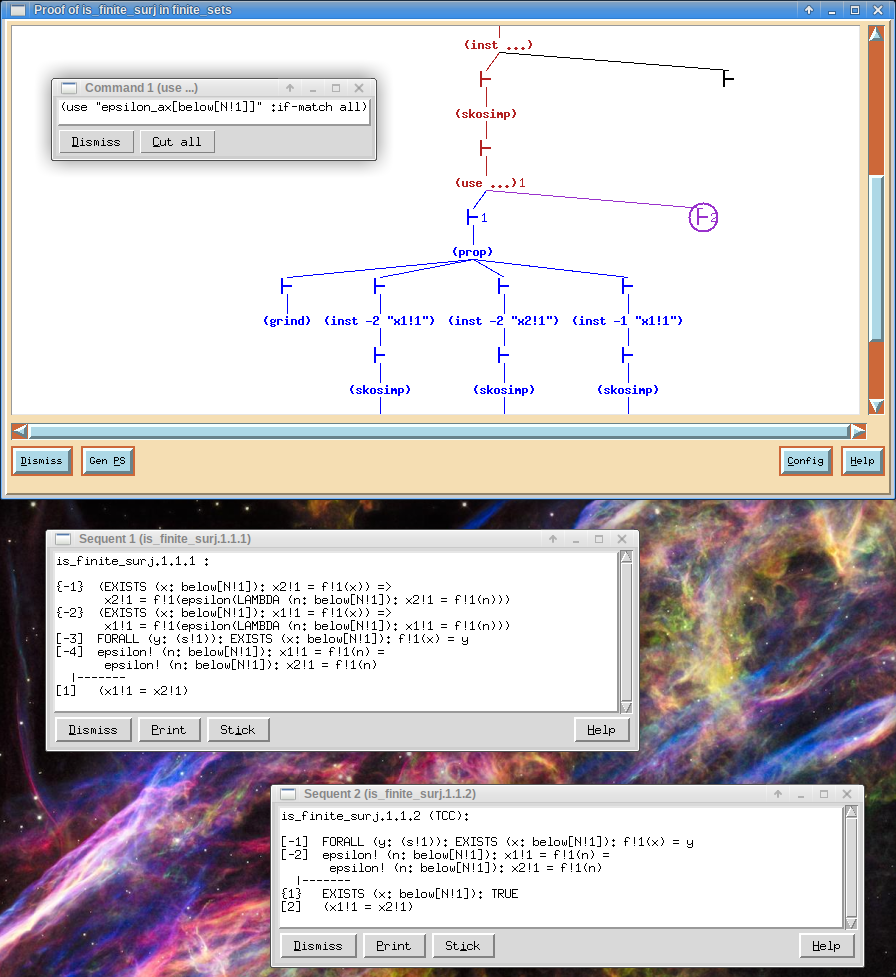
\includegraphics[width=\textwidth]{proofwindows.png}  
\caption{A Proof Display Example}\label{proofwindow}
\end{figure}

Colors are used to display status information about the proof.  These
colors may be specified using the X resource database (i.e., in your
\texttt{.Xresources} or \texttt{.Xdefaults} file).  Stipple patterns may
be specified instead of colors; a stipple pattern is specified as
\texttt{@file}, where \texttt{file} is either an absolute pathname of a
file in X bitmap format or the special bitmap name
\texttt{gray}.\footnote{If \texttt{file} is not an absolute path, it is
looked up in the \texttt{wish} subdirectory of the PVS directory, which
contains the \texttt{gray} bitmap.}

The current resources and their defaults are:

\begin{center}
\begin{tabular}{|lll|}\hline
  {\it Resource name} & {\it Color default} & {\it Monochrome default}%
     \\ \hline
  \texttt{pvs.windowbackground} & wheat & white \\
  \texttt{pvs.displaybackground} & white & white \\
  \texttt{pvs.displayforeground} & black & black \\
  \texttt{pvs.activedisplaybackground} & mediumslateblue & black \\
  \texttt{pvs.activedisplayforeground} & white & white \\
  \texttt{pvs.buttonbackground} & lightblue & white \\
  \texttt{pvs.buttonforeground} & black & black \\
  \texttt{pvs.activebuttonbackground} & steelblue & black \\
  \texttt{pvs.activebuttonforeground} & white & white \\
  \texttt{pvs.troughcolor} & sienna3 & black \\
  \texttt{pvs.currentColor} & DarkOrchid & black \\
  \texttt{pvs.circleCurrent} & yes & yes \\
  \texttt{pvs.tccColor} & green4 & black \\
  \texttt{pvs.doneColor} & blue & @gray \\
  \texttt{pvs.ancestorColor} & firebrick & black \\
  \texttt{pvs.abbrevLen} & 35 & 35 \\
  \texttt{pvs.displayfont} & \multicolumn{2}{l|}{lucidasanstypewriter-bold-12} \\
  \texttt{pvs.buttonfont} & \multicolumn{2}{l|}{lucidasanstypewriter-10} \\
  \texttt{pvs.proof.geometry} & \multicolumn{2}{l|}{\hspace*{.5in}\emph{none}} \\
  \texttt{pvs.theory-hierarchy.geometry} & \multicolumn{2}{l|}{\hspace*{.5in}\emph{none}} \\
  \texttt{pvs.prover-commands.geometry} & \multicolumn{2}{l|}{\hspace*{.5in}\emph{none}} \\
  \hline
\end{tabular}
\end{center}

The \texttt{foreground} color is used for things that aren't otherwise
specified below.  The \texttt{currentColor} is used for the current
sequent in the proof tree.  The \texttt{ancestorColor} is used for all
the ancestors of the current sequent, up to the root.  The
\texttt{doneColor} is used for sequents which have been proved.  The
\texttt{tccColor} is used for TCC's.  When \texttt{pvs.circle\-Current}
is set, the current sequent in the proof tree is circled.

Proof commands which are longer than \texttt{abbrevLen} characters are
abbreviated.

If the Emacs variable
\texttt{pvs-x-show-proofs}\index{pvs-x-show-proofs@\texttt{pvs-x-show-proofs}}
is not \texttt{NIL}, then \cmd{prove} automatically calls
\cmd{x-show-proof}.  This can be set in your
\texttt{.pvsemacs}\index{.pvsemacs@\texttt{.pvsemacs}} file.

The \cmd{x-theory-hierarchy} command prompts for a theory name and
displays the \texttt{IM\-PORTING} hierarchy rooted at that theory.  In a
complex hierarchy, it can be difficult to follow the lines; to make
this easier, when you move the mouse onto a theory identifier, all the
lines connecting that theory to other theories turn the
\texttt{highlight} color.  Clicking on a theory identifier will bring
up the theory in Emacs.  Figure~\ref{x-hierarchy} shows an example of the
theory hierarchy for the \texttt{finite\_sets} library, as produced from
clicking on the \texttt{Gen PS} button and selecting \texttt{portrait}.

\begin{figure}
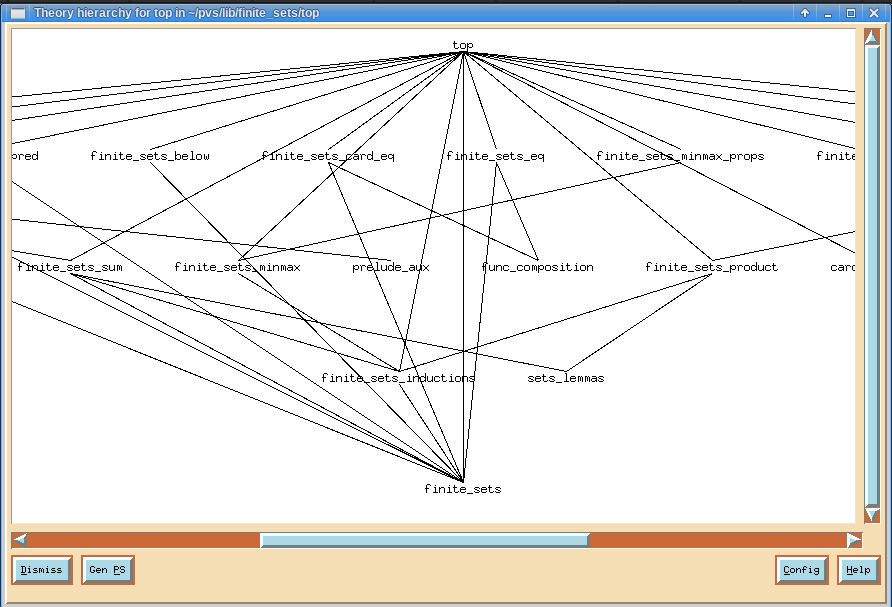
\includegraphics[width=\textwidth]{finite_sets_top_hier.png}
\caption{The Theory Hierarchy for the \texttt{finite\_sets} Library}\label{x-hierarchy}
\end{figure}


The remainder of this section applies to both \cmd{x-show-proof} and
\cmd{x-theory-hierarchy}.

The layout in the windows created by these commands can be manually
edited.  The editing commands are accessed by holding down the
\texttt{Control} key while pressing mouse buttons. In a proof window,
pressing \texttt{Control}-button~1 and dragging moves a whole proof
subtree, while \texttt{Control}-button~2 moves a single sequent.  In a
theory hierarchy window, \texttt{Control}-button~1 moves a theory.
(Note that most proof commands will do a relayout.)  Once the layout
is to your liking, the \texttt{Gen~PS} button will generate a
PostScript file which contains the contents of the window.  The
filename will be briefly displayed below the buttons.

The \texttt{Config} button will bring up a menu which will let you
customize the horizontal and vertical separations used by the
automatic layout for the current window.  These can also be customized
with the resource database.

\begin{center}
\begin{tabular}{|ll|}\hline
  {\it Resource name} & {\it Default} \\ \hline
  \texttt{pvs*proof*xSep} & 10 \\
  \texttt{pvs*proof*ySep} & 20 \\
  \texttt{pvs*th-hier*xSep} & 50 \\
  \texttt{pvs*th-hier*ySep} & 100 \\
  \hline
\end{tabular}
\end{center}


\section{Context Commands}

\begin{pvscmds}
\icmd{list-pvs-files} & \icmd{lf} & Display a list of PVS files in current context \\
\icmd{list-theories} & \icmd{lt} & Display a list of theories in current context \\
\icmd{change-context} & \icmd{cc} & Switch to a new context \\
\icmd{save-context} & \icmd{sc} & Save the current context \\
\icmd{pvs-remove-bin-files} & & Remove the \texttt{.bin} files of the current
context \\
\icmd{pvs-dont-write-bin-files} & & Inhibit writing or loading of
\texttt{.bin} files \\ 
\icmd{pvs-do-write-bin-files} & & Allows writing and loading of
\texttt{.bin} files (default) \\
\icmd{context-path} & \icmd{cp} & Display pathname of current context \\
\end{pvscmds}

The \cmd{list-pvs-files} and \cmd{list-theories} commands prompt for a
directory, default is to the current directory; if there is a PVS
context in the given directory, these commands list the PVS files or
theories in that context.  The resulting buffer is in a special mode,
which allows the file/theory to be viewed (by typing a ``\texttt{v}''),
selected (by typing a ``\texttt{s}'') or imported (by typing an ``{\tt
i}'').  A file or theory may only be selected if it is in the current
context, and may only be imported if it is not.  Importing a theory from
the list of theories will import the associated file.

The \cmd{change-context} command is similar to the ``\texttt{cd}'' command
in \unix; it saves the context (see below), and changes the working
directory to the specified one.  The \ibuf{PVS Welcome} buffer is then
displayed indicating the new directory.  If the requested directory does
not exist, and the Emacs you are running supports \texttt{make-directory},
then PVS offers to make a new one, including parent directories if necessary.
If the command fails for any reason, then the current context
stays the same.

The \cmd{save-context} command saves the current state of the session in
the context file \texttt{.pvscontext}.  In addition, any PVS files that
have been typechecked will generate a binary (\texttt{.bin}) file, unless
there is already a current one saved, or the \cmd{dont-write-bin-files}
command has been invoked.

Under normal circumstances, binary (\texttt{.bin}) files \index{.bin@\texttt{.bin}} corresponding to
the specification (\texttt{.pvs}) files are updated or created as needed.
These binary files contain type information, so that loading a binary file
has the same effect as typechecking the corresponding PVS file, but is
generally much faster.  The down side is that binary files take more disk
space.  If that is a problem then use the \cmd{pvs-dont-write-bin-files},
which neither loads nor creates binary files.  This can be added to your
\texttt{.pvsemacs}\index{.pvsemacs@\texttt{.pvsemacs}} file, by adding the
line
\begin{alltt}
  (pvs-dont-write-bin-files)
\end{alltt}
The \cmd{pvs-do-write-bin-files} undoes the effect of the
\cmd{pvs-dont-write-pvs-files}, and is not needed normally.  The
\cmd{pvs-remove-bin-files} command may be used to remove the binary files
that have been created.

The \cmd{context-path} command uses the minibuffer to display the
directory path associated with the current context.

\glossary{[directory path:] a file pathname containing sufficient
components to uniquely identify a directory}
\glossary{[context path:] a file pathname identifying the
directory which contains the context}

\section{Library Commands}

\begin{pvscmds}
\icmd{load-prelude-library} & & Extend the prelude from the specified context \\
\icmd{remove-prelude-library} & & Remove the specified context from the
prelude \\
\end{pvscmds}

The \cmd{load-prelude-library} command prompts for a context pathname
(\ie directory), and extends the prelude with all of the theories that
make up that context.  Note that the theories that make up the context are
defined by the \texttt{.pvscontext} file in the associated
directory---there may be specification files in the same directory that
are not a part of the context.  The files that make up the context are
typechecked if necessary, and internally the prelude is extended.  All of
the theories of the current context are untypechecked, as they may not
typecheck the same way in the extended prelude.  The PVS context is
updated to reflect that the prelude has been extended.  Thus the next time
this context is entered, the prelude will automatically be extended (by
typechecking the libraries if necessary).

This is just one of two means of gaining access to theories of a different
context (short of copying them).  For an alternative approach see the
language guide~\cite{PVS:language}.

The \cmd{remove-prelude-library} command removes the specified library
from the prelude.  It reverts all the theories of the current context to
untypechecked to guarantee that no theories depend on the removed library.
Note that the built-in prelude may not be removed this way.

\section{Browsing}

\begin{pvscmds}
\icmd{show-declaration} & \key{M-.} & Show declaration of symbol at cursor
\\
\icmd{goto-declaration} & \key{M-'} & Go to declaration of symbol at cursor \\
\icmd{find-declaration} & \key{M-,} & Search for declarations of given symbol \\
\icmd{whereis-declaration-used} & \key{M-;} & Search for declarations which reference identifier \\
\icmd{whereis-identifier-used} & \key{C-M-;} & Search for declarations which reference identifier \\
\icmd{list-declarations} & \key{M-:} & Produce list of declarations in import chain \\
\icmd{show-expanded-form} & \key{C-.} & Show expanded form of term
containing region\\
& & \emph{Arg:} also expand names from the prelude \\
\end{pvscmds}

These commands browse a specification consisting of several PVS files
and theories, providing information about where entities are declared
and used.  All of these commands browse the prelude as well as user
files.

The \cmd{show-declaration} command is used to determine the declaration
associated with the symbol or name at the cursor.  Positioning the cursor
on a name in the specification and typing \key{M-.} yields a pop-up
buffer displaying the declaration.  This command is useful to determine
the type of a name, or the resolution determined by the typechecker for an
overloaded name.  Note that when used on a record accessor it will
display the declaration of the record rather than just the record field.

The \cmd{goto-declaration} command goes to the declaration associated with
the symbol or name at the cursor.  It pops up a buffer containing the
theory associated with the declaration, and positions the cursor at the
declaration.

The \cmd{find-declaration} command takes a name and returns a list of all
the declarations with that name, the default name is the one under the
cursor. Each row in the display specifies the declaration name, its
kind/type, and the theory to which it belongs.  Declarations in this list
may be viewed by placing the cursor on the row of interest and typing
``\texttt{v}.''  Typing ``\texttt{s}'' will read in the associated file
and position the cursor at the declaration.  A ``\texttt{q}'' quits and
removes the declaration buffer.

The \cmd{whereis-declaration-used} command generates a list of
declarations which reference the entity denoted by a given identifier.
The related \cmd{whereis\-identifier-used} command generates a list of all
references to a \emph{textually identical} identifier, which may or may
not result from the same declaration, due to overloading and multiple
declarations.  The \cmd{list-declarations} command generates a listing of
all the declarations in the import chain of the specified theory.  For all
of these commands, the resulting buffer behaves exactly as described for
\icmd{find-declaration}.

The \cmd{show-expanded-form} command displays the expanded form of the
term containing the region in the \texttt{Expanded Form} buffer.  Each
variable, constant and operator is expanded to its full name including the
theory name and its parameters, unless they are from the current theory or
the prelude.  With an argument, prelude names are also expanded.  If the
region is not defined, the current cursor location is used instead.

%\memo{How about a \LaTeX\ version?}

\section{Theory Status}

\begin{pvscmds}
\icmd{status-theory} & \icmd{stt}, \key{C-c C-s t} & Status of specified theory (parsed, etc.) \\
\icmd{status-pvs-file} & \icmd{stf}, \key{C-c C-s f} & Status of theories of current file \\
\icmd{status-importchain} & \icmd{sti}, \key{C-c C-s i}  & Status of theories in import chain of theory \\
\icmd{status-importbychain} & \icmd{stb}, \key{C-c C-s b} & Status of
theories in import by chain \\
\end{pvscmds}

These commands provide information regarding the status of the
specified theories.  The status information for a theory indicates whether
it is parsed or typechecked, and provides the number of formulas, the
number proved, the number of TCCs generated, and the number of TCCs
proved.  Note that the number of formulas does not include the TCCs.

The number of theory warnings and messages is also displayed.  See the
\cmd{show-theory-warnings} and \cmd{show-theory-messages} on
page~\pageref{tc-info} for more information on these commands.

The \cmd{status-theory} command provides the status of the specified
theory in the mini\-buffer.  The \cmd{status-pvs-file},
\cmd{status-importchain}, and \cmd{status\-importbychain} commands display
the information in the \ibuf{PVS Status} buffer with a line for each
theory.  Using any of these commands on the \texttt{sum} theory yields
{\small
\begin{alltt}
sum is typechecked: 1 formula, 1 proved; 2 TCCs, 2 proved; 0 warnings; 0 msgs
\end{alltt}}
The \cmd{show-theory-warnings} and \cmd{show-theory-messages}
(page~\pageref{tc-info}) may be used to see any warnings or messages.

The \cmd{status-importchain} and \cmd{status-importbychain} commands
display the \texttt{IM\-PORT\-ING} chains of the specified theory, indented to
indicate the tree structure.  The \cmd{status-importchain} command works
recursively down the \texttt{IMPORTING}s, displaying the status of each
theory unless it has been displayed earlier in the buffer.  The
\cmd{status-importbychain} works in the opposite direction.


\section{Proof Status}
\label{proof-status}

\begin{pvscmds}
\icmd{status-proof} & \icmd{sp}, \key{C-c C-s p} & Status of formula at cursor \\
\icmd{status-proof-theory} & \icmd{spt} & Status of formulas in theory \\
 & & \emph{Arg:} provide timing information \\
\icmd{status-proof-pvs-file} & \icmd{spf} & Status of formulas in PVS file \\
 & & \emph{Arg:} provide timing information \\
\icmd{status-proof-importchain} & \icmd{spi} & Status of formulas on importchain \\
 & & \emph{Arg:} provide timing information \\
\icmd{status-proofchain} & \icmd{spc} & Proofchain of formula at cursor \\
\icmd{status-proofchain-theory} & \icmd{spct} & Proofchain of
specified theory \\
\icmd{status-proofchain-pvs-file} & \icmd{spcf} & Proofchain of current file \\
\icmd{status-proofchain-importchain} & \icmd{spci} & Proofchain of importchain \\
\end{pvscmds}

These commands provide the status of the proofs of the indicated formulas.
The \cmd{status-proof} command uses the minibuffer to display the proof
status of the formula at the cursor.  The status can be one of
\texttt{proved}, \texttt{untried}, \texttt{unfinished}, or
\texttt{unchecked}.  Untried means that the proof has not yet been
attempted.  Unfinished means that the proof has been attempted,
but is not complete.  Unchecked means that the proof was successful at one
point, but that some changes have been made that may invalidate the proof.

The commands \cmd{status-proof-theory}, \cmd{status-proof-pvs-file}, and
\cmd{status\-proof-importchain} use the \ibuf{PVS Status} buffer
to display the proof status for all of the formulas within the theory, PVS
file, or the import chain respectively.  With an argument, these commands
display timing information as well.

The \cmd{status-proofchain} command provides a proof chain analysis of the
formula at the cursor and displays it in the \ibuf{PVS Status} buffer.
The proof chain analysis indicates whether the formula has been proved,
and analyses the formulas used in the proof to insure that the proof is
complete; lemmas used in the proof are proved and sound, \ie\ there are no
circularities (for example, using lemma $\mathcal{A}$ to prove
$\mathcal{B}$ and vice-versa).  Because judgements are used implicitly,
they may be included in the analysis even if they are not actually used.

The commands \cmd{status-proofchain-theory},
\icmd{status-proofchain-pvs-file}, and \newline
\icmd{status-proofchain-importchain} provide the proof chain analysis for
each formula of the theory, PVS file, and import chain of the specified
theory, respectively, in the \ibuf{PVS Status} buffer.

\section{Environment Commands}

\begin{pvscmds}
\icmd{whereis-pvs} & & Display the root PVS directory \\
\icmd{pvs-version} & & Display current version of PVS and underlying \lisp \\
\icmd{pvs-mode} & & Put current buffer in PVS mode \\
\icmd{pvs-log} & & Display the \ibuf{PVS Log} buffer \\
\icmd{status-display} & & Display the \ibuf{PVS Status} buffer \\
\icmd{pvs-status} & & Find out if PVS is busy \\
\icmd{pvs} & & Start the PVS process \\
\icmd{pvs-load-patches} & & Load new PVS patches \\
\end{pvscmds}

The \cmd{whereis-pvs} command is used to determine the directory where the
PVS system resides.  This is useful for finding the example specifications
and files that are part of the PVS distribution.

The \cmd{pvs-version} command displays the current version of PVS\@.

The \cmd{pvs-mode} command puts the current buffer in PVS mode.  This
command is not normally needed; buffers with a \ibuf{.pvs}
extension and buffers created by PVS are automatically put in the
proper mode.

Most of the messages that appear in the minibuffer are kept in the
\ibuf{PVS Log} buffer, stamped with the time.  The \cmd{pvs-log} command
simply pops up the \ibuf{PVS Log} buffer so that you may view it.

The \cmd{status-display} command simply displays the \ibuf{PVS Status}
buffer.  This is the buffer used for most of the status commands.

The \cmd{pvs} command is what is used to actually start PVS after the
Emacs files have all been loaded.  It is provided as a user command
because there are times when the PVS lisp subprocess has been killed and
you wish to start up that process while keeping the same Emacs session.

The \cmd{pvs-load-patches} command reloads the patches.  This is useful
when new patches have been installed, and you wish to load them without
exiting the system and starting up again.


\section{Interrupting PVS}

\begin{pvscmds}
\icmd{pvs-status} & & Find out if Lisp is busy \\
\icmd{pvs-interrupt-subjob} & \key{C-c C-c} & Interrupt PVS (lisp)
  process \\
\icmd{reset-pvs} & \key{C-z C-g} & Abort PVS and resynchronize \\
\end{pvscmds}

Many PVS commands run in the background, allowing other editing
activities to proceed concurrently.  The effect of issuing new commands
while another command is running depends on the command: 
background commands placed on the command queue.  Other (nonbackground
commands) interrupt the currently running command, execute, and return
control to the interrupted command.  The Emacs status line indicates
the abbreviation of the command that is currently running, if any, or {\tt
ready}.  The \cmd{pvs-status} command provides information
about both the currently running command and the command queue.

To interrupt PVS for any reason, the following procedure is recommended.
First, if the keyboard is not responding, type the built-in Emacs
command \cmd{keyboard-quit} (\key{C-g}); it may need to be struck a few
times before there is any response---usually a beep and \texttt{Quit}
appears in the minibuffer.  This command interrupts Emacs, but has no
effect on any PVS commands that are still running.  After Emacs responds
go to the end of the \texttt{*pvs*} buffer, and type \key{C-c C-c}.  If
Lisp is able to respond, you should see the message
{\small\small
\begin{alltt}
Error: Received signal number 2 (Keyboard interrupt)
  [condition type: INTERRUPT-SIGNAL]

Restart actions (select using :continue):
 0: continue computation
 1: Return to Top Level (an "abort" restart)
[1c] PVS(22):
\end{alltt}}
You can then type \texttt{:continue 0} to keep going as it was never
interrupted, \texttt{(restore)} if you are in the middle of an ongoing
proof and want to continue from the state prior to the last \emph{atomic}
prover command (see the prover guide~\cite{PVS:prover}), or
\texttt{:continue 1} or \texttt{:reset} to abort to the top level.

The Lisp process may not be able to respond to the interrupt right away,
especially if it has started garbage collection.  If you really want to
interrupt it, type more \key{C-c C-c} interrupts; after about six of them
it is supposed to respond regardless.  This is not recommended in general
as it can leave the Lisp process in an unstable state.  Unfortunately, we
have seen Allegro Common Lisp get into a state where it is completely
unresponsive, even after several interrupts and waiting for hours for a
response.  This is rare, but if it happens the only recourse is to kill
the process and start up a new PVS session.  See below for how to do this
while allowing Emacs to continue.

The \cmd{reset-pvs} command aborts any ongoing activity in PVS; its
effects depend on whether it is issued from the \ibuf{*pvs*} buffer or
from some other buffer.  In the former case, \cmd{reset-pvs} simply
interrupts PVS as if you typed \key{C-c C-c}, as described above.  If
\cmd{reset-pvs} is issued somewhere other than the \ibuf{*pvs*} buffer,
you are asked whether to reset PVS in case the command was typed
accidentally; if not, the current command is aborted and the command queue
is emptied.

If you wish to kill the PVS Lisp process, while keeping your current Emacs
session, simply go to the \texttt{*pvs*} buffer and kill it
\icmd{kill-buffer} \key{C-x k}, then run \icmd{pvs} and the PVS Lisp
process will restart.  All your other Emacs buffers are unaffected by
this.

\setcounter{footnote}{0}
% Document Type: LaTeX
% Master File: user-guide.tex
\chapter{Customizing PVS}
\label{customization}
\index{customization}\index{PVS customization}

PVS is a complex system, and utilizes many subsystems, including Lisp,
Emacs, the X window system, and Tcl/Tk.  You can control aspects of these
subsystems by a combination of command-line arguments, environment
variables, and various files.  In this section we discuss some aspects of
the customization of these subsystems as they relate to PVS.

\section{Invoking PVS}\label{invoking-pvs}
\index{invoking PVS}\index{starting PVS}

PVS is invoked from a shell script named \texttt{pvs}\index{PVS shell
script} in the PVS directory---this is a text file, and may be examined or
copied and modified to suit your taste.  The script is a Bourne shell
script, and requires {\tt /bin/sh} to execute correctly.\footnote{On some
systems, \texttt{/bin/sh} is linked to the \texttt{bash} shell; this works
as well.}

PVS accepts a number of command-line arguments\index{PVS!command-line
arguments}\index{command-line arguments}, as well as using environment
variables.  The command-line arguments specific to PVS are
\begin{description}

\item[\texttt{-h | -help | --help}]\index{-help@\texttt{-help} command
line argument} - Print a brief description of the command line options and
exit.

\item[\texttt{-lisp} \emph{lispname}]\index{-lisp@\texttt{-lisp} command
line argument} - Specifies which lisp to use. The lisp image used for PVS
is then \texttt{pvs-\emph{lispname}}, which should be located in a
directory determined by the machine architecture.  See
Section~\ref{pvsimage}, page~\pageref{pvsimage} for details.

\label{dash-redhat}
\item[\texttt{-redhat}
\emph{redhat-release}]\index{-redhat@\texttt{-redhat} command line
argument} - Specifies the release of the Redhat Linux operating system you
are using (different PVS binaries are required for libc5 and glibc C
libraries).  PVS attempts to discover this for itself, but if the wrong
binary is chosen you can specify \texttt{4} or \texttt{5} using this
argument.  Note that Redhat 6 uses the glibc libraries, which corresponds
to the value \texttt{5}.

\item[\texttt{-runtime}]\index{-runtime@\texttt{-runtime} command line
argument} - This is only needed at SRI, where the development version of
the system is used by default.  With this option the runtime image is used
instead.

\item[\texttt{-emacs} \emph{emacsname}]\index{-emacs@\texttt{-emacs}
command line argument} - Specifies the Emacs to use; see below for
details.

\item[\texttt{-decision-procedures}
\emph{new}\texttt{|}\emph{old}]\index{-decision-procedures@\texttt{-decision-procedures}
command line argument} - Sets the default decision procedures to be used
in proofs.  See Section~\ref{decision-procedure-commands},
page~\pageref{decision-procedure-commands} for details.

\item[\texttt{-force-decision-procedures}
\emph{new}\texttt{|}\emph{old}]\index{-force-decision-procedures@\texttt{-force-decision-procedures}
command line argument} - Forces the chosen decision procedure to be used
regardless of the default decision procedure setting or which decision
procedures were used in developing a proof.  Note that with this option
there is no way to switch between the new and old decision procedures.

\item[\texttt{-nw}]\index{-nw@\texttt{-nw} command line argument} - Tells
Emacs not to use its special interface to X.

\item[\texttt{-batch}]\index{-batch@\texttt{-batch} command line argument}
- Run PVS in batch mode. See chapter~\ref{batchmode},
page~\pageref{batchmode} for details.

\item[\texttt{-timeout}:]\index{-timeout@\texttt{-timeout} command line
argument} In batch mode, this causes typechecking and individual proof
attempts to be interrupted after the given number of seconds.

\item[\texttt{-nobg}:]\index{-nobg@\texttt{-nobg} command line argument}
Normally PVS starts in the background (with the \& control operator).
This starts it in the foreground.

\item[\texttt{-raw}:]\index{-raw@\texttt{-raw} command line argument} This
runs PVS without Emacs.  This is only useful for front ends, which must do
the same initialization as done by the Emacs interface.

\item[\texttt{-v} \emph{number}]\index{-v@\texttt{-v} command line
argument} - Specifies verbosity level for PVS batch mode. See
Chapter~\ref{batchmode}, page~\pageref{batchmode} for details.

\label{dash-q-option}
\item[\texttt{-q}]\index{-q@\texttt{-q} command line argument} - A
standard emacs option to inhibit loading of the users {\tt .emacs} file,
but extended in PVS to inhibit loading of the users {\tt .pvsemacs}, {\tt
.pvsxemacs-options} and \texttt{.pvs.lisp} files on startup.

\item[\texttt{-patchlevel}
\emph{level}]\index{-patchlevel@\texttt{-patchlevel} command line
argument} - Specifies which patch files to load. Level \texttt{none} loads
no patch files. Level \texttt{rel} loads the file \texttt{patch2} from
your PVS directory, which usually contains the release versions of PVS
patches. Other valid levels are \texttt{test} (loads the files
\texttt{patch2} and \texttt{patch2-test}) and \texttt{exp} (loads the
files \texttt{patch2}, \texttt{patch2-test} and \texttt{patch2-exp}).
This option is mainly used for PVS development.


\end{description}
Any other command-line arguments are passed directly to the underlying
Emacs, including those for X windows---these are discussed
below.

In addition, the PVS script uses the environment
variables\index{PVS!environment variables}\index{environment variables}
\texttt{PVSLISP}\index{pvslisp@\texttt{PVSLISP}}\index{environment
variables!pvslisp@\texttt{PVSLISP}},
\texttt{PVSEMACS}\index{pvsemacs@\texttt{PVSEMACS}}\index{environment
variables!pvsemacs@\texttt{PVSEMACS}}, and
\texttt{PVSXINIT}\index{pvsxinit@\texttt{PVSXINIT}}\index{environment
variables!pvsxinit@\texttt{PVSXINIT}}, which may be set in your
\texttt{.cshrc} or \texttt{.login} file to specify the defaults you
prefer.  If both the environment variable and the corresponding
command-line argument are given, the command-line argument takes
precedence.  The \texttt{PVSXINIT} variable is described in
Section~\ref{windows}, page~\pageref{windows}.


\section{Emacs}
\index{Emacs|(}

The PVS system uses Emacs as its user interface, and provides a number of
files that extend Emacs for use with PVS.  For historical reasons, there
are currently a number of Emacs editors available.  Because we wanted PVS
to be freely available, we have chosen to concentrate on just \gnuemacs\
and XEmacs, which are also freely available.  To find out what version of
Emacs you are using, start up Emacs and type \iecmd{emacs-version}.  We
try to keep up with new releases of emacs and if necessary patch files
will be made available to support the new Emacs.

By default, the system uses \texttt{emacs}, which is assumed to be in your
path when you start up PVS.  You may specify a different Emacs as
specified above.  When you start PVS, is assumed (in order to supply X
resources in the correct format) that if the name of the emacs command
contains the character ``\texttt{x}'' then you are using XEmacs.

PVS loads your \texttt{\char'176/.emacs}\index{.emacs@\texttt{.emacs}}
file first (assuming you have not specified the {\tt -q} option as
described on page \pageref{dash-q-option}), followed by
\emph{PVSPATH}\texttt{/emacs/go-pvs.el}%
\index{go-pvs.el@\texttt{go-pvs.el}}, which determines which version of
emacs you are running and then loads the rest of the PVS emacs files,
including ILISP\index{ILISP}.  At this point you may receive an error from
PVS saying that your Emacs version is unknown.  PVS does not support Emacs
18 (or earlier), but we try to keep up with new Emacs versions as they are released.
Finally, the
\texttt{\char'176/.pvsemacs}\index{.pvsemacs@\texttt{.pvsemacs}} is
loaded.  If you are running XEmacs, the {\tt .pvsemacs} file will load
XEmacs options from the {\tt .pvsxemacs-options} file instead of the
standard {\tt .xemacs-options} file, as some are incompatible with
standard XEmacs.

In loading the files in this order, PVS functions and key
bindings will overwrite any conflicting ones defined in your
\texttt{.emacs} file.  \texttt{.pvsemacs} is the file to use to override
the key bindings and definitions given by PVS.  This approach was taken to
ensure that the behavior of PVS by default follows the user guide, but can
be readily modified to suit your taste.

One file that is worth noting is the
\emph{PVSPATH}\url{/emacs/emacs-src/pvs-abbreviations.el}%
\index{pvs-abbreviations.el@\texttt{pvs-abbreviations.el}} file, where the
abbreviations for many of the PVS commands are given.  You may define your
own abbreviations for commands you use a lot that don't currently have
abbreviations, by adding the appropriate lines in your \texttt{.pvsemacs}
file.  For example, adding
\begin{alltt}
  (pvs-abbreviate 'show-tccs 'st)
\end{alltt}
will make \ecmd{st} an abbreviation for \ecmd{show-tccs} in addition to
those already defined.  Note that you cannot redefine a name which is
already in use.

If you would like to byte-compile your Emacs customizations, create a
separate file, byte-compile it, and load it from your \texttt{.pvsemacs}.
Generally the kinds of forms provided in a \texttt{.pvsemacs} file are
simply variable settings and minor function definitions, and are not worth
byte-compiling.  It is only worthwhile if a function is being (re)defined
that will be invoked noninteractively and frequently, for example, if you
want to modify the way the process filter works.

\index{Emacs|)}


\section{The PVS Image}
\label{pvsimage}\index{PVS!lisp image|(}

PVS currently runs under Allegro Common Lisp on a number of different
platforms.  PVS is provided as a Common Lisp image, meaning that it
includes both the Lisp runtime system and the PVS programs, so you do not
need to have Allegro installed on your system.

There is usually just one PVS image available at a given site, and if the
system is properly installed, nothing further needs to be done.  If more
than one image is available, and the default one is not the desired one,
then it can be specified using either command-line arguments or
environment variables.  Invoking PVS with
{\smaller
\begin{alltt}
  pvs -lisp lucid -image pvs-lucid-sun4
\end{alltt}}
\noindent will use the \texttt{pvs-lucid-sun4} image.  Note that \texttt{-lisp
lucid} must be specified, so that the Emacs interface can be set up
properly.  For linux, also see the {\tt -redhat} option on page
\pageref{dash-redhat}.

Alternatively, the environment variables \texttt{PVSLISP} and
\texttt{PVSIMAGE} may be set to get the same effect.  Note that
command-line arguments take precedence.

After the PVS lisp image has started, it loads in the patch files as
specified by the {\tt -patchlevel} argument and then loads the file
{\tt .pvs.lisp} from your home directory.  This file can be used to
provide lisp customizations on a per user basis and for overriding
definitions in the patch file.

\index{PVS!lisp image|)}


\section{Window Systems}
\label{windows}

PVS was built primarily for the X window system\index{X windows}, though
it can be run from a terminal interface.
When run under X windows with the 
supported versions of Emacs, the resource name\index{resource
name}\index{PVS!resource name} will be set to \texttt{PVS}, and the
window\index{window name}\index{PVS!window name} and icon names\index{icon
name}\index{PVS!icon name} will be set to \texttt{PVS@}\textit{host\/},
where \textit{host\/} is the host name of the system on which PVS was
invoked.  These may be modified by adding command-line arguments or
setting the \texttt{PVSXINIT}\index{pvsxinit@\texttt{PVSXINIT}}%
\index{environment variables!pvsxinit@\texttt{PVSXINIT}} environment
variable.

You may customize the title and icon names by defining the function
\texttt{pvs-title-string} in your \texttt{.pvsemacs} file taking no
arguments and returning a string to be used as the title.  This function
is invoked at startup, and whenever the context is changed.  For example,
the following provides the name of the pvs path, the patch level
(\texttt{N} for none, \texttt{R} for released, \texttt{T} for test, and
\texttt{E} for experimental), the hostname, and the last two components of
the current context.

{\smaller
\begin{alltt}
    (defun pvs-title-string ()
      (format "%s%s%s:%s/"
          (trailing-components pvs-path 1)
        (cond ((stringp (cadddr *pvs-version-information*)) "E")
              ((stringp (caddr *pvs-version-information*)) "T")
              ((stringp (cadr *pvs-version-information*)) "R")
              (t "N"))
        (let ((host (car (string-split ?. (getenv "HOSTNAME")))))
          (format "@%s" host))
        (trailing-components *pvs-current-directory* 2)))
\end{alltt}}
\noindent For example, this might generate \url{pvs2.3N@photon:lib/finite_sets/}.

It is difficult to get a single setting for all of the Emacs versions; the
following table gives the arguments needed to set the resource, window,
and icon names for the various versions.

\begin{center}
\begin{tabular}{|l|l|l|l|} \hline
Emacs & Resource & Window & Icon \\ \hline\hline
emacs19 & \texttt{-rn} & \multicolumn{2}{|c|}{\texttt{-name}}\\ \hline
emacs19.29 (and later, & \multicolumn{3}{|c|}{\texttt{-name}}\\ 
including emacs20) & \multicolumn{3}{|c|}{ }\\ \hline
xemacs & \texttt{-name} & \texttt{-wn} & \texttt{-in} \\ \hline
\end{tabular}
\end{center}
\par\noindent Note: in emacs19, if \texttt{-rn} is not given, then
\texttt{-name} is used for the resource name as well.  Emacs19.29 and
later will give an error if the \texttt{-rn} argument is given.

The window name is the name used in the title bar of the PVS window, the
icon name is the name used in the icon, and the resource name is the name
referred to in the \texttt{.Xdefault} or \texttt{.Xresource} file that
controls the defaults for X clients.  An example entry for PVS in one of
these files might be
\begin{alltt}
!	PVS defaults
PVS.geometry: 80x63-0-0
PVS*pointerColor: Red
PVS*Font: *courier-medium-r-normal--12*
\end{alltt}
See the man pages for \texttt{X} and \texttt{emacs}, as well as the news
and info pages for the version of Emacs you are using for more details on
X resources.

The \texttt{PVSXINIT} environment variable may be set\footnote{Generally
environment variables are set in your shell startup file, \emph{e.g.},
\texttt{.profile} or \texttt{.cshrc}.} to a string
of command-line arguments that are then appended to the defaults described
above.  You can also change the default resource, window, and icon names,
simply by adding them to this variable (or by including them in the
command-line arguments).  Note that you should make certain that the
version of Emacs you are using matches the command-line arguments as shown
in the footnote.  You can tell that there is a mismatch when you start up
PVS and find buffers with names matching command-line arguments, \eg\
\texttt{-in} or \texttt{PVS@acorn}.

\setcounter{footnote}{0}
% Document Type: LaTeX
% Master File: user-guide.tex
% Use latex2e to process this file
\chapter{Running PVS in Batch Mode}
\label{batchmode}

To support validation runs, PVS supports a \emph{batch mode}, which
means that specifications and proofs being processed are not displayed.
In batch mode there is no direct interaction with PVS; it simply processes
whatever files or functions are provided and terminates after completing
the last of them.  PVS batch mode is built directly on the underlying
Emacs batch mode described in Section A.2 of the GNU Emacs
Manual~\cite{emacs20}.

If PVS is invoked in batch mode from a shell, then it may be interrupted
(using \texttt{C-c}), suspended (\texttt{C-z}), or run as a background
job.  The output may be redirected to a file or piped to another
command.\footnote{The Emacs batch option actually sends its output to
\texttt{stderr} rather than \texttt{stdout}; the \texttt{pvs} shell script
redirects this to \texttt{stdout}, as this is generally more useful and
easier to work with.}

To run PVS in batch mode, simply include the `\texttt{-batch}' option in
your call to PVS.  In addition, you should include one or more Emacs
source files and/or a Emacs or PVS function to run, using the `\texttt{-l}' or
`\texttt{-load}' option to load a file, and the `\texttt{-f}' or
`\texttt{-funcall}' option for a function.  For example:
\begin{alltt}
  pvs -batch -l test.el
  pvs -batch -f pvs-version
\end{alltt}
Note that the function option is severely limited, as it only allows a
function name.  This means that only functions that take no arguments may
be provided, for example, \texttt{pvs-version} or \texttt{whereis-pvs}.

Running PVS in batch mode does cause your \texttt{\char'176/.emacs} file
to be loaded, in contrast to running Emacs in batch mode.  If you want
to suppress the loading of your \texttt{.emacs}, include the
`\texttt{-q}' option, for example:
\begin{alltt}
  pvs -batch -q -l test.el
\end{alltt}

In batch mode PVS suppresses messages by default, though you can print
your own messages.  You can also control the amount of printout using the
verbose option, `\texttt{-v}', and providing a level number ranging from
\texttt{0} to \texttt{3}.
The following table summarizes the levels.
\begin{center}
\begin{tabular}{|l|l|}\hline
\textbf{level} & \textbf{printout} \\ \hline
0 & User-defined \texttt{pvs-message}s only \\
1 & Messages normally sent to the echo area and PVS errors\\
2 & Status buffers \\
3 & Proof replays \\ \hline
\end{tabular}
\end{center}

The \texttt{pvs-message} function is much like the Emacs \texttt{message}
function, but the message will get printed no matter what the level number
is.  If you want to print out only when the level is \texttt{1} or higher,
use \texttt{message} instead.  Both take a control string and an arbitrary
number of arguments.  An example is shown in Figure~\ref{batch-file}.

The file provided to the load option (`\texttt{-l}' or `\texttt{-load}')
is an ordinary Emacs file, and usually has an \texttt{.el} extension.
Inside this file you can invoke any PVS commands you want, though many of
them only make sense interactively.  For example, the \texttt{prove}
command expects the cursor to be positioned at a given formula, which is
difficult (though not impossible) to do in batch mode.  The various Tcl/Tk
commands available will not run at all because there is no X display
associated with PVS running in batch mode.  The most useful commands to
run in batch mode are listed in Table~\ref{batch-commands}.  In that table, a
\textit{filename} is a PVS file name without the \texttt{.pvs} extension,
a \textit{theoryname} is the name of a theory in the current context, and
a \textit{directory} is a Unix pathname.  These must all be given as
strings (enclosed in double quotes).  The \textit{length} and
\textit{depth} arguments are integers, and do not need any special
treatment.  PVS Emacs commands are given in Emacs lisp syntax; for
example,
\begin{alltt}
  (parse "foo")
  (set-print-depth 3)
  (save-context)
\end{alltt}

\begin{table}
\begin{center}
\begin{tabular}{|l|l|}\hline
\textbf{Command} & \textbf{Arguments} \\ \hline
\texttt{parse} & \textit{filename} \\
\texttt{typecheck} & \textit{filename} \\
\texttt{typecheck-importchain} & \textit{filename} \\
\texttt{typecheck-prove} & \textit{filename} \\
\texttt{typecheck-prove-importchain} & \textit{filename} \\
\texttt{prove-theory} & \textit{theoryname} \\
\texttt{prove-pvs-file} & \textit{filename} \\
\texttt{prove-importchain} & \textit{theoryname} \\
\texttt{set-print-depth} & \textit{depth} \\
\texttt{set-print-length} & \textit{length} \\
\texttt{set-rewrite-depth} & \textit{depth} \\
\texttt{set-rewrite-length} & \textit{length} \\
\texttt{alltt-theory} & \textit{theoryname} \\
\texttt{alltt-pvs-file} & \textit{filename} \\
\texttt{alltt-importchain} & \textit{theoryname} \\
\texttt{latex-theory} & \textit{theoryname} \\
\texttt{latex-pvs-file} & \textit{filename} \\
\texttt{latex-importchain} & \textit{theoryname} \\
\texttt{latex-set-linelength} & \textit{length} \\
\texttt{change-context} & \textit{directory} \\
\texttt{save-context} & \\
\texttt{pvs-remove-bin-files} & \\
\texttt{pvs-dont-write-bin-files} & \\
\texttt{pvs-do-write-bin-files} & \\
\texttt{status-theory} & \textit{theoryname} \\
\texttt{status-pvs-file} & \textit{filename} \\
\texttt{status-importchain} & \textit{theoryname} \\
\texttt{status-importbychain} & \textit{theoryname} \\
\texttt{status-proof-theory} & \textit{theoryname} \\
\texttt{status-proof-pvs-file} & \textit{filename} \\
\texttt{status-proof-importchain} & \textit{theoryname} \\
\texttt{status-proofchain-theory} & \textit{theoryname} \\
\texttt{status-proofchain-pvs-file} & \textit{filename} \\
\hline
\end{tabular}
\end{center}
\caption{Commands available for validation}\label{batch-commands}
\end{table}

An example of the contents of a batch file is shown in
Figure~\ref{batch-file}.  This file consists of three commands.  It prints
the message ``\texttt{Proving stamps2}'', changes to the
\texttt{\char'176/pvs/test} context, and then reruns all the proofs of the
specification file \texttt{stamps2.pvs}.  Note that
\texttt{current-prefix-arg} is set to \texttt{t} to ensure that the proofs
are retried.  This is equivalent to using \texttt{C-u} interactively.
\begin{figure}
\begin{center}
\fboxsep=10pt%
\begin{boxedminipage}{3.2in}
\begin{alltt}
(pvs-message "Proving stamps2")
(change-context "~/pvs/test")
(let ((current-prefix-arg t))
  (prove-pvs-file "stamps2"))
\end{alltt}
\end{boxedminipage}
\end{center}
\caption{Batch File Example}\label{batch-file}
\end{figure}
While PVS is running in batch mode, two possible kinds of error may be
encountered.  An Emacs error comes from badly formed batch files or
nonexistent functions.  These errors will cause the system to stop
immediately, and the error will be displayed if the level number is
nonzero.  A PVS error generates an error message (for a nonzero level
number) and abandons the current command, but allows the system to go on
to the next command.

If an emacs error is encountered that reports 'entering debugger' when
run with verbosity level 3, the full commands of the emacs debugger
are available\footnote{See the Emacs manual\cite{emacs20} for details.}.
A useful command to discover where your validation script encountered the error is:
\begin{alltt}
e (progn (set-buffer "*Backtrace*")(buffer-string))
\end{alltt}

Another potential pitfall is that PVS may appear to hang.  If this
happens, try running with verbosity level 3 as it is likely that PVS
is awaiting user input (usually a yes/no).  You may respond to such
prompts from the shell. 

\section{Validation Runs}

A validation run is simply a batch run in which the \texttt{pvs-validate}
macro is used in the batch file.  Given a \emph{log file} name, a
directory, and a sequence of PVS Emacs commands, \texttt{pvs-validate}
will change context to the specified directory and run the commands,
collecting the output into the log file.  It then compares the new results
to the previous ones, and reports whether there were any significant
differences.  An example of the use of \texttt{pvs-validate} is shown in
Figure~\ref{validate-file}.
\begin{figure}
\begin{center}
\fboxsep=10pt%
\begin{boxedminipage}{3.3in}
\begin{alltt}
(pvs-validate
  "stamps2.log"
  "~/pvs/test"
  (pvs-message "Proving stamps2")
  (set-rewrite-depth 0)
  (let ((current-prefix-arg t))
    (prove-pvs-file "stamps2")))
\end{alltt}
\end{boxedminipage}
\end{center}
\caption{Example Use of \texttt{pvs-validate}}\label{validate-file}
\end{figure}

Any number of \texttt{pvs-validate} forms may be used, and they may be
freely intermixed with other Emacs or PVS commands.  When the sequence of
commands associated with an invocation of \texttt{pvs-validate} is
complete, the log file is compared to the previous version, if it exists.
At this point PVS will report one of three messages:
\begin{itemize}
\item \texttt{Nothing to compare \textit{log} to} - the log file has not
been generated before this run.

\item \texttt{No significant changes in \textit{log}} - the current run
does not differ significantly from the last one.  A significant difference
is one that involves more than timing differences.  For example, the
message \texttt{proved in 27 seconds} is not significantly different from
\texttt{proved in 31 seconds}.

\item \texttt{Differences found since last run} - differences were
found.  The following line indicates the two log files that should be
compared to see where they differ.
\end{itemize}

This is normally all the output provided by PVS while processing a
\texttt{pvs-validate} macro, though you can get more information by
including the `\texttt{-v}' option as described above.

With minor exceptions, the log files contain the same information as
obtained with the `\texttt{-v 3}' option, but only for the commands of the
given \texttt{pvs-validate} macro.  In comparing log files, timings are
ignored.\footnote{In the future we may want to compare timings and report
those that are significantly different, but in order for this to work
properly we must get CPU times rather than real times, and make sure that
we are keeping track of the machine used for the previous validation run
For now we are only concerned with functional correctness.}

When a difference is reported, you can find out what the differences
actually are by starting up (an interactive) PVS, and bringing up the two
files in a split window.\footnote{In detail, start up PVS, use \texttt{C-x
C-f} to visit the first file, use \texttt{C-x 2} to split the window
vertically, and then use \texttt{C-x C-f} again to bring in the second
file.}  Then use \texttt{M-x pvs-compare-validation-windows}, which works
much like the Emacs \texttt{compare-windows} command, and will position
the cursor at the point where the two files differ.  Again, differences in
timing are ignored.  After analyzing the difference, you can move the
pointer in each buffer to the next position where they are the same, and
run \texttt{M-x pvs-compare-validation-windows} again to get to the next
difference.  In this way you can quickly analyze all the differences since
the last validation run.

The log files are maintained under RCS~\cite{RCS}, using the Emacs
\emph{Version Control} interface~\cite{emacs20}.  The first time
a validation run is made from a given directory, an RCS subdirectory is
created to keep the directory from being cluttered with RCS files.
If this is the first validation run for a given log file, then the log
file is created and registered to RCS.  In subsequent runs, the log file
is compared to the previous version, which will have a name including the
version number, for example, \texttt{stamps2.log.\char'176 1.8\char'176}.
If the comparison shows no significant differences, then the file is
subsequently deleted.

Note that the log files are all kept in the directory from which PVS was
run, and changing context will not affect that.  This makes it easy to
maintain a single directory that controls the validation for several
different contexts.

\section{Example Validation Run}
Here is an example of a validation run for a very simple specification.
\subsection{The Specification}
The specification is in the file \texttt{stamps.pvs}:
\begin{alltt}
stamps : THEORY
 BEGIN
  i, n3, n5: VAR nat
  stamps: LEMMA (FORALL i: (EXISTS n3, n5: i+8 = 3*n3 + 5*n5))
 END stamps
\end{alltt}
\subsection{The Validation File} 
The file \texttt{stamps.el} has the validation commands.  In this case we
are simply going to reprove the formulas of the specification file (there
is only one):
\begin{alltt}
(pvs-validate
 "stamps.log"
 "~/pvs-specs/validation"
 (pvs-message "Proving stamps")
 (let ((current-prefix-arg t))
   (prove-pvs-file "stamps")))
\end{alltt}
\subsection{The Validation Run}
Here is the validation run, with level number 1.  This shows the messages
that normally appear in the echo area at the bottom of the Emacs window
(these messages are sent to \texttt{stdout}):
\begin{alltt}
% ./pvs -batch -l stamps.el -v 1
Started initializing ILISP
Finished initializing pvsallegro
Loading compiled patch file /project/pvs/patch2.fasl
Context changed to ~/pvs-specs/validation/
Checking out ~/pvs-specs/validation/stamps.log...
Checking out ~/pvs-specs/validation/stamps.log...done
PVS Version 2.3 (No patches loaded)
Context changed to ~/pvs-specs/validation/
Proving stamps
Parsing stamps
stamps parsed in 0.02 seconds
Typechecking stamps
stamps typechecked in 0.02s: No TCCs generated
Rerunning proof of stamps
Using old decision procedures
Proving stamps.stamps.
Proving stamps.stamps..
Proving stamps.stamps...
Proving stamps.stamps....
Proving stamps.stamps.....
Proving stamps.stamps......
Proving stamps.stamps.......
stamps proved in 2.20 real, 0.58 cpu seconds
stamps: 1 proofs attempted, 1 proved in 2.20 real, 0.58 cpu seconds
Checking out ~/pvs-specs/validation/stamps.log.~1.3~...
Checking out ~/pvs-specs/validation/stamps.log.~1.3~...done
No significant changes in stamps.log
Checking in ~/pvs-specs/validation/stamps.log...
Checking in ~/pvs-specs/validation/stamps.log...done
\end{alltt}

\subsection{The Log File}
The resulting log file \texttt{stamps.log} is shown here.  This will
be used for comparison to in subsequent validation runs.
{\small
\begin{alltt}
PVS Version 2.3 (No patches loaded)
Context changed to ~/pvs-specs/validation/
Proving stamps
Restoring theories from stamps.bin
Restored file stamps (stamps) in 0.57 seconds
Rerunning proof of stamps
Using old decision procedures

stamps :  

  |-------
\{1\}    (FORALL i: (EXISTS n3, n5: i + 8 = 3 * n3 + 5 * n5))

Proving stamps.stamps.
Rerunning step: (INDUCT "i")
Proving stamps.stamps..
Inducting on i,
this yields  2 subgoals: 
stamps.1 :  

  |-------
\{1\}    (EXISTS (n3: nat), (n5: nat): 0 + 8 = 3 * n3 + 5 * n5)

Rerunning step: (INST + 1 1)
Instantiating the top quantifier in + with the terms: 
 1, 1,
this simplifies to: 
stamps.1 :  

  |-------
\{1\}    0 + 8 = 3 * 1 + 5 * 1

Rerunning step: (ASSERT)
Simplifying, rewriting, and recording with decision procedures,

This completes the proof of stamps.1.

stamps.2 :  

  |-------
\{1\}    (FORALL (j: nat):
         (EXISTS (n3: nat), (n5: nat): j + 8 = 3 * n3 + 5 * n5)
             IMPLIES (EXISTS (n3: nat), (n5: nat):
                         j + 1 + 8 = 3 * n3 + 5 * n5))

Rerunning step: (SKOSIMP*)
Repeatedly Skolemizing and flattening,
this simplifies to: 
stamps.2 :  

\{-1\}    j!1 + 8 = 3 * n3!1 + 5 * n5!1
  |-------
\{1\}    (EXISTS (n3: nat), (n5: nat): j!1 + 1 + 8 = 3 * n3 + 5 * n5)

Rerunning step: (CASE "n5!1 = 0")
Case splitting on 
Proving stamps.stamps...
   n5!1 = 0, 
this yields  2 subgoals: 
stamps.2.1 :  

\{-1\}    n5!1 = 0
[-2]    j!1 + 8 = 3 * n3!1 + 5 * n5!1
  |-------
[1]    (EXISTS (n3: nat), (n5: nat): j!1 + 1 + 8 = 3 * n3 + 5 * n5)

Proving stamps.stamps....
Rerunning step: (INST + "n3!1 - 3" 2)
Instantiating the top quantifier in + with the terms: 
Proving stamps.stamps.....
 n3!1 - 3, 2,
this yields  2 subgoals: 
stamps.2.1.1 :  

[-1]    n5!1 = 0
[-2]    j!1 + 8 = 3 * n3!1 + 5 * n5!1
  |-------
\{1\}    j!1 + 1 + 8 = 3 * (n3!1 - 3) + 5 * 2

Rerunning step: (ASSERT)
Simplifying, rewriting, and recording with decision procedures,

This completes the proof of stamps.2.1.1.

stamps.2.1.2 (TCC):   

[-1]    n5!1 = 0
[-2]    j!1 + 8 = 3 * n3!1 + 5 * n5!1
  |-------
\{1\}    n3!1 - 3 >= 0

Rerunning step: (ASSERT)
Simplifying, rewriting, and recording with decision procedures,

This completes the proof of stamps.2.1.2.


This completes the proof of stamps.2.1.

stamps.2.2 :  

[-1]    j!1 + 8 = 3 * n3!1 + 5 * n5!1
  |-------
\{1\}    n5!1 = 0
[2]    (EXISTS (n3: nat), (n5: nat): j!1 + 1 + 8 = 3 * n3 + 5 * n5)

Proving stamps.stamps......
Rerunning step: (INST + "n3!1 + 2" "n5!1 - 1")
Instantiating the top quantifier in + with the terms: 
Proving stamps.stamps.......
 n3!1 + 2, n5!1 - 1,
this yields  2 subgoals: 
stamps.2.2.1 :  

[-1]    j!1 + 8 = 3 * n3!1 + 5 * n5!1
  |-------
[1]    n5!1 = 0
\{2\}    j!1 + 1 + 8 = 3 * (n3!1 + 2) + 5 * (n5!1 - 1)

Rerunning step: (ASSERT)
Simplifying, rewriting, and recording with decision procedures,

This completes the proof of stamps.2.2.1.

stamps.2.2.2 (TCC):   

[-1]    j!1 + 8 = 3 * n3!1 + 5 * n5!1
  |-------
\{1\}    n5!1 - 1 >= 0
[2]    n5!1 = 0

Rerunning step: (ASSERT)
Simplifying, rewriting, and recording with decision procedures,

This completes the proof of stamps.2.2.2.


This completes the proof of stamps.2.2.


This completes the proof of stamps.2.

Q.E.D.
stamps proved in 19 seconds
stamps: 1 proofs attempted, 1 proved in 19 seconds


 Proof summary for theory stamps
    stamps..........................................proved - complete
    Theory totals: 1 formulas, 1 attempted, 1 succeeded.

Grand Totals: 1 proofs, 1 attempted, 1 succeeded.
\end{alltt}}

%\include{ug-buffers}

%\pagebreak
%\def\glossaryentry#1#2{\item#1}
%%\newcommand{\glossaryentry}[2]{foo #1}
%\chapter{Glossary}

%% NB: \input{ug.glo} will not work; the file is empty because of
%% \makeglossary by the time it gets here.  Instead, copy ug.glo to
%% ug.gls
%\begin{description}
%\input{ug.gls}
%\end{description}

\pagebreak
\appendix
%\chapter{The Grammar}\label{grammar}

The complete \pvs\ grammar is presented in this Appendix, along with a
discussion of the notation used in presenting the grammar.

The conventions used in the presentation of the syntax are as follows.
\index{syntax!conventions}

\begin{itemize}

\item Names in {\it italics\/} indicate syntactic classes and
metavariables ranging over syntactic classes.

\item The reserved words of the language are
      printed in \lit{tt font, UPPERCASE}.

\item An optional part {\it A\/} of a clause is enclosed in square brackets:
\opt{{\it A\/}}.

\item Alternatives in a syntax production are separated by a bar
(``\choice''); a list of alternatives that is embedded in the right-hand
side of a syntax production is enclosed in brackets, as in

\begin{bnf}
\production{ExportingName}
{IdOp \opt{\lit{:} \brc{TypeExpr \choice \lit{TYPE} \choice \lit{FORMULA}}}}
\end{bnf}


\item Iteration of a clause {\it B\/} one or more times is indicated by
enclosing it in brackets followed by a plus sign: \ite{{\it B\/}};
repetition zero or more times is indicated by an asterisk instead of the
plus sign: \rep{{\it B\/}}.

\item A double plus or double asterisk indicates a clause separator; for
example, \reps{{\it B\/}}{,} indicates zero or more repetitions of the
clause {\it B} separated by commas.

\item Other items printed in tt font on the right hand side of
      productions are literals.  Be careful to distinguish where BNF
symbols occur as literals, \eg\ the BNF brackets \brc{} versus the
literal brackets \lit{\{\}}.

\end{itemize}

\subsubsection*{Specification}
\par\noindent
\spvsbnf{bnf-theory}

\subsubsection*{Importings and Exportings}
\par\noindent
\spvsbnf{bnf-exporting}

\subsubsection*{Assumings}
\par\noindent
\spvsbnf{bnf-assuming}

\subsubsection*{Theory Part}
\par\noindent
\spvsbnf{bnf-theory-part}

\subsubsection*{Declarations}
\par\noindent
\spvsbnf{bnf-decls}

\subsubsection*{Type Expressions}
\par\noindent
\spvsbnf{bnf-type-expr}

\subsubsection*{Expressions}
\par\noindent
\spvsbnf{bnf-expr}

\subsubsection*{Expressions (continued)}
\par\noindent
\spvsbnf{bnf-expr-aux}

\subsubsection*{Names}
\par\noindent
\spvsbnf{bnf-names}

\subsubsection*{Identifiers}
\par\noindent
\spvsbnf{bnf-lexical}

\subsubsection*{Datatypes}
\par\noindent
\spvsbnf{bnf-adts}

%\setcounter{footnote}{0}
%\input{whats-new}
%\setcounter{footnote}{0}
% \input{ug-install}
% \pagebreak
%\setcounter{footnote}{0}
%\input{trouble}
%\pagebreak
\setcounter{footnote}{0}
% Document Type: LaTeX
% Master File: user-guide.tex
\chapter{Unicode}
\label{unicode}

Unicode may be used in PVS specifications.  For example,
Figure~\ref{unicode-ex} is a valid PVS theory.

\pvstheory{unicode-ex.pvs}{Example Unicode Theory}{unicode-ex}

Most characters may be used in identifiers; a few are recognized as
operators and, like \texttt{+}, will always be separate tokens.  These are
discussed below.

The inclusion of Unicode has several aspects:
\begin{itemize}
\item PVS Grammar: Where are Unicode characters allowed?
\item Display: How to render Unicode characters
\item Input: How to insert Unicode characters
\item LaTeX: How to include PVS specs in LaTeX
\end{itemize}

\section{Unicode in PVS Syntax}

Most Unicode characters are treated the same as alpha-numeric characters.
The exceptions are listed below.

\section{Unicode Operators}

These are the operators specially recognized by PVS, as either special,
unary, binary infix, or bracketing operators.  All other Unicode
characters are treated as letters within identifiers.  Unary and binary
operators have precedence; most are grouped and are in the same precedence
as similar existing PVS operators.  Rather than repeat the precedence
information in the PVS Language manual, we simply indicate one of the
operators that share the precedence.  Of course, when in doubt, it's
easiest to add parentheses.

Note that most of these operators have no definition, they are provided
for making new definitions that are more readable or closer to standard
mathematical usage.  Those that have definitions in the PVS prelude are
indicated, but even those can be redefined, as PVS supports overloading.

\subsection{Alias Symbols}

\begin{center}
\smaller
\topcaption{Unicode Aliases} \label{unicode:aliases}
\tablehead{\hline\rmfamily\bfseries Uni & Input & Equiv & \larger{Unicode Name} \\ \hline}
\begin{xtabular}{|ll>{\ttfamily}l>{\smaller\ttfamily}l|}\hline
  $λ$ & \verb|\lambda| & LAMBDA & GREEK SMALL LETTER LAMDA \\
  $∀$ & \verb|\forall| & FORALL & FOR ALL \\
  $∃$ & \verb|\exists| & EXISTS & THERE EXISTS \\
  $⇔$ & \verb|\iff| & IFF & LEFT RIGHT DOUBLE ARROW \\
  $⇒$ & \verb|\implies| & IMPLIES & RIGHTWARDS DOUBLE ARROW \\
  $∨$ & \verb|\or| & OR & LOGICAL OR \\
  $∧$ & \verb|\and| & AND & LOGICAL AND \\
  $¬$ & \verb|\not| & NOT & NOT SIGN \\
  $≠$ & \verb|\neq| & /= & NOT EQUAL TO \\
  $∘$ & \verb|\circ| & o & RING OPERATOR \\
  $§$ & \verb|\section| & ; & SECTION SIGN \\ \hline
\end{xtabular}
\end{center}
  
Note that capital lambda Λ is not the same as λ, and is available for
identifiers.

§ (input \verb|\section|) is used as an alternative to semi-colon (;) as a
way of separating declarations.

\subsection{Unary operators}

Unary operators may be used without parentheses, e.g., ``□φ'' is a valid
term, and equivalent to ``□(φ)''.

\begin{center}
\smaller
\topcaption{Unicode Unary Operators} \label{unicode:unaryops}
\tablehead{\hline\textrm{\textbf{Uni}} & \textrm{\textbf{Input}} & %
  \textrm{\textbf{\larger{Unicode Name}}} \\ \hline}
\begin{tabular}{|ll>{\smaller\ttfamily}l|}\hline
  \multicolumn{3}{|l|}{\bfseries Precedence same as for \texttt{<>}} \\ \hline
  $□$ & \verb|\Box| & WHITE SQUARE \\
  $◇$ & \verb|\Diamond| & WHITE DIAMOND \\ \hline
  \multicolumn{3}{|l|}{\bfseries Precedence same as for \texttt{+}} \\ \hline
  $◯$ & \verb|\bigcirc| & LARGE CIRCLE \\
  $√$ & \verb|\surd| & SQUARE ROOT \\ \hline
\end{tabular}
\end{center}

Note that because of declaration parameters, the old '[]' operator is no
longer allowed.

¬ is equivalent to NOT, unless redeclared

◯ is both unary and binary — much like '+' and '-'.  It is unary because
it is useful as a possible 'next' operator.

√ is also both unary and binary and has the same precedence
as unary '+' and '-'.  It's an obvious candidate for the 'sqrt' operator.

\subsection{Binary (infix) operators}

The first ones have declarations in the prelude, and are intended as
symbolic equivalents for the given operator, and have the same precedence.

The rest are not declared in the prelude and are shown listed from lowest
to highest precedence.  Precedence is indicated with relative to an existing
operator, given in square brackets.

\begin{center}
\smaller
\topcaption{Unicode Binary Operators} \label{unicode:binops}
\tablehead{\hline\textrm{\textbf{Uni}} & \textrm{\textbf{Input}} & %
  \textrm{\textbf{\larger{Unicode Name}}} \\ \hline}
\tabletail{\hline \multicolumn{3}{|r|}{{Continued on next page}} \\ \hline}
\tablelasttail{\hline \hline}
  \begin{xtabular}{|ll>{\smaller\ttfamily}l|}\hline
  \multicolumn{3}{|l|}{\bfseries Precedence same as for \texttt{|-}} \\ \hline
  $⊢$ & \verb|\vdash| & RIGHT TACK \\
  $⊨$ & \verb|\vDash| & TRUE \\ \hline
  \multicolumn{3}{|l|}{\bfseries Precedence between \texttt{@@} and \texttt{+}} \\ \hline
  $≁$ & \verb|\nsim| & NOT TILDE \\
  $≃$ & \verb|\simeq| & ASYMPTOTICALLY EQUAL TO \\
  $≅$ & \verb|\cong| & APPROXIMATELY EQUAL TO \\
  $≇$ & \verb|\ncong|& NEITHER APPROXIMATELY NOR ACTUALLY EQUAL TO \\
  $≈$ & \verb|\approx| & ALMOST EQUAL TO \\
  $≉$ & \verb|\napprox| & NOT ALMOST EQUAL TO \\
  $≍$ & \verb|\asymp| & EQUIVALENT TO \\
  $≎$ & \verb|\Bumpeq| & GEOMETRICALLY EQUIVALENT TO \\
  $≏$ & \verb|\bumpeq| & DIFFERENCE BETWEEN \\
  $≐$ & \verb|\doteq| & APPROACHES THE LIMIT \\
  $≗$ & \verb|\circeq| & RING EQUAL TO \\
  $≙$ & \verb|\defs| & ESTIMATES \\
  $≡$ & \verb|\equiv| & IDENTICAL TO \\
  $⋈$ & \verb|\Join| & BOWTIE \\
  $≤$ & \verb|\leq| & LESS-THAN OR EQUAL TO \\
  $≥$ & \verb|\geq| & GREATER-THAN OR EQUAL TO \\
  $≦$ & \verb|\leqq| & LESS-THAN OVER EQUAL TO \\
  $≧$ & \verb|\geqq| & GREATER-THAN OVER EQUAL TO \\
  $≨$ & \verb|\lneq| & LESS-THAN BUT NOT EQUAL TO \\
  $≩$ & \verb|\gneq| & GREATER-THAN BUT NOT EQUAL TO \\
  $≪$ & \verb|\ll| & MUCH LESS-THAN \\
  $≫$ & \verb|\gg| & MUCH GREATER-THAN \\
  $≮$ & \verb|\nless| & NOT LESS-THAN \\
  $≯$ & \verb|\ngtr| & NOT GREATER-THAN \\
  $≰$ & \verb|\nleq| & NEITHER LESS-THAN NOR EQUAL TO \\
  $≱$ & \verb|\ngeq| & NEITHER GREATER-THAN NOR EQUAL TO \\
  $≺$ & \verb|\prec| & PRECEDES \\
  $≻$ & \verb|\succ| & SUCCEEDS \\
  $▷$ & \verb|\rhd| & WHITE RIGHT-POINTING TRIANGLE \\
  $◁$ & \verb|\lhd| & WHITE LEFT-POINTING TRIANGLE \\
  $∈$ & \verb|\in| & ELEMENT OF \\
  $∉$ & \verb|\notin| & NOT AN ELEMENT OF \\
  $∋$ & \verb|\ni| & CONTAINS AS MEMBER \\
  $⊂$ & \verb|\subset| & SUBSET OF \\
  $⊃$ & \verb|\supset| & SUPERSET OF \\
  $⊄$ & \verb|\nsubset| & NOT A SUBSET OF \\
  $⊅$ & \verb|\nsupset| & NOT A SUPERSET OF \\
  $⊆$ & \verb|\subseteq| & SUBSET OF OR EQUAL TO \\
  $⊇$ & \verb|\supseteq| & SUPERSET OF OR EQUAL TO \\
  $⊊$ & \verb|\subsetneq| & SUBSET OF WITH NOT EQUAL TO \\
  $⊋$ & \verb|\supsetneq| & SUPERSET OF WITH NOT EQUAL TO \\
  $⊏$ & \verb|\sqsubset| & SQUARE IMAGE OF \\
  $⊐$ & \verb|\sqsupset| & SQUARE ORIGINAL OF \\
  $•$ & \verb|\bullet| & BULLET \\
  $←$ & \verb|\leftarrow| & LEFTWARDS ARROW \\
  $↑$ & \verb|\uparrow| & UPWARDS ARROW \\
  $→$ & \verb|\rightarrow| & RIGHTWARDS ARROW \\
  $↓$ & \verb|\downarrow| & DOWNWARDS ARROW \\
  $↝$ & \verb|\leadsto| & RIGHTWARDS WAVE ARROW \\
  $↦$ & \verb|\mapsto| & RIGHTWARDS ARROW FROM BAR \\
  $⇐$ & \verb|\Leftarrow| & LEFTWARDS DOUBLE ARROW \\
  $⇑$ & \verb|\Uparrow| & UPWARDS DOUBLE ARROW \\
  $⇓$ & \verb|\Downarrow| & DOWNWARDS DOUBLE ARROW \\
  $∇$ & \verb|\nabla| & NABLA \\
  $⊣$ & \verb|\dashv| & LEFT TACK \\
  $⊥$ & \verb|\perp| & UP TACK \\
  $⊩$ & \verb|\Vdash| & FORCES \\
  $◯$ & \verb|\bigcirc| & LARGE CIRCLE \\
  $★$ & \verb|\bigstar| & BLACK STAR \\
  $✠$ & \verb|\maltese| & MALTESE CROSS \\ \hline
  \multicolumn{3}{|l|}{\bfseries Precedence same as for \texttt{+}} \\ \hline
  $⊕$ & \verb|\oplus| & CIRCLED PLUS \\
  $⊖$ & \verb|\ominus| & CIRCLED MINUS \\
  $⨁$ & \verb|\bigoplus| & N-ARY CIRCLED PLUS OPERATOR \\
  $±$ & \verb|\pm| & PLUS-MINUS SIGN \\
  $∓$ & \verb|\mp| & MINUS-OR-PLUS SIGN \\
  $∔$ & \verb|\dotplus| & DOT PLUS \\
  $⊞$ & \verb|\boxplus| & SQUARED PLUS \\
  $⊟$ & \verb|\boxminus| & SQUARED MINUS \\
  $⊎$ & \verb|\uplus| & MULTISET UNION \\
  $∪$ & \verb|\cup| & UNION \\
  $⊔$ & \verb|\sqcup| & SQUARE CUP \\
  $⋁$ & \verb|\bigvee| & N-ARY LOGICAL OR \\
  $⋃$ & \verb|\bigcup| & N-ARY UNION \\ \hline
  \multicolumn{3}{|l|}{\bfseries Precedence same as for \texttt{*}} \\ \hline
  $⊘$ & \verb|\oslash| & CIRCLED DIVISION SLASH \\
  $⊗$ & \verb|\otimes| & CIRCLED TIMES \\
  $⊙$ & \verb|\odot| & CIRCLED DOT OPERATOR \\
  $⊛$ & \verb|\circledast| & CIRCLED ASTERISK OPERATOR \\
  $⨂$ & \verb|\bigotimes| & N-ARY CIRCLED TIMES OPERATOR \\
  $⨀$ & \verb|\bigodot| & N-ARY CIRCLED DOT OPERATOR \\
  $×$ & \verb|\times| & MULTIPLICATION SIGN \\
  $÷$ & \verb|\div| & DIVISION SIGN \\
  $⊠$ & \verb|\boxtimes| & SQUARED TIMES \\
  $∩$ & \verb|\cap| & INTERSECTION \\
  $⊓$ & \verb|\sqcap| & SQUARE CAP \\
  $⋀$ & \verb|\bigwedge| & N-ARY LOGICAL AND \\
  $⋂$ & \verb|\bigcap| & N-ARY INTERSECTION \\
\end{xtabular}
\end{center}

\subsection{Bracketing Operators}

To use these, the left/right pair must be given a declaration (no space
between), then they can be used as brackets.  For example:
\begin{alltt}
  ⌊⌋(x: real): int = floor(x)
  floorex: formula ⌊5.3⌋ = 5
\end{alltt}

\begin{center}
\smaller
\topcaption{Unicode Bracketing Operators} \label{unicode:brackets}
\tablehead{\hline\textrm{\textbf{Uni}} & \textrm{\textbf{Input}} & %
  \textrm{\textbf{\larger{Unicode Name}}} \\ \hline}
\begin{tabular}{|ll>{\smaller\ttfamily}l|}\hline
$⟨ ⟩$ & \verb|\langle \rangle|) & MATHEMATICAL LEFT/RIGHT ANGLE BRACKET \\
$⟦ ⟧$ & \verb|\mlbracket \mrbracket| & MATHEMATICAL LEFT/RIGHT WHITE SQUARE BRACKET \\
$« »$ & \verb|\"< \">| & LEFT/RIGHT-POINTING DOUBLE ANGLE QUOTATION MARK\\
$⟪ ⟫$ & \verb|\mldata \mrdata| & MATHEMATICAL LEFT/RIGHT DOUBLE ANGLE BRACKET \\
$⌈ ⌉$ & \verb|\lceil \rceil| & LEFT/RIGHT CEILING \\
$⌊ ⌋$ & \verb|\lfloor \rfloor| & LEFT/RIGHT FLOOR \\
$⌜ ⌝$ & \verb|\ulcorner \urcorner| & TOP LEFT/RIGHT CORNER \\
$⌞ ⌟$ & \verb|\llcorner \lrcorner| & BOTTOM LEFT/RIGHT CORNER \\ \hline
\end{tabular}
\end{center}

\section{Emacs and Unicode}

In Emacs, non-ASCII characters are normally inserted using an input
method.  The \texttt{PVS-TeX} input method is modified from the
\texttt{TeX} input method, which uses backslash followed by the character
name, and uses TeX names.

See the last section of this for more on Emacs and Unicode.

Summary:
  M-x describe-char — describes the character under the cursor
  M-x set-input-method (C-x RET C-\\) — sets the input method
  M-x toggle-input-method (C-\\) — toggles between input methods
  M-x describe-input-method (C-h I) — shows the input sequences
         for all the characters handled by the method

The first thing to do is to get a font that supports Unicode.  If you're
reading this in Emacs, and the symbols are rendered correctly, then you're
set.  Otherwise, both Mac and Linux have a wide range of fonts available -
search on the internet for options.  Even if the symbols do render
correctly, another font may do a better job.

If the display is right, you can find out information about any character
by putting the cursor on that character and typing 'M-x describe-char',
which brings up a buffer containing information about the character,
including its Unicode name and input sequences.

To input a particular Unicode character, you can use 'C-x 8 RET' and type in
the name or hex value — the internet can be used to find the character
you're looking for.  However, it is usually easier to use an input
method.  Most input methods are for particular languages; the most useful
one for the mathematical fonts described above is TeX, which mostly
follows the TeX commands for the same character.  Use M-x set-input-method
to select an input method, and M-x toggle-input-method to switch between
it and the previous one.

% Document Type: LaTeX
% Master File: user-guide.tex
\chapter{Introduction to Emacs}
\label{emacs-intro}

The PVS system uses the GNU Emacs system as its user interface.  To make
effective use of PVS, you must become familiar with at least the basic
Emacs commands.  This section provides an introduction to Emacs that
should allow you to get started in PVS right away.  This Appendix
introduces enough of the basic ideas and commands of Emacs to use PVS, but
to become effective you really should consult the GNU Emacs
Manual~\cite{emacs20}.  It is also quite helpful to run through the online
tutorial.  To do this, start up PVS or Emacs, type \key{C-h t}, and follow
the instructions.

Emacs provides the primary interface to the PVS system.  We chose Emacs
as our interface for a number of reasons.  First, it is freely available,
and runs on a large number of different platforms.  It is also quite
popular; on Unix systems the \texttt{vi} editor is probably the only
editor that is used more than Emacs, but it is too limited to use as a
general-purpose interface.  In particular, it has no support for running
subprocesses.

Emacs is an extremely flexible editor, and includes a built in programming
language (Emacs Lisp) which makes it easy to increase its functionality.
There is a cost associated with this.  First, Emacs is rather large, and
takes longer to start up than smaller editors such as \texttt{vi}.  Emacs
is also quite complex, with a large number of commands and associated key
bindings that are not easy to learn.

Emacs is significantly different than other editors.  In most editors, you
start the editor, get a file, make some changes, save the file, and exit.
There is a tendency to think in terms of ``leaving'' the current file in
order to go to the next. To handle multiple files in a single session
usually requires extra care and some specialized commands.  For example,
\texttt{vi} can only focus on one file at a time, with one alternate.

In Emacs multiple buffers may be open at once, and as many can be made
visible as your screen allows.  Unlike other editors, buffers are not all
associated with files.  It is not unusual to have over a hundred buffers
associated with a single Emacs session.  It is also quite normal to have
the same Emacs session up for weeks at a time.\footnote{Some people have
even been known to use Emacs as their shell.}  When you are done editing
and saving a given file, you do not exit from that buffer, you simply go
on to the next one.

Unlike \texttt{vi}, there is no command mode.  By default an Emacs buffer
is in insert mode, and most keys on the keyboard simply insert themselves.
Emacs has a large number of interactive commands, any of which may be
bound to a key or key sequence.\footnote{It turns out that typing a letter
key actually invokes the command \texttt{self-insert-command}.}  Any
interactive command may be invoked by typing \texttt{M-x} followed by the
command.  Recall that \texttt{M-x} is gotten by holding down the
\texttt{Meta-} key and typing an \texttt{x}.  If you don't have a key
labeled \texttt{Meta-}, then look for and try the \texttt{Alt} or
$\Diamond$ keys.  If you really don't have a \texttt{Meta-} key, then the
\texttt{Esc} key will do, but in this case you must release the
\texttt{Esc} key before typing the \texttt{x}.

Commands may be bound to key sequences, in order to make typing easier.
For example, to page down repeatedly by typing \texttt{M-x
scroll-up} over and over would get quite tedious, so the key sequence
\texttt{C-v} was bound to this command.  This and most of the key bindings
of Emacs are not particularly mnemonic, but once learned they are
extremely effective.  With a little practice you will find that you don't
think about what key sequence is needed to get a particular effect---your
hands just do it automatically.

Each buffer in Emacs has an associated major mode, and any number of minor
modes.  The major mode indicates what kind of a buffer it is, and
generally defines the key bindings and functions associated with the
buffer.  This is usually determined from the file extension, so for
example the file \texttt{foo.pvs} is in \texttt{pvs-mode}, while a file
\texttt{foo.c} would normally be in \texttt{c-mode}.  Minor modes modify
the major mode.  Examples include \texttt{auto-fill-mode} and
\texttt{overwrite-mode}.

When you start up PVS, you will see the \texttt{PVS Welcome} buffer, which
takes up most of the window.  Toward the bottom of the window you will see
a line in inverse video; this is the mode line.  The last line of the
window is the minibuffer.  If you are running Emacs version 19 (or later) under X
windows, then you will see a menu line at the top of the window, and a
scroll bar to the right.  If you display more than one buffer in the
window, then the bottom of each buffer will have a mode line displaying
information for that buffer.  There will still be only one minibuffer,
however.\footnote{In Emacs 19 (and later versions), it is possible to have multiple windows,
called frames, associated with a single Emacs session.  In this case, each
frame by default has its own copy of the minibuffer.  See the Emacs manual
for more details.}

The mode line provides information relating to the buffer above it.  The
first five characters indicate whether the buffer is read-only, and
whether the buffer has changed relative to the file.  If you see
\texttt{---\%\%-}, then the file is read-only, and you will not be allowed
to modify it.  Sometimes this is set when you have copied a file from
somewhere else, and you think you should be able to make modifications.
In that case, use the \texttt{toggle-read-only} command, make your
changes, and save the file.  Emacs may still ask whether it should try to
save the file anyway, go ahead and answer yes in this case.

If the mode line is 5 dashes (\texttt{-----}), then the file can be
modified but has not yet been changed.  Once modified, the mode line
changes to \texttt{--**-}.  If you did not intend to modify the file, then
use the \texttt{undo} commands described below to undo your change.  If there are a
few changes, you may need to repeat the \texttt{undo} command until they
are all backed out.  If there are a lot of changes, then \texttt{M-x
revert-buffer} may be used to restore the buffer from the original file.
The other information in the mode line is the buffer name, possibly the
time, the mode of the buffer in parentheses, and the amount of the buffer
currently displayed.  Like everything else in Emacs, the mode line is
customizable; see the Emacs manual for details.

The minibuffer is used to display messages, echo longer commands as they
are typed in, and prompt for arguments.  Many of these arguments support
\emph{completion}, which means that you can type the start of an argument
and type a \texttt{TAB} to have it automatically filled in.  Emacs will
fill in as much as is unique, and then wait for more input.  If it is
ambiguous already, Emacs will pop up a buffer with the possible
completions in it.  You can force it to show all possible completions by
typing a \texttt{?}.  Not all arguments support completion, but it is
usually worthwhile to try typing a \texttt{TAB} after typing the start of
an argument to see if completion is supported; if it is then you will
either get a pop up buffer or a (partial) completion of what you typed.
Otherwise you will simply get a \texttt{TAB} inserted.

Each buffer has associated with it a current \emph{region}, which is
defined by two different locations within the buffer, called \emph{point}
and \emph{mark}.  Point is normally the cursor position, so any of the
cursor motion commands automatically move point.  Mark is not directly
displayed; it is set by command, and does not move until another mark
setting command is issued.  There are a large number of Emacs commands
that work on regions, though by far the most common usage is for cutting
and pasting operations.

%PVS uses \emacs\ as its basic interface, but does not attempt to ``take
%over'' the system---all the underlying capabilities of \emacs\ are still
%available.  Thus you can read your email, scan the news bulletins, edit
%non-PVS files, or execute commands in a shell buffer in the usual way.
%Many of the PVS commands allow you to do these while waiting for the
%command to finish.  This is especially useful for typechecking large
%specifications or while running proofs in the background.


\section{Leaving Emacs}
\begin{pvscmds}
\icmd{save-buffers-kill-emacs} & \key{C-x C-c} & Kill Emacs \\
\end{pvscmds}

This command exits Emacs, after first prompting whether to save each
modified file.


\section{Getting Help}
\begin{pvscmds}
\icmd{info} & \ikey{C-h i} & Read Emacs documentation\\
\icmd{help-with-tutorial} & \ikey{C-h t} & Display the Emacs tutorial \\
\icmd{command-apropos} & \ikey{C-h a} & Show commands matching a string \\
\icmd{describe-key} & \ikey{C-h k} & Display name and documentation a key
runs \\
\icmd{describe-function} & \ikey{C-h f} & Display documentation for
function \\
\icmd{describe-bindings} & \ikey{C-h b} & Display a table of key bindings
\\
\end{pvscmds}

These commands provide help.  When you type the \key{C-h} prefix key, you
are prompted for the next key, and can type \texttt{?} to find out all the
possibilities---only a few are described here.

The \cmd{info} command brings up a buffer containing the Emacs online
documentation.  Type \texttt{m} followed by a topic name to view the info
page for that topic, or click mouse button 2 over the highlighted name.

The \cmd{help-with-tutorial} command brings up an Emacs tutorial.  This
tutorial is interactive, inviting you to try out the commands as it
describes them.  If you are new to Emacs, you should try to go through
this at least once.

The \cmd{command-apropos} command displays a list of those commands whose
names contain a specified substring.  This is helpful if you know only
part of a command name, or suspect there is some command available for
performing some task, but do not know what it might be named.  For
example, you might do an \key{C-h a} on \texttt{mail} to find out what
mail commands are available.  If you know the beginning of a
command, it is usually better to simply start typing the command and use
the completion mechanism.

The \cmd{describe-key} and \cmd{describe-function} commands provide the
same information, but one prompts for a key and the other for a command
(with completion).  The key is not necessarily a single
keystroke, as some keystrokes are defined to be prefix keys.  In this case
the key typed so far will be displayed in the minibuffer, and the function
description will not be given until a completed key sequence has been
typed.

The \cmd{describe-bindings} command displays the key bindings in effect in
a separate buffer.  Many of these key bindings are specific to
the buffer mode, so issuing this command from different buffers will
generally lead to different results.


\section{Files}
\begin{pvscmds}
\icmd{find-file} & \key{C-x C-f} & Read a file into Emacs \\
\icmd{save-buffer} & \key{C-x C-s} & Save a file to disk \\
\end{pvscmds}

The file commands are needed to read a file into Emacs and save the
changes.  The \cmd{find-file} creates a new buffer with the same name as the
file and reads the file contents into it.  Completion is available on the
file name, including the directory.  If the file does not exist, then an
empty buffer is created.  Note that the buffer is not the same as the
file, and changes made to the buffer are not reflected in the file until
the file is saved.

The \cmd{save-buffer} command saves the current buffer to file.  If the
current buffer is not associated with a file, you are prompted to give a
file name.


\section{Buffers}
\begin{pvscmds}
\icmd{switch-to-buffer} & \key{C-x b} & Select another buffer \\
\icmd{list-buffers} & \key{C-x C-b} & List all buffers \\
\icmd{kill-buffer} & \key{C-x k} & Kill a buffer \\
\end{pvscmds}

The \texttt{switch-to-buffer} command is used to switch control from one
buffer to another.  When you type the command, you will be prompted for a
new buffer to switch to, and a default will be given.  If the default is
the right one, simply type the return key.  Otherwise type in the name of
the buffer you desire.  Completion is available.  If the buffer specified
does not already exist, then it is created.

The \texttt{kill-buffer} command is used to remove a buffer.  Completion
is available.  Note that some buffers have processes associated with them,
and killing that buffer also kills the associated process.  In particular,
the \texttt{*pvs*} buffer is associated with the PVS process.

The \texttt{list-buffers} command lists all the buffers currently
available, along with an indication of whether the buffer has changed,
its size, its major mode, and its associated file, if any.


\section{Cursor Motion commands}
\begin{pvscmds}
\icmd{forward-char} & \key{C-f} & Move forward one character \\
\icmd{backward-char} & \key{C-b} & Move backward one character \\
\icmd{forward-word} & \key{C-f} & Move forward one word \\
\icmd{backward-word} & \key{C-b} & Move backward one word \\
\icmd{next-line} & \key{C-n} & Move down one line vertically \\
\icmd{previous-line} & \key{C-p} & Move up one line vertically \\
\icmd{beginning-of-line} & \key{C-a} & Move to the beginning of the line \\
\icmd{end-of-line} & \key{C-e} & Move to the end of the line \\
\icmd{beginning-of-buffer} & \key{M-<} & Move to the beginning of the
buffer \\
\icmd{end-of-buffer} & \key{M-<} & Move to the end of the buffer \\
\end{pvscmds}

These are largely self explanatory; the best way to get used to what they
do is to simply try them out.  Note that, depending on your Emacs
environment, you may have appropriate key bindings for the arrow, Home,
PageUp, etc. keys.\footnote{As described above, you can find out what
these are bound to by typing \key{C-h k} followed by the key.}

\section{Error Recovery}
\begin{pvscmds}
\icmd{keyboard-quit} & \ikey{C-g} & Abort partially typed or executing
command \\
\icmd{undo} & \key{C-x u}, \key{C-\_} & Undo one batch of changes \\
\icmd{revert-buffer} & & Revert the buffer to the file contents \\
\icmd{recenter} & \key{C-l} & Redraw garbaged screen \\
\end{pvscmds}

\key{C-g} is used if you start to type a command and change your mind, or
a command is running and you want to abort it.  Sometimes it takes two or
three invocations before it has the desired effect.  For example if you
started an incremental search, the first \texttt{C-g} erases some of the
input and the second actually quits the incremental search.

The \cmd{undo} command is the normal way to undo changes made to the
current buffer.  If you undo twice in a row, then the last two changes are
undone.  In this manner you can eventually undo all the changes made to a
buffer.  Once you type something other than an undo, all the previous undo
commands are treated as changes that themselves can be undone.

If you made a large number of changes to a file buffer and simply want to
go back to the original file contents, use \ecmd{revert-buffer}.  Note that if you
have changed the file and saved it, then reverting will bring back the
saved version, not the earlier one.


\section{Search commands}
\begin{pvscmds}
\icmd{isearch-forward} & \key{C-s} & Incremental search forward \\
\icmd{isearch-backward} & \key{C-r} & Incremental search backward \\
\end{pvscmds}

These search through the text for a specified string.  The search is
incremental in that it starts searching as soon as a character is typed
in, finding the first occurrence of the string typed in so far.  If the
string can't be found, the minibuffer changes its prompt from
\texttt{I-search:} to \texttt{Failing I-search:}.  If it finds the string,
but you wish to go on to the next (previous) occurrence, type another
\key{C-s} (\key{C-r}).  To terminate the search, type the Enter key, or
any other Emacs command.  Consult the Emacs manual for other useful
options available for search.


\section{Killing and Deleting}
\begin{pvscmds}
\icmd{delete-next-character} & \key{C-d} & Delete next character \\
\icmd{delete-backward-char} & \key{DEL} & Delete previous character \\
\icmd{kill-word} & \key{M-d} & Kill word \\
\icmd{backward-kill-word} & \key{M-DEL} & Kill word backwards \\
\icmd{kill-line} & \key{C-k} & Kill rest of line \\
\icmd{kill-region} & \key{C-w} & Kill region \\
\icmd{copy-region-as-kill} & \ikey{M-w} & Save region a killed text
without killing \\
\end{pvscmds}

These commands delete or kill the specified entities.  The difference
between killing and deleting is that a killed entity is copied to the kill
ring, and can be \emph{yanked} later, while deleted entities are not.  The
kill ring is a stack of blocks of text that have been killed, with the
most recent kills at the top.  The kill ring is not associated with any
specific buffer, and in this respect acts much like a \emph{clipboard}
found in most window systems.

The \cmd{delete-backward-char} command is frequently mapped onto the
\ikey{Backspace} key instead; you may need to experiment with this. If
you want it mapped to the \key{Backspace} key, it is usually easier to map
it outside of Emacs, for example using the \texttt{xmodmap} command.  This
is because by default the \key{Backspace} key and the \key{C-h} key are
indistinguishable by Emacs, and the \key{C-h} key is used for accessing
various Emacs help functions.

The \cmd{kill-line} command kills from the current cursor location to the
end of the line, unless it is already at the end of the line, in which
case it kills the newline, thus merging the current line with the
following one.

The \cmd{copy-region-as-kill} command is similar to the \cmd{kill-region}
command, but does not actually kill any text.  This is useful when trying
to copy text from a file for which you do not have write access, since
Emacs will not let you modify such a buffer without first changing its
read-only status.

\section{Yanking}
\begin{pvscmds}
\icmd{yank} & \ikey{C-y} & Yank last killed test \\
\icmd{yank-pop} & \ikey{M-y} & Replace last yank with previous kill \\
\end{pvscmds}

The \cmd{yank} command puts the text of the most recent kill command into
the buffer at the current cursor position.  Note that the usual way to
move text from one place to another in Emacs is to kill it, move the
cursor to the new location, and yank it.  Because the kill ring is
globally used, this works across buffers as well.

The \cmd{yank-pop} command may only be used after the \cmd{yank} command,
and has the effect of replacing the yanked text with earlier killed text
from the kill ring.

\section{Marking}
\begin{pvscmds}
\icmd{set-mark-command} & \ikey{C-\char064}, \ikey{C-SPC} & Set mark here \\
\icmd{exchange-point-and-mark} & \ikey{C-x C-x} & Exchange point and mark
\\
\end{pvscmds}

The \cmd{set-mark} command sets the mark to the current cursor position.
Since point is also at the current cursor position, this defines an empty
region initially.  As the cursor is moved away from the mark position, the
region grows.  Note that the relative positions of mark and point do not
matter; the region is defined as the text between these two positions.

\key{C-x C-x} is used to exchange the point and mark positions, moving the
cursor to where mark was last set, and setting mark to the old cursor
position.  Doing this again puts mark and point back where they started.
This is useful for checking that the region is as desired, before doing
any destructive operations.

\pagebreak
\setcounter{footnote}{0}
%{\small
%% Document Type: LaTeX
% Master File: user-guide.tex
\chapter{Errors}
\label{errors}
\index{errors}

This Appendix lists all the possible \pvs\ errors, along with a brief
explanation of their cause and possible solutions.  The errors are split
into \emacs\ errors, parser errors and typechecker errors.  For a
discussion of possible prover errors, see the PVS prover manual.

%\section{\emacs\ Errors}

\memo{Need to systematically check through the source code for
any new error messages, and to remember to update this document if
any new error messages are added in the future.}

\memo{Should the error messages occur in the index?}

\section{Parser Errors}

\begin{description}

\item[There is garbage at the end of your file or string:] - the parser
has parsed the file or string, and found more tokens after scanning a
complete nonterminal.

\item[End id {\em foo\/} does not match theory id {\em bar\/}] - indicates
that the identifier at the end of the theory is different from the
identifier at the beginning.

\item[End id {\em foo\/} does not match datatype id {\em bar\/}] -
indicates that the identifier at the end of the datatype is different from
the identifier at the beginning.

\item[Found \emph{foo} when expecting \emph{bar},\ldots] - this error
indicates that the wrong kind of token was found here, and gives a
somewhat arcane indication of what was expected.  If the error isn't
obvious, look at the grammar in the language manual, and keep in mind that
the position of the cursor may be beyond the actual cause of the error.

\item[\emph{foo} expected here] - this error is usually easy to diagnose
and fix, since the message indicates what is expected at the cursor
location.

\item[Inline datatypes may not have parameters] - this error indicates
that the parameters were provided to an inline datatype.  Note that if an
attempt is made to provide parameters in square brackets, an ``End
expected here'' error will result.

\item[Only one id allowed for datatypes] - it is illegal (and usually
undesirable) to give multiple datatypes in a single declaration.  If you
really want to do this, simply split the datatype apart---making one copy
for each identifier.

\item[Datatype identifier must be an id] - you may not use an operator
such as \texttt{+} as a datatype identifier.  It must be a letter followed
by any number of letters, digits, underscores, and question marks.

\item[May not have multiple ids with `\texttt{|}'] - expressions such as
\texttt{FORALL (x,y,z|p):\ foo} are illegal, and should either be written
as \texttt{FORALL x,y,(z|p):\ foo} or \texttt{FORALL x,y,z:\ p IMPLIES foo}.

\item[Enumeration types are only allowed at the top level] - this is
because enumeration types are translated into inline datatypes, which
generate a number of new top-level declarations.

\item[Function type must have a range] - the \texttt{FUNCTION} keyword was
used, but a range type (preceded by an arrow (\texttt{->}) was not given.

\item[Illegal character name] - this is an illegal name for a character.
The legal names are displayed in the table below.
\def\ct{\symbol{'136}}
\texttt{\begin{center}
\begin{tabular}{|cccccccc|}\hline
\ct @ & \ct A & \ct B & \ct C & \ct D & \ct E & \ct F & \ct G \\
\ct H & \ct I & \ct J & \ct K & \ct L & \ct M & \ct N & \ct O \\
\ct P & \ct Q & \ct R & \ct S & \ct T & \ct U & \ct V & \ct W \\
\ct X & \ct Y & \ct Z & \ct [ & \ct\symbol{'134} & \ct ] & \ct\ct & \ct\symbol{'137} \\
SP & ! & " & \# & \$ & \% & \& & ' \\
( & ) & * & + & , & - & . & / \\
@ & A & B & C & D & E & F & G \\
H & I & J & K & L & M & N & O \\
P & Q & R & S & T & U & V & W \\
X & Y & Z & [ & \symbol{'134} & ] & \ct & \symbol{'137} \\
` & a & b & c & d & e & f & g \\
h & i & j & k & l & m & n & o \\
p & q & r & s & t & u & v & w \\
x & y & z & \{ & | & \} & \symbol{'176} & \ct? \\ \hline
\end{tabular}\end{center}}

\item[Projection may not have actuals] - you may not include actuals with
a projection name, since projections do not belong to any theories.

\item[Projection may not have a theory id] - you may not include a theory
id with a projection name, since projections do not belong to any
theories.

\item[Projection may not have a library id] - you may not include a
library id with a projection name, since projections do not belong to any
libraries.

\item[Invalid id] - PVS identifiers must start with a letter, followed by
any number of letters, digits, underscores, or question marks.

\end{description}


\section{Typechecker Errors}

The typechecker errors are presented in subsections mostly based on
language constructs.

\subsection{Importing Errors}

\begin{description}

\item[Can't find file for theory \emph{foo}] - this error indicates that
there is an exporting of a theory that is not known in the context and a
file with the same name as the theory could not be found.  You must find
or create the specified theory and typecheck it before typechecking the
current theory.

\item[Wrong number of parameters] - a theory name was given with the wrong
number of actual parameters.  Compare the formal parameters of the theory
with the actual parameters given in the theory name; make sure that you
are not counting the \texttt{IMPORTING}s in the formal parameters.

\item[Theory {\em foo} is not in the IMPORTINGs] - this error results from
the use of a name of the form \texttt{\emph{foo}.\emph{bar}}, and the
theory \emph{foo} is neither a part of the prelude, nor has it been
previously imported to the theory.

\item[A theory may not import itself] - the current theory appears on an
importing chain.

\item[Theory {\em foo\/} not found] - this error occurs during the
typechecking of an importing clause, and indicates that the theory
\emph{foo} was not found in the current context.

\item[Wrong number of parameters] - in an importing clause, the indicated
theory has the wrong number of actual parameters given.

\item[Circularity found in importings of theories] - this error indicates
that there is a circularity in the closure of the importings clauses.  The
cursor is placed at the beginning of one of the offending theories, and a
list of theory names involved in the circularity is displayed.

\end{description}


\subsection{Exporting Errors}

\begin{description}

\item[May not export formal parameters] - an attempt was made to export a
formal parameter.  This is not allowed, as formal parameters are not
visible from outside the module.

\item[Name {\em foo\/} is not declared in this theory] - an attempt was
made to export an entity that was not declared in the current module.  For
further details on the use and restrictions of the exporting clause, see
the language manual.

\item[Name {\em foo\/} is not declared as {\em kind\/} in this theory] -
when names are overloaded, a kind (or type) may be included in the
exporting clause to specify which entity is actually exported.  This error
indicates that there is no entity of the kind (or type) specified.

\item[{\em foo\/} may not be exported] - this error indicates that an
attempt was made to export a variable or a field declaration.  Variable
declarations may not be exported, and field declarations are automatically
exported when the associated record type is, and may not be exported
otherwise.

\item[{\em foo\/} may not be exported unless the following are also: {\em
bar$_1$\/},\ldots] - entities may only be exported if all of the
declarations on which they depend are also exported.

\item[{\em foo\/} refers to {\em name\/}, which must be exported] -
entities may only be exported if all of the declarations on which they
depend are also exported.

\item[{\em foo\/} occurs in an EXPORTING WITH but is not in an IMPORTING
clause] - only theories that are imported may be exported.

\end{description}


\subsection{Declaration Errors}

\begin{description}

\item[Coercion must be a constant] - this error is associated with
coercion declarations, which only apply to constants, recursive
definitions, and inductive definitions.

\item[Coercion is not a unary function: \emph{foo}] - this error is given
when the constant to be used as a coercion has a domain with more than one
component.

\item[The domain and range of this coercion are compatible; the coercion
will never] \textbf{be used: \emph{foo}} - because coercions only take place when
there is otherwise a type error, if the domain and range are compatible
then the coercion would never be automatically applied.  Strictly
speaking, this does not have to be an error, but it is treated as such
because it is clearly not what is intended.  See the language manual for
more discussion.

\item[May not overload projection names] - an attempt has been made to
redeclare a projections name of the form \texttt{PROJ\_}$n$ (or some
variant of this with different cases, such as \texttt{Proj\_}$n$).  Because
of the special status of these names,\footnote{Projections are one of the
few entities of PVS that may not be declared in PVS, even using
parameterized theories} they may not be redeclared.

\item[{\em foo\/} is the name of a formal parameter and may not be
redeclared] - within a theory a formal parameter name may not be reused.
If you really want ot use the name, change the formal parameter name since
it will not be used outside the theory anyway.

\item[{\em foo\/} has previously been declared with type {\em type\/}] -
this error indicates that an entity has already been declared in this
theory.

\item[{\em foo\/} has previously been declared with type {\em type\/},
which may lead to ambiguity] - this error indicates that an entity has
been declared with a compatible type, which may lead to ambiguity.  The
difficulty here is that in disambiguating names, after the theory, actual
parameters, and library have all been pinned down, the type should
uniquely determine the resolution of a reference, and compatible types may
not allow the typechecker to make the distinction.

\item[Name {\em foo\/} already in use as a {\em kind\/}] - this error
applies to non-expression declarations such as formulas, theory
declarations, etc.  It indicates that the same name is being used twice
for the same kind of declaration in the same theory.

\end{description}

\subsubsection{Recursive Function Errors}

\begin{description}

\item[Recursive definition must be a function type] - the type of a
recursive declaration must be a function type, or a subtype of a function
type.

\item[Termination TCC could not be generated] - This error results from a
recursive call for which arguments have not been provided.

\item[Measure must be a function] - the provided measure must resolve to a
function.

\item[Wrong number of arguments in measure] - the argument pattern of the
measure function must match that of the recursive function being declared.

\item[Measure must have range a naturalnumber or an ordinal] - the range
type of the measure function usually is a natural number, but ordinal
numbers are also supported.  No other range types are allowed.

\item[Incompatible domain types] - the domain type of the measure is
incompatible with the corresponding domain type of the recursive function
being declared.

\end{description}


\subsubsection{Inductive Declaration Errors}

\begin{description}

\item[Inductive definition must be a function type] - the type of a
inductive declaration must be a function type, or a subtype of a function
type.

\item[Inductive definitions must have (eventual) range type boolean] - see
the language manual for a discussion of this restriction.

\item[Cannot determine parity of this occurrence of the inductive
definition] - the recursive occurrences of the inductive definition must
be positive; the system could not determine the parity of this occurrence.

\item[Negative occurrences of the inductive definition are not allowed] -
the recursive occurrences of the inductive definition must be positive,
this occurrence is negative.

\end{description}


\subsection{Type Expression Errors}

\begin{description}

\item[Enumtype must be declared at top level] - since enumeration types
are really just inline datatypes, they must be declared at the top level.

\item[No type found] - this error is displayed when a parenthesized
expression is used as a type and no type for the expression is found.

\item[Does not resolve to a predicate] - this error occurs when a
parenthesized expression is used as a type and the expression does not
resolve to a predicate, \ie, a function with boolean range type.

\item[Uninterpreted subtypes are only allowed at the top level] -
\memo{Can this error be reached?}

\item[Wrong number of variables] - this error comes from typechecking a
subtype expression of the form \texttt{\{x1,\ldots,xn:T | p\}}, where
\texttt{T} is a tuple type with number of component types different from
\texttt{n}.

\item[Duplicate field names not allowed] - the same field name was used
twice in the same record type.

\end{description}


\subsubsection{Judgement Declaration Errors}

\begin{description}

\item[No declaration of specified type could be found] - this error occurs
when typechecking a judgement declaration, and indicates that the entity
being declared as a judgement could not be found matching the specified
type.

\item[Only constant names or numbers may have HAS\_TYPE judgements] -
indicates that an expression other than a name or number was provided
here.

\end{description}


\subsubsection{Type Application Errors}

\begin{description}

\item[Uninterpreted types may not have parameters] - although type
declarations may now have parameters, they are not allowed for
uninterpreted type declarations.  See the language manual for a discussion
of this restriction.

\item[Type applications may not be curried] - the parameters to a type
declaration may not be curried, \eg\
\begin{alltt}
  t(x:int)(y:int): TYPE = {z:int | z < x + y}
\end{alltt}
is not allowed, for the simple reason that partial type applications are
not allowed.

\item[\emph{foo} may not be used in a type application] - only type names
declared to be applications (\ie, with declaration parameters) may be used
in type applications.

\item[Wrong number of parameters] - a type application was given with the
wrong number of parameters.

\end{description}


\subsection{Expression Errors}

\begin{description}

\item[Wrong arity] - this error occurs with tuple expressions, and
indicates that a different number of subexpressions was expected.

\item[{\em foo\/} expected here] - this error occurs when a lambda
expression is provided where a (non-functional) type \emph{foo} is
expected.

\item[Wrong number of bound variables - $n$ expected] - the given lambda
expression has a different number of bound variables than expected.

\item[Wrong number of assignments] - the given record expression has a
different number of assignments than expected.  Recall that each field of
a record expression must be given exactly once.

\item[No compatible types] - this error occurs for an update expression
when a function type is expected and the possible types of the update
expression are not compatible with the expected type.

\item[{\em foo\/} is not a record, function, or array type] - update
expressions are only allowed for these types.

\item[Field not found] - an assignment made in a record update references
a field that was not found in the expected type.

\item[TCC for this expression simplifies to false: \emph{foo}] - the
typechecker has generated a \tcc\ and found that it reduced to
\texttt{false} when it was simplified.  This is a type error, though the
expression \emph{foo} may need careful scrutiny to determine the cause of
the error.

\item[Recursive definition occurrence {\em foo\/} must have arguments] -
the termination of a recursive function is requires every recursive call
to have at least as many arguments as the function given in the measure.

\item[Formals are not allowed in {\em foo\/}s] - this error occurs when
formal declaration arguments are provided where they are not allowed, \eg\
in \texttt{foo(x:int): FORMULA x = y} it makes no sense to provide a
formal argument, as there is no way to reference the formula name with a
parameter.  Formal declaration arguments are only allowed for type,
constant, recursive, and inductive declarations.

\item[Library \emph{foo} does not exist, or has no .pvscontext file] -
this error indicates either that a specified library pathname could not be
found, or that its directory does not contain a .pvscontext file.  Either
modify the pathname, or create the library directory and files (you will
need to use the \unix\ \texttt{mkdir} command to create the directory,
and the \iecmd{change-context} command to move to that directory and
create the files).

\item[The argument to \texttt{PROJ\_}$n$ must be a tuple with length at
least $n$] - this error is displayed when a projection function is applied
to an expression that is ``too short,'' in that the type of the expression
is a tuple with fewer than $n$ components.

\item[There must be at least $n$ arguments for \texttt{PROJ\_}$n$] - this
error occurs with expressions such as \texttt{PROJ\_3(1,2)}.

\item[Record expression assignments must not have arguments] - the
left-hand side of an assignment in a record expression may not have
arguments, \eg\ the second assignment in the expression \texttt{(\# a := 2,
(b)(3) := 1 \#)} is illegal.

\item[Record expressions must have named fields] - the left-hand side of
an assignment in a record expression must be a simple identifier.

\item[Duplicate field assignments are not allowed] - the left-hand sides
of the assignments of a record expression must all be unique simple
identifiers.

\item[Expression type must be a datatype] - in a CASES expression of the
form \texttt{CASES \emph{foo} OF \ldots}, the type of \emph{foo} must be a
datatype.

\item[Selections must have a unique id] - the indicated selection of the
CASES expression was seen earlier.

\item[ELSE part will never be evaluated] - the ELSE part of the CASES
expression was provided, but it will never be evaluated since the
selections cover all possibilities.

\item[No matching constructor found] - the datatype constructor associated
with the specified selection of the CASES expression could not be found.

\item[Wrong number of arguments] - the constructor associated with the
given selection of the CASES expression has a different number of
arguments than the selection.

\item[Incompatible types in application] - this error indicates that no
type could be found that is consistent with the operator and the
arguments.  This error should rarely occur; more specific errors will
usually be given.

\item[Type mismatch in coercion \emph{foo} Possible expression types:
\emph{type}, \ldots] - this error indicates that the type given in the
coercion expression does not match the type found for the expression.  A
simple example of this is \texttt{3:bool}.

\item[Type mismatch in application \emph{foo} Operator types:
\emph{type},\ldots Arguments types:] \textbf{\emph{type},\ldots} - This indicates
that the type of the operator and the arguments are incompatible.

\item[Must resolve to a record, function, or array] - the specified
expression of the update expression could not be resolved to one of these
types.

\item[Duplicate assignments not allowed in recordtypes] - an update on an
expression whose type is a record type was found to have two assignments
with the same left-hand sides.

\item[Field name expected] - the left-hand side of an assignment of an
update expression whose type is a record type must be a field name of that
record type.

\item[May not have partial updates for dependent record types] - a partial
update is one of the form \texttt{r WITH [(a)(b) := x]}, \ie\ an update of
a functional at a specific point.  This is not allowed for dependent
record types, mostly due to the fact that the resulting forms (\eg\
\tccs)are very difficult to understand.

\item[Wrong number of assignment arguments, $n$ expected] - in an update
assignment such as the one in \texttt{f WITH [(a$_1$,\ldots,a$_n$) := y]},
the size of the domain of the type of {\tt f} was different from $n$.
This can also happen recursively, \eg\ the following is an error:
{\small
\begin{alltt}
  (LAMBDA (x:int): (LAMBDA (y,z:int): x + y * z)) WITH [(0)(1,2,3) := 0]
\end{alltt}}

\item[The expression type is inconsistent with this set of arguments] -
this error occurs in an update expression when there are more arguments in
the left-hand side of an assignment than are allowed by the type of the
expression being updated.  An example is
{\small
\begin{alltt}
  (LAMBDA (x:int): x + 1) WITH [(0)(1,2,3) := 0]
\end{alltt}}

\item[Variable \emph{foo} not previously declared] - this error indicates
that a binding was given without a type and there was no earlier variable
declaration with that name.  For example, \texttt{(FORALL x: p(x))}, where
\texttt{x} is not previously declared as a variable (in the current
theory).

\item[Variable \emph{foo} is ambiguous] - the type of the specified
variable was not given, and there is more than one variable declaration
with the same name.

\item[{\em foo\/} does not have a unique type - one of: {\em
type$_1$\/},\ldots] - this error pertains to expressions that are not
names that are still ambiguous.  The simplest way to disambiguate these
expressions is to add a colon followed by the type.  Parentheses may be
necessary as the colon binds tightly (\eg\ \texttt{x - 1:nat} is parsed as
\texttt{x - (1:nat)}).

\item[Incompatible types Found: {\em ftype$_1$},\ldots Expected: {\em
etype\/}] - this message is displayed when there is a type mismatch.  The
types are displayed in an expanded form, so that differences may be found.
However, they are not fully expanded, as this can lead to extremely large
displays and the information is just as useless as if it was unexpanded.
If the types look identical, then you will need to do a careful analysis
of the types of the entities involved to figure out where the discrepancy
lies.  In practice, this is rarely a problem.

\item[Bound variable outside of context] - \memo{Should this still be
possible?}

\end{description}


\subsection{Name Resolution Errors}

\begin{description}

\item[{\em foo\/} does not uniquely resolve - one of: {\em
fullname$_1$},\ldots] - this error indicates that there is an ambiguity in
the use of a name.  A name may be made unambiguous by adding one or more
of the following.
\begin{itemize}
\item theory identifier
\item actual parameters
\item type
\item library identifier
\end{itemize}
The complete name of an entity is of the form
\texttt{\emph{lib}@\emph{th}[\emph{act},\ldots].\emph{id}:\emph{type}}.
See the language manual for more information.

\item[Ambiguous theory instance, could be one of:
\emph{theoryname},\ldots] - the name expression is ambiguous in that
multiple instances are available, and the typechecker is not able to
decide between them.  This usually happens when multiple instances of the
same theory are imported, and the actual parameters were left off of a
name reference.  To continue, simply supply the correct actual parameters.

\item[Could not determine the full theory instance] - this error indicates
that the typechecker was only partially able to resolve the actual parameters
of the specified name.  This frequently happens when a theory is imported
generically, and some of the parameters (usually the type parameters)
could be uniquely determined, while others could not.  To continue, simply
supply the correct actual parameters.

\item[Expression provided where a type is expected] - this error indicates
that an actual parameter is an expression, but the corresponding formal
parameter expects a type expression.

\end{description}


\subsection{Datatype Errors}

\begin{description}

\item[Duplicate enumeration names are not allowed] - the names used in an
enumeration type declaration must all be unique.

\item[Duplicate constructor names are not allowed] - the constructor names
of a datatype must all be unique.

\item[Duplicate recognizer names are not allowed] - the recognizer names
of a datatype must all be unique.

\item[{\em foo} is used as both a constructor and recognizer name] - the
constructor names must be disjoint from the recognizer names.

\item[Datatype name may not be used as a constructor name] - the
identifier used for the datatype cannot be used as a constructor.

\item[Datatype name may not be used as a recognizer name] - the
identifier used for the datatype cannot be used as a recognizer.

\item[May not have duplicate accessor names for a single constructor] -
within a single constructor form, the accessor names must be unique.

\item[Datatype name may not be used as an accessor name] - the
identifier used for the datatype cannot be used as an accessor.

\item[There must be at least one non-recursive constructor] - at least one
of the constructor forms must have no reference to the datatype itself;
see the language manual for more discussion.

\item[Recursive uses of the datatype {\em foo\/} must be (a subtype of)
one of the forms] \textbf{\emph{foo}, sequence[\emph{foo}], or a
(positive) parameter to another datatype} - see the language manual for a
full discussion of this restriction.

\item[Assumings are not allowed for in-line datatypes] - since formal
parameters are not allowed for in-line datatypes, it makes no sense to
have an assuming section.

\end{description}


\subsection{Modify Declaration Errors}
\index{modify-declaration@\texttt{modify-declaration}!errors}

These errors arise during the use of the \ecmd{modify-declaration}
command, which has many restrictions on its use.  One way around many of
these restrictions is to use \iecmd{add-declaration} instead, and to
delete the declaration that you wanted to modify later (after finishing
with any proof in progress).

\begin{description}

\item[Modified declaration must have the same type - \emph{foo}] - the
type of the declaration edited using the \ecmd{modify-declaration}
command must not be changed.

\item[Only one declaration is allowed] - you may not add new declarations
using the \ecmd{modify-declaration} command.  Use \ecmd{add-declaration}
instead, after modifying the given declaration.

\item[Modified declaration must keep the same id - \emph{foo}] - an
attempt has been made to change the identifier associated with the
declaration being modified.  Change it back to what it was and try again.

\item[Modified declaration must be the same kind - \emph{foo}] - you may
not change the class of a declaration being modified, \eg\ from a formula
to a variable.  Change it back and try again.

\end{description}

\section{\LaTeX\ Errors}

There are two kinds of \LaTeX\ errors, those that arise in reading the
\LaTeX\ substitution files (\texttt{pvs-tex.sub}), and those that are
generated as a result of executing \LaTeX.  We will not go into the latter
here, see the \LaTeX\ manual~\cite{latex2e} for help in understanding these
errors.  \memo{Describe the presentation of the errors}

The substitution errors are described below, see
section~\ref{latex-output}, page~\pageref{latex-output} for a full
definition of the terms used.

\begin{description}

\item[Incomplete substitution defined for \emph{foo}] - indicates that the
entry for \emph{foo} is incomplete; there should be four separate fields.

\item[Illegal length \emph{arg} for \emph{foo}] - indicates that the width
field was illegal for the entry for \emph{foo}; it must either be a
positive integer or a hyphen.

\item[Illegal kind or arity \emph{foo} for \emph{id}: must be KEY, ID,
number, or list of numbers] - the kind field was not one of the legal
values.

\end{description}

%}
%\input{commands}

\pagebreak
%\addcontentsline{toc}{chapter}{References}
\bibliographystyle{plain}
\bibliography{../pvs}

%\addcontentsline{toc}{chapter}{Index}   %% Put entry in T-O-C
%\printindex  %% printindex makes extra call to "theindex"
{\smaller\smaller
\printindex
%% Document Type: LaTeX
% Master File: user-guide.tex
\documentclass[12pt]{book}

\usepackage{alltt}
\usepackage{makeidx}
%\usepackage{showidx}	% use for index debugging
\usepackage{relsize}
\usepackage{boxedminipage}
\usepackage{fancyheadings}
\usepackage{graphicx}
\usepackage{../../pvs}
\usepackage{url}
\usepackage{latexsym}
\usepackage[chapter]{tocbibind}
\makeatletter
\@ifundefined{pdfoutput}%
{\usepackage[dvips=true,bookmarks=true,hyperindex=true]{hyperref}}%
{\usepackage[pdftex,dvipsnames,usenames]{color}%
\usepackage[bookmarks=true,hyperindex=true,colorlinks=true,linkcolor=Brown,citecolor=blue,backref=page,pagebackref=true,plainpages=false,pdfpagelabels]{hyperref}%
}%
\makeatother

\topmargin -10pt
\textheight 8.5in
\textwidth 6.0in
\headheight 15 pt
\columnwidth \textwidth
\oddsidemargin 0.5in
\evensidemargin 0.5in   % fool system for page 0
\setcounter{topnumber}{9}
\renewcommand{\topfraction}{.99}
\setcounter{bottomnumber}{9}
\renewcommand{\bottomfraction}{.99}
\setcounter{totalnumber}{10}
\renewcommand{\textfraction}{0}
\renewcommand{\floatpagefraction}{.01}

\raggedbottom

%% Derived from John Rushby's prelude.tex, modified for NFSS2
%
% define variants of the \LaTeX macro that avoid using \sc
% for use in headings
%

% Define fonts that work in math or text mode
\def\dwimrm#1{\ifmmode\mathrm{#1}\else\textrm{#1}\fi}
\def\dwimsf#1{\ifmmode\mathsf{#1}\else\textsf{#1}\fi}
\def\dwimtt#1{\ifmmode\mathtt{#1}\else\texttt{#1}\fi}
\def\dwimbf#1{\ifmmode\mathbf{#1}\else\textbf{#1}\fi}
\def\dwimit#1{\ifmmode\mathit{#1}\else\textit{#1}\fi}
\def\dwimnormal#1{\ifmmode\mathnormal{#1}\else\textnormal{#1}\fi}

\def\BigLaTeX{{\rm L\kern-.36em\raise.3ex\hbox{\small\small A}\kern-.15em
    T\kern-.1667em\lower.7ex\hbox{E}\kern-.125emX}}
\def\BoldLaTeX{{\bf L\kern-.36em\raise.3ex\hbox{\small\small\bf A}\kern-.15em
    T\kern-.1667em\lower.7ex\hbox{E}\kern-.125emX}}
%\def\labelitemi{$\bullet$}
\def\labelitemii{$\circ$}
\def\labelitemiii{$\star$}
\def\labelitemiv{$\diamond$}
\newcommand{\tcc}{{\small\small TCC}}
\newcommand{\tccs}{\tcc s}
\newcommand{\emacs}{{Emacs}}
\newcommand{\Emacs}{\emacs}
\newcommand{\ehdm}{{E{\small\small HDM}}}
\newcommand{\Ehdm}{\ehdm}
\newcommand{\tm}{$^{\mbox{\tiny TM}}$}
\newcommand{\hozline}{{\noindent\rule{\textwidth}{0.4mm}}}

\newcommand{\allclear}%
  {\mbox{\boldmath$\stackrel{\raisebox{-.2ex}[0pt][0pt]%
              {$\textstyle\oslash$}}{\displaystyle\bot}$}}

\newenvironment{private}{}{}

\newenvironment{smalltt}{\begin{alltt}\small}{\end{alltt}}

\newlength{\hsbw}

\newenvironment{session}%
  {\begin{flushleft}
   \setlength{\hsbw}{\linewidth}
   \addtolength{\hsbw}{-\arrayrulewidth}
   \addtolength{\hsbw}{-\tabcolsep}
   \begin{tabular}{@{}|c@{}|@{}}\hline 
   \begin{minipage}[b]{\hsbw}
   \begingroup\small\mbox{ }\\[-1.8\baselineskip]\begin{alltt}}
  {\end{alltt}\endgroup\end{minipage}\\ \hline 
   \end{tabular}
   \end{flushleft}}

\newenvironment{smallsession}%
  {\begin{flushleft}
   \setlength{\hsbw}{\linewidth}
   \addtolength{\hsbw}{-\arrayrulewidth}
   \addtolength{\hsbw}{-\tabcolsep}
   \begin{tabular}{@{}|c@{}|@{}}\hline 
   \begin{minipage}[b]{\hsbw}
   \begingroup\footnotesize\mbox{ }\\[-1.8\baselineskip]\begin{alltt}}%
  {\end{alltt}\endgroup\end{minipage}\\ \hline 
   \end{tabular}
   \end{flushleft}}

\newenvironment{spec}%
  {\begin{flushleft}
   \setlength{\hsbw}{\textwidth}
   \addtolength{\hsbw}{-\arrayrulewidth}
   \addtolength{\hsbw}{-\tabcolsep}
   \begin{tabular}{@{}|c@{}|@{}}\hline 
   \begin{minipage}[b]{\hsbw}
   \begingroup\small\mbox{ }\\[-0.2\baselineskip]}%
  {\endgroup\end{minipage}\\ \hline 
   \end{tabular}
   \end{flushleft}}

\newcommand{\memo}[1]%
  {\mbox{}\par\vspace{0.25in}%
   \setlength{\hsbw}{\linewidth}\addtolength{\hsbw}{-1.5ex}%
   \noindent\fbox{\parbox{\hsbw}{{\bf Memo: }#1}}\vspace{0.25in}}

\newcommand{\nb}[1]%
  {\mbox{}\par\vspace{0.25in}%
   \setlength{\hsbw}{\linewidth}\addtolength{\hsbw}{-1.5ex}%
   \noindent\fbox{\parbox{\hsbw}{{\bf Note: }#1}}\vspace{0.25in}}

\newcommand{\comment}[1]{}
\newcommand{\exfootnote}[1]{}
%\newcommand{\ifelse}[2]{#1}
\sloppy
\clubpenalty=100000
\widowpenalty=100000
%\displaywidowpenalty=100000
\setcounter{secnumdepth}{3} 
\setcounter{tocdepth}{3}
\setcounter{topnumber}{9}
\setcounter{bottomnumber}{9}
\setcounter{totalnumber}{9}
\renewcommand{\topfraction}{.99}
\renewcommand{\bottomfraction}{.99}
\renewcommand{\floatpagefraction}{.01}
\renewcommand{\textfraction}{.2}
\font\largett=cmtt10 scaled\magstep1
\font\Largett=cmtt10 scaled\magstep2
\font\hugett=cmtt10 scaled\magstep3

\def\labelitemii{$\circ$}
\def\labelitemiii{$\star$}
\def\labelitemiv{$\diamond$}
\newcommand{\tcc}{{\small\small TCC}}
\newcommand{\tccs}{\tcc s}

%\renewcommand{\memo}[1]{\mbox{}\par\vspace{0.25in}\noindent\fbox{\parbox{.95\linewidth}{{\bf Memo: }#1}}\vspace{0.25in}}

\newcommand{\eg}{{\em e.g.\/},}
\newcommand{\ie}{{\em i.e.\/},}

\newcommand{\pvs}{PVS}

\newcommand{\ch}{\choice}
\newcommand{\rsv}[1]{{\rm\tt #1}}

\newcommand{\lpvstheory}[3]{\figurehead{\hozline\smaller\smaller\begin{alltt}}%
                           \figuretail{\end{alltt}\vspace{-0in}\hozline}%
                           \figurelabel{#3}\figurecap{#2}%
                           \begin{longfigure}\input{#1}\end{longfigure}}

\newcommand{\bpvstheory}[3]
{\begin{figure}[b]\begin{boxedminipage}{\textwidth}%
      {\smaller\smaller\begin{alltt} \input{#1}\end{alltt}}\end{boxedminipage}%
    \caption{#2}\label{#3}\end{figure}}

\newcommand{\spvstheory}[1]
{\vspace{0.1in}\par\noindent\begin{boxedminipage}{\textwidth}%
    {\smaller\smaller\begin{alltt} \input{#1}\end{alltt}}\end{boxedminipage}\vspace{0.1in}%
}

\CustomVerbatimEnvironment{pvsex}{Verbatim}{commandchars=\\\{\},frame=single,fontsize=\relsize{-1}}

\CustomVerbatimCommand{\pvsinput}{VerbatimInput}{commandchars=\\\{\},frame=single,fontsize=\relsize{-1}}

\newcommand{\pvstheory}[3]
  {\begin{figure}[htb]%
      \pvsinput{#1}%
      \caption{#2}\label{#3}%
    \end{figure}}

% \newenvironment{pvsex}%
%   {\setlength{\topsep}{0in}\smaller\begin{alltt}}%
%   {\end{alltt}}

\newcommand{\pvsbnf}[2]
  {\begin{figure}[htb]\begin{boxedminipage}{\textwidth}%
   \input{#1}\end{boxedminipage}\caption{#2}\label{#1}\end{figure}}

\newcommand{\spvsbnf}[1]
  {\begin{boxedminipage}{\textwidth}\input{#1}\end{boxedminipage}}

\newcommand{\pidx}[1]{{\rm #1}} % primary index entry
\newcommand{\sidx}[1]{{\rm #1}} % secondary index entry
\newcommand{\cmdindex}[1]{\index{#1@\cmd{#1}}}
\newcommand{\icmd}[1]{\cmd{#1}\cmdindex{#1}}
\newcommand{\iecmd}[1]{\ecmd{#1}\cmdindex{#1}}
\newcommand{\buf}[1]{\texttt{#1}}
\newcommand{\ibuf}[1]{\buf{#1}\index{#1 buffer@\buf{#1} buffer}\index{buffers!\buf{#1}}}

\newenvironment{pvscmds}%
  {\par\noindent\smaller%
   \begin{tabular*}{\textwidth}{|l@{\extracolsep{\fill}}l@{\extracolsep{\fill}}l|}\hline%
     {\it Command} & {\it Aliases} & {\it Function}\\ \hline}%
  {\hline\end{tabular*}\vspace{0.1in}}

\newenvironment{pvscmdsna}%
  {\par\noindent\smaller%
   \begin{tabular*}{\textwidth}{|l@{\extracolsep{\fill}}l|}\hline%
     {\it Command} & {\it \,\,Function}\\ \hline}%
  {\hline\end{tabular*}\vspace{0.1in}}

\newcommand{\cmd}[1]{\texttt{#1}}
\newcommand{\ecmd}[1]{{\tt M-x #1}}

\newcommand{\latex}{\LaTeX}                  %  LaTeX
\newcommand{\sun}{{S{\smaller\smaller UN}}}                 %  Sun
\newcommand{\sparc}{{S{\smaller\smaller PARC}}}             %  Sparc
\newcommand{\sunos}{{S{\smaller\smaller UN}OS}}             %  SunOS
\newcommand{\solaris}{{\em Solaris\/}}        %  Solaris
\newcommand{\sunview}{{S{\smaller\smaller UN}V{\smaller\smaller IEW}}} %SunView
\newcommand{\unix}{{U{\smaller\smaller NIX}}}               %  Unix
\newcommand{\lisp} {{\sc Lisp}}              %  Lisp
\newcommand{\gnu}{{Gnu Emacs}}           %  Gnu Emacs
\newcommand{\gnuemacs}{{Gnu Emacs}}      %  Gnu Emacs
\newcommand{\emacsl}{{Emacs-Lisp}}       %  Emacs Lisp
\newcommand{\shell}{{\sc Csh}}               %  C-shell

\newcommand{\update}[3]{#1\{#2\leftarrow #3\}}
\newcommand{\interp}[3]{\cal{M}\dlb {\tt #1 : #2 }\drb #3}
\newcommand{\myforall}[2]{(\forall{#1 .}\ #2)}
\newcommand{\myexists}[2]{(\exists{#1 .}\ #2)}
\newcommand{\mth}[1]{$ #1 $}
\newcommand{\labst}[2]{(\lambda{#1}.\ #2)}
\newcommand{\app}[2]{(#1\ #2)}
\newcommand{\problem}[1]{{\bf Exercise: } {\em #1}}
\newcommand{\rectype}[1]{[\# 1 \#]}
\newcommand{\recttype}[1]{{\tt [\# 1 \#]}}
\newcommand{\dlb}{\lbrack\!\lbrack}
\newcommand{\drb}{\rbrack\!\rbrack}
\newcommand{\cross}{\times}
\newcommand{\key}[1]{{\tt #1}}
\newcommand{\keyindex}[1]{\index{#1@\key{#1}}}
\newcommand{\ikey}[1]{\key{#1}\keyindex{#1}}
\newcommand{\keyword}[1]{{\smaller\texttt{#1}}}

\newenvironment{keybindings}%
  {\begin{center}\begin{tabular}{|l|l|}\hline Key & Function\\ \hline}%
  {\hline\end{tabular}\end{center}}
\def\rmif{\mbox{\bf if\ }}
\def\rmiff{\mbox{\bf \ iff \ }}
\def\rmthen{\mbox{\bf \ then }}
\def\rmelse{\mbox{\bf \ else }}
\def\rmend{\mbox{\bf end}}
\def\rmendif{\mbox{\bf \ endif}}
\def\rmotherwise{\mbox{\bf otherwise}}
\def\rmwith{\mbox{\bf \ with\ }}
\def\mapb{\char"7B\char"7B}
\def\mape{\char"7D\char"7D}
\def\setb{\char"7B}
\def\sete{\char"7D}

% ---------------------------------------------------------------------
% Macros for little PVS sessions displayed in boxes.
%
% Usage: (1) \setcounter{sessioncount}{1} resets the session counter
%
%        (2) \begin{session*}\label{thissession}
%             .
%              < lines from PVS session >
%             .
%            \end{session*}
%
%            typesets the session in a numbered box in ALLTT mode.
%
%  session instead of session* produces unnumbered boxes
%
%  Author: John Rushby
% ---------------------------------------------------------------------
\newlength{\hsbw}
\newenvironment{session}{\begin{flushleft}
 \setlength{\hsbw}{\linewidth}
 \addtolength{\hsbw}{-\arrayrulewidth}
 \addtolength{\hsbw}{-\tabcolsep}
 \begin{tabular}{@{}|c@{}|@{}}\hline 
 \begin{minipage}[b]{\hsbw}
% \begingroup\small\mbox{ }\\[-1.8\baselineskip]\begin{alltt}}{\end{alltt}\endgroup\end{minipage}\\ \hline
 \begingroup\sessionsize\vspace*{1.2ex}\begin{alltt}}{\end{alltt}\endgroup\end{minipage}\\ \hline
 \end{tabular}
 \end{flushleft}}
\newcounter{sessioncount}
\setcounter{sessioncount}{0}
\newenvironment{session*}{\begin{flushleft}
 \refstepcounter{sessioncount}
 \setlength{\hsbw}{\linewidth}
 \addtolength{\hsbw}{-\arrayrulewidth}
 \addtolength{\hsbw}{-\tabcolsep}
 \begin{tabular}{@{}|c@{}|@{}}\hline 
 \begin{minipage}[b]{\hsbw}
 \vspace*{-.5pt}
 \begin{flushright}
 \rule{0.01in}{.15in}\rule{0.3in}{0.01in}\hspace{-0.35in}
 \raisebox{0.04in}{\makebox[0.3in][c]{\footnotesize \thesessioncount}}
 \end{flushright}
 \vspace*{-.57in}
 \begingroup\small\vspace*{1.0ex}\begin{alltt}}{\end{alltt}\endgroup\end{minipage}\\ \hline 
 \end{tabular}
 \end{flushleft}}
\def\sessionsize{\footnotesize}
\def\smallsessionsize{\small}
\newenvironment{smallsession}{\begin{flushleft}
 \setlength{\hsbw}{\linewidth}
 \addtolength{\hsbw}{-\arrayrulewidth}
 \addtolength{\hsbw}{-\tabcolsep}
 \begin{tabular}{@{}|c@{}|@{}}\hline 
 \begin{minipage}[b]{\hsbw}
 \begingroup\smallsessionsize\mbox{ }\\[-1.8\baselineskip]\begin{alltt}}{\end{alltt}\endgroup\end{minipage}\\ \hline 
 \end{tabular}
 \end{flushleft}}
\newenvironment{spec}{\begin{flushleft}
 \setlength{\hsbw}{\textwidth}
 \addtolength{\hsbw}{-\arrayrulewidth}
 \addtolength{\hsbw}{-\tabcolsep}
 \begin{tabular}{@{}|c@{}|@{}}\hline 
 \begin{minipage}[b]{\hsbw}
 \begingroup\small\mbox{
}\\[-0.2\baselineskip]}{\endgroup\end{minipage}\\ \hline 
 \end{tabular}
 \end{flushleft}}
\newcommand{\memo}[1]{\mbox{}\par\vspace{0.25in}%
\setlength{\hsbw}{\linewidth}%
\addtolength{\hsbw}{-2\fboxsep}%
\addtolength{\hsbw}{-2\fboxrule}%
\noindent\fbox{\parbox{\hsbw}{{\bf Memo: }#1}}\vspace{0.25in}}
\newcommand{\nb}[1]{\mbox{}\par\vspace{0.25in}\setlength{\hsbw}{\linewidth}\addtolength{\hsbw}{-1.5ex}\noindent\fbox{\parbox{\hsbw}{{\bf Note: }#1}}\vspace{0.25in}}

%%% Local Variables: 
%%% mode: latex
%%% TeX-master: t
%%% End: 


\setcounter{secnumdepth}{2}

\makeindex
%\makeglossary
\def\opt{\textmedium{\textsc{{\footnotesize \&}opt }}}
\def\rest{\textmedium{\textsl{{\footnotesize \&}rest }}}
\def\default#1{[{\tt #1}]}

\begin{document}

\begin{titlepage}
\vspace*{1in}
\noindent
\rule[1pt]{\textwidth}{2pt}
\begin{center}
\newfont{\pvstitle}{cmss17 scaled \magstep4}
\textbf{\pvstitle PVS System Guide}
\end{center}
\begin{flushright}
{\Large Version 3.2 {\smaller$\bullet$} September 2004}
\end{flushright}
\rule[1in]{\textwidth}{2pt}
\vspace*{2in}
\begin{flushleft}
S.~Owre\\
N.~Shankar\\
J.~M.~Rushby\\
D.~W.~J.~Stringer-Calvert\\
{\smaller\url{{Owre,Shankar,Rushby,Dave_SC}@csl.sri.com}}\\
{\smaller\url{http://pvs.csl.sri.com/}}
\end{flushleft}
\vspace*{1in}
\vbox{\hbox to \textwidth{{\Large SRI International\hfill}}%
\hbox to \textwidth{{\small\sf
Computer Science Laboratory $\bullet$ 333 Ravenswood Avenue $\bullet$ Menlo Park CA 94025}}}
\end{titlepage}

\pagestyle{fancy}
\renewcommand{\chaptermark}[1]
  {\markboth{\thechapter\quad\em #1}{\thechapter\quad\em #1}}
\renewcommand{\sectionmark}[1]
  {\markboth{\thesection\quad\em #1}{\thesection\quad\em #1}}
\lhead[\thepage]{\rightmark}
%\cfoot{\protect\small\bf \fbox{PVS 2.2 Beta Release}}
\cfoot{}
\rhead[\leftmark]{\thepage}
\pagenumbering{roman}
\thispagestyle{empty}

\newpage
\vspace*{6in}\noindent
The initial development of PVS was funded by SRI International.
Subsequent enhancements were partially funded by SRI and by NASA
Contracts NAS1-18969 and NAS1-20334, NRL Contract N00014-96-C-2106,
NSF Grants CCR-9300044, CCR-9509931, and CCR-9712383, AFOSR contract
F49620-95-C0044, and DARPA Orders E276, A721, D431, D855, and E301.
\newpage\setcounter{page}{1}

\tableofcontents
%\listoffigures

% all the SEE entries for the index here, please.

%\index{Lisp|see{\sclisp}}
%\index{Common Lisp|see{\sclisp}}
%\index{Solaris|see{\sunos}}
%\index{TCC@\tcc|see{type-correctness condition}}

\cleardoublepage
\pagenumbering{arabic}
\setcounter{page}{1}

% Document Type: LaTeX
% Master File: user-guide.tex
\chapter{Introduction}
\label{introduction}

The Prototype Verification System (PVS)\index{Prototype Verification
System (PVS)} provides an integrated environment for the development and
analysis of formal specifications, and supports a wide range of activities
involved in creating, analyzing, modifying, managing, and documenting
theories and proofs.  This manual describes the system, including the
system commands, the computing environment, how to get and install PVS,
customization, and a short tutorial on Emacs.  The complete set of manuals
for the PVS system consists of this manual, the language
reference~\cite{PVS:language}, and the prover guide~\cite{PVS:prover}.
There are also several supporting technical reports: the formal semantics
of PVS~\cite{PVS:semantics}, an advanced
tutorial~\cite{Rushby&Stringer-Calvert95}, and a description of the
abstract datatypes mechanism~\cite{PVS-ADT:TR}.  All of these manuals (and
much more!) are available online at \url{http://pvs.csl.sri.com/}

The rest of this chapter provides a broad overview of PVS; the facilities
provided by the system are discussed in the order you are likely to
encounter them.

\section*{The PVS Environment}
\index{PVS environment@{PVS environment}}
\index{environment|see{PVS environment}}

PVS runs under most versions of Unix (Linux, MacOSX, etc.).  PVS is
implemented in Common Lisp\index{Common Lisp}, but it is not necessary to
know Lisp to effectively use the system.\footnote{The only exception to
  this is in writing complex prover strategies.}  PVS runs best using the
X window system, though it is not required.  The Emacs
(\gnuemacs\index{Gnu Emacs} or XEmacs\index{XEmacs}) editors provide the
interface to PVS; familiarity with Emacs and access to the GNU Emacs
manual~\cite{emacs20} (usually available as an info file) are desirable.
% A brief introduction to Emacs is provided in Appendix~\ref{emacs-intro} on
% page~\pageref{emacs-intro} of this manual.
The \LaTeX\index{Latex@{\LaTeX}} generating facilities require a good
understanding of the \LaTeX\ document preparation system~\cite{latex2e}.
If you have Tcl/Tk available, there are PVS interfaces provided that
display proof trees, theory hierarchies, and proof commands.  Instructions
for obtaining\index{obtaining PVS} and installing\index{installing PVS}
the PVS system as well as Emacs, X windows, \LaTeX, and Tcl/Tk may be
found at \url{http://pvs.csl.sri.com}.


\section*{The PVS Language}
\index{pvs language@{PVS language}}

The specification language of PVS is built on higher-order logic; \ie\
functions can take functions as arguments and return them as values, and
quantification can be applied to function variables.  There is a rich set
of built-in types and type-constructors, as well as a powerful notion of
subtype.  Specifications can be constructed using definitions or axioms,
or a mixture of the two.

Specifications are logically organized into parameterized
\emph{theories}\index{theories} and \emph{datatypes}\index{datatypes}.
Theories are linked by \emph{import} and \emph{export} lists.
Specifications for many foundational and standard theories are preloaded
into PVS as \emph{prelude}\index{prelude}\index{PVS!prelude} theories that
are always available and do not need to be explicitly imported.  Details
on the PVS language may be found in the PVS language
reference~\cite{PVS:language}.

\section*{Specification Files and the PVS Context}
\index{specifications}

PVS specifications are ordinary {\sc ascii} text files prepared and
modified using a text editor---usually the Emacs editor that acts as the
interface to PVS.  A PVS specification consists of any number of such
files, each of which contains one or more theories or datatypes.  PVS
specification files have the \texttt{.pvs} extension.

Each specification file has associated with it a proof file (with the
\texttt{.prf} extension) that saves the proof scripts generated during
proof attempts on formulas contained in the associated PVS specification
file.
In addition, the system generates binary representations of the
typechecked specification files (with the \texttt{.bin} extension) that
speed up retypechecking when a PVS session is resumed in the same
context.

The set of files and theories constituting a specification, together with
various items of status information, comprise a PVS
\emph{context}.\index{PVS context} The PVS context retains information
about the state of a specification and verification from one PVS session
to the next.  This information is primarily kept in the
\texttt{.pvscontext} file that is associated with each PVS context.  It
keeps track of which formulas have been proved, and which binary files are
valid by keeping track of the write dates associated with the various
files.

PVS contexts are closely related to directories, and the term
\emph{context} is used in this document to refer to either the PVS context
or its associated directory.  Note that the directory may contain files
other than those produced by or for PVS, but these are not considered to
be a part of the context.

During a PVS session, there is always a \emph{current
context}\index{current context} in which the activities of PVS take
place.  For example, typechecking of a specification file is allowed only
if that file is a part of the current context.  There are commands for
changing the current context during a PVS session, so that it is
unnecessary to exit PVS just to change contexts.  Because contexts are
associated with \unix\ directories there can be at most one PVS context
in a directory, so for most purposes a PVS context and its containing
directory can be treated synonymously.

\section*{PVS Libraries}
\index{libraries}\index{PVS!libraries}

PVS has a library facility that allows files and theories from one PVS
context to be used in another, thus allowing for general reuse, and making
it easier to standardize theories that are frequently used.  There are two
ways that the library facility can be used: by explicitly importing a
theory from a different PVS context within a specification, or by issuing
a command that effectively extends the prelude.


\section*{The PVS User Interface}
\index{user interface}

You interact with the PVS system through a customized Emacs.  It is expected, though
not required, that editing of specifications is performed with this editor.
Using other editors is quite painful, as they cannot directly interact
with the underlying Lisp image.

Instructions are issued to PVS by means of Emacs commands.  For example,
in order to perform a proof, the cursor is positioned at a formula
declaration in the Emacs buffer and the Emacs command \ecmd{prove} or
the key sequence \key{C-c p} is issued.  PVS returns information to you
through various display mechanisms provided by Emacs or Tcl/Tk.

The PVS interface allows a certain amount of parallel activity.  For
example, you can continue editing theories or perform any other activity
supported by Emacs while PVS is typechecking a series of theories or
performing a lengthy proof.  Also, you need not wait for one PVS activity
to finish before issuing another command; most commands are queued for
execution in the order they were issued, but certain status and other
short commands preempt any ongoing analyses, perform their function, and
then return the system to its previous activity.

\section*{Prettyprinting}
\index{prettyprinter}

The PVS prettyprinter rearranges the layout of PVS specification text into
a standard, regular format.  The commands allow the prettyprinting of
files, theories, regions, or individual declarations.  You can choose
whether to prettyprint specification text, but output from PVS itself is
always prettyprinted.

\section*{Parsing}
\index{parser}

The parser checks theories for syntactic consistency and builds an
internal representation that is used by other components of the system.
When errors are detected by the parser or other components of PVS, the
cursor is generally placed at the location where the error was detected
and an error message is displayed in a pop-up window.

\section*{Typechecking}
\index{typechecking}\label{typechecking}

The PVS typechecker analyzes theories for semantic consistency and adds
semantic information to the internal representation built by the parser.
The type system of PVS is not algorithmically decidable; theorem proving
may be required to establish the type-consistency of a PVS specification.
The theorems that need to be proved are called \emph{type-correctness
conditions}\index{type-correctness condition (\tcc)} (\tccs).  \tccs\ are
attached to the internal representation of the theory and displayed on
request.  There are commands available that attempt to prove the \tccs\
using built-in prover strategies.  You may choose when to prove the \tccs,
but until they are proved the theory that generated them is not considered
to be typechecked.

The PVS system automatically tracks the status of theories (whether they
have been changed, parsed, typechecked etc.) and also takes care of the
dependencies among theories.  For example, if the specification text of a
theory is changed and then a command is issued that requires semantic
information, PVS will parse and typecheck the theory automatically.
More subtly, if the text of a theory that is used by the current theory is
changed, both theories will need to be typechecked in order to guarantee
consistency.  This happens automatically as the need arises.

It is often necessary to make changes in theories on which long chains of
other theories depend, and frequent reparsing and retypechecking of such
theory chains can be very time-consuming.  Therefore PVS provides commands
which allow limited additions and modifications of declarations without
requiring that the associated theories be retypechecked
(Section~\ref{add-decl}, page~\pageref{add-decl}).

There is some incremental typechecking that goes on at the theory level.
When a typecheck command is issued on a PVS file that has been modified,
the file is first parsed, and the resulting abstract syntax is compared to
the previous abstract syntax.  If they are the same, the theory is not
retypechecked.  Otherwise it typechecks as usual.  Comments, added or
deleted whitespace, and certain kinds of expression transformations (such
as changing \texttt{a + 1} to \texttt{+(a,1)}) will thus not trigger
retypechecking.

\section*{Browsing}
\index{browsing}

Specifications can be quite large and involve many theories and files,
and it can become difficult to remember all the identifiers declared,
their locations, definitions, and uses.  PVS provides facilities for
displaying or visiting the declaration of an identifier indicated by
the cursor, for displaying all references to an identifier, and for
producing a cross-reference of all declared identifiers.

\section*{Proving}
\index{proving}

PVS provides a powerful interactive proof checker with the ability to
store and replay proofs.  PVS can be instructed to perform a single proof,
or to rerun all the proofs in a given theory, all the proofs of all the
lemmas used in a proof, or all the proofs in an entire specification.
This manual describes how to enter the prover and some of the commands for
obtaining and editing proof information.  Details on the proof checker
commands may be found in the prover guide.

\section*{Status and Proof Chain Analysis}
\index{status}\index{proof chain analysis}

The PVS system provides several commands for determining the status of
specification elements such as theories and formulas.  You can, for
example, inquire whether a theory has been typechecked or whether a specific
formula has been proved.

\emph{Proof chain analysis} is an important form of status report.  An
individual theorem is considered proved when it is the conclusion of a
successful proof, but this is a local notion; the result
is a true theorem only if all the lemmas appearing in its proof have
themselves been proved or stated as axioms or definitions, and all
\tccs\ have been discharged.  Proof chain analysis assures that all of
the aforementioned obligations are discharged.  In addition to recording
whether or not the proof chain is sound, the output of this analysis
also identifies the axiomatic foundation of the given theorem.


\section*{Generating Output}

When a formal specification and verification is complete, it is usually
desirable to present it to others in as readable a form as possible.  PVS
provides commands for generating \LaTeX\ versions of the specifications
and proofs that can be included in typeset documents.  The output produced
can be controlled by user-supplied tables so that mathematical notation,
including infix and mix-fix symbols and subscripts and superscripts, can
be created easily.  This customized prettyprinting facility makes it
possible to reproduce the notation standard to some branch of mathematics
or computer science, thereby assisting peer review of the formal
specification.  The typeset specifications are also of value during the
development of a formal specification and verification, as they allow
direct comparison with existing, informal presentations and analyses.


\section*{Display Commands}

There are a few commands available for displaying graphical information
using an interface to the Tcl/Tk system.  These include the display of
proof trees, theory hierarchies, and prover commands.  These displays are
interactive; for example the proof tree display is updated as a proof is
developed, and clicking on a theory in the theory hierarchy display pops
up an Emacs buffer containing that theory specification.

\section*{Other Commands}

There are other miscellaneous commands are not easily categorized, such as
commands for sending bug reports, interrupting PVS, getting help, and some
commands that help in editing PVS files.

\setcounter{footnote}{0}
% Document Type: LaTeX
% Master File: user-guide.tex
\chapter{A Brief Tour of PVS}
\label{system-tutorial}

In this section we introduce the system by developing a theory and doing a
simple proof.  This will introduce the most useful commands and provide a
glimpse into the normal usage of PVS.  You will get the most out of this
section if you are sitting in front of a terminal with PVS
installed.\footnote{If you don't have it installed, see the instructions
at \url{http://pvs.csl.sri.com}}.  In the following we assume some
familiarity with \unix\ and Emacs.  If you are unfamiliar with Emacs
you may want to look at the introduction in Appendix~\ref{emacs-intro} on
page~\pageref{emacs-intro}.

Start by going to a \unix\ shell and creating a working directory (using
\texttt{mkdir}). Next, change (\texttt{cd}) to this working directory and
start up PVS by typing \texttt{pvs}.\index{pvs@\texttt{pvs}}\footnote{You
may need to include a pathname, depending on where and how PVS is
installed.} This command executes a shell script which runs Emacs, loads
the necessary PVS Emacs extensions, and starts the PVS lisp image as a
subprocess.  See Chapter~\ref{customization} on
page~\pageref{customization} for further details on the \texttt{pvs}
command and its parameters.  After a few moments, you should see the
welcome screen\index{welcome screen} indicating the version of PVS being
run, the current directory, and instructions for getting help.  You may be
asked whether you want to create a new context in the directory; answer
\texttt{yes} unless it is the wrong directory or you don't have write
permission there, in which case you should answer \texttt{no} and provide
an alternative directory when prompted.  When you are ready to exit PVS,
type the key sequence \key{C-x C-c}.

In the following, PVS Emacs commands are given first in their long form,
followed by an alternative abbreviation and/or key binding in parentheses.
For example, the command for proving in PVS is given as \ecmd{prove}
(\ecmd{pr}, \key{C-c p}).  This command can be entered by holding down the
\texttt{Meta} key,\footnote{Most keyboards provide a \texttt{Meta}
key\index{Meta key@\texttt{Meta} key} (hence the \texttt{M-} prefix).  On
the \sun 4, this key is labeled $\Diamond$;\index{<> key@$\Diamond$ key}
IBM style keyboards tend to use the \texttt{Alt} key.\index{Alt
key@\texttt{Alt} key} The \texttt{Meta} key is like the shift key---to use
it simply hold the \texttt{Meta} key down while typing another key.  If
your keyboard does not have a \texttt{Meta} key, you can press the
\texttt{Escape} key for the same effect. Note that the \texttt{Escape} key
does not act as a shift, but is pressed and released before the command,
e.g. \texttt{Escape} followed by \texttt{x} followed by \texttt{pr}.} then
pressing \texttt{x}. Release the \texttt{Meta} key, then type
\texttt{prove} (or \texttt{pr}) and press the \texttt{Return} key.
Alternatively, hold the \texttt{Control} key down while typing a
\texttt{c}, then let go and type a \texttt{p}.  The \texttt{Return} key
does not need to be pressed when giving the key binding form.  In PVS all
commands and abbreviations are invoked by first typing a \texttt{M-x};
everything else is a key-binding.  In later sections we will refer to
commands by their long form name, without the \texttt{M-x} prefix.  Some
of the commands prompt for an argument and specify a default; if the
default is the desired one, you can simply type the \texttt{Return} key.

To begin, type \iecmd{pvs-help} (\texttt{C-c h}) for an overview of the
commands available in PVS, and use \texttt{C-v} and \texttt{M-v} to browse
the help file and get a feel for the commands provided by PVS.  Type
\texttt{q} to exit the help buffer.  If you are running Emacs under X
windows, you should see a menu bar across the top of the
window, including a \texttt{PVS} entry.  If you move the mouse cursor over
this entry, and press the left mouse button, a menu will be displayed that
also shows all the PVS commands (including the help commands).  This menu
may also be used to invoke the
commands, though most users prefer to learn the keyboard commands as this
is generally faster.  When discussing the PVS commands we will not mention
the PVS menu, but you should be aware that all of the PVS Emacs commands
are available as menu entries.

\section{Creating the Specification}

Now let's develop a small specification.  Figure~\ref{sum-screen} shows
a specification for summation of the first $n$ natural numbers, as it
appears in Emacs.  The \texttt{sum} specification is in the top window,
and a proof is in progress in the bottom.  The mode line indicates that
PVS is ready for a command.

\begin{figure}
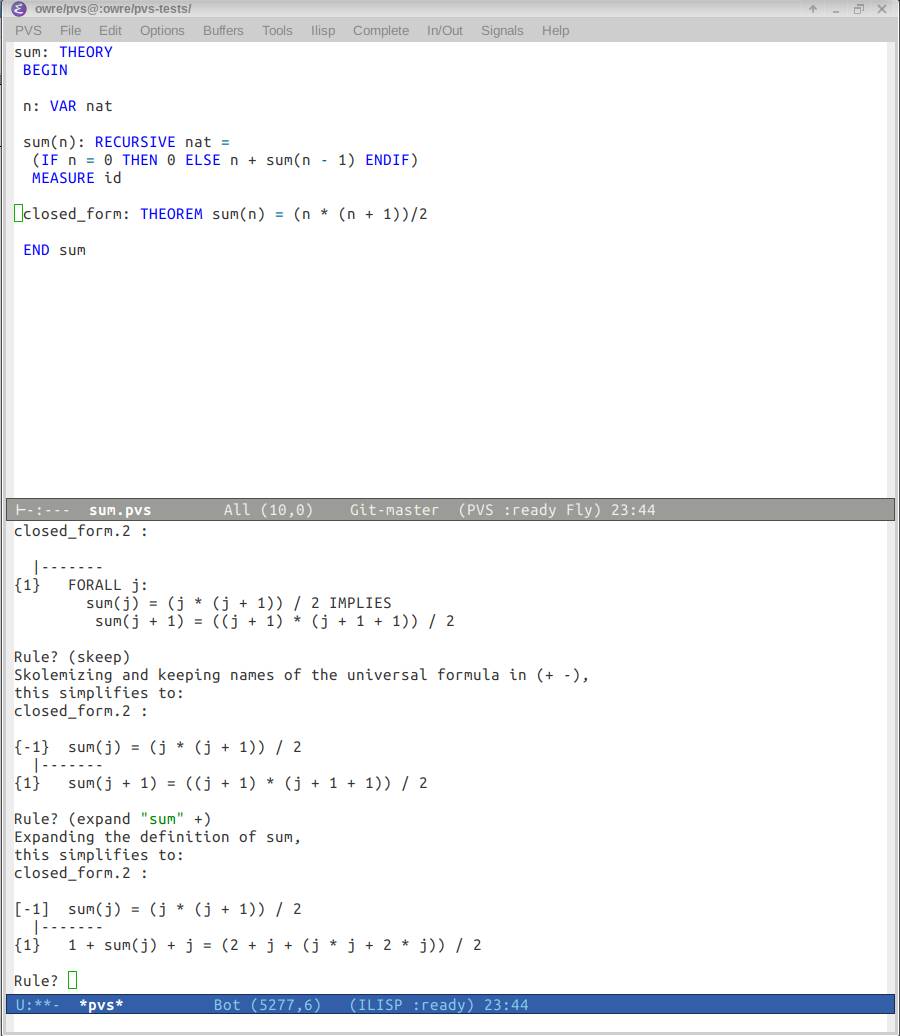
\includegraphics[width=\textwidth]{pvs-screen1.png}
\caption{The \texttt{sum} Specification in Emacs}\label{sum-screen}
\end{figure}

This simple theory has no parameters and contains three declarations.  The
first declares \texttt{n} to be a variable of type \texttt{nat}, the
built-in type of natural numbers.  The next declaration is a recursive
definition of the function \texttt{sum(n)} whose value is the sum of the
first \texttt{n} natural numbers.  Associated with this definition is a
\emph{measure} function, following the \texttt{MEASURE} keyword, which is
explained below.  The final declaration is a formula which gives the
closed form of the sum.

The \texttt{sum} theory may be introduced to the system in a number of
ways, all of which create a file with a \texttt{.pvs}
extension.\footnote{The file does not have to be named \texttt{sum.pvs}, it
simply needs the \texttt{.pvs} extension.}  The most common ways are:
\begin{enumerate}

\item Simply use \texttt{M-x find-file} (\key{C-x C-f}), or \texttt{M-x
find-pvs-file} (\ecmd{ff}, \key{C-c C-f}), provide \texttt{sum.pvs} for
the file name and type in the specification.\footnote{If there is already
a file called \texttt{sum.pvs} in the current context, this will load that
file.}

\item Use the \texttt{M-x new-pvs-file} command (\ecmd{nf}) to create a
new PVS file, and type \texttt{sum} when prompted for a file name.  Then
simply type the specification into the buffer (a basic template will be provided). 

\item Since the file is included in the distribution in the
\texttt{Examples} subdirectory of the main PVS directory, it can be
imported with the \texttt{M-x import-pvs-file} command (\ecmd{imf}).  Use
the \ecmd{whereis-pvs} command to find the path of the main PVS directory.

\item Finally, any external means of introducing a file with extension
\texttt{.pvs} into the current directory will make it available to the
system; for example, going to a \unix\ window and using \texttt{vi} to
type it in, or \texttt{cp} to copy it from the \texttt{Examples}
subdirectory.

\end{enumerate}

\section{Parsing and Typechecking}

Once the \texttt{sum} specification is displayed in the current buffer, it
can be parsed with the \iecmd{parse} (\ecmd{pa}) command, which checks the
syntactic consistency of the specification and creates the internal
abstract representation for the theory described by the specification.  If
the system finds an error during parsing, an error window will pop up with
an error message, and the cursor will be placed in the vicinity of the
error.  If you didn't get an error, introduce one (say by misspelling the
\texttt{VAR} keyword), then move the cursor somewhere else and parse the
file again---note that the buffer is automatically saved.  Fix the error
and parse once more.  In practice, the parse command is rarely used, as
the system automatically parses the specification when it needs to.

\index{typecheck|(}

The next step is to typecheck the file by typing \iecmd{typecheck}
(\iecmd{tc}, \key{C-c C-t}), which checks for semantic errors, such as
undeclared names and ambiguous types.  After \texttt{sum} has been
typechecked, a message is displayed in the minibuffer indicating that two
\tccs\index{TCCs@\tccs|(} were generated.  These \tccs\ represent
\emph{proof obligations}\index{proof obligations} that must be discharged
before the \texttt{sum} theory can be considered typechecked.  The proofs
of the \tccs\ may be postponed indefinitely, though in general it is a
good idea to view \tccs\ to convince yourself that they are provable
before moving on to other proofs in your specification.  \tccs\ can be
viewed using the \iecmd{show-tccs} (\iecmd{tccs}, \key{C-c C-q s})
command, the results of which are shown in Figure~\ref{sum-tccs} below.

\pvstheory{sum-tccs}{\tccs\ for Theory \texttt{sum}}{sum-tccs}

The first \tcc\ is due to the fact that \texttt{sum} takes an argument of
type \texttt{nat}, but the type of the argument in the recursive call to
\texttt{sum} is integer, since \texttt{nat} is not closed under subtraction.
Note that the \tcc\ includes the condition \texttt{NOT n = 0}, which holds
in the branch of the \texttt{IF-THEN-ELSE} in which the expression
\texttt{n - 1} occurs.

The second \tcc\ is needed to ensure that the function \texttt{sum} is
total, \ie\ terminates.  PVS does not directly support partial functions,
although its powerful subtyping mechanism allows PVS to express many
operations that are traditionally regarded as partial.  The measure
function is used to show that recursive definitions are total by requiring
the measure to decrease with each recursive call.

These \tccs\ are trivial, and in fact can be discharged automatically by
using the \ecmd{typecheck-prove} (\ecmd{tcp}) command, which attempts to
prove all \tccs\ that have been generated.  (Try it.)
\index{TCCs@\tccs|)}\index{typecheck|)}

\section{Proving}

We are now ready to try to prove the main theorem.  Place the cursor on
the line containing the \texttt{closed\_form} theorem, and type
\iecmd{prove} (\iecmd{pr} or \key{C-c p}).  A new buffer will pop up, the
formula will be displayed, and the cursor will appear at the
\texttt{Rule?}  prompt, indicating that the prover is ready to accept
input.  The commands needed to prove this theorem constitute only a very
small subset of the commands available to the prover.  In fact, for this
proof all that is actually needed is the single command
\texttt{(induct-and-simplify "n")}, which is a more powerful strategy.
For more information on these and other prover commands consult the prover
guide~\cite{PVS:prover}.

First, notice the display, which consists of a single formula (labeled
\texttt{\{1\}}) under a dashed line.  This is a
\emph{sequent}\index{sequent}; formulas above the dashed lines are called
\emph{antecedents}\index{antecedent} and those below are called
\emph{consequents}\index{consequent}.  The interpretation of a sequent is
that the conjunction of the antecedents implies the disjunction of the
consequents.  Either or both of the antecedents and consequents may be
empty.  An empty antecedent is equivalent to \texttt{true}, and an empty
consequent is equivalent to \texttt{false}, so if both are empty the
sequent is \texttt{false}.  Every proof in PVS starts with a single
consequent.

The basic objective of the proof is to generate a \emph{proof
tree}\index{proof tree} of sequents in which all of the leaves are
trivially true.  The nodes of the proof tree are sequents, and while in
the prover you will always be looking at an unproved leaf of the tree,
called the \emph{current} sequent.\index{current sequent} The
\emph{current} branch\index{current branch} of a proof is the branch
leading back to the root from the current sequent.  When a given branch is
complete (\ie\ ends in a proved leaf), the prover automatically moves on
to the next unproved branch, or, if there are no more unproven branches,
notifies you that the proof is complete.

Now on to the proof.  We will prove this formula by induction on
\texttt{n}.  To do this, type \texttt{(induct "n")}\index{prover
commands!induct@\texttt{induct}}.\footnote{PVS expressions are
case-sensitive, and must be put in double quotes when they appear as
arguments in prover commands.} This is not an Emacs command, rather it
is typed directly at the prompt, including the parentheses.  As indicated,
two subgoals are generated; the one displayed is the base case, where
\texttt{n} is \texttt{0}.  To see the inductive step, type
\texttt{(postpone)}\index{prover commands!postpone@\texttt{postpone}},
which postpones the current subgoal and moves on to the next unproved one.
Type \texttt{(postpone)} a second time to cycle back to the original
subgoal (labeled \texttt{closed\_form.1}).

Three extremely useful Emacs key bindings to know here are \key{M-p},
\key{M-n}, and \key{M-s}.  \key{M-p} gets the last input typed to the
prover; further uses of \key{M-p} cycle back in the input history.
\key{M-n} works in the opposite direction.  To use \key{M-s}, type the
beginning of a command that was previously input, and type \key{M-s}.
This will get the previous input that matches the partial input; further
uses of \key{M-s} will find earlier matches.  Try these key bindings out;
they are easier to use than to explain.  Thus to type the second postpone
command above, you can either type \key{M-p} or type \texttt{(po} followed
by \key{M-s}.  Section~\ref{prover-emacs} on page~\pageref{prover-emacs}
describes further useful shortcut commands for the prover.

To prove the base case, we need to expand the definition of \texttt{sum},
which is done by typing \texttt{(expand "sum")}\index{prover
commands!expand@\texttt{expand}}.  After expanding the definition of
\texttt{sum}, we issue the \texttt{(assert)}\index{prover
commands!assert@\texttt{assert}} command, which applies the decision
procedures of the prover to simplify the consequent to \texttt{TRUE},
completing the proof of this subgoal.  The prover then automatically moves
on to the next subgoal, which is the inductive step.

The first thing to do here is to eliminate the \texttt{FORALL} quantifier.
This can most easily be done with the \texttt{skolem!}\ \index{prover
commands!skolem@\texttt{skolem"!}}  command\footnote{The exclamation point
differentiates this command from the \texttt{skolem} command, where you
provide the new constant names.}, which provides new constants for the
bound variables.  To invoke this command type \texttt{(skolem!)} at the
prompt.  The resulting formula may be simplified by typing
\texttt{(flatten)}\index{prover commands!flatten@\texttt{flatten}}, which
will break up the consequent into a new antecedent and consequent.  The
obvious thing to do now is to expand the definition of \texttt{sum} in the
consequent.  This again is done with the \texttt{expand} command, but this
time we want to control where it is expanded, as expanding it in the
antecedent will not help.  So we type \texttt{(expand "sum" +)},
indicating that we want to expand \texttt{sum} in the
consequent.\footnote{We could also have specified the exact formula number
(here \texttt{1}), but including formula numbers in a proof tends to make
it less robust in the face of changes.  There is more discussion of this
in the prover guide~\cite{PVS:prover}.}

The final step is to invoke the PVS decision procedures, which can
automatically decide certain fragments of arithmetic.  This is done by
typing \texttt{(assert)}. The \texttt{assert}\index{prover
commands!assert@\texttt{assert}} command actually does a lot more than
decide arithmetical formulas, performing three basic tasks:
\begin{itemize}\def\itemsep{0in}
\item It tries to prove the subgoal using the decision procedures.

\item It stores the subgoal information in an underlying database,
allowing automatic use to be made of it later.

\item It simplifies the subgoal by rewriting (if any auto-rewrites have
been given) and by using the underlying decision procedures.
\end{itemize}
These arithmetic and equality procedures are the main workhorses of most
PVS proofs.

The proof is now complete, and is saved in the \texttt{sum.prf} file.  The
buffer from which the \cmd{prove} command was issued is then redisplayed
if necessary, and the cursor is placed on the formula that was just
proved.  The entire proof transcript is shown below.  Yours may be
slightly different, depending on your window size and the timings involved.

{\smaller\smaller
\begin{alltt}
  closed_form :  

    |-------
  \{1\}   FORALL (n: nat): sum(n) = n * (n + 1) / 2

  Rule? (induct "n")
  Inducting on n on formula 1,
  this yields  2 subgoals: 
  closed_form.1 :  

    |-------
  \{1\}   sum(0) = 0 * (0 + 1) / 2

  Rule? (postpone)
  Postponing closed_form.1.

  closed_form.2 :  

    |-------
  \{1\}   FORALL (j: nat):
          sum(j) = j * (j + 1) / 2 IMPLIES sum(j + 1) = (j + 1) * (j + 1 + 1) / 2

  Rule? (postpone)
  Postponing closed_form.2.

  closed_form.1 :  

    |-------
  \{1\}   sum(0) = 0 * (0 + 1) / 2

  Rule? (expand "sum")
  Expanding the definition of sum,
  this simplifies to: 
  closed_form.1 :  

    |-------
  \{1\}   0 = 0 / 2

  Rule? (assert)
  Simplifying, rewriting, and recording with decision procedures,

  This completes the proof of closed_form.1.

  closed_form.2 :  

    |-------
  \{1\}   FORALL (j: nat):
          sum(j) = j * (j + 1) / 2 IMPLIES sum(j + 1) = (j + 1) * (j + 1 + 1) / 2

  Rule? (skolem!)
  Skolemizing,
  this simplifies to: 
  closed_form.2 :  

    |-------
  \{1\}   sum(j!1) = j!1 * (j!1 + 1) / 2 IMPLIES
         sum(j!1 + 1) = (j!1 + 1) * (j!1 + 1 + 1) / 2

  Rule? (flatten)
  Applying disjunctive simplification to flatten sequent,
  this simplifies to: 
  closed_form.2 :  

  \{-1\}  sum(j!1) = j!1 * (j!1 + 1) / 2
    |-------
  \{1\}   sum(j!1 + 1) = (j!1 + 1) * (j!1 + 1 + 1) / 2

  Rule? (expand "sum" +)
  Expanding the definition of sum,
  this simplifies to: 
  closed_form.2 :  

  [-1]  sum(j!1) = j!1 * (j!1 + 1) / 2
    |-------
  \{1\}   1 + sum(j!1) + j!1 = (2 + j!1 + (j!1 * j!1 + 2 * j!1)) / 2

  Rule? (assert)
  Simplifying, rewriting, and recording with decision procedures,

  This completes the proof of closed_form.2.

  Q.E.D.


  Run time  = 0.81 secs.
  Real time = 223.01 secs.

\end{alltt}}

A brief version of the just completed proof can be generated by the command
command \iecmd{show-last-proof}.

\section{Status}

Now type \iecmd{status-proof-theory} (\iecmd{spt}) and you will see a
buffer that displays the three formulas in \texttt{sum}, along with an
indication of their proof status.  This command is useful to see which
formulas and \tccs\ still require proofs.  Another useful command is
\iecmd{status-proofchain} (\ecmd{spc}), which analyzes a given proof to
determine its dependencies.  To use this, go to the \texttt{sum.pvs}
buffer, place the cursor on the \texttt{closed\_form} theorem, and enter
the command.  A buffer will pop up indicating that the proof is
complete, and that it depends on the \tccs\ and the \texttt{nat\_induction}
axiom, as well as some definitions and \tccs\ provided by the prelude.

\section{Generating \LaTeX}

In order to try out this section, you must have access to \LaTeX\
\index{LaTeX@\LaTeX} and a \TeX\ previewer such as
\texttt{xdvi}\index{xdvi}.

Type \iecmd{latex-theory-view} (\iecmd{ltv}).  You will be prompted for
the theory name to which you should type \texttt{sum}, or just
\texttt{Return} if \texttt{sum} is the default.  You will then be prompted
for the \TeX\ previewer name.  Either the previewer must be in your path,
or the entire pathname must be given.  This information will only be
prompted for once per session, after which PVS assumes that you want to
use the same previewer.  You can set the previewer automatically,
by adding the following line to your \texttt{\char'176/.pvsemacs} file.
{\small
\begin{alltt}
\hspace*{2em}  (setq pvs-latex-viewer "\textit{previewer}")
\end{alltt}}

\begin{figure}[ht]
\begin{center}
\begin{boxedminipage}{\textwidth}
{\small\small\input{sum-nosub}}
\end{boxedminipage}
\end{center}
\caption{Theory \texttt{sum} with default translations}\label{sum-plain}
\end{figure}

After a few moments the previewer will pop up displaying the \texttt{sum}
theory, as shown in Figure~\ref{sum-plain}.  Note that \texttt{*} has been
translated as $\times$ and \texttt{LAMBDA} as $\lambda$.  These and other
translations are built into PVS; you may also specify translations for
keywords and identifiers by providing a substitution file named
\texttt{pvs-tex.sub}, that contains commands to customize the \LaTeX\
output.  For example, if the substitution file contains the two lines
{\small\small
\begin{alltt}
    THEORY key 7 \verb|{\large\textbf{\textrm{Theory}}}|
    sum    1   2 \verb|{\sum_{i = 0}^{#1} i}|
\end{alltt}}
\noindent the output will look like Figure~\ref{sum-sub}.  See
Section~\ref{latex-output} on page~\pageref{latex-output} for more
details.

\begin{figure}[t]
\begin{boxedminipage}{\textwidth}
{\small\small% The following substitutions are from the file:
%   /home/owre/pvs.git/pvs-tex.sub
\def\munderscoretimestwofn#1#2{{#1 \times #2}}% How to print function m_times with arity (2)
\def\fmunderscoretimestwofn#1#2{{#1 \times #2}}% How to print function fm_times with arity (2)
\def\sigmaunderscoretimestwofn#1#2{{#1 \times #2}}% How to print function sigma_times with arity (2)
\def\generatedunderscoresubsetunderscorealgebraonefn#1{{{\cal A}(#1)}}% How to print function generated_subset_algebra with arity (1)
\def\generatedunderscoresigmaunderscorealgebraonefn#1{{{\cal S}(#1)}}% How to print function generated_sigma_algebra with arity (1)
\def\aeunderscoredecreasingotheronefn#1{{\pvsid{decreasing?}(#1)~\mbox{\it a.e.}}}% How to print function ae_decreasing? with arity (1)
\def\aeunderscoreincreasingotheronefn#1{{\pvsid{increasing?}(#1)~\mbox{\it a.e.}}}% How to print function ae_increasing? with arity (1)
\def\aeunderscoreconvergenceothertwofn#1#2{{#1 \longrightarrow #2~\mbox{\it a.e.}}}% How to print function ae_convergence? with arity (2)
\def\aeunderscoreeqothertwofn#1#2{{#1 = #2~\mbox{\it a.e.}}}% How to print function ae_eq? with arity (2)
\def\aeunderscoreleothertwofn#1#2{{#1 \leq #2~\mbox{\it a.e.}}}% How to print function ae_le? with arity (2)
\def\aeunderscoreposotheronefn#1{{#1> 0~\mbox{\it a.e.}}}% How to print function ae_pos? with arity (1)
\def\aeunderscorenonnegotheronefn#1{{#1 \geq 0~\mbox{\it a.e.}}}% How to print function ae_nonneg? with arity (1)
\def\aeunderscorezerootheronefn#1{{#1 = 0~\mbox{\it a.e.}}}% How to print function ae_0? with arity (1)
\def\xunderscorelttwofn#1#2{{#1 < #2}}% How to print function x_lt with arity (2)
\def\xunderscoreletwofn#1#2{{#1 \leq #2}}% How to print function x_le with arity (2)
\def\xunderscoreeqtwofn#1#2{{#1 = #2}}% How to print function x_eq with arity (2)
\def\xunderscoretimestwofn#1#2{{#1 \times #2}}% How to print function x_times with arity (2)
\def\xunderscoreaddtwofn#1#2{{#1 + #2}}% How to print function x_add with arity (2)
\def\xunderscorelimitonefn#1{{\pvsid{limit}(#1)}}% How to print function x_limit with arity (1)
\def\xunderscoresumonefn#1{{\sum #1}}% How to print function x_sum with arity (1)
\def\xunderscoresigmathreefn#1#2#3{{\sum_{#1}^{#2} #3}}% How to print function x_sigma with arity (3)
\def\xunderscoresuponefn#1{{\pvsid{sup}(#1)}}% How to print function x_sup with arity (1)
\def\xunderscoreinfonefn#1{{\pvsid{inf}(#1)}}% How to print function x_inf with arity (1)
\def\pointwiseunderscoreconvergesunderscoredowntoothertwofn#1#2{{#1 \searrow #2}}% How to print function pointwise_converges_downto? with arity (2)
\def\pointwiseunderscoreconvergesunderscoreuptoothertwofn#1#2{{#1 \nearrow #2}}% How to print function pointwise_converges_upto? with arity (2)
\def\pointwiseunderscoreconvergenceothertwofn#1#2{{#1 \longrightarrow #2}}% How to print function pointwise_convergence? with arity (2)
\def\convergesunderscoredowntoothertwofn#1#2{{#1 \searrow #2}}% How to print function converges_downto? with arity (2)
\def\convergesunderscoreuptoothertwofn#1#2{{#1 \nearrow #2}}% How to print function converges_upto? with arity (2)
\def\convergenceothertwofn#1#2{{#1 \longrightarrow #2}}% How to print function convergence? with arity (2)
\def\convergencetwofn#1#2{{#1 \longrightarrow #2}}% How to print function convergence with arity (2)
\def\crossunderscoreproducttwofn#1#2{{#1 \times #2}}% How to print function cross_product with arity (2)
\def\conjugateonefn#1{{\overline{#1}}}% How to print function conjugate with arity (1)
\def\cunderscoredivtwofn#1#2{{#1/#2}}% How to print function c_div with arity (2)
\def\cunderscoremultwofn#1#2{{#1\times#2}}% How to print function c_mul with arity (2)
\def\cunderscoresubtwofn#1#2{{#1-#2}}% How to print function c_sub with arity (2)
\def\cunderscorenegonefn#1{{-#1}}% How to print function c_neg with arity (1)
\def\cunderscoreaddtwofn#1#2{{#1+#2}}% How to print function c_add with arity (2)
\def\Imonefn#1{{\Im(#1)}}% How to print function Im with arity (1)
\def\Reonefn#1{{\Re(#1)}}% How to print function Re with arity (1)
\def\Etwofn#1#2{{\mathbb{E}(#1~|~#2)}}% How to print function E with arity (2)
\def\Eonefn#1{{\mathbb{E}(#1)}}% How to print function E with arity (1)
\def\Ptwofn#1#2{{\mathbb{P}(#1~|~#2)}}% How to print function P with arity (2)
\def\Ponefn#1{{\mathbb{P}(#1)}}% How to print function P with arity (1)
\def\xtwofn#1#2{{#1\times#2}}% How to print function x with arity (2)
\def\asttwofn#1#2{{#1\ast#2}}% How to print function ast with arity (2)
\def\minusonefn#1{{{#1}^{-}}}% How to print function minus with arity (1)
\def\plusonefn#1{{{#1}^{+}}}% How to print function plus with arity (1)
\def\astonefn#1{{{#1}^{\ast}}}% How to print function ast with arity (1)
\def\dottwofn#1#2{{#1\bullet#2}}% How to print function dot with arity (2)
\def\integralthreefn#1#2#3{{\int_{#1}^{#2} #3}}% How to print function integral with arity (3)
\def\integraltwofn#1#2{{\int_{#1} #2}}% How to print function integral with arity (2)
\def\integralonefn#1{{\int#1}}% How to print function integral with arity (1)
\def\normonefn#1{{\left||{#1}\right||}}% How to print function norm with arity (1)
\def\phionefn#1{{\pvssubscript{\phi}{#1}}}% How to print function phi with arity (1)
\def\infunderscoreclosedonefn#1{{\left(-\infty,~#1\right]}}% How to print function inf_closed with arity (1)
\def\closedunderscoreinfonefn#1{{\left[#1,~\infty\right)}}% How to print function closed_inf with arity (1)
\def\infunderscoreopenonefn#1{(-\infty,~#1)}% How to print function inf_open with arity (1)
\def\openunderscoreinfonefn#1{(#1,~\infty)}% How to print function open_inf with arity (1)
\def\closedtwofn#1#2{{\left[#1,~#2\right]}}% How to print function closed with arity (2)
\def\opentwofn#1#2{(#1,~#2)}% How to print function open with arity (2)
\def\sigmathreefn#1#2#3{{\sum_{#1}^{#2} #3}}% How to print function sigma with arity (3)
\def\sigmatwofn#1#2{{\sum_{#1} {#2}}}% How to print function sigma with arity (2)
\def\ceilingonefn#1{{\lceil{#1}\rceil}}% How to print function ceiling with arity (1)
\def\flooronefn#1{{\lfloor{#1}\rfloor}}% How to print function floor with arity (1)
\def\absonefn#1{{\left|{#1}\right|}}% How to print function abs with arity (1)
\def\roottwofn#1#2{{\sqrt[#2]{#1}}}% How to print function root with arity (2)
\def\sqrtonefn#1{{\sqrt{#1}}}% How to print function sqrt with arity (1)
\def\sqonefn#1{{\pvssuperscript{#1}{2}}}% How to print function sq with arity (1)
\def\expttwofn#1#2{{\pvssuperscript{#1}{#2}}}% How to print function expt with arity (2)
\def\opcarettwofn#1#2{{\pvssuperscript{#1}{#2}}}% How to print function ^ with arity (2)
\def\indexedunderscoresetsotherIIntersectiononefn#1{{\bigcap #1}}% How to print function indexed_sets.IIntersection with arity (1)
\def\indexedunderscoresetsotherIUniononefn#1{{\bigcup #1}}% How to print function indexed_sets.IUnion with arity (1)
\def\setsotherIntersectiononefn#1{{\bigcap #1}}% How to print function sets.Intersection with arity (1)
\def\setsotherUniononefn#1{{\bigcup #1}}% How to print function sets.Union with arity (1)
\def\setsotherremovetwofn#1#2{{(#2 \setminus \{#1\})}}% How to print function sets.remove with arity (2)
\def\setsotheraddtwofn#1#2{{(#2 \cup \{#1\})}}% How to print function sets.add with arity (2)
\def\setsotherdifferencetwofn#1#2{{(#1 \setminus #2)}}% How to print function sets.difference with arity (2)
\def\setsothercomplementonefn#1{{\overline{#1}}}% How to print function sets.complement with arity (1)
\def\setsotherintersectiontwofn#1#2{{(#1 \cap #2)}}% How to print function sets.intersection with arity (2)
\def\setsotheruniontwofn#1#2{{(#1 \cup #2)}}% How to print function sets.union with arity (2)
\def\setsotherstrictunderscoresubsetothertwofn#1#2{{(#1 \subset #2)}}% How to print function sets.strict_subset? with arity (2)
\def\setsothersubsetothertwofn#1#2{{(#1 \subseteq #2)}}% How to print function sets.subset? with arity (2)
\def\setsothermembertwofn#1#2{{(#1 \in #2)}}% How to print function sets.member with arity (2)
\def\opohtwofn#1#2{{#1\circ#2}}% How to print function O with arity (2)
\def\opdividetwofn#1#2{{\frac{#1}{#2}}}% How to print function / with arity (2)
\def\optimestwofn#1#2{{#1\times#2}}% How to print function * with arity (2)
\def\opdifferenceonefn#1{{-#1}}% How to print function - with arity (1)
\def\opdifferencetwofn#1#2{{#1-#2}}% How to print function - with arity (2)
\def\opplustwofn#1#2{{#1+#2}}% How to print function + with arity (2)
% The following substitutions are from the file:
%   /home/owre/pvs.git/doc/wift95/pvs-tex.sub
\def\sumonefn#1{{\sum_{i = 0}^{#1} i}}% How to print function sum with arity (1)
\begin{alltt}
\pvsid{sum}: \({\large\bf Theory}\)
 \pvskey{BEGIN}

  \(n\): \pvskey{VAR} \(\mathbb{N}\)\vspace*{\pvsdeclspacing}

  \(\sumonefn{n}\): \pvskey{RECURSIVE} \(\mathbb{N}\) \pvskey{=} \pvsid{(}\pvskey{IF} \(n\) \(=\) \(0\) \pvskey{THEN} \(0\) \pvskey{ELSE} \(\opplustwofn{n}{\sumonefn{\opdifferencetwofn{n}{1}}}\) \pvskey{ENDIF}\pvsid{)}
     \pvskey{MEASURE} \pvsid{(}\(\lambda\) \(n\): \(n\)\pvsid{)}\vspace*{\pvsdeclspacing}

  \pvsid{closed\_form}: \pvskey{THEOREM} \(\sumonefn{n}\) \(=\) \(\opdividetwofn{\pvsid{(}\optimestwofn{n}{\pvsid{(}\opplustwofn{n}{1}\pvsid{)}}\pvsid{)}}{2}\)\vspace*{\pvsdeclspacing}

 \pvskey{END} \pvsid{sum}\end{alltt}
}
\end{boxedminipage}
\caption{Theory \texttt{sum} with additional translations}\label{sum-sub}
\end{figure}

\vspace*{1in}

\setcounter{footnote}{0}
% Document Type: LaTeX
% Master File: user-guide.tex
\chapter{PVS Commands}
\label{commands}
\setcounter{footnote}{0}

This chapter contains descriptions for all PVS commands; the commands are
grouped according to function.  A summary of the information in this
chapter is also provided in the buffer displayed by the \ecmd{pvs-help}
command.  The information in this chapter is best absorbed after reading
and experimenting with the brief tour provided in
Chapter~\ref{system-tutorial}.

Each of the following sections begins with a table summarizing the
commands discussed in that section; each table entry gives the full name
of the command, available aliases and/or key bindings, a brief
description, and the effect of providing command arguments.  Commands are
invoked by typing \texttt{M-x} followed by the command name or its
abbreviation, or by using a (less mnemonic) key sequence.  For example,
the \cmd{typecheck} command can be invoked by typing \ecmd{typecheck} or
one of the alternate forms \ecmd{tc} or \key{C-c C-t}.  The behavior of many
of the commands can be modified by providing an argument, and many of the
commands work on regions.\footnote{See Section 4.9 of~\cite{emacs20} for
details on providing arguments to commands, and Section 9 for creating and
manipulating regions.} For example, preceding the \cmd{typecheck} command
with a \key{C-u} or \key{M-1} forces the file to be reparsed and
typechecked, even if it has already been typechecked.  Each command that
takes an argument has a second line prefixed by \emph{Arg:} that
describes the effect of the argument.

Many PVS commands are appropriate at either the file or theory level;
yielding two different commands.  For example, the command for
creating a new PVS file is \cmd{new-pvs-file}, while the command
\cmd{new-theory} creates a template for a new theory within the current
PVS file.  In general, a command \emph{foo} that applies to both
files and theories will have a version named \ecmd{\textit{foo}-pvs-file}
and one named \ecmd{\textit{foo}-theory}.

\section{Exiting PVS}

\begin{pvscmds}
\icmd{exit-pvs} & \key{C-x C-c} & Terminate PVS session \\
\icmd{suspend-pvs} & \key{C-x C-z} & Suspend PVS \\
\end{pvscmds}

The \cmd{exit-pvs} command first saves the context information (see the
\icmd{save-context} command) and then exits PVS\@.  If there is a proof in
progress, the system will not exit, but will instead output a message
asking you to exit the prover, thus giving you the opportunity to save the
proof before exiting.

The \cmd{suspend-pvs} command suspends the Emacs process, except under
X-windows, where the command has no effect.  The system first asks whether
the context should be saved; if you answer \texttt{yes} the
\icmd{save-context} command is invoked prior to suspending PVS.  This may
take a while, as the \cmd{save-context} may have to save any number of
files, depending on what has changed in the context.  The suspended job
can be restarted from the \unix\ shell in which it was suspended by first
determining the job number (using the \unix\ command ``\texttt{jobs}'')
and then typing ``\texttt{fg \%$n$}'', where $n$ is the job
number.\footnote{This assumes you are running the \texttt{csh} or
\texttt{tcsh} shell. To restart under a shell lacking job control, use the
\unix\ command \texttt{ps} to determine the process id ($pid$) and then do
\texttt{kill -CONT pid}.}

\section{Getting Help}
\begin{pvscmds}
\icmd{help-pvs}, \icmd{pvs-help} & \key{C-c h} & Display the PVS help
  buffer \\
\icmd{help-pvs-bnf}, \icmd{pvs-help-bnf} & \key{C-c C-h b} & Display the
  pvs grammar \\
\icmd{help-pvs-language}, & \key{C-c C-h l} & Display help for the PVS
  language \\
\quad\icmd{pvs-help-language} & & \\
\icmd{help-pvs-prover}, & \key{C-c C-h p} & Display help for the prover
  commands \\
\quad\icmd{pvs-help-prover} & & \\
\icmd{help-pvs-prover-command}, & \key{C-c C-h c} &
  Display help for prover command \\
\quad\icmd{pvs-help-prover-command} & & \\
\icmd{help-pvs-prover-strategy}, & \key{C-c C-h s} &
  Displays the specified prover strategy \\
\quad\icmd{pvs-help-prover-strategy} & & \\
\icmd{x-prover-commands} & & Displays the prover commands in a \\
& & \quad Tcl/Tk window \\
\icmd{help-pvs-prover-emacs}, & \key{C-c C-h e} &
  Display help for prover emacs commands \\
\quad\icmd{pvs-help-prover-emacs} & & \\
\icmd{pvs-release-notes}, & \key{C-c C-h r} & Display PVS release notes \\
\end{pvscmds}

The \cmd{help-pvs} command displays a summary of PVS commands in the
\ibuf{PVS Help} buffer.  Help may be obtained for an individual command by
typing \texttt{C-h f} followed by the command or its abbreviation, or by
typing \texttt{C-h k} followed by the key sequence that invokes the
command.  These are built in to Emacs, and may be used to get help for
any Emacs command or key sequence, not just PVS commands.

The \cmd{help-pvs-bnf} command provides the PVS grammar in BNF form, and
the \cmd{help-pvs-language} command displays a summary of the PVS language
with examples in the \ibuf{Language Help} buffer.

The \cmd{help-pvs-prover} command displays the documentation string for
all of the prover commands in the \ibuf{Prover Help} buffer.  The
\cmd{help-pvs-prover-command} displays the documentation string for the
specified command, and the \cmd{help-pvs-prover-strategy} command provides
the arguments, definition, format string, and documentation string for the
specified command.  The latter is useful for finding out exactly what a
strategy does, or for defining your own strategies based on existing ones.
If you are running under the X window system, \icmd{x-prover-commands}
provides an easy interface to get help for individual prover commands.

The \cmd{help-pvs-prover-emacs} command displays a summary of the commands
that provide a convenient Emacs interface to the PVS prover.  This is
discussed in more detail in Section~\ref{prover-emacs},
page~\pageref{prover-emacs}.  The help text appears in the \ibuf{Prover
Emacs Help} buffer.

The \cmd{pvs-release-notes} command displays the release notes for the
running version of PVS.  The text appears in the \ibuf{PVS Release Notes}
buffer.

\section{Editing PVS Files}

\begin{pvscmds}
\icmd{forward-theory} & \key{M-\char125} & Move forward to beginning of next theory \\
\icmd{backward-theory} & \key{M-\char123} & Move backward to beginning of previous theory \\
\icmd{find-unbalanced-pvs} & \key{C-c ]} & Find unbalanced delimiters \\
\icmd{comment-region} & \key{C-c ;} & Comment out all lines in the current region \\
 & & \emph{Arg:} Uncomment all lines in the current region\\
\end{pvscmds}

PVS specification files are edited using the standard Emacs editing
commands.  Appendix~\ref{emacs-intro}, page~\pageref{emacs-intro} gives a
brief introduction to the most useful Emacs commands for editing PVS
files.

The \cmd{forward-theory} and \cmd{backward-theory} commands are used to
move to different theories within a single PVS file.  The cursor is
moved to the beginning of a theory; if there are no preceding or
following theories to move to, the message ``\texttt{No more theories}''
or ``\texttt{No earlier theories}'' is displayed and the cursor remains unchanged.

The \cmd{find-unbalanced-pvs} command checks whether there are any
unbalanced parentheses (\texttt{( )}), square brackets (\texttt{[ ]}), curly
braces (\verb|{ }|), or \texttt{BEGIN-END} pairs.  If none are found, the
message ``\texttt{All delimiters balance}'' is displayed.  Otherwise the
cursor is left at the token for which there is no match and a
corresponding message is displayed.

The \cmd{comment-region} command inserts the comment character
(\texttt{\%}) at the beginning of every line in the specified region.  To
uncomment a region, simply provide an argument to the command, and all
commented lines within the region will be uncommented.

\section{Parsing and Typechecking}

\subsection{Parsing}

\begin{pvscmds}
\icmd{parse} & \icmd{pa} & Parse file in current buffer \\
             & & \emph{Arg:} Forces the file to be reparsed \\
\end{pvscmds}

Parsing a PVS specification accomplishes two things: first, it checks that
the specification is syntactically correct, \ie\ satisfies the PVS
grammar, and second, it builds the internal abstract grammar data
structures.  The \cmd{parse} command is not normally used, as typechecking
will automatically parse the file if required.  Note that only files (with
extension \texttt{.pvs}) may be parsed.  When a file is parsed, it becomes a
part of the context if it wasn't already, and any proofs that have been
saved for the file are reinstated.  If the file being parsed has a valid
\texttt{.bin} file, then this file is loaded instead (this will result in
the file being typechecked as well as parsed).

Parsing is invoked by moving the cursor to a buffer containing a file in
the current context, and issuing the \cmd{parse} command.  While parsing
the file, the minibuffer displays the message ``\texttt{Parsing
\textit{foo}}.''  If there is no error, the message ``\texttt{\textit{foo}
parsed in \textit{\#} seconds}'' is displayed.  If the file has not changed
since the last time it was parsed, the message ``\texttt{\textit{foo} is
already parsed}'' is displayed.  To force reparsing, provide an argument
to the parse command.  Note that the argument is usually not needed, as
changes to the file are automatically detected by the system and the file
is reparsed in that case.

When an error is detected, the file is displayed with the cursor at the
location where the error was detected, which is frequently after the
actual source of the error.  In addition, the \ibuf{PVS Error} buffer is
displayed with an explanatory error message.  You may need to consult the
language manual for details on the grammar.

Certain language features may result in the parser producing theory
messages.  See the \cmd{show-theory-messages} command
(page~\pageref{tc-info}) for details.


\subsection{Typechecking}

\begin{pvscmds}
\icmd{typecheck} & \icmd{tc}, \key{C-c C-t} & Typecheck theories in current buffer \\
& & \emph{Arg:} Force reparsing and retypechecking \\
\icmd{typecheck-importchain} & \icmd{tci} & Typecheck importchain of theories \\
& & \emph{Arg:} Force reparsing and retypechecking \\
\icmd{typecheck-prove} & \icmd{tcp} & Typecheck theories, proving \tccs \\
& & \emph{Arg:} Force reparsing and retypechecking \\
\icmd{typecheck-prove-importchain} & \icmd{tcpi} & Typecheck importchain
of theories,\\ & &  proving \tccs \\
& & \emph{Arg:} Force reparsing and retypechecking \\
\end{pvscmds}

Typechecking a PVS specification checks semantic constraints, determines
the types of expressions, and resolves names (see the language
manual~\cite{PVS:language}).  Typechecking\cmdindex{typecheck} is invoked
much like parsing, and automatically parses the file if necessary.  Errors
are indicated in the same manner as for parsing, although the cursor is
usually more accurately positioned at the error.  As in parsing, an
argument to the command forces reparsing and retypechecking.  Without the
argument, \cmd{typecheck} and \cmd{typecheck-importchain} are the same.
With the argument, \cmd{typecheck} only reparses and retypechecks the
current file, while \cmd{typecheck-importchain} forces reparsing and
retypechecking of the entire import chain of the theories of the current
file.

Forcing a file to be retypechecked is done primarily for development and
debugging, as is the case for reparsing.  If you have typechecked a set of
PVS files, made some changes and found an error on retypechecking that
shouldn't have occurred, try forcing a typecheck of the file where the
error occurred.  If that doesn't help, try forcing with
\cmd{typecheck-importchain}.  The error should disappear after that,
unless it is a true typecheck error.  If it is not a simple typecheck
error, send a bug report to \texttt{pvs-bugs@csl.sri.com}.

The typechecker will attempt to typecheck any theories
appearing in \texttt{IMPORTING} clauses.  If the theories appear in the
current context, then the associated file is typechecked, otherwise
PVS tries to find a file with the same name as the theory.  For
example, in typechecking
\begin{alltt}
  IMPORTING foo[int]
\end{alltt}
the current context (reflected in the context file \texttt{.pvscontext}) is
searched for a file known to contain theory \texttt{foo}.  If no such file is
found, then the file \texttt{foo.pvs} is sought.  If that also cannot be
found, the system complains and the desired file must be manually
located (or created) and typechecked.

The \cmd{typecheck-prove} command typechecks the file, and then attempts
to prove the generated \tccs.  If the file is already typechecked, but the
\tcc\ proofs have not yet been attempted, then they are attempted in the
order they were generated.  The \tcc\ proof attempts are made with 
built-in prover strategies (selected according to the type of \tcc\
generated). These strategies basically expand all
definitions in the \tcc, and repeatedly skolemize, perform heuristic
instantiation, lift \texttt{IF}s, and invoke the decision
procedures.\footnote{The TCC strategies are variants of a powerful
strategy called \texttt{(grind)}, which is useful for more
than just \tccs.} As explained in the prover guide, you may redefine the
\texttt{tcc} strategies; usually to extend their capabilities.

The \cmd{typecheck-prove-importchain} command typechecks the file, and
attempts to prove the \tccs\ of all the theories on the import chain that
have not already been attempted.  Providing an argument forces the
retypechecking of the import chain.

The \cmd{typecheck-prove} commands can take some time, especially if there
are a lot of \tccs.  This can be controlled in a number of ways:
\begin{description}

\item[Use these commands sparingly.] Our experience is that \tccs\ should
be analyzed whenever a new specification is created, significantly
modified, or is nearing completion. 
At these times it pays to use the \cmd{typecheck-prove} command and
to look at the \tccs\ that weren't subsequently proved, and check that
they at least seem provable.
After minor changes, we find it best to use just \cmd{typecheck} and
defer consideration of the \tccs\ until later.


\item[Define your own \tcc\ strategy.] The prover guide describes
techniques for defining your own strategies, and you may change existing
ones, such as the \texttt{tcc} strategy to be more efficient for your
particular specifications.  Changing the \texttt{tcc} strategy should
probably be done in the \texttt{pvs-strategies} file in the current
context, especially if it is tailored to the specifications in that
context.

\item[Use judgements\index{judgements} to cut down on the number of
  \tccs.]  The language manual describes \newline
  how to do this.

\item[Use \texttt{NONEMPTY\_TYPE} or \texttt{CONTAINING} in type
declarations]  This is also described in the language manual.

\end{description}

When typechecking is completed, a message is displayed, indicating the
total number of \tccs\ generated along with a breakdown of the number
proved, subsumed\footnote{A \tcc\ is subsumed if there is an earlier
\tcc\ which implies it.  PVS uses a simple syntactic test, so not all
possible subsumptions will be determined.}, and unproved.

\subsection{Typechecking Information}
\label{tc-info}

\begin{pvscmds}
\icmd{show-theory-warnings} & & Show typechecker warnings for the given theory \\
\icmd{show-pvs-file-warnings} & & Show typechecker warnings for the given file \\
\icmd{show-theory-messages} & & Show typechecker messages for the given theory \\
\icmd{show-pvs-file-messages} & & Show typechecker messagess for the given file \\
\icmd{show-theory-conversions} & & Show conversions for the given theory \\
\icmd{show-pvs-file-conversions} & & Show conversions for the given file \\
\end{pvscmds}

\index{Conversion} \index{typechecker warnings}
\index{typechecker messages}

In the process of typechecking a specification, various warnings and
informative messages may be produced.  These are associated with the
theory that produced them, and saved so they may be perused.  Warnings may
indicate a possible problem.  For example, if the typechecker cannot
determine that a datatype is nonempty, it produces a warning.  There is
nothing wrong with having an empty datatype, but if at some point it isn't
proved to be nonempty, a lot of time may be wasted proving formulas that
are vacuously true.  Informative messages do not indicate anything is
wrong, but the information may be of interest.  For example, using the
\texttt{TYPE+} keyword generates an existence axiom, and this is treated
as an informative message.

Conversion messages\footnote{See the Language Guide\cite{PVS:language} for
details of conversions.} have been separated out of the warnings.
Conversions may be applied to make an expression type correct.  This is
not always what the user intended, so the show conversions commands are
provided to make it easy to look at the conversions that have been applied.

Note that typechecking not only reports the number of \tccs\ generated,
but also the generation of any warnings, messages, and conversions.  While
in the prover, these messages are generated interactively.


\section{Proving}

The prover\index{prover} is described in full in the prover
guide~\cite{PVS:prover}, here we describe the Emacs interface to the
prover, including commands for invoking the prover, editing and rerunning
proofs, displaying proof information, some useful keyboard shortcuts for
the prover, and managing multiple proofs.

The prover may be applied to a single formula, all formulas in a theory,
all formulas in the import chain of a theory, all formulas in a PVS
file, or all formulas in the proof chain of a given formula.  Only the
\cmd{prove}, \cmd{x-prove}, \cmd{step-proof} and \cmd{x-step-proof}
commands lead to prover interaction; the other commands
simply rerun proof scripts that have been previously generated.

PVS keeps track of the status of formulas within and across sessions.  The
status may be one of four values; ``untried'' means that no proof has been
attempted, ``proved'' means that the proof has been completed,
``unchecked'' means that a proof has been completed, but that the
specification has been modified since the proof attempt, and
``unfinished'' means that a proof has been attempted, but not yet
completed.  Formulas labelled as ``proved'' will be ``complete'' or
``incomplete''.  The status is only ``complete'' when all formulas
(including \tccs) upon which the proof is dependent have been completed.

Modifying a specification causes the proof status of all proved formulas
to revert to ``unchecked,'' although the proof scripts are
retained.\footnote{PVS currently tracks the consequences of changes rather
coarsely: any change in a file reverts all the proofs in that file, and
all those in theories that depend on that file (and so on, transitively)
to the ``unchecked'' state.}
\subsection[Proving a Single Formula]{Proving a Single Formula}
\label{prove-commands}

\begin{pvscmds}
\icmd{prove} & \icmd{pr}, \key{C-c p} & Prove formula pointed to by cursor
\\
\icmd{x-prove} & \icmd{xpr}, \key{C-c C-p x} & Start proof along with X
display \\
\icmd{step-proof} & \icmd{prs}, \key{C-c C-p s} & Set up proof stepper for
current formula \\
\icmd{x-step-proof} & \icmd{xsp}, \key{C-c C-p X} & Combines \cmd{x-prove} and \cmd{step-proof} \\
\icmd{redo-proof} & \icmd{prr} \key{C-c C-p r} & Redo the proof of formula at cursor \\
 & & \emph{Arg:} don't display the proof \\
\multicolumn{2}{|l}{
\icmd{prove-next-unproved-formula}} & \\
& \icmd{prnext}, \key{C-c C-p n} & Start proof on next unproved formula
\\
\end{pvscmds}

To invoke the prover on a single formula, move the cursor to any part of
the desired formula and type the \cmd{prove} command.  The formula may be
in a PVS file, a buffer generated by the \cmd{prettyprint-expanded}
command (with extension \ibuf{.ppe}), a buffer generated by the
\cmd{show-tccs} command (with extension \ibuf{.tccs}), or a prelude buffer
produced by one of the \texttt{view-prelude} commands.\footnote{Of course,
the prelude formulas have already been proved; this facility allows you to
explore the proofs.}  If the formula has already been proved, then you
will be asked whether the proof should be retried; a \texttt{no} answer
ends the \cmd{prove} command.  Otherwise, if the formula has an associated
proof script, you will be asked whether to rerun the proof or start over.
In either of these two cases, the proof is displayed in the \ibuf{*pvs*}
buffer.  If the proof script terminates before completing the proof or if
no script was requested, the prover will prompt for a command, which
should be typed directly into the \buf{*pvs*} buffer at the \texttt{Rule?}
prompt.\footnote{The system tries to keep as much of the proof visible as
possible by redisplaying the screen so that the \texttt{Rule?}\ prompt is
at the bottom of the window.  This feature is not always desirable (\eg\
over a slow modem connection), and may be turned off by setting the Emacs
variable \texttt{*pvs-maximize-proof-display*} to nil.}  At this point you
are interacting with the prover, and certain commands will be unavailable
until the prover is exited.\footnote{\label{prover-restrictions}
Specifically, the commands \cmd{parse}, \cmd{typecheck}, \cmd{prove},
\cmd{change-context}, \cmd{exit-pvs}, and all of the prove commands of
this section are unavailable while the prover is active.}

The \cmd{x-prove} command is exactly like the \cmd{prove} command, except
that it also pops up a window in which the proof tree is represented
graphically.  See section~\ref{display-commands},
page~\pageref{display-commands} for more details.  If you are not running
under X windows, then a warning message will be displayed and the command
will be treated as a \cmd{prove} command.

The \cmd{step-proof} command is used to initiate the proof stepper, and is
invoked in the same way as the \cmd{prove} command.  Two buffers are
displayed, one showing the sequent (the \ibuf{*pvs*} buffer) and the other
showing the proof script associated with the formula, if any (the
\ibuf{Proof} buffer).  Section~\ref{proof-stepper},
page~\pageref{proof-stepper} explains how to use the proof stepper.

The \cmd{x-step-proof} command combines the \cmd{x-prove} and
\cmd{step-proof} commands.

The \cmd{prove-next-unproved-formula} command invokes the prover on the
next unproved formula at or beyond the current cursor position.  If the
formula already has a proof, you will be asked whether to go ahead and run
it or to start anew.  Note that starting a new proof will not delete the
old proof unless you allow the prover to overwrite it at the end of the
proof session.

The \cmd{redo-proof} command is invoked exactly like the \cmd{prove}
command, but simply reruns the proof with no questions asked.  An
error is signaled if the indicated formula has no associated proof.
In addition, if an argument is provided, the proof will not be
displayed interactively---instead the proof is processed in the
background, and the status of the proof is provided in the minibuffer
when the attempt is completed.

The prover exits automatically when a proof is successfully completed.  If
at any time you want to exit the prover, go to the bottom of the
\ibuf{*pvs*} buffer\footnote{While in the prover you may freely move
around in the \ibuf{*pvs*} buffer or move to any other buffer to examine
specifications or perform ordinary editing functions.} and type
\texttt{(quit)} to the \texttt{Rule?}\ prompt.  If there is no such
prompt, type \key{C-c C-c} and \texttt{(restore)} to get to the prompt.
Once the prover is exited, control is returned to the buffer from which
the prover was invoked, with the cursor positioned at the beginning of the
formula being proved.  Do not kill the \ibuf{*pvs*} buffer, as
this will also kill the associated PVS process.

\subsection[Proving Sets of Formulas]{Proving Sets of Formulas}
\begin{pvscmds}
\icmd{prove-theory}
  & \icmd{prt}, \key{C-c C-p t}
  & Rerun unproved proofs in theory \\
 & & \emph{Arg:} include those already proved \\
\icmd{prove-theories}
  &
  & Rerun proofs in specified theories \\
 & & \emph{Arg:} include those already proved \\
\multicolumn{2}{|l}{
\icmd{prove-pvs-file}}
  & Rerun unproved proofs in current file \\
 & \icmd{prf}, \key{C-c C-p f}
 & \emph{Arg:} include those already proved \\
\multicolumn{2}{|l}{
\icmd{prove-importchain}}
  & Rerun prove-theory on \texttt{IMPORT} chain \\
 & \icmd{pri}, \key{C-c C-p i}
 & \emph{Arg:} include those already proved \\
\multicolumn{2}{|l}{
\icmd{prove-importchain-subtree}}
  & Rerun prove-theory on specified subtree \\
  & \icmd{pris} & of \texttt{IMPORT} chain \\
 & & \emph{Arg:} include those already proved \\
\multicolumn{2}{|l}{
\icmd{prove-proofchain}}
  & Rerun proofs on formulas in proofchain \\
 & \icmd{prp}, \key{C-c C-p p}
 & \emph{Arg:} include those already proved \\
\multicolumn{2}{|l}{
\icmd{prove-formulas-theory}}
  & Try unproved formulas with specified strategy \\
 & \icmd{prft}
 & \emph{Arg:} attempt proved formulas as well \\
\multicolumn{2}{|l}{
\icmd{prove-formulas-pvs-file}}
 & Try unproved formulas with specified strategy \\
 & \icmd{prff}, \key{C-c C-p U}
 & \emph{Arg:} attempt proved formulas as well \\
\multicolumn{2}{|l}{
\icmd{prove-formulas-importchain}}
 & Try unproved formulas with specified strategy \\
 & \icmd{prfi} & \emph{Arg:} attempt proved formulas as well \\
\multicolumn{2}{|l}{\cmd{prove-formulas-importchain-subtree}\cmdindex{prove-formulas-importchain- \newline subtree}} \\
 & Try unproved formulas with specified strategy \\
 & \icmd{prfs} & \emph{Arg:} attempt proved formulas as well \\
\multicolumn{2}{|l}{
\icmd{prove-tccs-theory}}
  & Try unproved TCCs with specified strategy \\
 & \icmd{prft}
 & \emph{Arg:} attempt proved TCCs as well \\
\multicolumn{2}{|l}{
\icmd{prove-tccs-pvs-file}}
  & Try unproved TCCs with specified strategy \\
 & \icmd{prff}, \key{C-c C-p U}
 & \emph{Arg:} attempt proved TCCs as well \\
\multicolumn{2}{|l}{
\icmd{prove-tccs-importchain}}
 & Try unproved TCCs with specified strategy \\
 & \icmd{prfi} & \emph{Arg:} attempt proved TCCs as well \\
\multicolumn{2}{|l}{
\icmd{prove-tccs-importchain-subtree}}
 & Try unproved TCCs with specified strategy \\
 & \icmd{prfs} & \emph{Arg:} attempt proved TCCs as well \\
\multicolumn{2}{|l}{
\icmd{prove-untried-theory}}
  & Try untried proofs with specified strategy \\
 & \icmd{prut}, \key{C-c C-p u}
 & \emph{Arg:} attempt TCCs as well \\
\multicolumn{2}{|l}{
\icmd{prove-untried-pvs-file}}
  & Try untried proofs with specified strategy \\
 & \icmd{pruf}, \key{C-c C-p U}
 & \emph{Arg:} attempt TCCs as well \\
\multicolumn{2}{|l}{
\icmd{prove-untried-importchain}}
 & Try untried proofs with specified strategy \\
 & \icmd{prui} & \emph{Arg:} attempt TCCs as well \\
\multicolumn{2}{|l}{
\icmd{prove-untried-importchain-subtree}}
 & Try untried proofs with specified strategy \\
 & \icmd{prus} & \emph{Arg:} attempt TCCs as well \\
\end{pvscmds}
Proof scripts can be rerun using the \cmd{prove-theory},
\cmd{prove-pvs-file}, \cmd{prove-importchain},
\cmd{prove-importchain-subtree} and \cmd{prove-proofchain} commands, which
simply rerun the proof scripts, if any, for all of the formulas of the
theory, its PVS file, import chain\index{import chain}, import chain
subtree\index{import chain subtree}, or proof chain\index{proof chain},
respectively.  The import chain of a theory is simply the transitive
closure of the \texttt{IMPORTING}s including those implicit in a theory
declaration.  The \cmd{prove-importchain-subtree} command takes additional
theory name arguments and excludes these theories and their subtree from
the importchain.  The proof chain of a given formula is the transitive
closure of the formulas used in the proof of that formula.  These
commands skip formulas that have no proof scripts, and normally skip
formulas which already have status ``proved;'' providing an argument to
the command forces PVS to reprove all formulas that have proof scripts.
When any of these commands finish processing, the corresponding proof
status command\index{proof status commands} is automatically invoked to
display the results (see Section~\ref{proof-status}).

The \cmd{prove-theories} command prompts for theory names (with
completion) one at a time, until an empty theory name is provided, and
then runs \cmd{prove-theory} on each of these.


The commands
\begin{itemize}\setlength{\topsep}{0pt}\setlength{\parskip}{0pt}%
  \setlength{\itemsep}{0pt}\setlength{\parsep}{0pt}\renewcommand{\labelitemi}{}
\item \cmd{prove-formulas-theory},
\item \cmd{prove-formulas-pvs-file},
\item \cmd{prove-form\-ulas-importchain},
\item \cmd{prove-formulas-importchain-subtree},
\item \cmd{prove-tccs-theory},
\item \cmd{prove-tccs-pvs-file},
\item \cmd{prove-tccs-importchain},
\item \cmd{prove-tccs-importchain-subtree},
\item \cmd{prove-untried-theory},
\item \cmd{prove-untried-pvs-file},
\item \cmd{prove-untried-importchain}, and
\item \cmd{prove-untried-importchain-subtree}
\end{itemize}
are all similar, but allow a
given strategy to be applied to all applicable formulas.

For the \cmd{prove-formulas} commands, all unproved formulas that are not
TCCs or axioms or postulates are attempted with the provided strategy,
which defaults to \texttt{(grind)}.  The \cmd{prove-tccs} commands are
similar, but only attempt unproved TCCs, and the default strategy is
\texttt{(tcc)}.  With an argument, the already proved formulas are also
attempted.  If a given proof attempt succeeds, then it replaces any
existing proof.  If it fails and the given formula already has a proof,
then the original proof is kept.  Otherwise the new proof is associated
with the formula.  Thus after these commands all attempted formulas will
have proofs associated with them.  The strategy is any acceptable single
prover command, as in the following example.
\begin{alltt}
  (then (grind :if-match nil) (inst?) (grind))
\end{alltt}

The \cmd{prove-untried} commands are similar, but they only affect
formulas that have no associated proof, and providing an argument attempts
TCCs that have no proofs as well.  To apply a strategy to just the untried
TCCs, redefine the \texttt{tcc}\index{tcc strategy@\texttt{tcc} strategy}
in your \texttt{pvs-strategies}\index{pvs-strategies file}
Note that after any of these commands,
all attempted formulas will have associated proofs, so issuing the same
command with a different strategy will have no effect.

\glossary{[import chain:] the transitive closure of the \texttt{IMPORTING}s
of a theory}
\glossary{[proof chain:] the transitive closure of the formulas
used in the specified proof}

\subsection{Selecting Decision Procedures}
\label{decision-procedure-commands}

\begin{pvscmdsna}
\multicolumn{2}{|l|}{\icmd{set-decision-procedure}} \\
  & Set the default decision procedure \\
\multicolumn{2}{|l|}{\icmd{prove-theory-using-default-dp}} \\
  & Rerun unproved proofs in specified theory using default decision procedures\\
 & \emph{Arg:} include those already proved \\
\multicolumn{2}{|l|}{\icmd{prove-theories-using-default-dp}} \\
  & Rerun proofs in specified theories using default decision procedures\\
 & \emph{Arg:} include those already proved \\
\multicolumn{2}{|l|}{\icmd{prove-pvs-file-using-default-dp}} \\
 & Rerun unproved proofs in current file using 
  default decision procedures \\
 & \emph{Arg:} include those already proved \\
\multicolumn{2}{|l|}{\icmd{prove-importchain-using-default-dp}} \\
  & Rerun prove-theory on \texttt{IMPORT} chain using
    default decision procedures \\
 & \emph{Arg:} include those already proved \\
\multicolumn{2}{|l|}{\cmd{prove-importchain-subtree-using-default-dp}\cmdindex{prove-importchain-subtree-using- \newline default-dp}} \\
  & Rerun prove-theory on subtree of \texttt{IMPORT}
  chain using default dec. procedures \\
 & \emph{Arg:} include those already proved \\
\multicolumn{2}{|l|}{\icmd{prove-proofchain-using-default-dp}} \\
 & Rerun proofs on all formulas in proof chain using default decision procedures \\
 & \emph{Arg:} include those already proved \\
\end{pvscmdsna}

\emph{These commands have no effect if PVS was invoked with the
\texttt{\textrm{-force-decision-procedures}} switch; see
Section~\ref{invoking-pvs}}

The currently available decision procedures are \texttt{shostak} and
\texttt{ics}.  Much of the prover was built around the Shostak decision
procedure,\footnote{This was developed by Rob Shostak in the late 70s.
Since then it has undergone many refinements.}  ICS is a new decision
procedure that can be run stand alone or included as a library.  See
\url{http://ics.csl.sri.com} for more.  The prover manual discusses how
the decision procedures are used; here we simply describe the commands for
selecting them.

The decision procedure interface provides a set of methods that make it
easy to add new decision procedures, as long as they satisfy the basic
API.  When a new decision procedure is added, it's name is made available
to be used as a decision procedure.

The \cmd{set-decision-procedure} command sets the default decision
procedure to be used in subsequent proofs.  When a single formula is
attempted that doesn't have a proof, the default decision procedure is
automatically used.  If it already has a proof that was developed using
a different decision procedure, the prover prompts for whether to use the
default or stay with the original decision procedure.  When a proof is
saved, the decision procedure used during the proof is saved as well.  For
the prover commands such as \cmd{prove-theory}, the proofs are each
attempted with the decision procedure they were developed with.  The
remaining commands allow existing proofs to be rerun using the default
decision procedures, and otherwise behave exactly as the similarly named
commands defined in the previous section.

Note that setting the decision procedure does not affect an ongoing
proof.  The decision procedures generally have different ways of storing
state and processing it, and a proof may only be run with a single
decision procedure.  However, the decision procedure API is flexible
enough to allow methods to be defined that, for example, run two different
decision procedures in parallel and compare their results, or spawn two
subprocesses and use the result of the first one to finish.

\subsection{Editing and Viewing Proofs}

\begin{pvscmds}
\icmd{edit-proof} & \icmd{show-proof} & Edit the proof of the indicated
formula \\
\icmd{install-proof} & \key{C-c C-i} & Install proof on the indicated formula \\
\icmd{install-and-step-proof} & \key{C-c s} & Install proof on a formula and step \\
\icmd{install-and-x-step-proof} & \key{C-c x} & Install proof on formula, display, and step \\
\icmd{remove-proof} & & Remove proof associated with a formula \\
\icmd{show-proof-file} & & Edit the proofs of the indicated PVS file \\
\icmd{show-orphaned-proofs} & & Edit the orphaned proofs \\
\icmd{show-proofs-theory} & & Show all proofs of a theory \\
\icmd{show-proofs-pvs-file} & & Show all the proofs of a PVS file \\
\multicolumn{2}{|l}{\icmd{show-proofs-importchain}} & Show all proofs of importchain of
a theory \\
\multicolumn{2}{|l}{\icmd{install-pvs-proof-file}} & Installs proof file
for typechecked theory \\
\icmd{display-proofs-formula} & & Display the (multiple) proofs associated
with this formula \\
\icmd{display-proofs-theory} & & Display the (multiple) proofs of the
formulas in the theory \\
\icmd{display-proofs-pvs-file} & & Display the (multiple) proofs of the
formulas in the PVS file \\
\icmd{load-pvs-strategies} & & Loads a pvs-strategies file \\
\icmd{set-print-depth} & & Sets print depth for printing sequents \\
\icmd{set-print-length} & & Sets print length for printing sequents \\
\icmd{set-print-lines} & & Sets number of lines to print \\
 & & \quad for each sequent formula \\
\icmd{set-rewrite-depth} & & Sets the print depth for rewrite messages \\
\icmd{set-rewrite-length} & & Sets the print length for rewrite messages \\
\icmd{dump-sequents} & & Save unproved sequents to a file \\
\multicolumn{2}{|l}{\icmd{toggle-proof-prettyprinting}} & Toggles the prettyprinting of proof
files \\
\end{pvscmds}

Every formula of a specification for which a proof has been attempted has
an associated proof script that reflects the commands used during the
proof attempt.  Proof scripts may be edited using the \cmd{edit-proof}
command.  This command is invoked on the formula declaration at the
cursor; the formula may occur in a specification buffer (with extension
\ibuf{.pvs}), a prettyprint-expanded buffer (with extension \ibuf{.ppe}),
a show-tccs buffer (with extension \ibuf{.tccs}), or a buffer generated by
one of the \texttt{view-prelude} commands.  When the \cmd{edit-proof}
command is invoked, it creates a buffer with the name \ibuf{Proof}
containing the relevant proof script,\footnote{If the formula has no proof
script, an empty \ibuf{Proof} buffer is created.}  which may then be
edited using the standard Emacs editing commands.  Editing proof scripts
is a convenient way to handle modifications made to a specification, and
allows the same proof script to be revised and used for many similar
formulas.  The \ibuf{Proof} buffer normally persists until the next time
the \cmd{edit-proof} command is invoked, allowing the same proof script to
be attached to different formulas using \icmd{install-proof}.

A proof script records a tree of prover commands that will generate a
proof of the given formula.  Although the proof tree does not record
verbatim the commands originally typed to the prover, the proof script
should be easy to understand.  For example, the \ibuf{Proof} buffer of
the formula \texttt{closed\_form} in the \texttt{sum} example would
contain

{\small\small
\begin{alltt}
  ;;; Proof for formula sum.closed_form
  ;;; developed with old decision procedures
  (""
   (INDUCT "n")
   (("1" (EXPAND "sum") (ASSERT))
    ("2" (SKOLEM!) (FLATTEN) (EXPAND "sum" +) (ASSERT))))
\end{alltt}}

When editing is complete, the proof script may be attached either to the
original, or to a different formula using the \cmd{install-proof} command.
If this command is invoked in the \ibuf{Proof} buffer, it attaches the new
proof script to the original formula and offers to rerun the proof.  The
proof script may also be attached to any other formula by invoking
\cmd{install-proof} in a \ibuf{.pvs}, \ibuf{.ppe}, or \ibuf{.tccs} buffer,
in which case the script is attached to the formula at the cursor.  In
each case, the new proof only becomes the default, the old proofs are
still available and may be manipulated by means of the
\cmd{display-proofs-formula} command, which allows the default proof to be
reset.  If no proof is being edited (\ie\ there is no \ibuf{Proof}
buffer), an error is reported.

The proof may also be installed using the \cmd{install-and-step-proof} or
\cmd{install-and-x-step-proof} commands, both of which install the proof
and initiate the proof stepper; the latter also displays the proof tree.

Checkpoints may be added to the \texttt{Proof} buffer obtained by the
\texttt{edit-proof} command.  To add a checkpoint, position the cursor and
type \texttt{C-c a}.  The checkpoint is indicated by a double exclamation
point (\texttt{!!}).  Any number of checkpoints may be added.  When the
proof is installed using \texttt{C-c C-i}, these are changed to the
\texttt{checkpoint} proof rule, and branches of the proof that do not have
a checkpoint on them are wrapped in a \texttt{just-install-proof} proof
rule.  When this proof is rerun, it will run until it hits a
\texttt{checkpoint}, and then prompt for a prover command.  When it hits a
\texttt{just-install-proof}, it simply installs the given commands and
marks that branch as proved.  This allows the prover to quickly get to the
next checkpoint, without attempting to reprove branches that do not have
checkpoints in them.  When a proof that has \texttt{just-install-proof}
rules in it is finished, the prover asks whether the proof should be
rerun, as the formula will not be considered proved until the proof is
rerun.

To remove a checkpoint from the \texttt{Proof} buffer, position the cursor
at the checkpoint and type \texttt{C-c r}.  To remove all checkpoints,
type \texttt{C-c DEL}.

In addition to the above, the key bindings for browsing and the prover
emacs (\textsc{tab}) commands are available in a \texttt{Proof} buffer.

The \cmd{remove-proof} command is used to remove the proof associated with
the specified formula.  The primary use for this is to remove proofs from
axioms for which a proof attempt has been made.

If a proof is in progress, proofs may still be edited, but the prover must
be exited before the edited proof may be attached to a formula.  Note that
invoking \icmd{edit-proof} on the formula currently being proved will
display the proof script stored with the formula, if there is one.  To
display the current proof script, use the \icmd{show-current-proof}
command described below.

As noted above, each specification file (with extension \texttt{.pvs}) has
an associated proof file of the same name with a \texttt{.prf} extension.
This file contains the proof scripts for all of the formulas of the
specification file whose proofs have been attempted.  The
\cmd{show-proof-file} command allows you to browse a proof file, and
select or view any of the associated proof scripts.  A \ibuf{Proofs File}
buffer is created with a line for each proof script in the file.  You may
select a proof script for editing, or simply view the script in a pop-up
buffer.  This command may be used to look at the proof file of any context
or PVS file---in this respect it is analogous to the \cmd{import-pvs-file}
command.

To view a proof script, place the cursor on the desired line, and type
``\texttt{v}.''  The proof script will be displayed in a pop-up buffer,
but may not be edited.  To edit a proof script, position the cursor and
type ``\texttt{s}.''  This will create or use the \ibuf{Proof} buffer
which may be edited and attached to formulas exactly as described above.

While developing a specification, some theorems or even entire theories
may be moved around or deleted, creating \emph{orphaned}
proofs\index{orphaned proofs}.  Orphaned proofs are saved in the
\texttt{orphaned-proofs.prf} file.  In some cases,
the system will recognize that an orphaned proof should be reattached to a
formula, and will ask whether it should go ahead.

The \cmd{show-orphaned-proofs} command provides access to the orphaned
proofs file by means of an \ibuf{Orphaned Proofs} buffer that displays the
formula name, theory name, and file name associated with each orphaned
proof.  A given proof may be selected by moving the cursor to the line and
typing ``\texttt{s},'' which pops up the \ibuf{Proof} buffer.  This buffer
is the same as the one generated by the \cmd{edit-proof} command, except
that there is no default formula, so that \cmd{install-proof} (\key{C-c
C-i}) will not work from the \ibuf{Proof} buffer.  Typing a ``\texttt{d}''
on a proof line deletes the corresponding entry from the orphaned proof
file, typing a ``\texttt{v}'' pops up a \ibuf{View Proof} buffer, and
typing a ``\texttt{q}'' exits the orphaned proof buffer.

The commands \cmd{show-proofs-theory}, \cmd{show-proofs-pvs-file}, and
\cmd{show-proofs-importchain} display all of the proofs of the associated
theory, PVS file, or importchain in a buffer named \ibuf{Show Proofs},
which is in \texttt{PVS View} mode.

The \cmd{install-pvs-proof-file} command prompts for a PVS file name, and
reads in the corresponding proof file, replacing any proofs that may have
been loaded or developed.  This command is needed in order to get a new
proof file accepted in a context.  When specification files are parsed
and/or typechecked, the corresponding proof files are read in.  After that
the system will not pay any attention to changes made to the proof file,
but simply update it as changes are made that affect proof status.  This
command allows you to modify the file or copy a new one in and get it
installed.

The \cmd{load-pvs-strategies} command loads the strategies files from your
home directory, imported libraries, and the current context.  This command
is only needed when a new strategy is being developed during a proof; when
a proof is started the system checks whether any of the strategy files
have changed and automatically loads them if they have.  See the prover
guide~\cite{PVS:prover} for details on the contents of the
\texttt{pvs-strategies}\index{pvs-strategies file} files.

The \cmd{set-print-depth}, \cmd{set-print-length}, and
\cmd{set-print-lines} commands control how much of an expression is
displayed in a sequent.  If the print depth and length are set to 0 and
the lines is \texttt{NIL}, then the entire sequent is displayed.  This is
the default.  If the depth is set to a positive integer, then any subterms
at that depth are replaced by a pound sign (\texttt{\#}).  Similarly, if
the length is set to a positive integer, then any subterms beyond the
specified length are replaced by three periods (\texttt{...}).  The length
and depth of an expression are not easy to define, because it is related
to the abstract syntax used by the prettyprinter.  In general, expressions
separated by commas have a length, while subterms\footnote{For example,
the operator and arguments are subterms of an application.} are deeper by
one than the containing terms.  If the print lines is set to a number $n$,
then only the first $n$ lines of each formula of the sequent is displayed,
and remaining lines are replaced by two periods (\texttt{..}).  Note that
all these commands are also rules in the prover that otherwise behave as a
\texttt{SKIP}, so it is easy to adjust the printout interactively.

The \cmd{set-rewrite-depth} and \cmd{set-rewrite-length} commands control
how much information to output when printing the results of automatic
rewrites.  Normally, both the rule name and the expression being rewritten
are displayed in the proof commentary when an auto-rewrite is triggered.
The value should be a positive number or \texttt{NIL}.  If it is a
positive number, then any subexpression at that depth or length will be
replaced by a pair of periods (\texttt{..}) or three periods
(\texttt{...}) respectively.  If it is 0 (zero), then only the rule name
is displayed.  If it is \texttt{NIL}, then there is no bound.

The \cmd{dump-sequents} command indicates that any incomplete proof
attempt should save the remaining unproved sequents to file.  If the proof
is for formula \texttt{foo} from theory \texttt{th}, then the file
containing the unproved sequents is named \texttt{th-foo.sequents}.  If
the formula is proved, then no file is generated, and any file left from
an earlier attempt on this formula is removed.

The \cmd{toggle-proof-prettyprinting} command toggles whether to
prettyprint the proof file (with extension .prf) associated with a PVS
file.  Prettyprinted files are easier to read, edit, and email, but they
take a lot longer to generate.  By default, proof files are prettyprinted.

The commands for exhibiting proofs can get confusing.  In short,
only the \cmd{display-proofs-} commands support multiple proofs, while the
others just show the default proofs.  The \cmd{show-proof-file} 
and \cmd{show-orphaned-proofs} commands provide listings that are similar
to those produced by the \cmd{display-proofs-} commands, but without the
ability to set the default proof.

\subsection{Displaying Proof Information}

\begin{pvscmdsna}
\icmd{show-current-proof} & Display the current proof \\
\icmd{show-last-proof} & Displays printout of most recent proof\\
 & \emph{Arg:} make it brief\\
\icmd{set-proof-backup-number} & Set number of backup proof files to
retain\\
& \emph{Arg:} number of files to retain\\
\icmd{show-proof-backup-number} & Show number of backup proof files 
retained\\
\icmd{ancestry} & Display the ancestry of the current sequent \\
\icmd{siblings} & Display the siblings of the current sequent \\
\icmd{show-hidden-formulas} & Display the hidden formulas in the
current sequent \\
\icmd{show-auto-rewrites} & Display the currently used auto-rewrite
rules \\
\icmd{show-expanded-sequent} & Display the sequent in expanded form \\
 & \emph{Arg:} also expand names from the prelude \\
\icmd{show-skolem-constants} & Display the Skolem constants and their
types \\
\icmd{explain-tcc} & Display the explanation for a TCC \\
\icmd{usedby-proofs} & Display formulas whose proofs refer to the \\
 & declaration at the cursor \\
\icmd{pvs-set-proof-parens} & Control parentheses display in proofs \\
\icmd{pvs-set-proof-prompt-behavior} & Indicates the kind of prompting at
the end of a proof;\\
 & one of \texttt{:ask}, \texttt{:overwrite}, or
\texttt{:new} \\
\icmd{pvs-set-proof-default-description} & Sets a default description
string for saved proofs \\
\end{pvscmdsna}

These commands work only while an interactive proof is being developed,
\ie\ after the \cmd{prove} command.  The \cmd{show-current-proof} command
shows the current proof in the \ibuf{*Proof*} buffer in the same format as
the \cmd{edit-proof} command, but the displayed proof may not be edited.
The primary use of this facility is for reviewing the development of a
proof in progress and applying parts of it to other branches using the
\texttt{rerun} prover command, as described in the prover guide\cite{PVS:prover}.

%\memo{Is the cut and paste proof command documented yet?}

The \cmd{show-last-proof} command provides a display of the commentary and
subgoals associated with the most recently completed proof in the
\ibuf{Proof Display} buffer.  This version does not contain the
\texttt{undo}, \texttt{skip}, or \texttt{postpone} steps and provides a
clean version that shows the commentary and subgoals.  This printout is
useful in trying to summarize the proof for publication.  With an
argument, many of the sequents are suppressed, and within a sequent,
formulas which haven't changed since the previous sequent display are
elided.

\label{proof-backups}
The \cmd{set-proof-backup-number} command indicates the number of
backups to be kept for proof files.  If the argument is 0, then
no backups are kept.  If it is 1, then before the {\tt .prf} file is
written, the old copy is retained with extension {\tt .prf\char'176}.
For larger arguments, that number of old {\tt .prf} files are retained with the
extension {\tt .prf.\char'176x\char'176}, with increasing values of {\tt
x}.  For example, if the argument is 3, and backup files
{\tt foo.prf.\char'176{3}\char'176}, 
{\tt foo.prf.\char'176{4}\char'176}, and
{\tt foo.prf.\char'176{5}\char'176} exist, when the next backup
is created {\tt foo.prf.\char'176{3}\char'176} is removed and
{\tt foo.prf.\char'176{6}\char'176} is created.  The default value
is 1, and PVS will revert to this behaviour on each invocation.  Thus,
it is recommended that this command be placed in the file {\tt .pvsemacs}
in your home directory, e.g.:
\begin{alltt}
(set-proof-backup-number 5)
\end{alltt}
The current number of proof files being retained is reported
by the \cmd{show\-proof-backup-number} command.

The \cmd{ancestry} command displays the branch of the proof from the root
to the current sequent in the \ibuf{Ancestry} buffer, and the
\cmd{siblings} command displays the siblings of the current sequent in the
\ibuf{Siblings} buffer, where the siblings are those sequents of the proof
tree which share the same parent.

The \cmd{show-hidden-formulas} command displays the formulas that have
been hidden in the current branch of the proof.  These formulas are
displayed in the \ibuf{Hidden} buffer.  Each formula is displayed with a
number which may be referred to in the \cmd{reveal} prover command (see
the prover guide~\cite{PVS:prover}).

The \cmd{show-auto-rewrites} command displays the auto-rewrite rules that
are in effect for the current sequent.  The rules are displayed in the
\ibuf{*Auto-Rewrites*} buffer, in reverse of the order in which they were
introduced \ie\ the most recently introduced ones first.  The order is
significant since if there is a clash and two or more rewrite rules are
applicable, the most recently introduced one is applied first.

The \cmd{show-expanded-sequent} command displays the current sequent in
the \ibuf{Expanded Sequent} buffer, with each variable, constant and
operator expanded to its full type, including the theory and its
parameters, unless they are from the current theory or the prelude.  With
an argument, prelude names are also expanded. \cmd{show-skolem-constants}
displays the type of all skolem constants introduced in the current proof
in the \ibuf{Proof Display} buffer.  Normally names from the prelude are
not expanded, an argument expands these as well.

A \tcc\ subgoal is marked as such in a proof. Invoking the
\cmd{explain-tcc} command provides some explanation for why the \tcc\ was
generated, giving the type of \tcc, and the expression which caused its
generation.

The \cmd{usedby-proof} command provides a list of formulas whose proofs
refer to the given declaration.  This works by looking through the
formulas of all the currently typechecked theories of the current context;
in particular, for prelude or library declarations it will not locate all
formulas that ever referred to the declaration, as this information would
be difficult to maintain and be of marginal use.  The buffer generated by
the \cmd{usedby-proof} command is the same as that for the
\cmd{find-declaration} command, with the same key-bindings for viewing and
going to the listed declarations.

The \cmd{pvs-set-proof-parens} command asks whether to show parentheses,
and if so, sets a variable indicating that sequents should be displayed
with full parenthesization.  This is mostly useful for proofs involving
large arithmetic terms, where it may otherwise be difficult to figure out
whether a given rewrite rule should apply.

The introduction of multiple proofs changed the way PVS handles the end of
a proof session.  When a proof attempt is ended, either by quitting or
successfully completing the proof, the proof is checked for changes.  If
any changes have occured, the user is queried about whether to save the
proof, and whether to overwrite the current proof or to create a new
one.  If a new proof is created, the user is prompted for a proof
identifier and a description.  At the end of any given proof a number of
questions may be asked:
\texttt{
\begin{itemize}
\item Would you like the proof to be saved?
\item Would you like to overwrite the current proof?
\item Please enter an id
\item Please enter a description:
\end{itemize}}
The \cmd{pvs-set-proof-prompt-behavior} command allows you to control this
behavior.  The possible values for the prompt behavior are:

\begin{tabular}{rp{11cm}}
  \texttt{:ask} & the default; all four questions are asked \\
  \texttt{:overwrite} & similar to earlier PVS versions; asks if the proof
                        should be saved and then simply overwrites the
                        earlier one \\ 
  \texttt{:add} & asks if the proof should be saved, then creates a new
                  proof with a generated id and empty description.
\end{tabular}

The \cmd{pvs-set-proof-default-description} command allows you to set a
default description string.  It is used if the prompt is anything but
\texttt{:ask}, or if the empty string (i.e., just hitting Return) is
provided when a description is asked for.  It defaults to the empty
string.

\subsection{Adding and Modifying Declarations}
\label{add-decl}

\begin{pvscmds}
\icmd{add-declaration} & & Add declarations to a PVS theory \\
\icmd{modify-declaration} & & Modify the indicated declaration body \\
\end{pvscmds}

Declarations are normally added and modified directly in a specification
buffer; the system determines the differences and updates the
corresponding internal structures accordingly.  This can be quite
expensive, as any theories which import a modified theory must be
retypechecked.  However, there are two commands that allow
declarations to be added and modified without causing retypechecking.
This is especially important during proof development, when these
commands allow you to make adjustments to theories precisely when
the need for such an adjustment is discovered.

The \cmd{add-declaration} command inserts new declarations before the
declaration at the cursor.  When invoked, it pops up an empty buffer named
\ibuf{Add Declaration}.  Declarations may be typed in and edited just as
in a specification buffer.  When editing is completed, the new
declarations may be installed by typing \key{C-c C-c}.  The new
declarations are parsed, typechecked, and checked for uniqueness; if an
error is discovered it is reported in the usual way.  If there is no
error, the declarations are inserted above the declaration located at the
cursor when the \cmd{add-declaration} command was invoked.  If a proof is
in progress, it will have access to the new declarations if they are
visible, \ie\ exported,\footnote{See the Language Reference for a
definition of exported declarations.  In short, formal parameters and
variable declarations may never be exported, and, by default, everything
else is exported.} declarations of a theory used by the theory whose
formula is being proved, or they occur in the same theory and precede the
formula being proved.

The \cmd{modify-declaration} command is used to modify the body of a
constant or formula declaration; modifying the signature of a constant or
any other kind of declaration is not permitted because these modifications
have potentially non-local ramifications.  This command is similar to the
\cmd{add-declaration} command: the \ibuf{Modify Declaration} buffer pops
up containing the declaration at the cursor, and the modified declaration
is installed by typing \key{C-c C-c}.  If the modified declaration
typechecks and maintains the same id and signature, it is installed in the
theory and is immediately available for use in a proof.  Otherwise the
cursor is placed in the vicinity of the error and a message is displayed
indicating the nature of the error.

Both \cmd{add-declaration} and \cmd{modify-declaration} update the buffer
containing the affected theory and mark the buffer as unchanged; the
system considers the affected theory typechecked.  However, the checks
cannot guarantee that everything is sound; for example, any proofs done
using a declaration that was later modified will need to be reproved, and
any theory which uses a theory to which declarations have been added
should eventually be retypechecked, as ambiguities may have inadvertently
been introduced.  Thus these commands should be viewed as a convenient way
to explore proofs; they should not be used in the ``validation'' phase of
the verification.  Proofs constructed when either of these commands is
successfully used are marked unchecked; \ie\ the proofs will need to be
rerun to change their status to proved.


\subsection{Prover Emacs Commands}
\label{prover-emacs}

The prover commands can be somewhat tedious to type in, especially the
simple ones that are used regularly, such as \texttt{assert},
\texttt{grind} and \texttt{skosimp*}.  C. Michael Holloway of NASA Langley
created an extension to Emacs to relieve some of the tedium, and was kind
enough to make these extensions available to PVS.  This section describes
those extensions in three subsections: General Commands, Prover Commands,
and Proof Stepper Commands.

\subsection{General Commands}
\begin{pvscmds}
\icmd{pvs-prover-any-command} & \key{TAB TAB} & Insert (prompted for) command \\
\icmd{pvs-prover-quotes} & \key{TAB '} & \\
\icmd{pvs-prover-wrap-with-parens} & \key{TAB C-j} & \\
\end{pvscmds}

The \cmd{pvs-prover-any-command} prompts for a command (with completion),
and inserts it in the prover buffer with the cursor positioned for
additional arguments.  This command is provided for those prover commands that do
not have an Emacs key binding associated with them.

The \cmd{pvs-prover-quotes} command makes it easier to give PVS types and
expressions, by inserting a pair of double quotes around the current
cursor location.  The \cmd{pvs-prover-wrap-with-parens} command wraps a
given prover command in parentheses and send it to the prover.  You must
be at the end of the prover input to use this command.

\subsection{Prover Commands}

These commands simply prompt for any arguments, and then apply the
specified prover command to those arguments.  After all the arguments, if
any, have been given the command is immediately executed by the prover.
Not all prover commands are represented below, and even for those that are
given below not all arguments are prompted for.  Commands with complex
arguments are generally easier to type in directly, using the
\ecmd{pvs-prover-any-command} command if desired.  The \key{M-p},
\key{M-n}, and \key{M-s} keys are particularly useful in this case, as a
mistyped prover command can easily be brought back and corrected, or a
complex command that is used frequently may be easily brought back.

The prover command associated with the following Emacs commands should be
obvious.  Details for any given command may be found by typing \key{C-h d}
followed by the command name, e.g., \texttt{pvs-prover-auto-rewrite}.

\begin{pvscmds}
\icmd{pvs-prover-apply-extensionality} & \key{TAB E} & \\
\icmd{pvs-prover-assert} & \key{TAB a} &  \\
\icmd{pvs-prover-auto-rewrite} & \key{TAB A} &  \\
\icmd{pvs-prover-auto-rewrite-theory} & \key{TAB C-a} & \\
\icmd{pvs-prover-bddsimp} & \key{TAB B} & \\
\icmd{pvs-prover-beta} & \key{TAB b} & \\
\icmd{pvs-prover-case} & \key{TAB c} & \\
\icmd{pvs-prover-case-replace} & \key{TAB C} & \\
\icmd{pvs-prover-decompose-equality} & \key{TAB =} & \\
\icmd{pvs-prover-delete} & \key{TAB d} & \\
\icmd{pvs-prover-do-rewrite} & \key{TAB D} & \\
\icmd{pvs-prover-expand} & \key{TAB e} & \\
\icmd{pvs-prover-extensionality} & \key{TAB x} & \\
\icmd{pvs-prover-flatten} & \key{TAB f} & \\
\icmd{pvs-prover-grind} & \key{TAB G} & \\
\icmd{pvs-prover-ground} & \key{TAB g} & \\
\icmd{help-pvs-prover-command} & \key{TAB H} & \\
\icmd{pvs-prover-hide} & \key{TAB C-h} & \\
\icmd{pvs-prover-iff} & \key{TAB F} & \\
\icmd{pvs-prover-induct} & \key{TAB I} & \\
\icmd{pvs-prover-induct-and-simplify} & \key{TAB C-s} & \\
\icmd{pvs-prover-inst} & \key{TAB i} & \\
\icmd{pvs-prover-inst-question} & \key{TAB ?} & \\
\icmd{pvs-prover-lemma} & \key{TAB L} & \\
\icmd{pvs-prover-lift-if} & \key{TAB l} & \\
\icmd{pvs-prover-model-check} & \key{TAB M} & \\
\icmd{pvs-prover-musimp} & \key{TAB m} & \\
\icmd{pvs-prover-name} & \key{TAB n} & \\
\icmd{pvs-prover-postpone} & \key{TAB P} & \\
\icmd{pvs-prover-prop} & \key{TAB p} & \\
\icmd{pvs-prover-quit} & \key{TAB C-q} & \\
\icmd{pvs-prover-replace} & \key{TAB r} & \\
\icmd{pvs-prover-replace-eta} & \key{TAB 8} & \\
\icmd{pvs-prover-rewrite} & \key{TAB R} & \\
\icmd{pvs-prover-skolem-bang} & \key{TAB \char033} & \\
\icmd{pvs-prover-skosimp} & \key{TAB S} & \\
\icmd{pvs-prover-skosimp-star} & \key{TAB *} & \\
\icmd{pvs-prover-split} & \key{TAB s} & \\
\icmd{pvs-prover-tcc} & \key{TAB T} & \\
\icmd{pvs-prover-then} & \key{TAB C-t} & \\
\icmd{pvs-prover-typepred} & \key{TAB t} & \\
\icmd{pvs-prover-undo} & \key{TAB u} & \\
\end{pvscmds}

\subsection{Proof Stepper Commands}
\index{proof stepper|(}
\label{proof-stepper}

\begin{pvscmds}
\icmd{pvs-prover-one-proof-step} & \key{TAB 1} & \\
\icmd{pvs-prover-many-proof-steps} & \key{TAB \char064} & \\
\icmd{pvs-prover-undo-one-proof-step} & \key{TAB U} & \\
\icmd{pvs-prover-undo-many-proof-steps} & \key{TAB C-u} & \\
\icmd{pvs-prover-skip-one-proof-step} & \key{TAB \#} & \\
\end{pvscmds}

The proof stepper is invoked with the \cmd{step-proof} or
\cmd{x-step-proof} command, though it may be used after a proof is begun
simply by putting the cursor on the formula in the specification and
typing \ecmd{edit-proof}, which pops up the \ibuf{Proof} buffer.  When
this buffer is available, the proof stepper may be used.  The
proof stepper keeps track of the current position within the \ibuf{Proof}
buffer, and when invoked from the \ibuf{*pvs*} buffer, sends the next
command(s) from the \ibuf{Proof} buffer to the prover, changing the
current position to point to the next command.  When \cmd{step-proof} is
invoked, the current position is at the beginning of the buffer.  You may
go to the \ibuf{Proof} buffer and edit it or change position within it,
and the stepper will then use the new information.  The
\cmd{pvs-prover-one-proof-step} command just invokes the next single
command in the proof buffer.  The next command in this sense is not
necessarily simple, for example the next command may be {\small
\begin{alltt}
  (apply (then* (skosimp*) (expand "foo") (lift-if) (ground)))
\end{alltt}}
\noindent in which case the entire apply is invoked, not the individual
components.

The \cmd{pvs-prover-many-proof-steps} prompts for the number of proof
steps, and iterates the \cmd{pvs-prover-one-proof-step} command that many
times.

The \cmd{pvs-prover-undo-one-proof-step} undoes the last command, and
backs up one position in the \ibuf{Proof} buffer.  The
\cmd{pvs-prover-undo-many-proof-steps} command prompts for the number of
steps to undo, and has the same effect as invoking
\cmd{pvs-prover-undo-one-proof-step} that many times.  The difference
between these and the \cmd{pvs-prover-undo} command is that the latter
does not change the position of the cursor within the \ibuf{Proof} buffer.

The \cmd{pvs-prover-skip-one-proof-step} skips the next proof step.

If you are using a recent version of Emacs, then the next prover
command should be highlighted in the \ibuf{Proof} buffer.  All of the
commands of this section move the highlight the appropriate direction.
The highlight does not always point to the correct location; in
particular, if you go to the \ibuf{Proof} buffer, move the cursor, and go
back to the \ibuf{*pvs*} buffer, then the highlight is not moved, but
the next command is relative to the cursor position, not the highlight.
The highlight is only accurate right after one of these commands.

\index{proof stepper|)}

\section{Prettyprinting}

\begin{pvscmds}
\icmd{prettyprint-theory} & \icmd{ppt}, \key{C-c C-q t} & Prettyprint
  theory \\
\icmd{prettyprint-pvs-file} & \icmd{ppf}, \key{C-c C-q f} & Prettyprint
  PVS file \\
\icmd{prettyprint-declaration} & \icmd{ppd}, \key{C-c C-q d},
  \key{C-M-q} & Prettyprint declaration \\
\icmd{prettyprint-region} & \icmd{ppr}, \key{C-c C-q r},
  \key{C-M-\char'134} & Prettyprint region \\
\icmd{prettyprint-theory-instance} & \icmd{ppti}, \key{C-c C-q i} &
  Prettyprint theory instance \\
\icmd{pvs-set-linelength} & & Set prettyprinting line length \\
\end{pvscmds}

These commands are used to prettyprint portions of a specification using
the built-in formatting rules.  The prettyprinted sections replace the
originals in the specification buffers, which are then marked as
unmodified.  If the prettyprinted version is not the desired one, the
Emacs commands \cmd{undo} or \cmd{revert-buffer} may be used to return
to the earlier state.  Prettyprint commands are used primarily to
``clean-up'' after adding new declarations or making a significant
change to an existing declaration.

The \cmd{prettyprint-theory} command prettyprints the specified theory,
and the \cmd{pretty\-print-pvs-file} prettyprints all the theories of the
specified file; if the file has only one theory, then these are
equivalent.  The \cmd{prettyprint-declaration} command prettyprints the
declaration at the cursor and the \cmd{prettyprint-region} command
prettyprints all the declarations within the specified region.

Note that comments are generally lost during prettyprinting.\footnote{The
problem of disappearing comments will probably be corrected eventually,
but it is not currently one of our priorities.}

The \cmd{prettyprint-theory-instance} command prettyprints the given
theory instance, which is a theory name, generally including actual
parameters and/or mappings.  It is primarily used to show the results of a
theory instance involving complex actuals and/or mappings.  Given a theory
name, for example, \texttt{th[int, 2]\{\{ c := 13 \}\}}, a new buffer
\texttt{th.ppti} is created with the contents of \texttt{th}, but with
formals and uninterpreted declarations substituted for.  A second theory
must be provided for context, in order to typecheck the actuals and the
mappings.  The theory name is typechecked in this context, which may lead
to a type error.  Note that the theory instance may not be a stand alone
theory, as the substitutions may point to declarations that are not
visible to the original theory.

The \cmd{pvs-set-linelength} command sets the line length used to control
prettprinting.  The default is the width (in characters) of the starting
window.

\section{Viewing TCCs}
\label{viewing-tccs}

\begin{pvscmds}
\icmd{prettyprint-expanded} & \icmd{ppe}, \key{C-c C-q e}& Prettyprint
  expanded theory in new buffer \\
\icmd{show-tccs} & \icmd{tccs}, \key{C-c C-q s} & Show the \tccs\ of the
  specified theory \\
 & & \emph{Arg:} Show only unproved \tccs \\
\icmd{show-declaration-tccs} & & Show the \tccs\ of the specified
  declaration \\
 & & \emph{Arg:} Show only unproved \tccs \\
\end{pvscmds}

As described in the introduction, the typechecker may generate
obligations called \emph{type-correctness conditions} (\tccs), which
must be discharged before the corresponding theory is considered type
correct.  PVS does not insist that \tccs\ be taken care of during
typechecking; it simply stores the \tccs\ in the internal form of the
theory, as if they were declared before the declaration which spawned
them.  At some point it is necessary to view and prove the \tccs, which
is accomplished by means of the commands described below.

\glossary{[Typecheck Consistency Constraints (\tccs):] proof
obligations generated during typechecking}

The \cmd{prettyprint-expanded} command provides a view of the entire
theory (including the expanded definitions of inline ADTs and
conversions), with the \tccs\ inserted as described above.  When this command
is invoked, it prompts for a theory name, and then pops up a buffer
containing the expanded theory.  The name of the buffer is derived from
the theory name, with the extension \ibuf{.ppe}.  The buffer is
read-only, and may not be parsed or typechecked, although proofs of any
displayed \tccs\ or other formulas may be initiated in the usual way,
simply by moving the cursor to the formula to be proved and invoking the
\cmd{prove} command.

The \cmd{show-tccs} command pops up a buffer with the extension
\ibuf{.tccs} displaying just the \tccs.  PVS prompts for the theory name
and the name of the buffer is derived from the theory name with the
extension \texttt{.tccs}; the buffer is read-only.  Proofs of \tccs\ are
initiated exactly as described above.

The \cmd{show-declaration-tccs} command pops up a buffer with the name
\texttt{\emph{theory.decl\-id}.tccs}, displaying just the \tccs\ of the
specified declaration.  Proofs of any displayed \tccs\ may be initiated in
the usual way, simply by moving the cursor to the formula to be proved and
invoking the \cmd{prove} command.

The advantage to using the \cmd{prettyprint-expanded} command is that
\tccs\ are shown in context, so it is easy to determine their derivation.
On the other hand, the \cmd{show-tccs} and \cmd{show-declaration-tccs}
commands are faster to process and include information about the proof
status in comments associated with each \tcc.

When the theory associated with either of these buffers is reparsed or
retypechecked, the buffers are killed to ensure that all displayed
information is current.

\section{PVS Files and Theories}

\subsection{Finding Files and Theories}

\begin{pvscmds}
\icmd{find-pvs-file} & \icmd{ff}, \key{C-c C-f} & Find buffer containing named PVS file\\
\icmd{find-theory} & \icmd{ft} & Find buffer containing named theory \\
\icmd{view-prelude-file} & \icmd{vpf} & List prelude file \\
\icmd{view-prelude-theory} & \icmd{vpt} & List prelude theory \\
\icmd{view-library-file} & \icmd{vlf} & List library file \\
\icmd{view-library-theory} & \icmd{vlt} & List library theory \\
\end{pvscmds}

The \cmd{find-pvs-file} command finds or creates a buffer containing the
specified file and makes it the current buffer.  The file should be
specified by filename only; \ie\ the directory and \texttt{.pvs} suffix
should not be given.  The \cmd{find-theory} command determines the PVS
file containing the specified theory, does a \cmd{find-pvs-file} for
that file, and puts the cursor at the start of the specified theory.  If
the theory cannot be found an appropriate error message is 
displayed.\footnote{Note that \cmd{find-pvs-file} and \cmd{find-theory}
will only find files and theories that are in the current PVS context}

PVS has a number of built-in theories which provide the primitive types,
constants, and formulas of the language.  These built-in theories reside
in the \emph{prelude}\index{prelude} file.  The \cmd{view-prelude-file}
command displays the prelude file in a buffer in read-only mode.  The
\cmd{view-prelude-theory} command displays a specified prelude theory in
read-only mode.  Completion is supported; to find out what prelude
theories are available, hit the space bar when prompted for a theory name.
Prelude displays are strictly informative; although they resemble a normal
PVS specification, they do not belong to the current context and therefore
may not be parsed or typechecked.  Proofs may be attempted as described in
the \cmd{prove} command description.  Prelude theories may be copied to a
new buffer and modified, as long as their names are changed; theory names
of the prelude may not be reused.  Viewing the prelude is useful for
finding out what types, constants, and formulas are available, for seeing
paradigmatic examples of specifications, and for trying out the prover on
some readily available formulas.

The \cmd{view-library-file} and \cmd{view-library-theory} commands
operate in a similar manner to the \cmd{view-prelude-file} and
\cmd{view-prelude-theory} commands.  They allow for completion on
those libraries which are imported into the current context, and will
pop up a buffer containing the contents of the file, moving the cursor
to the beginning of the specified theory for \cmd{view-library-theory}.
Giving an argument to \cmd{view-library-file} allows for completion
on all of the distributed libraries as well (i.e. those in the {\tt lib}
subdirectory of the PVS installation) whether they are imported into
the current context or not.

The \cmd{view-library-file} and \cmd{view-library-theory} commands may
not report all of the theories which have been imported into the context
if the specification files in the context have not yet been typechecked.
A warning message will be printed to this effect if there are no imported
libraries found.

\subsection{Creating New Files and Theories}

\begin{pvscmds}
\icmd{new-pvs-file} & \icmd{nf} & Create PVS buffer containing named theory \\
 & & \emph{Arg:} Create minimal template \\
\icmd{new-theory} & \icmd{nt} & Create named theory in current buffer \\
 & & \emph{Arg:} Create minimal template \\
\end{pvscmds}

The \cmd{new-pvs-file} command prompts for a new file name, creates an
associated buffer, and inserts a template for a theory with the given
name.  The \cmd{new-theory} command prompts for a theory name and puts the
template in the current buffer, thus adding a new theory to the associated
file.  These commands are merely conveniences; a new PVS file may be
created simply by using \cmd{find-file}, giving the new file name (with
the \texttt{.pvs} extension), and typing in the theory.  Similarly, a new
theory may be added to a given PVS file simply by typing the theory in at
an appropriate place in the file.  In these cases, the theories and files
are unknown to the context until they are parsed.  The template normally
includes comments indicating the form of formal parameters and the
assumings section; with an argument a minimal template is used that
simply gives the beginning and end of the specified theory.

\subsection{Importing Files and Theories}

\begin{pvscmds}
\icmd{import-pvs-file} & \icmd{imf} & Import a text file as a PVS file \\
\icmd{import-theory} & \icmd{imt} & Import a theory into the current buffer \\
\end{pvscmds}

The commands described here allow files
and theories to be imported from other contexts.  The
\cmd{import-pvs-file} command prompts for a source file (including
directory, but omitting the \texttt{.pvs} extension) and a target
file (a new PVS filename
without directory or extension) and copies the former to the latter,
and places the file in the current
context.  In addition, the corresponding proof file is copied.

The \cmd{import-theory} command is similar, but prompts for a theory
within the source as well as the source; the theory is copied after the
current theory in the current PVS buffer.  It is an error to invoke
this command from any buffer other than a \texttt{.pvs} buffer.

\subsection{Deleting Files and Theories}

\begin{pvscmds}
\icmd{delete-pvs-file} & \icmd{df} & Delete PVS file from the context \\
  & & \emph{Arg:} Delete the file from the directory \\
\icmd{delete-theory} & \icmd{dt} & Delete theory from PVS file \\
\end{pvscmds}

The \cmd{delete-pvs-file} command deletes a specified PVS file from
the context, which means that all included theories are removed from the
context, and any theories which depend on them are marked as
untypechecked.  Note that the file is not actually deleted, but simply
removed from the context, so theory names declared in the file may be
reused.  To delete the file, a command argument must be supplied, in
which case all of the associated proofs are copied to the orphaned
proof file.\index{orphaned proofs}

The \cmd{delete-theory} command deletes a theory from the file which
contains it, removes it from the context, untypechecks any dependent
theories, and copies any proofs to the orphaned proof
file.\index{orphaned proofs} Note that using standard Emacs commands
to delete the theory from a PVS file and reparsing the file will have
the same effect.


\subsection{Saving Files}

\begin{pvscmds}
\icmd{save-pvs-file} & \key{C-x C-s} & Save PVS file in current buffer \\
\icmd{save-some-pvs-files} & \icmd{ssf} & Save modified PVS files \\
\icmd{save-pvs-buffer} & & Saves the current buffer to file \\
\end{pvscmds}

PVS files are usually saved automatically at certain points, \eg\ prior to
parsing, typechecking, or proving.  The save commands allow you to
explicitly request the saving of files.  The \cmd{save-pvs-file} and
\cmd{save-some-pvs-files} commands are almost
identical to the Emacs commands \cmd{save-buffer} and
\cmd{save-some-buffers}, except that they work only with PVS buffers.

The \cmd{save-pvs-buffer} command copies the contents of the current
buffer to the specified file name, without renaming the buffer.  This
command should be used for buffers that have no associated file instead of
the Emacs \icmd{write-file} command, which does rename the buffer.


\subsection{Mailing PVS Files}

\begin{pvscmds}
\icmd{smail-pvs-files} & & Send a set of PVS files by e-mail \\
\icmd{rmail-pvs-files} & & Read a set of PVS files sent by
                           \texttt{smail-pvs-files} \\
\end{pvscmds}

These commands make it easy to send and receive sets of PVS files.  At
least two messages are sent: one that is composed by you, to explain the
contents of the following message(s), and the rest which are the files
tarred, compressed, and translated to ascii.  If the resulting file is
large, then it is also split into smaller pieces that are mailed
separately.

The \cmd{smail-pvs-files} command prompts for a root file, an e-mail
address (defaults to \texttt{pvs-bugs@csl.sri.com}, or the last address
used in this session), a \texttt{CC:} list, and a subject line.  A mail
buffer is then popped up so that you can compose your message.  When you
have completed your message, type \key{C-c C-c} to send it.\footnote{If
you change your mind about sending a message, simply kill (\texttt{C-x
k}) the \ibuf{*mail*} buffer.}  At that point the patch revision number
is added to the end of your message, the PVS files in the import chain of
the root file are collected along with the associated proof files and the
files \texttt{pvs-strategies}, \texttt{pvs-tex.sub},
\texttt{\symbol{'176}/pvs-strategies}, \texttt{\symbol{'176}/pvs-tex.sub},
and \texttt{\symbol{'176}/.pvsemacs}.  Those files collected from your
home directory will be put in a newly created directory named
\texttt{PVSHOME}.  Then all of these file will be sent using
\texttt{tarmail}, which uses \texttt{tar}, \texttt{compress},
\texttt{btoa}, and \texttt{split} to send the files collected, splitting
them into multiple parts if necessary.  A buffer is popped up showing the
result of the \texttt{tarmail} command; you should look this over to
verify that all of the desired files are included, and that there are no
errors.  Use \texttt{C-z 1} to remove this buffer.  After the files are
sent, the \texttt{PVSHOME} directory is deleted.

The \cmd{rmail-pvs-files} command unpacks mail sent by
\cmd{smail-pvs-files}.  To use this, first create a new directory in which
to install the files, and, using your favorite mailer, copy the files to
the new directory with extensions corresponding to the message order, \eg\
\texttt{mail.01}, \texttt{mail.02}, etc.  If there is just one file, leave
the extension off.  Then invoke \ecmd{rmail-pvs-files} and give the root
file name when prompted (\eg\ \texttt{mail}).  The mail files will be
unpacked using \texttt{untarmail}, and a pop-up buffer will be displayed
showing the files that have been unpacked.  If a directory named
\texttt{PVSHOME} has been created, it will contain the PVS files from the
home directory of the person that sent the mail.  If these are needed,
they should be copied or merged into the corresponding files in your home
directory.  Check that the patch version number that appears at the bottom
of the first (readable) mail message matches the patch revision number in
the \texttt{PVS Welcome} buffer.  If they don't match, the sender or
receiver (or both) should update their PVS installations (see
\url{http://pvs.csl.sri.com} fro details).


\subsection{Dumping Files}

\begin{pvscmds}
\icmd{dump-pvs-files} & & Write files in IMPORT chain to file \\
\icmd{undump-pvs-files} & & Break dump file into separate PVS files \\
& & \emph{Arg:} overwrites existing files without asking \\
\icmd{edit-pvs-dump-file} & & Edit a PVS dump file \\
\end{pvscmds}

The \cmd{dump-pvs-files} and \cmd{undump-pvs-files} commands allow
entire specifications and their associated proofs to be saved to, and
restored from, single text files.  The primary purpose of these commands
is to allow complete specifications to be communicated conveniently from
one place to another, \emph{e.g.}, by electronic mail.  A secondary
purpose is to make global edits, \emph{e.g.}, changing the name of a
constant or formula throughout all of the \texttt{.pvs} and \texttt{.prf}
files.

The \cmd{dump-pvs-files} command prompts for the name of a PVS file and a
file pathname, and dumps the specification text and proofs of all
theories on the import chain of the theories of the specified theories
to the given file.  \cmd{undump-pvs-files} prompts for a file pathname
and performs the inverse process, importing all theories whose
specification text is present in the named file.  Both commands ask for
confirmation prior to overwriting an existing file.

The \cmd{edit-pvs-dump-file} command makes it easy to edit a dump file
created by \cmd{dump-pvs-files}.  This is useful when you wish to send
just a subset of the theories in the import chain.  Note that the system
uses \texttt{\$\$\$} followed by the file name as a separator; if these
are modified files may be merged randomly when they are undumped.  The
dump file buffer is put in outline mode, with these separators treated as
headings.  The \icmd{hide-body} (\key{C-c C-t}) command will show just
these separators, making it easy to remove entire files.  See the Emacs
manual for more details on outline mode.

\section{PVS Output}

\subsection{Printing Buffers and Regions}

\begin{pvscmds}
\icmd{pvs-print-buffer} & & Print buffer contents \\
\icmd{pvs-print-region} & & Print region contents \\
\end{pvscmds}

These PVS commands are used to send buffers to the printer and replace the
Emacs \cmd{lpr-buffer} and \cmd{lpr-region} commands, whose behavior
they default to.  This behavior can be modified by setting the
\texttt{pvs-print-command}, \texttt{pvs-print-switches}, and
\texttt{pvs-print-title-switches} Emacs variables.  For example, to use
\texttt{enscript}\footnote{\texttt{enscript} is one of many print commands
that provide better support and more options for postscript printers than
the default \texttt{lpr} command.} in gaudy mode producing two column
rotated output, add the following lines to your
\texttt{\symbol{'176}/.pvsemacs} file: {\small
\begin{alltt}
  (setq pvs-print-command "enscript")
  (setq pvs-print-switches '("-G" "-2" "-r"))
  (setq pvs-print-title-switches '("-b" "-J"))
\end{alltt}}

The \texttt{pvs-print-command} must be a single print command; pipes are
not allowed.\footnote{To handle pipes, create a shell script somewhere in
your path and set \texttt{pvs-print-command} to its name.} The
\texttt{pvs-print-switches} variable contains a list of switches for the
print command.  The \texttt{pvs-print-title-switches} contains switches
that each expect a name; the name provided to each of these switches is
the name of the buffer in which the command was invoked.


\subsection{Printing Files and Theories}

\begin{pvscmds}
\icmd{print-theory} & \icmd{ptt} & Send theory to printer \\
\icmd{print-pvs-file} & \icmd{ptf} & Send PVS file to printer \\
\icmd{print-importchain} & \icmd{pti} & Send theories in import chain to printer \\
\end{pvscmds}

These commands send the specified theories to the printer, using the
\cmd{pvs-print-buffer} and \cmd{pvs-print-region} commands.  Multiple
theories are concatenated into a single buffer, separated by page breaks,
and then printed, thereby saving paper on systems that print a burst page
with each print job.

\subsection{Generating \texttt{alltt} Output}

\begin{pvscmds}
\icmd{alltt-theory} & \icmd{alt}, \key{C-c C-a t} & Format theory for \LaTeX\ alltt environment \\
\icmd{alltt-pvs-file} & \icmd{alf}, \key{C-c C-a f} & Format theories of file for \LaTeX\ alltt \\
\icmd{alltt-importchain} & \icmd{ali}, \key{C-c C-a i} & Format theories in import chain for \LaTeX\ alltt \\
\icmd{alltt-proof} & \icmd{alp}, \key{C-c C-a p} & Format last proof for
\LaTeX alltt \\
 & & \emph{Arg:} make it brief\\
\end{pvscmds}

These commands allow a specification to be inserted into a \LaTeX\
document in an \texttt{alltt} environment.  The \texttt{alltt} environment
is defined in a style file included with the standard \LaTeX\
distribution.  It is similar to the {\tt verbatim} environment but allows
a little more flexibility---see the \texttt{alltt.sty} file for details.

For each theory \emph{foo} within the specified set of theories, the file
\texttt{\emph{foo}-alltt.tex} is created, which can then be inserted in a
document in an \texttt{alltt} environment.  The only differences between
the \texttt{alltt} file and the original theory are that the braces
(\texttt{\{} and \texttt{\}}) are preceded by \texttt{\symbol{'134}} so
they will not be interpreted by \LaTeX, and tabs are replaced by spaces.

The \cmd{alltt-proof} command asks for a filename, and generates a \LaTeX\
alltt text file for the last proof attempted.  If there was no proof
attempted in the session, then the system will state that a proof must
be rerun.  The proof is written in terse mode, unless an argument is given, in
which case it provides a verbose printout of the proof.

\subsection[Generating \LaTeX\ Output]{Generating \LaTeX\ Output}
\label{latex-output}

\begin{pvscmds}
\icmd{latex-theory} & \icmd{ltt}, \key{C-c C-l t} & Create \LaTeX\ for
  theory \\
\icmd{latex-pvs-file} & \icmd{ltf}, \key{C-c C-l f} & Create \LaTeX\ for
  theories of PVS file \\
\icmd{latex-importchain} & \icmd{lti}, \key{C-c C-l i} & Create \LaTeX\
  for theories in importchain \\
\icmd{latex-proof} & \icmd{ltp}, \key{C-c C-l p} & Create \LaTeX\ for
  last proof \\
 & & \emph{Arg:} make it brief\\
\icmd{latex-theory-view} & \icmd{ltv}, \key{C-c C-l v} & Create \LaTeX\
  for theory, \LaTeX\ and view \\
\icmd{latex-proof-view} & \icmd{lpv}, \key{C-c C-l P} & Create \LaTeX\
  for last proof, \LaTeX, view \\
\icmd{latex-set-linelength} & \icmd{lts}, \key{C-c C-l s} & Set the
  linelength for \LaTeX\ text \\
\end{pvscmds}

The first three commands generate \LaTeX\ output for theories to be
included in a document.  If one of these commands is invoked in a PVS
specification, a new file with the name of the theory and the \texttt{.tex}
extension is generated in the current context for each specified theory.

The \cmd{latex-proof} command asks for a filename, and generates a \LaTeX\
text file for the last proof attempted.  The default filename is the name
of the formula last proved, with a \texttt{.tex} extension.  If there was
no proof attempted in the session, then the system will ask for a proof to
be rerun.  The proof is written verbosely, unless an argument is given, in
which case it provides a brief printout of the proof, and only the changed
sequent formulas are printed..

In addition to the generated specification and proof files, a file named
\texttt{pvs-files.tex} is generated that includes all of the files
generated in the last invocation of one of these commands.  The purpose of
the {\tt pvs-files.tex} file is two-fold: to facilitate \LaTeX ing and
printing the theories, and to illustrate the inclusion of these files in a
document.  It is best to create your own top-level file to include the
others, as the \texttt{pvs-files.tex} file is overwritten with each latex
output command.

These commands make use of the prettyprinter, which uses the linelength to
determine where to make line breaks.  For prettyprinting in Emacs buffers,
this is set according to the size of the window if in X windows, or to
$80$ otherwise.  For prettyprinting specifications for \LaTeX, however,
there is no easy way to determine the ``right'' value, as the page width,
number of columns, font size, etc., all contribute to the determination of
the actual value.  The \cmd{latex-set-linelength} command allows you to
set the linelength according to your needs.  The default value is $100$,
which generates reasonable looking specifications for
\texttt{pvs-files.tex}.

To process the generated files you must include the \texttt{pvs.sty}
style file, located in the main PVS directory. (see the \LaTeX\
manual~\cite{latex2e} for details on including style files).  

While generating a \LaTeX\ file for a theory, the system automatically
makes substitutions for many of the built-in symbols; for example, {\tt
FORALL} is translated to the symbol $\forall$.  This capability can be
extended to user-defined symbols by means of a substitution file that
specifies how to translate specified identifiers and keywords of a given
specification.

To specify your own substitutions, create a new file named
\texttt{pvs-tex.sub} in the current context or your home directory.  Each
row of this file specifies an identifier, its kind and arguments, an
estimated length (in \texttt{em}s), and the substitution.  For example,
{\small\begin{alltt}
  THEORY key 7 \verb|{\large\textbf{\textrm{Theory}}}|
  sum 1 2 \verb|{\sum_{i=0}^{#1} i}|
  sum (2 1) 2 \verb|{\sum_{i=#1}^{#2} #3}|
  sum [2] 1 \verb|{sum_{#1}^{#2}}|
  th.sum 1 2 \verb|{\bigoplus_{i=0}^{#1} i}|
\end{alltt}}
The identifier is an identifier or keyword in the specification;
keywords must be given in upper case, and identifiers must match the
case given in the specification.

Identifiers may also include a theory name, for example,
\texttt{groups.+}.  This allows the limited number of ASCII operators to
be mapped to different \LaTeX\ symbols.  Note that actuals may not be
included as this would require typechecking the substitution file.

The kind field may be specified as one of the symbols \texttt{id} or
\texttt{key}, a number, a parenthesized sequence of numbers (\eg\ {\tt (2
1 3)}), or a number in square brackets.  The symbol \texttt{key} is used
for keywords only; the others are used for translating identifiers.  If
the kind is simply \texttt{id}, substitution is done for occurrences of
the identifier that have no arguments or actual
parameters\glossary{[actual parameters:] the types and expressions which
instantiate a theory.} provided.  If the kind is a number, the
substitution is performed when the identifier appears with the specified
number of arguments.  A kind field specified as a sequence of
parenthesized numbers corresponds to a curried function.  For example, the
fourth entry in the above set of substitutions would be used for an
occurrence of \texttt{sum(a + 1, b)(n)} in the specification.  When the
number is in square brackets, the translation is used whenever the name
appears with that number of actual parameters.  With the substitutions
given above, an occurrence of \texttt{sum[int,3]} would be translated to
$\textrm{sum}_{\textrm{int}}^{3}$.

When both the argument form and the actuals form are provided in the {\tt
pvs-tex.sub} file and both are given in the specification, the argument
form is used.  Thus using the above translation,
\texttt{sum[int,3](a+1,b)(n)} would be translated to $\sum_{i={a+1}}^{b}
n$.

The argument form also pertains to declarations; so a declaration of the
form
\begin{alltt}
  i,j,n: VAR int
  sum(i,j)(n): RECURSIVE int = \ldots
\end{alltt}
will be nicely printed, whereas the equivalent declaration
\begin{alltt}
  sum(i,j:int)(n:int): RECURSIVE int = \ldots
\end{alltt}
will still use the argument form, but will have types included, and
\begin{alltt}
  sum: RECURSIVE [int, int -> [int -> int]] = (LAMBDA \ldots )
\end{alltt}
will be translated using the id form.

The length field specifies the expected size of the substitution,
excluding arguments.  The size is given in \texttt{em}s; an \texttt{em} is
roughly the size of an \texttt{m} in the current font.  This number does not
have to be accurate, it is used by the underlying prettyprinting routines
to determine the placement of line breaks.  If the length field is a
hyphen, then the length is taken to be the length of the identifier.

The final field gives the substitution.  The arguments, if any, are
substituted for \texttt{\#1}, \texttt{\#2}, etc.\ in the order given.  For
example, in the expression ``\texttt{sum(a + 1, b)(n)},'' \texttt{a + 1}
would be substituted for \texttt{\#1}, \texttt{b} for \texttt{\#2}, and
\texttt{n} for \texttt{\#3}.

The substitution file overrides substitutions provided in the default
substitution file located in the PVS directory.  In addition, a {\tt
pvs-tex.sub} file in your home directory overrides the default, but does
not override substitutions specified in the current context.  Finally, a
substitution file for a specific theory may be provided; if the theory
name is \texttt{foo}, then the substitution file \texttt{foo.sub}
overrides all of the above when the theory \texttt{foo} is being
processed.

\section{Generating HTML}
\label{generating-html}

\begin{pvscmds}
\icmd{html-pvs-file} & & Generate HTML for a PVS file \\
\icmd{html-pvs-files} & & Generate HTML for all files imported by a given
PVS file \\
\end{pvscmds}

These commands generate HTML files corresponding to PVS files.  These can
be generated in place, or in a specified web location.  This is driven by
setting a Lisp variable \texttt{*pvs-url-mapping*}, as described below.

The in place version creates a \texttt{pvshtml} subdirectory for each
context and writes HTML files there.  This is done by copying the PVS
file, and adding link information so that comments and whitespace are
preserved.  Note that there is no \texttt{html-theory} command.  This is
not an oversight; in creating the HTML file links are created to point
to the declarations of external HTML files.  Hence if there was as way
to generate HTML corresponding to both theory and PVS file, it would
be difficult to decide which a link should refer to.

HTML files can be generated in any order, and may point to library
files and the prelude.  Of course, if these files do not exist then
following these links will produce a browser error.  The
\texttt{html-pvs-files} command will attempt to create all files that
are linked to, failure is generally due to write permission problems.

Usually it is desirable to put the HTML files someplace where anybody
on the web can see them, in which case you should set the
\texttt{*pvs-url-mapping*} variable.  It's probably best to put this in
your \texttt{~/.pvs.lisp} file in your home directory so that it is
consistently used.  This should be set to a list value, as in the
following example.
\begin{alltt}
  (setq *pvs-url-mapping*
        '("http://www.csl.sri.com/~owre/"
          "/homes/owre/public_html/"
          ("/homes/owre/pvs-specs" "pvs-specs" "pvs-specs")
          ("/homes/owre/pvs3.2" "pvs-specs/pvs3.2" "pvs-specs/pvs3.2")
          ("/homes/owre/pvs-validation/3.2/libraries/LaRC/lib"
           "pvs-specs/validation/nasa"
           "pvs-specs/validation/nasa")))
\end{alltt}
The first element of this list forms the base URL, and is used to
create a \texttt{<base>} element in each file.  The second element is
the actual directory associated with this URL, and is where the
\texttt{html-pvs-file} commands put the generated files.  The rest of
the list is composed of lists of three elements: a specification
directory, a (possibly relative) URL, and a (possibly relative) HTML
directory.  In the above example, the base URL is
\url{http://www.csl.sri.com/~owre/}, which the server associates with
\texttt{/homes/owre/public\_html}.  The next entry says that specs found
in (a subdirectory of) \texttt{/homes/owre/pvs-specs} are to have
relative URLs corresponding to \texttt{pvs-specs}, and relative
subdirectories similarly.  Thus a specification in
\texttt{/homes/owre/pvs-specs/tests/conversions/} will have a
corresponding HTML file in
\texttt{/homes/owre/public\_html/pvs-specs/test/conversions/} and
correspond to the URL
\url{http://www.csl.sri.com/~owre/pvs-specs/test/conversions/}.
In this case, PVS is installed in \texttt{/homes/owre/pvs3.2}, and thus
references to the prelude and distributed libraries (such as finite
sets), will be mapped as well.  Note that in this example, all the
relative structures are the same, but it doesn't have to be that way.

The \texttt{*pvs-url-mapping*} is checked to see that the directories
all exist, though currently no URLs are checked (if anybody knows a
nice way to do this from Lisp, please let us know).  If a subdirectory
is missing, the system will prompt you for each subdirectory before
creating it.  A \texttt{n} or \texttt{q} answer terminates processing
without creating the directory, a \texttt{y} creates the
directory and continues, and a \texttt{!} causes it to just create any
needed directories without further questions.

If a \texttt{*pvs-url-mapping*} is given, it must be complete for the
file specified in the \texttt{html-pvs-file} command.  In practice, this
means that your PVS distribution must be mapped as well.  PVS will
complain if it is not complete; in which case simply add more
information to the \texttt{*pvs-url-mapping*} list.

No matter which version is used, the generated HTML (actually
XHTML) file contains a number of \texttt{<span>} elements.  These simply
provide a way to add \texttt{class} attributes, which can then be used
in Cascading Style Sheet (CSS) files to define fonts, colors, etc.
The classes currently supported are:
\begin{alltt}
  span.comment
  span.theory
  span.datatype
  span.codatatype
  span.type-declaration
  span.formal-declaration
  span.library-declaration
  span.theory-declaration
  span.theory-abbreviation-declaration
  span.variable-declaration
  span.macro-declaration
  span.recursive-declaration
  span.inductive-declaration
  span.coinductive-declaration
  span.constant-declaration
  span.assuming-declaration
  span.tcc-declaration
  span.formula-declaration
  span.judgement-declaration
  span.conversion-declaration
  span.auto-rewrite-declaration
\end{alltt}
See the \texttt{<PVS>/lib/pvs-style.css} file for examples.  This file
is automatically copied to the base directory if it doesn't already
exist, and it is referenced in the generated HTML files.  Most browsers
underline links, which can make some operators difficult to read, so
this file also suppresses underlines.  This file may be edited to suit
your own taste or conventions.

Both the \texttt{html-pvs-file} commands take an optional argument.
Without it, many of the common prelude operators are not linked to.
With the argument all operators get a link.  Overloaded operators not
from the prelude still get links.

\section{Display Commands}
\label{display-commands}

\begin{pvscmds}
\icmd{x-theory-hierarchy} & & Display the \texttt{IMPORTING} chain from a
theory \\
\icmd{x-show-proof} & & Display the proof of specified formula in an X
window \\
\icmd{x-show-current-proof} & & Display the current proof in an X window
\\
\end{pvscmds}

These commands provide graphical displays by making use of the
Tcl/Tk~\cite{Tcl/TK} system.  To use these commands you must be running
the X Window System and have the
\texttt{DISPLAY}\index{display@\texttt{DISPLAY}}\index{environment
variables!display@\texttt{DISPLAY}} environment variable correctly set.
In addition, you must have Tcl/Tk\index{Tcl/Tk} (version 7.3/3.6 or later)
installed, and the \texttt{wish} command must be in your path before you
start PVS (or the variable \texttt{pvs-wish-cmd} must be set to the full
pathname of \texttt{wish}).  

The \cmd{x-show-current-proof} command creates a window showing the
cur\-rent proof tree.  Every sequent in the tree is represented by a
$\vdash$ symbol\index{|-@\mbox{$\vdash$}}.  The proof commands used to create
the tree will also be shown between the $\vdash$ symbols.  This tree will
be automatically updated after every proof command.

To see the full text of a given sequent, click on the $\vdash$ symbol.
The $\vdash$ will acquire a number, and a new numbered window will pop up
containing the text of the sequent.  Proof commands which are longer than
a certain customizable length (see below) are abbreviated; the full
command can be seen by clicking on the abbreviation.
Figure~\ref{proofwindow} shows an example proof display, in which the
\texttt{case} rule and two sequents have been clicked on.  The look of
your display will probably be different, depending on the window manager
you use and the defaults you set up for it.

\begin{figure}
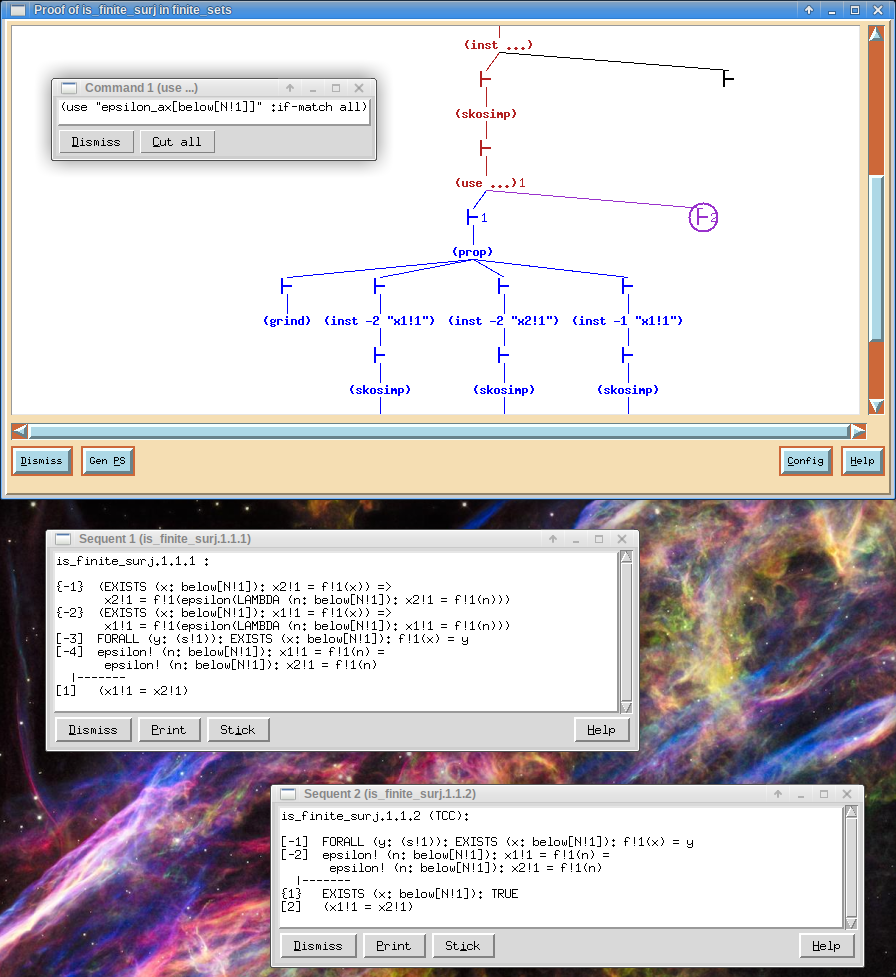
\includegraphics[width=\textwidth]{proofwindows.png}  
\caption{A Proof Display Example}\label{proofwindow}
\end{figure}

Colors are used to display status information about the proof.  These
colors may be specified using the X resource database (i.e., in your
\texttt{.Xresources} or \texttt{.Xdefaults} file).  Stipple patterns may
be specified instead of colors; a stipple pattern is specified as
\texttt{@file}, where \texttt{file} is either an absolute pathname of a
file in X bitmap format or the special bitmap name
\texttt{gray}.\footnote{If \texttt{file} is not an absolute path, it is
looked up in the \texttt{wish} subdirectory of the PVS directory, which
contains the \texttt{gray} bitmap.}

The current resources and their defaults are:

\begin{center}
\begin{tabular}{|lll|}\hline
  {\it Resource name} & {\it Color default} & {\it Monochrome default}%
     \\ \hline
  \texttt{pvs.windowbackground} & wheat & white \\
  \texttt{pvs.displaybackground} & white & white \\
  \texttt{pvs.displayforeground} & black & black \\
  \texttt{pvs.activedisplaybackground} & mediumslateblue & black \\
  \texttt{pvs.activedisplayforeground} & white & white \\
  \texttt{pvs.buttonbackground} & lightblue & white \\
  \texttt{pvs.buttonforeground} & black & black \\
  \texttt{pvs.activebuttonbackground} & steelblue & black \\
  \texttt{pvs.activebuttonforeground} & white & white \\
  \texttt{pvs.troughcolor} & sienna3 & black \\
  \texttt{pvs.currentColor} & DarkOrchid & black \\
  \texttt{pvs.circleCurrent} & yes & yes \\
  \texttt{pvs.tccColor} & green4 & black \\
  \texttt{pvs.doneColor} & blue & @gray \\
  \texttt{pvs.ancestorColor} & firebrick & black \\
  \texttt{pvs.abbrevLen} & 35 & 35 \\
  \texttt{pvs.displayfont} & \multicolumn{2}{l|}{lucidasanstypewriter-bold-12} \\
  \texttt{pvs.buttonfont} & \multicolumn{2}{l|}{lucidasanstypewriter-10} \\
  \texttt{pvs.proof.geometry} & \multicolumn{2}{l|}{\hspace*{.5in}\emph{none}} \\
  \texttt{pvs.theory-hierarchy.geometry} & \multicolumn{2}{l|}{\hspace*{.5in}\emph{none}} \\
  \texttt{pvs.prover-commands.geometry} & \multicolumn{2}{l|}{\hspace*{.5in}\emph{none}} \\
  \hline
\end{tabular}
\end{center}

The \texttt{foreground} color is used for things that aren't otherwise
specified below.  The \texttt{currentColor} is used for the current
sequent in the proof tree.  The \texttt{ancestorColor} is used for all
the ancestors of the current sequent, up to the root.  The
\texttt{doneColor} is used for sequents which have been proved.  The
\texttt{tccColor} is used for TCC's.  When \texttt{pvs.circle\-Current}
is set, the current sequent in the proof tree is circled.

Proof commands which are longer than \texttt{abbrevLen} characters are
abbreviated.

If the Emacs variable
\texttt{pvs-x-show-proofs}\index{pvs-x-show-proofs@\texttt{pvs-x-show-proofs}}
is not \texttt{NIL}, then \cmd{prove} automatically calls
\cmd{x-show-proof}.  This can be set in your
\texttt{.pvsemacs}\index{.pvsemacs@\texttt{.pvsemacs}} file.

The \cmd{x-theory-hierarchy} command prompts for a theory name and
displays the \texttt{IM\-PORTING} hierarchy rooted at that theory.  In a
complex hierarchy, it can be difficult to follow the lines; to make
this easier, when you move the mouse onto a theory identifier, all the
lines connecting that theory to other theories turn the
\texttt{highlight} color.  Clicking on a theory identifier will bring
up the theory in Emacs.  Figure~\ref{x-hierarchy} shows an example of the
theory hierarchy for the \texttt{finite\_sets} library, as produced from
clicking on the \texttt{Gen PS} button and selecting \texttt{portrait}.

\begin{figure}
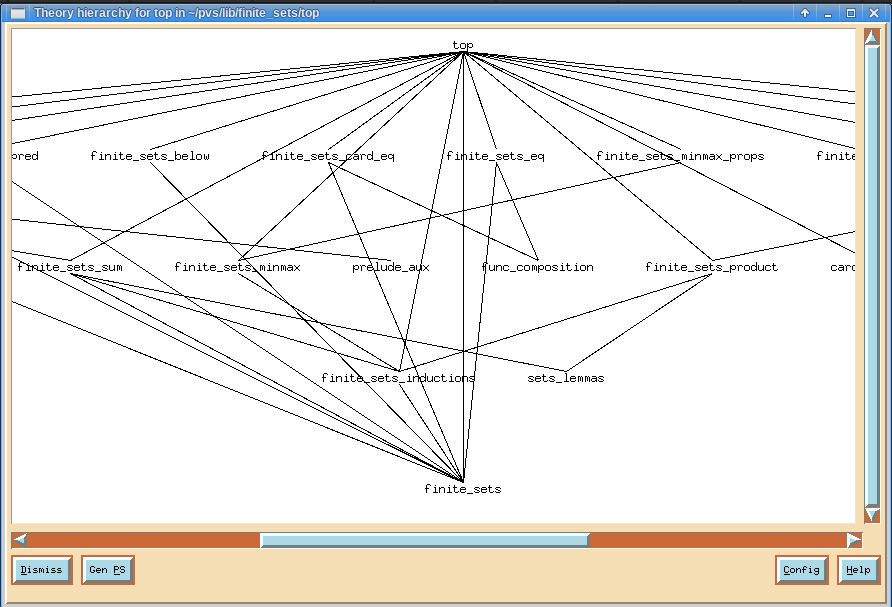
\includegraphics[width=\textwidth]{finite_sets_top_hier.png}
\caption{The Theory Hierarchy for the \texttt{finite\_sets} Library}\label{x-hierarchy}
\end{figure}


The remainder of this section applies to both \cmd{x-show-proof} and
\cmd{x-theory-hierarchy}.

The layout in the windows created by these commands can be manually
edited.  The editing commands are accessed by holding down the
\texttt{Control} key while pressing mouse buttons. In a proof window,
pressing \texttt{Control}-button~1 and dragging moves a whole proof
subtree, while \texttt{Control}-button~2 moves a single sequent.  In a
theory hierarchy window, \texttt{Control}-button~1 moves a theory.
(Note that most proof commands will do a relayout.)  Once the layout
is to your liking, the \texttt{Gen~PS} button will generate a
PostScript file which contains the contents of the window.  The
filename will be briefly displayed below the buttons.

The \texttt{Config} button will bring up a menu which will let you
customize the horizontal and vertical separations used by the
automatic layout for the current window.  These can also be customized
with the resource database.

\begin{center}
\begin{tabular}{|ll|}\hline
  {\it Resource name} & {\it Default} \\ \hline
  \texttt{pvs*proof*xSep} & 10 \\
  \texttt{pvs*proof*ySep} & 20 \\
  \texttt{pvs*th-hier*xSep} & 50 \\
  \texttt{pvs*th-hier*ySep} & 100 \\
  \hline
\end{tabular}
\end{center}


\section{Context Commands}

\begin{pvscmds}
\icmd{list-pvs-files} & \icmd{lf} & Display a list of PVS files in current context \\
\icmd{list-theories} & \icmd{lt} & Display a list of theories in current context \\
\icmd{change-context} & \icmd{cc} & Switch to a new context \\
\icmd{save-context} & \icmd{sc} & Save the current context \\
\icmd{pvs-remove-bin-files} & & Remove the \texttt{.bin} files of the current
context \\
\icmd{pvs-dont-write-bin-files} & & Inhibit writing or loading of
\texttt{.bin} files \\ 
\icmd{pvs-do-write-bin-files} & & Allows writing and loading of
\texttt{.bin} files (default) \\
\icmd{context-path} & \icmd{cp} & Display pathname of current context \\
\end{pvscmds}

The \cmd{list-pvs-files} and \cmd{list-theories} commands prompt for a
directory, default is to the current directory; if there is a PVS
context in the given directory, these commands list the PVS files or
theories in that context.  The resulting buffer is in a special mode,
which allows the file/theory to be viewed (by typing a ``\texttt{v}''),
selected (by typing a ``\texttt{s}'') or imported (by typing an ``{\tt
i}'').  A file or theory may only be selected if it is in the current
context, and may only be imported if it is not.  Importing a theory from
the list of theories will import the associated file.

The \cmd{change-context} command is similar to the ``\texttt{cd}'' command
in \unix; it saves the context (see below), and changes the working
directory to the specified one.  The \ibuf{PVS Welcome} buffer is then
displayed indicating the new directory.  If the requested directory does
not exist, and the Emacs you are running supports \texttt{make-directory},
then PVS offers to make a new one, including parent directories if necessary.
If the command fails for any reason, then the current context
stays the same.

The \cmd{save-context} command saves the current state of the session in
the context file \texttt{.pvscontext}.  In addition, any PVS files that
have been typechecked will generate a binary (\texttt{.bin}) file, unless
there is already a current one saved, or the \cmd{dont-write-bin-files}
command has been invoked.

Under normal circumstances, binary (\texttt{.bin}) files \index{.bin@\texttt{.bin}} corresponding to
the specification (\texttt{.pvs}) files are updated or created as needed.
These binary files contain type information, so that loading a binary file
has the same effect as typechecking the corresponding PVS file, but is
generally much faster.  The down side is that binary files take more disk
space.  If that is a problem then use the \cmd{pvs-dont-write-bin-files},
which neither loads nor creates binary files.  This can be added to your
\texttt{.pvsemacs}\index{.pvsemacs@\texttt{.pvsemacs}} file, by adding the
line
\begin{alltt}
  (pvs-dont-write-bin-files)
\end{alltt}
The \cmd{pvs-do-write-bin-files} undoes the effect of the
\cmd{pvs-dont-write-pvs-files}, and is not needed normally.  The
\cmd{pvs-remove-bin-files} command may be used to remove the binary files
that have been created.

The \cmd{context-path} command uses the minibuffer to display the
directory path associated with the current context.

\glossary{[directory path:] a file pathname containing sufficient
components to uniquely identify a directory}
\glossary{[context path:] a file pathname identifying the
directory which contains the context}

\section{Library Commands}

\begin{pvscmds}
\icmd{load-prelude-library} & & Extend the prelude from the specified context \\
\icmd{remove-prelude-library} & & Remove the specified context from the
prelude \\
\end{pvscmds}

The \cmd{load-prelude-library} command prompts for a context pathname
(\ie directory), and extends the prelude with all of the theories that
make up that context.  Note that the theories that make up the context are
defined by the \texttt{.pvscontext} file in the associated
directory---there may be specification files in the same directory that
are not a part of the context.  The files that make up the context are
typechecked if necessary, and internally the prelude is extended.  All of
the theories of the current context are untypechecked, as they may not
typecheck the same way in the extended prelude.  The PVS context is
updated to reflect that the prelude has been extended.  Thus the next time
this context is entered, the prelude will automatically be extended (by
typechecking the libraries if necessary).

This is just one of two means of gaining access to theories of a different
context (short of copying them).  For an alternative approach see the
language guide~\cite{PVS:language}.

The \cmd{remove-prelude-library} command removes the specified library
from the prelude.  It reverts all the theories of the current context to
untypechecked to guarantee that no theories depend on the removed library.
Note that the built-in prelude may not be removed this way.

\section{Browsing}

\begin{pvscmds}
\icmd{show-declaration} & \key{M-.} & Show declaration of symbol at cursor
\\
\icmd{goto-declaration} & \key{M-'} & Go to declaration of symbol at cursor \\
\icmd{find-declaration} & \key{M-,} & Search for declarations of given symbol \\
\icmd{whereis-declaration-used} & \key{M-;} & Search for declarations which reference identifier \\
\icmd{whereis-identifier-used} & \key{C-M-;} & Search for declarations which reference identifier \\
\icmd{list-declarations} & \key{M-:} & Produce list of declarations in import chain \\
\icmd{show-expanded-form} & \key{C-.} & Show expanded form of term
containing region\\
& & \emph{Arg:} also expand names from the prelude \\
\end{pvscmds}

These commands browse a specification consisting of several PVS files
and theories, providing information about where entities are declared
and used.  All of these commands browse the prelude as well as user
files.

The \cmd{show-declaration} command is used to determine the declaration
associated with the symbol or name at the cursor.  Positioning the cursor
on a name in the specification and typing \key{M-.} yields a pop-up
buffer displaying the declaration.  This command is useful to determine
the type of a name, or the resolution determined by the typechecker for an
overloaded name.  Note that when used on a record accessor it will
display the declaration of the record rather than just the record field.

The \cmd{goto-declaration} command goes to the declaration associated with
the symbol or name at the cursor.  It pops up a buffer containing the
theory associated with the declaration, and positions the cursor at the
declaration.

The \cmd{find-declaration} command takes a name and returns a list of all
the declarations with that name, the default name is the one under the
cursor. Each row in the display specifies the declaration name, its
kind/type, and the theory to which it belongs.  Declarations in this list
may be viewed by placing the cursor on the row of interest and typing
``\texttt{v}.''  Typing ``\texttt{s}'' will read in the associated file
and position the cursor at the declaration.  A ``\texttt{q}'' quits and
removes the declaration buffer.

The \cmd{whereis-declaration-used} command generates a list of
declarations which reference the entity denoted by a given identifier.
The related \cmd{whereis\-identifier-used} command generates a list of all
references to a \emph{textually identical} identifier, which may or may
not result from the same declaration, due to overloading and multiple
declarations.  The \cmd{list-declarations} command generates a listing of
all the declarations in the import chain of the specified theory.  For all
of these commands, the resulting buffer behaves exactly as described for
\icmd{find-declaration}.

The \cmd{show-expanded-form} command displays the expanded form of the
term containing the region in the \texttt{Expanded Form} buffer.  Each
variable, constant and operator is expanded to its full name including the
theory name and its parameters, unless they are from the current theory or
the prelude.  With an argument, prelude names are also expanded.  If the
region is not defined, the current cursor location is used instead.

%\memo{How about a \LaTeX\ version?}

\section{Theory Status}

\begin{pvscmds}
\icmd{status-theory} & \icmd{stt}, \key{C-c C-s t} & Status of specified theory (parsed, etc.) \\
\icmd{status-pvs-file} & \icmd{stf}, \key{C-c C-s f} & Status of theories of current file \\
\icmd{status-importchain} & \icmd{sti}, \key{C-c C-s i}  & Status of theories in import chain of theory \\
\icmd{status-importbychain} & \icmd{stb}, \key{C-c C-s b} & Status of
theories in import by chain \\
\end{pvscmds}

These commands provide information regarding the status of the
specified theories.  The status information for a theory indicates whether
it is parsed or typechecked, and provides the number of formulas, the
number proved, the number of TCCs generated, and the number of TCCs
proved.  Note that the number of formulas does not include the TCCs.

The number of theory warnings and messages is also displayed.  See the
\cmd{show-theory-warnings} and \cmd{show-theory-messages} on
page~\pageref{tc-info} for more information on these commands.

The \cmd{status-theory} command provides the status of the specified
theory in the mini\-buffer.  The \cmd{status-pvs-file},
\cmd{status-importchain}, and \cmd{status\-importbychain} commands display
the information in the \ibuf{PVS Status} buffer with a line for each
theory.  Using any of these commands on the \texttt{sum} theory yields
{\small
\begin{alltt}
sum is typechecked: 1 formula, 1 proved; 2 TCCs, 2 proved; 0 warnings; 0 msgs
\end{alltt}}
The \cmd{show-theory-warnings} and \cmd{show-theory-messages}
(page~\pageref{tc-info}) may be used to see any warnings or messages.

The \cmd{status-importchain} and \cmd{status-importbychain} commands
display the \texttt{IM\-PORT\-ING} chains of the specified theory, indented to
indicate the tree structure.  The \cmd{status-importchain} command works
recursively down the \texttt{IMPORTING}s, displaying the status of each
theory unless it has been displayed earlier in the buffer.  The
\cmd{status-importbychain} works in the opposite direction.


\section{Proof Status}
\label{proof-status}

\begin{pvscmds}
\icmd{status-proof} & \icmd{sp}, \key{C-c C-s p} & Status of formula at cursor \\
\icmd{status-proof-theory} & \icmd{spt} & Status of formulas in theory \\
 & & \emph{Arg:} provide timing information \\
\icmd{status-proof-pvs-file} & \icmd{spf} & Status of formulas in PVS file \\
 & & \emph{Arg:} provide timing information \\
\icmd{status-proof-importchain} & \icmd{spi} & Status of formulas on importchain \\
 & & \emph{Arg:} provide timing information \\
\icmd{status-proofchain} & \icmd{spc} & Proofchain of formula at cursor \\
\icmd{status-proofchain-theory} & \icmd{spct} & Proofchain of
specified theory \\
\icmd{status-proofchain-pvs-file} & \icmd{spcf} & Proofchain of current file \\
\icmd{status-proofchain-importchain} & \icmd{spci} & Proofchain of importchain \\
\end{pvscmds}

These commands provide the status of the proofs of the indicated formulas.
The \cmd{status-proof} command uses the minibuffer to display the proof
status of the formula at the cursor.  The status can be one of
\texttt{proved}, \texttt{untried}, \texttt{unfinished}, or
\texttt{unchecked}.  Untried means that the proof has not yet been
attempted.  Unfinished means that the proof has been attempted,
but is not complete.  Unchecked means that the proof was successful at one
point, but that some changes have been made that may invalidate the proof.

The commands \cmd{status-proof-theory}, \cmd{status-proof-pvs-file}, and
\cmd{status\-proof-importchain} use the \ibuf{PVS Status} buffer
to display the proof status for all of the formulas within the theory, PVS
file, or the import chain respectively.  With an argument, these commands
display timing information as well.

The \cmd{status-proofchain} command provides a proof chain analysis of the
formula at the cursor and displays it in the \ibuf{PVS Status} buffer.
The proof chain analysis indicates whether the formula has been proved,
and analyses the formulas used in the proof to insure that the proof is
complete; lemmas used in the proof are proved and sound, \ie\ there are no
circularities (for example, using lemma $\mathcal{A}$ to prove
$\mathcal{B}$ and vice-versa).  Because judgements are used implicitly,
they may be included in the analysis even if they are not actually used.

The commands \cmd{status-proofchain-theory},
\icmd{status-proofchain-pvs-file}, and \newline
\icmd{status-proofchain-importchain} provide the proof chain analysis for
each formula of the theory, PVS file, and import chain of the specified
theory, respectively, in the \ibuf{PVS Status} buffer.

\section{Environment Commands}

\begin{pvscmds}
\icmd{whereis-pvs} & & Display the root PVS directory \\
\icmd{pvs-version} & & Display current version of PVS and underlying \lisp \\
\icmd{pvs-mode} & & Put current buffer in PVS mode \\
\icmd{pvs-log} & & Display the \ibuf{PVS Log} buffer \\
\icmd{status-display} & & Display the \ibuf{PVS Status} buffer \\
\icmd{pvs-status} & & Find out if PVS is busy \\
\icmd{pvs} & & Start the PVS process \\
\icmd{pvs-load-patches} & & Load new PVS patches \\
\end{pvscmds}

The \cmd{whereis-pvs} command is used to determine the directory where the
PVS system resides.  This is useful for finding the example specifications
and files that are part of the PVS distribution.

The \cmd{pvs-version} command displays the current version of PVS\@.

The \cmd{pvs-mode} command puts the current buffer in PVS mode.  This
command is not normally needed; buffers with a \ibuf{.pvs}
extension and buffers created by PVS are automatically put in the
proper mode.

Most of the messages that appear in the minibuffer are kept in the
\ibuf{PVS Log} buffer, stamped with the time.  The \cmd{pvs-log} command
simply pops up the \ibuf{PVS Log} buffer so that you may view it.

The \cmd{status-display} command simply displays the \ibuf{PVS Status}
buffer.  This is the buffer used for most of the status commands.

The \cmd{pvs} command is what is used to actually start PVS after the
Emacs files have all been loaded.  It is provided as a user command
because there are times when the PVS lisp subprocess has been killed and
you wish to start up that process while keeping the same Emacs session.

The \cmd{pvs-load-patches} command reloads the patches.  This is useful
when new patches have been installed, and you wish to load them without
exiting the system and starting up again.


\section{Interrupting PVS}

\begin{pvscmds}
\icmd{pvs-status} & & Find out if Lisp is busy \\
\icmd{pvs-interrupt-subjob} & \key{C-c C-c} & Interrupt PVS (lisp)
  process \\
\icmd{reset-pvs} & \key{C-z C-g} & Abort PVS and resynchronize \\
\end{pvscmds}

Many PVS commands run in the background, allowing other editing
activities to proceed concurrently.  The effect of issuing new commands
while another command is running depends on the command: 
background commands placed on the command queue.  Other (nonbackground
commands) interrupt the currently running command, execute, and return
control to the interrupted command.  The Emacs status line indicates
the abbreviation of the command that is currently running, if any, or {\tt
ready}.  The \cmd{pvs-status} command provides information
about both the currently running command and the command queue.

To interrupt PVS for any reason, the following procedure is recommended.
First, if the keyboard is not responding, type the built-in Emacs
command \cmd{keyboard-quit} (\key{C-g}); it may need to be struck a few
times before there is any response---usually a beep and \texttt{Quit}
appears in the minibuffer.  This command interrupts Emacs, but has no
effect on any PVS commands that are still running.  After Emacs responds
go to the end of the \texttt{*pvs*} buffer, and type \key{C-c C-c}.  If
Lisp is able to respond, you should see the message
{\small\small
\begin{alltt}
Error: Received signal number 2 (Keyboard interrupt)
  [condition type: INTERRUPT-SIGNAL]

Restart actions (select using :continue):
 0: continue computation
 1: Return to Top Level (an "abort" restart)
[1c] PVS(22):
\end{alltt}}
You can then type \texttt{:continue 0} to keep going as it was never
interrupted, \texttt{(restore)} if you are in the middle of an ongoing
proof and want to continue from the state prior to the last \emph{atomic}
prover command (see the prover guide~\cite{PVS:prover}), or
\texttt{:continue 1} or \texttt{:reset} to abort to the top level.

The Lisp process may not be able to respond to the interrupt right away,
especially if it has started garbage collection.  If you really want to
interrupt it, type more \key{C-c C-c} interrupts; after about six of them
it is supposed to respond regardless.  This is not recommended in general
as it can leave the Lisp process in an unstable state.  Unfortunately, we
have seen Allegro Common Lisp get into a state where it is completely
unresponsive, even after several interrupts and waiting for hours for a
response.  This is rare, but if it happens the only recourse is to kill
the process and start up a new PVS session.  See below for how to do this
while allowing Emacs to continue.

The \cmd{reset-pvs} command aborts any ongoing activity in PVS; its
effects depend on whether it is issued from the \ibuf{*pvs*} buffer or
from some other buffer.  In the former case, \cmd{reset-pvs} simply
interrupts PVS as if you typed \key{C-c C-c}, as described above.  If
\cmd{reset-pvs} is issued somewhere other than the \ibuf{*pvs*} buffer,
you are asked whether to reset PVS in case the command was typed
accidentally; if not, the current command is aborted and the command queue
is emptied.

If you wish to kill the PVS Lisp process, while keeping your current Emacs
session, simply go to the \texttt{*pvs*} buffer and kill it
\icmd{kill-buffer} \key{C-x k}, then run \icmd{pvs} and the PVS Lisp
process will restart.  All your other Emacs buffers are unaffected by
this.

\setcounter{footnote}{0}
% Document Type: LaTeX
% Master File: user-guide.tex
\chapter{Customizing PVS}
\label{customization}
\index{customization}\index{PVS customization}

PVS is a complex system, and utilizes many subsystems, including Lisp,
Emacs, the X window system, and Tcl/Tk.  You can control aspects of these
subsystems by a combination of command-line arguments, environment
variables, and various files.  In this section we discuss some aspects of
the customization of these subsystems as they relate to PVS.

\section{Invoking PVS}\label{invoking-pvs}
\index{invoking PVS}\index{starting PVS}

PVS is invoked from a shell script named \texttt{pvs}\index{PVS shell
script} in the PVS directory---this is a text file, and may be examined or
copied and modified to suit your taste.  The script is a Bourne shell
script, and requires {\tt /bin/sh} to execute correctly.\footnote{On some
systems, \texttt{/bin/sh} is linked to the \texttt{bash} shell; this works
as well.}

PVS accepts a number of command-line arguments\index{PVS!command-line
arguments}\index{command-line arguments}, as well as using environment
variables.  The command-line arguments specific to PVS are
\begin{description}

\item[\texttt{-h | -help | --help}]\index{-help@\texttt{-help} command
line argument} - Print a brief description of the command line options and
exit.

\item[\texttt{-lisp} \emph{lispname}]\index{-lisp@\texttt{-lisp} command
line argument} - Specifies which lisp to use. The lisp image used for PVS
is then \texttt{pvs-\emph{lispname}}, which should be located in a
directory determined by the machine architecture.  See
Section~\ref{pvsimage}, page~\pageref{pvsimage} for details.

\label{dash-redhat}
\item[\texttt{-redhat}
\emph{redhat-release}]\index{-redhat@\texttt{-redhat} command line
argument} - Specifies the release of the Redhat Linux operating system you
are using (different PVS binaries are required for libc5 and glibc C
libraries).  PVS attempts to discover this for itself, but if the wrong
binary is chosen you can specify \texttt{4} or \texttt{5} using this
argument.  Note that Redhat 6 uses the glibc libraries, which corresponds
to the value \texttt{5}.

\item[\texttt{-runtime}]\index{-runtime@\texttt{-runtime} command line
argument} - This is only needed at SRI, where the development version of
the system is used by default.  With this option the runtime image is used
instead.

\item[\texttt{-emacs} \emph{emacsname}]\index{-emacs@\texttt{-emacs}
command line argument} - Specifies the Emacs to use; see below for
details.

\item[\texttt{-decision-procedures}
\emph{new}\texttt{|}\emph{old}]\index{-decision-procedures@\texttt{-decision-procedures}
command line argument} - Sets the default decision procedures to be used
in proofs.  See Section~\ref{decision-procedure-commands},
page~\pageref{decision-procedure-commands} for details.

\item[\texttt{-force-decision-procedures}
\emph{new}\texttt{|}\emph{old}]\index{-force-decision-procedures@\texttt{-force-decision-procedures}
command line argument} - Forces the chosen decision procedure to be used
regardless of the default decision procedure setting or which decision
procedures were used in developing a proof.  Note that with this option
there is no way to switch between the new and old decision procedures.

\item[\texttt{-nw}]\index{-nw@\texttt{-nw} command line argument} - Tells
Emacs not to use its special interface to X.

\item[\texttt{-batch}]\index{-batch@\texttt{-batch} command line argument}
- Run PVS in batch mode. See chapter~\ref{batchmode},
page~\pageref{batchmode} for details.

\item[\texttt{-timeout}:]\index{-timeout@\texttt{-timeout} command line
argument} In batch mode, this causes typechecking and individual proof
attempts to be interrupted after the given number of seconds.

\item[\texttt{-nobg}:]\index{-nobg@\texttt{-nobg} command line argument}
Normally PVS starts in the background (with the \& control operator).
This starts it in the foreground.

\item[\texttt{-raw}:]\index{-raw@\texttt{-raw} command line argument} This
runs PVS without Emacs.  This is only useful for front ends, which must do
the same initialization as done by the Emacs interface.

\item[\texttt{-v} \emph{number}]\index{-v@\texttt{-v} command line
argument} - Specifies verbosity level for PVS batch mode. See
Chapter~\ref{batchmode}, page~\pageref{batchmode} for details.

\label{dash-q-option}
\item[\texttt{-q}]\index{-q@\texttt{-q} command line argument} - A
standard emacs option to inhibit loading of the users {\tt .emacs} file,
but extended in PVS to inhibit loading of the users {\tt .pvsemacs}, {\tt
.pvsxemacs-options} and \texttt{.pvs.lisp} files on startup.

\item[\texttt{-patchlevel}
\emph{level}]\index{-patchlevel@\texttt{-patchlevel} command line
argument} - Specifies which patch files to load. Level \texttt{none} loads
no patch files. Level \texttt{rel} loads the file \texttt{patch2} from
your PVS directory, which usually contains the release versions of PVS
patches. Other valid levels are \texttt{test} (loads the files
\texttt{patch2} and \texttt{patch2-test}) and \texttt{exp} (loads the
files \texttt{patch2}, \texttt{patch2-test} and \texttt{patch2-exp}).
This option is mainly used for PVS development.


\end{description}
Any other command-line arguments are passed directly to the underlying
Emacs, including those for X windows---these are discussed
below.

In addition, the PVS script uses the environment
variables\index{PVS!environment variables}\index{environment variables}
\texttt{PVSLISP}\index{pvslisp@\texttt{PVSLISP}}\index{environment
variables!pvslisp@\texttt{PVSLISP}},
\texttt{PVSEMACS}\index{pvsemacs@\texttt{PVSEMACS}}\index{environment
variables!pvsemacs@\texttt{PVSEMACS}}, and
\texttt{PVSXINIT}\index{pvsxinit@\texttt{PVSXINIT}}\index{environment
variables!pvsxinit@\texttt{PVSXINIT}}, which may be set in your
\texttt{.cshrc} or \texttt{.login} file to specify the defaults you
prefer.  If both the environment variable and the corresponding
command-line argument are given, the command-line argument takes
precedence.  The \texttt{PVSXINIT} variable is described in
Section~\ref{windows}, page~\pageref{windows}.


\section{Emacs}
\index{Emacs|(}

The PVS system uses Emacs as its user interface, and provides a number of
files that extend Emacs for use with PVS.  For historical reasons, there
are currently a number of Emacs editors available.  Because we wanted PVS
to be freely available, we have chosen to concentrate on just \gnuemacs\
and XEmacs, which are also freely available.  To find out what version of
Emacs you are using, start up Emacs and type \iecmd{emacs-version}.  We
try to keep up with new releases of emacs and if necessary patch files
will be made available to support the new Emacs.

By default, the system uses \texttt{emacs}, which is assumed to be in your
path when you start up PVS.  You may specify a different Emacs as
specified above.  When you start PVS, is assumed (in order to supply X
resources in the correct format) that if the name of the emacs command
contains the character ``\texttt{x}'' then you are using XEmacs.

PVS loads your \texttt{\char'176/.emacs}\index{.emacs@\texttt{.emacs}}
file first (assuming you have not specified the {\tt -q} option as
described on page \pageref{dash-q-option}), followed by
\emph{PVSPATH}\texttt{/emacs/go-pvs.el}%
\index{go-pvs.el@\texttt{go-pvs.el}}, which determines which version of
emacs you are running and then loads the rest of the PVS emacs files,
including ILISP\index{ILISP}.  At this point you may receive an error from
PVS saying that your Emacs version is unknown.  PVS does not support Emacs
18 (or earlier), but we try to keep up with new Emacs versions as they are released.
Finally, the
\texttt{\char'176/.pvsemacs}\index{.pvsemacs@\texttt{.pvsemacs}} is
loaded.  If you are running XEmacs, the {\tt .pvsemacs} file will load
XEmacs options from the {\tt .pvsxemacs-options} file instead of the
standard {\tt .xemacs-options} file, as some are incompatible with
standard XEmacs.

In loading the files in this order, PVS functions and key
bindings will overwrite any conflicting ones defined in your
\texttt{.emacs} file.  \texttt{.pvsemacs} is the file to use to override
the key bindings and definitions given by PVS.  This approach was taken to
ensure that the behavior of PVS by default follows the user guide, but can
be readily modified to suit your taste.

One file that is worth noting is the
\emph{PVSPATH}\url{/emacs/emacs-src/pvs-abbreviations.el}%
\index{pvs-abbreviations.el@\texttt{pvs-abbreviations.el}} file, where the
abbreviations for many of the PVS commands are given.  You may define your
own abbreviations for commands you use a lot that don't currently have
abbreviations, by adding the appropriate lines in your \texttt{.pvsemacs}
file.  For example, adding
\begin{alltt}
  (pvs-abbreviate 'show-tccs 'st)
\end{alltt}
will make \ecmd{st} an abbreviation for \ecmd{show-tccs} in addition to
those already defined.  Note that you cannot redefine a name which is
already in use.

If you would like to byte-compile your Emacs customizations, create a
separate file, byte-compile it, and load it from your \texttt{.pvsemacs}.
Generally the kinds of forms provided in a \texttt{.pvsemacs} file are
simply variable settings and minor function definitions, and are not worth
byte-compiling.  It is only worthwhile if a function is being (re)defined
that will be invoked noninteractively and frequently, for example, if you
want to modify the way the process filter works.

\index{Emacs|)}


\section{The PVS Image}
\label{pvsimage}\index{PVS!lisp image|(}

PVS currently runs under Allegro Common Lisp on a number of different
platforms.  PVS is provided as a Common Lisp image, meaning that it
includes both the Lisp runtime system and the PVS programs, so you do not
need to have Allegro installed on your system.

There is usually just one PVS image available at a given site, and if the
system is properly installed, nothing further needs to be done.  If more
than one image is available, and the default one is not the desired one,
then it can be specified using either command-line arguments or
environment variables.  Invoking PVS with
{\smaller
\begin{alltt}
  pvs -lisp lucid -image pvs-lucid-sun4
\end{alltt}}
\noindent will use the \texttt{pvs-lucid-sun4} image.  Note that \texttt{-lisp
lucid} must be specified, so that the Emacs interface can be set up
properly.  For linux, also see the {\tt -redhat} option on page
\pageref{dash-redhat}.

Alternatively, the environment variables \texttt{PVSLISP} and
\texttt{PVSIMAGE} may be set to get the same effect.  Note that
command-line arguments take precedence.

After the PVS lisp image has started, it loads in the patch files as
specified by the {\tt -patchlevel} argument and then loads the file
{\tt .pvs.lisp} from your home directory.  This file can be used to
provide lisp customizations on a per user basis and for overriding
definitions in the patch file.

\index{PVS!lisp image|)}


\section{Window Systems}
\label{windows}

PVS was built primarily for the X window system\index{X windows}, though
it can be run from a terminal interface.
When run under X windows with the 
supported versions of Emacs, the resource name\index{resource
name}\index{PVS!resource name} will be set to \texttt{PVS}, and the
window\index{window name}\index{PVS!window name} and icon names\index{icon
name}\index{PVS!icon name} will be set to \texttt{PVS@}\textit{host\/},
where \textit{host\/} is the host name of the system on which PVS was
invoked.  These may be modified by adding command-line arguments or
setting the \texttt{PVSXINIT}\index{pvsxinit@\texttt{PVSXINIT}}%
\index{environment variables!pvsxinit@\texttt{PVSXINIT}} environment
variable.

You may customize the title and icon names by defining the function
\texttt{pvs-title-string} in your \texttt{.pvsemacs} file taking no
arguments and returning a string to be used as the title.  This function
is invoked at startup, and whenever the context is changed.  For example,
the following provides the name of the pvs path, the patch level
(\texttt{N} for none, \texttt{R} for released, \texttt{T} for test, and
\texttt{E} for experimental), the hostname, and the last two components of
the current context.

{\smaller
\begin{alltt}
    (defun pvs-title-string ()
      (format "%s%s%s:%s/"
          (trailing-components pvs-path 1)
        (cond ((stringp (cadddr *pvs-version-information*)) "E")
              ((stringp (caddr *pvs-version-information*)) "T")
              ((stringp (cadr *pvs-version-information*)) "R")
              (t "N"))
        (let ((host (car (string-split ?. (getenv "HOSTNAME")))))
          (format "@%s" host))
        (trailing-components *pvs-current-directory* 2)))
\end{alltt}}
\noindent For example, this might generate \url{pvs2.3N@photon:lib/finite_sets/}.

It is difficult to get a single setting for all of the Emacs versions; the
following table gives the arguments needed to set the resource, window,
and icon names for the various versions.

\begin{center}
\begin{tabular}{|l|l|l|l|} \hline
Emacs & Resource & Window & Icon \\ \hline\hline
emacs19 & \texttt{-rn} & \multicolumn{2}{|c|}{\texttt{-name}}\\ \hline
emacs19.29 (and later, & \multicolumn{3}{|c|}{\texttt{-name}}\\ 
including emacs20) & \multicolumn{3}{|c|}{ }\\ \hline
xemacs & \texttt{-name} & \texttt{-wn} & \texttt{-in} \\ \hline
\end{tabular}
\end{center}
\par\noindent Note: in emacs19, if \texttt{-rn} is not given, then
\texttt{-name} is used for the resource name as well.  Emacs19.29 and
later will give an error if the \texttt{-rn} argument is given.

The window name is the name used in the title bar of the PVS window, the
icon name is the name used in the icon, and the resource name is the name
referred to in the \texttt{.Xdefault} or \texttt{.Xresource} file that
controls the defaults for X clients.  An example entry for PVS in one of
these files might be
\begin{alltt}
!	PVS defaults
PVS.geometry: 80x63-0-0
PVS*pointerColor: Red
PVS*Font: *courier-medium-r-normal--12*
\end{alltt}
See the man pages for \texttt{X} and \texttt{emacs}, as well as the news
and info pages for the version of Emacs you are using for more details on
X resources.

The \texttt{PVSXINIT} environment variable may be set\footnote{Generally
environment variables are set in your shell startup file, \emph{e.g.},
\texttt{.profile} or \texttt{.cshrc}.} to a string
of command-line arguments that are then appended to the defaults described
above.  You can also change the default resource, window, and icon names,
simply by adding them to this variable (or by including them in the
command-line arguments).  Note that you should make certain that the
version of Emacs you are using matches the command-line arguments as shown
in the footnote.  You can tell that there is a mismatch when you start up
PVS and find buffers with names matching command-line arguments, \eg\
\texttt{-in} or \texttt{PVS@acorn}.

\setcounter{footnote}{0}
% Document Type: LaTeX
% Master File: user-guide.tex
% Use latex2e to process this file
\chapter{Running PVS in Batch Mode}
\label{batchmode}

To support validation runs, PVS supports a \emph{batch mode}, which
means that specifications and proofs being processed are not displayed.
In batch mode there is no direct interaction with PVS; it simply processes
whatever files or functions are provided and terminates after completing
the last of them.  PVS batch mode is built directly on the underlying
Emacs batch mode described in Section A.2 of the GNU Emacs
Manual~\cite{emacs20}.

If PVS is invoked in batch mode from a shell, then it may be interrupted
(using \texttt{C-c}), suspended (\texttt{C-z}), or run as a background
job.  The output may be redirected to a file or piped to another
command.\footnote{The Emacs batch option actually sends its output to
\texttt{stderr} rather than \texttt{stdout}; the \texttt{pvs} shell script
redirects this to \texttt{stdout}, as this is generally more useful and
easier to work with.}

To run PVS in batch mode, simply include the `\texttt{-batch}' option in
your call to PVS.  In addition, you should include one or more Emacs
source files and/or a Emacs or PVS function to run, using the `\texttt{-l}' or
`\texttt{-load}' option to load a file, and the `\texttt{-f}' or
`\texttt{-funcall}' option for a function.  For example:
\begin{alltt}
  pvs -batch -l test.el
  pvs -batch -f pvs-version
\end{alltt}
Note that the function option is severely limited, as it only allows a
function name.  This means that only functions that take no arguments may
be provided, for example, \texttt{pvs-version} or \texttt{whereis-pvs}.

Running PVS in batch mode does cause your \texttt{\char'176/.emacs} file
to be loaded, in contrast to running Emacs in batch mode.  If you want
to suppress the loading of your \texttt{.emacs}, include the
`\texttt{-q}' option, for example:
\begin{alltt}
  pvs -batch -q -l test.el
\end{alltt}

In batch mode PVS suppresses messages by default, though you can print
your own messages.  You can also control the amount of printout using the
verbose option, `\texttt{-v}', and providing a level number ranging from
\texttt{0} to \texttt{3}.
The following table summarizes the levels.
\begin{center}
\begin{tabular}{|l|l|}\hline
\textbf{level} & \textbf{printout} \\ \hline
0 & User-defined \texttt{pvs-message}s only \\
1 & Messages normally sent to the echo area and PVS errors\\
2 & Status buffers \\
3 & Proof replays \\ \hline
\end{tabular}
\end{center}

The \texttt{pvs-message} function is much like the Emacs \texttt{message}
function, but the message will get printed no matter what the level number
is.  If you want to print out only when the level is \texttt{1} or higher,
use \texttt{message} instead.  Both take a control string and an arbitrary
number of arguments.  An example is shown in Figure~\ref{batch-file}.

The file provided to the load option (`\texttt{-l}' or `\texttt{-load}')
is an ordinary Emacs file, and usually has an \texttt{.el} extension.
Inside this file you can invoke any PVS commands you want, though many of
them only make sense interactively.  For example, the \texttt{prove}
command expects the cursor to be positioned at a given formula, which is
difficult (though not impossible) to do in batch mode.  The various Tcl/Tk
commands available will not run at all because there is no X display
associated with PVS running in batch mode.  The most useful commands to
run in batch mode are listed in Table~\ref{batch-commands}.  In that table, a
\textit{filename} is a PVS file name without the \texttt{.pvs} extension,
a \textit{theoryname} is the name of a theory in the current context, and
a \textit{directory} is a Unix pathname.  These must all be given as
strings (enclosed in double quotes).  The \textit{length} and
\textit{depth} arguments are integers, and do not need any special
treatment.  PVS Emacs commands are given in Emacs lisp syntax; for
example,
\begin{alltt}
  (parse "foo")
  (set-print-depth 3)
  (save-context)
\end{alltt}

\begin{table}
\begin{center}
\begin{tabular}{|l|l|}\hline
\textbf{Command} & \textbf{Arguments} \\ \hline
\texttt{parse} & \textit{filename} \\
\texttt{typecheck} & \textit{filename} \\
\texttt{typecheck-importchain} & \textit{filename} \\
\texttt{typecheck-prove} & \textit{filename} \\
\texttt{typecheck-prove-importchain} & \textit{filename} \\
\texttt{prove-theory} & \textit{theoryname} \\
\texttt{prove-pvs-file} & \textit{filename} \\
\texttt{prove-importchain} & \textit{theoryname} \\
\texttt{set-print-depth} & \textit{depth} \\
\texttt{set-print-length} & \textit{length} \\
\texttt{set-rewrite-depth} & \textit{depth} \\
\texttt{set-rewrite-length} & \textit{length} \\
\texttt{alltt-theory} & \textit{theoryname} \\
\texttt{alltt-pvs-file} & \textit{filename} \\
\texttt{alltt-importchain} & \textit{theoryname} \\
\texttt{latex-theory} & \textit{theoryname} \\
\texttt{latex-pvs-file} & \textit{filename} \\
\texttt{latex-importchain} & \textit{theoryname} \\
\texttt{latex-set-linelength} & \textit{length} \\
\texttt{change-context} & \textit{directory} \\
\texttt{save-context} & \\
\texttt{pvs-remove-bin-files} & \\
\texttt{pvs-dont-write-bin-files} & \\
\texttt{pvs-do-write-bin-files} & \\
\texttt{status-theory} & \textit{theoryname} \\
\texttt{status-pvs-file} & \textit{filename} \\
\texttt{status-importchain} & \textit{theoryname} \\
\texttt{status-importbychain} & \textit{theoryname} \\
\texttt{status-proof-theory} & \textit{theoryname} \\
\texttt{status-proof-pvs-file} & \textit{filename} \\
\texttt{status-proof-importchain} & \textit{theoryname} \\
\texttt{status-proofchain-theory} & \textit{theoryname} \\
\texttt{status-proofchain-pvs-file} & \textit{filename} \\
\hline
\end{tabular}
\end{center}
\caption{Commands available for validation}\label{batch-commands}
\end{table}

An example of the contents of a batch file is shown in
Figure~\ref{batch-file}.  This file consists of three commands.  It prints
the message ``\texttt{Proving stamps2}'', changes to the
\texttt{\char'176/pvs/test} context, and then reruns all the proofs of the
specification file \texttt{stamps2.pvs}.  Note that
\texttt{current-prefix-arg} is set to \texttt{t} to ensure that the proofs
are retried.  This is equivalent to using \texttt{C-u} interactively.
\begin{figure}
\begin{center}
\fboxsep=10pt%
\begin{boxedminipage}{3.2in}
\begin{alltt}
(pvs-message "Proving stamps2")
(change-context "~/pvs/test")
(let ((current-prefix-arg t))
  (prove-pvs-file "stamps2"))
\end{alltt}
\end{boxedminipage}
\end{center}
\caption{Batch File Example}\label{batch-file}
\end{figure}
While PVS is running in batch mode, two possible kinds of error may be
encountered.  An Emacs error comes from badly formed batch files or
nonexistent functions.  These errors will cause the system to stop
immediately, and the error will be displayed if the level number is
nonzero.  A PVS error generates an error message (for a nonzero level
number) and abandons the current command, but allows the system to go on
to the next command.

If an emacs error is encountered that reports 'entering debugger' when
run with verbosity level 3, the full commands of the emacs debugger
are available\footnote{See the Emacs manual\cite{emacs20} for details.}.
A useful command to discover where your validation script encountered the error is:
\begin{alltt}
e (progn (set-buffer "*Backtrace*")(buffer-string))
\end{alltt}

Another potential pitfall is that PVS may appear to hang.  If this
happens, try running with verbosity level 3 as it is likely that PVS
is awaiting user input (usually a yes/no).  You may respond to such
prompts from the shell. 

\section{Validation Runs}

A validation run is simply a batch run in which the \texttt{pvs-validate}
macro is used in the batch file.  Given a \emph{log file} name, a
directory, and a sequence of PVS Emacs commands, \texttt{pvs-validate}
will change context to the specified directory and run the commands,
collecting the output into the log file.  It then compares the new results
to the previous ones, and reports whether there were any significant
differences.  An example of the use of \texttt{pvs-validate} is shown in
Figure~\ref{validate-file}.
\begin{figure}
\begin{center}
\fboxsep=10pt%
\begin{boxedminipage}{3.3in}
\begin{alltt}
(pvs-validate
  "stamps2.log"
  "~/pvs/test"
  (pvs-message "Proving stamps2")
  (set-rewrite-depth 0)
  (let ((current-prefix-arg t))
    (prove-pvs-file "stamps2")))
\end{alltt}
\end{boxedminipage}
\end{center}
\caption{Example Use of \texttt{pvs-validate}}\label{validate-file}
\end{figure}

Any number of \texttt{pvs-validate} forms may be used, and they may be
freely intermixed with other Emacs or PVS commands.  When the sequence of
commands associated with an invocation of \texttt{pvs-validate} is
complete, the log file is compared to the previous version, if it exists.
At this point PVS will report one of three messages:
\begin{itemize}
\item \texttt{Nothing to compare \textit{log} to} - the log file has not
been generated before this run.

\item \texttt{No significant changes in \textit{log}} - the current run
does not differ significantly from the last one.  A significant difference
is one that involves more than timing differences.  For example, the
message \texttt{proved in 27 seconds} is not significantly different from
\texttt{proved in 31 seconds}.

\item \texttt{Differences found since last run} - differences were
found.  The following line indicates the two log files that should be
compared to see where they differ.
\end{itemize}

This is normally all the output provided by PVS while processing a
\texttt{pvs-validate} macro, though you can get more information by
including the `\texttt{-v}' option as described above.

With minor exceptions, the log files contain the same information as
obtained with the `\texttt{-v 3}' option, but only for the commands of the
given \texttt{pvs-validate} macro.  In comparing log files, timings are
ignored.\footnote{In the future we may want to compare timings and report
those that are significantly different, but in order for this to work
properly we must get CPU times rather than real times, and make sure that
we are keeping track of the machine used for the previous validation run
For now we are only concerned with functional correctness.}

When a difference is reported, you can find out what the differences
actually are by starting up (an interactive) PVS, and bringing up the two
files in a split window.\footnote{In detail, start up PVS, use \texttt{C-x
C-f} to visit the first file, use \texttt{C-x 2} to split the window
vertically, and then use \texttt{C-x C-f} again to bring in the second
file.}  Then use \texttt{M-x pvs-compare-validation-windows}, which works
much like the Emacs \texttt{compare-windows} command, and will position
the cursor at the point where the two files differ.  Again, differences in
timing are ignored.  After analyzing the difference, you can move the
pointer in each buffer to the next position where they are the same, and
run \texttt{M-x pvs-compare-validation-windows} again to get to the next
difference.  In this way you can quickly analyze all the differences since
the last validation run.

The log files are maintained under RCS~\cite{RCS}, using the Emacs
\emph{Version Control} interface~\cite{emacs20}.  The first time
a validation run is made from a given directory, an RCS subdirectory is
created to keep the directory from being cluttered with RCS files.
If this is the first validation run for a given log file, then the log
file is created and registered to RCS.  In subsequent runs, the log file
is compared to the previous version, which will have a name including the
version number, for example, \texttt{stamps2.log.\char'176 1.8\char'176}.
If the comparison shows no significant differences, then the file is
subsequently deleted.

Note that the log files are all kept in the directory from which PVS was
run, and changing context will not affect that.  This makes it easy to
maintain a single directory that controls the validation for several
different contexts.

\section{Example Validation Run}
Here is an example of a validation run for a very simple specification.
\subsection{The Specification}
The specification is in the file \texttt{stamps.pvs}:
\begin{alltt}
stamps : THEORY
 BEGIN
  i, n3, n5: VAR nat
  stamps: LEMMA (FORALL i: (EXISTS n3, n5: i+8 = 3*n3 + 5*n5))
 END stamps
\end{alltt}
\subsection{The Validation File} 
The file \texttt{stamps.el} has the validation commands.  In this case we
are simply going to reprove the formulas of the specification file (there
is only one):
\begin{alltt}
(pvs-validate
 "stamps.log"
 "~/pvs-specs/validation"
 (pvs-message "Proving stamps")
 (let ((current-prefix-arg t))
   (prove-pvs-file "stamps")))
\end{alltt}
\subsection{The Validation Run}
Here is the validation run, with level number 1.  This shows the messages
that normally appear in the echo area at the bottom of the Emacs window
(these messages are sent to \texttt{stdout}):
\begin{alltt}
% ./pvs -batch -l stamps.el -v 1
Started initializing ILISP
Finished initializing pvsallegro
Loading compiled patch file /project/pvs/patch2.fasl
Context changed to ~/pvs-specs/validation/
Checking out ~/pvs-specs/validation/stamps.log...
Checking out ~/pvs-specs/validation/stamps.log...done
PVS Version 2.3 (No patches loaded)
Context changed to ~/pvs-specs/validation/
Proving stamps
Parsing stamps
stamps parsed in 0.02 seconds
Typechecking stamps
stamps typechecked in 0.02s: No TCCs generated
Rerunning proof of stamps
Using old decision procedures
Proving stamps.stamps.
Proving stamps.stamps..
Proving stamps.stamps...
Proving stamps.stamps....
Proving stamps.stamps.....
Proving stamps.stamps......
Proving stamps.stamps.......
stamps proved in 2.20 real, 0.58 cpu seconds
stamps: 1 proofs attempted, 1 proved in 2.20 real, 0.58 cpu seconds
Checking out ~/pvs-specs/validation/stamps.log.~1.3~...
Checking out ~/pvs-specs/validation/stamps.log.~1.3~...done
No significant changes in stamps.log
Checking in ~/pvs-specs/validation/stamps.log...
Checking in ~/pvs-specs/validation/stamps.log...done
\end{alltt}

\subsection{The Log File}
The resulting log file \texttt{stamps.log} is shown here.  This will
be used for comparison to in subsequent validation runs.
{\small
\begin{alltt}
PVS Version 2.3 (No patches loaded)
Context changed to ~/pvs-specs/validation/
Proving stamps
Restoring theories from stamps.bin
Restored file stamps (stamps) in 0.57 seconds
Rerunning proof of stamps
Using old decision procedures

stamps :  

  |-------
\{1\}    (FORALL i: (EXISTS n3, n5: i + 8 = 3 * n3 + 5 * n5))

Proving stamps.stamps.
Rerunning step: (INDUCT "i")
Proving stamps.stamps..
Inducting on i,
this yields  2 subgoals: 
stamps.1 :  

  |-------
\{1\}    (EXISTS (n3: nat), (n5: nat): 0 + 8 = 3 * n3 + 5 * n5)

Rerunning step: (INST + 1 1)
Instantiating the top quantifier in + with the terms: 
 1, 1,
this simplifies to: 
stamps.1 :  

  |-------
\{1\}    0 + 8 = 3 * 1 + 5 * 1

Rerunning step: (ASSERT)
Simplifying, rewriting, and recording with decision procedures,

This completes the proof of stamps.1.

stamps.2 :  

  |-------
\{1\}    (FORALL (j: nat):
         (EXISTS (n3: nat), (n5: nat): j + 8 = 3 * n3 + 5 * n5)
             IMPLIES (EXISTS (n3: nat), (n5: nat):
                         j + 1 + 8 = 3 * n3 + 5 * n5))

Rerunning step: (SKOSIMP*)
Repeatedly Skolemizing and flattening,
this simplifies to: 
stamps.2 :  

\{-1\}    j!1 + 8 = 3 * n3!1 + 5 * n5!1
  |-------
\{1\}    (EXISTS (n3: nat), (n5: nat): j!1 + 1 + 8 = 3 * n3 + 5 * n5)

Rerunning step: (CASE "n5!1 = 0")
Case splitting on 
Proving stamps.stamps...
   n5!1 = 0, 
this yields  2 subgoals: 
stamps.2.1 :  

\{-1\}    n5!1 = 0
[-2]    j!1 + 8 = 3 * n3!1 + 5 * n5!1
  |-------
[1]    (EXISTS (n3: nat), (n5: nat): j!1 + 1 + 8 = 3 * n3 + 5 * n5)

Proving stamps.stamps....
Rerunning step: (INST + "n3!1 - 3" 2)
Instantiating the top quantifier in + with the terms: 
Proving stamps.stamps.....
 n3!1 - 3, 2,
this yields  2 subgoals: 
stamps.2.1.1 :  

[-1]    n5!1 = 0
[-2]    j!1 + 8 = 3 * n3!1 + 5 * n5!1
  |-------
\{1\}    j!1 + 1 + 8 = 3 * (n3!1 - 3) + 5 * 2

Rerunning step: (ASSERT)
Simplifying, rewriting, and recording with decision procedures,

This completes the proof of stamps.2.1.1.

stamps.2.1.2 (TCC):   

[-1]    n5!1 = 0
[-2]    j!1 + 8 = 3 * n3!1 + 5 * n5!1
  |-------
\{1\}    n3!1 - 3 >= 0

Rerunning step: (ASSERT)
Simplifying, rewriting, and recording with decision procedures,

This completes the proof of stamps.2.1.2.


This completes the proof of stamps.2.1.

stamps.2.2 :  

[-1]    j!1 + 8 = 3 * n3!1 + 5 * n5!1
  |-------
\{1\}    n5!1 = 0
[2]    (EXISTS (n3: nat), (n5: nat): j!1 + 1 + 8 = 3 * n3 + 5 * n5)

Proving stamps.stamps......
Rerunning step: (INST + "n3!1 + 2" "n5!1 - 1")
Instantiating the top quantifier in + with the terms: 
Proving stamps.stamps.......
 n3!1 + 2, n5!1 - 1,
this yields  2 subgoals: 
stamps.2.2.1 :  

[-1]    j!1 + 8 = 3 * n3!1 + 5 * n5!1
  |-------
[1]    n5!1 = 0
\{2\}    j!1 + 1 + 8 = 3 * (n3!1 + 2) + 5 * (n5!1 - 1)

Rerunning step: (ASSERT)
Simplifying, rewriting, and recording with decision procedures,

This completes the proof of stamps.2.2.1.

stamps.2.2.2 (TCC):   

[-1]    j!1 + 8 = 3 * n3!1 + 5 * n5!1
  |-------
\{1\}    n5!1 - 1 >= 0
[2]    n5!1 = 0

Rerunning step: (ASSERT)
Simplifying, rewriting, and recording with decision procedures,

This completes the proof of stamps.2.2.2.


This completes the proof of stamps.2.2.


This completes the proof of stamps.2.

Q.E.D.
stamps proved in 19 seconds
stamps: 1 proofs attempted, 1 proved in 19 seconds


 Proof summary for theory stamps
    stamps..........................................proved - complete
    Theory totals: 1 formulas, 1 attempted, 1 succeeded.

Grand Totals: 1 proofs, 1 attempted, 1 succeeded.
\end{alltt}}

%\include{ug-buffers}

%\pagebreak
%\def\glossaryentry#1#2{\item#1}
%%\newcommand{\glossaryentry}[2]{foo #1}
%\chapter{Glossary}

%% NB: \input{ug.glo} will not work; the file is empty because of
%% \makeglossary by the time it gets here.  Instead, copy ug.glo to
%% ug.gls
%\begin{description}
%\input{ug.gls}
%\end{description}

\pagebreak
\appendix
%\chapter{The Grammar}\label{grammar}

The complete \pvs\ grammar is presented in this Appendix, along with a
discussion of the notation used in presenting the grammar.

The conventions used in the presentation of the syntax are as follows.
\index{syntax!conventions}

\begin{itemize}

\item Names in {\it italics\/} indicate syntactic classes and
metavariables ranging over syntactic classes.

\item The reserved words of the language are
      printed in \lit{tt font, UPPERCASE}.

\item An optional part {\it A\/} of a clause is enclosed in square brackets:
\opt{{\it A\/}}.

\item Alternatives in a syntax production are separated by a bar
(``\choice''); a list of alternatives that is embedded in the right-hand
side of a syntax production is enclosed in brackets, as in

\begin{bnf}
\production{ExportingName}
{IdOp \opt{\lit{:} \brc{TypeExpr \choice \lit{TYPE} \choice \lit{FORMULA}}}}
\end{bnf}


\item Iteration of a clause {\it B\/} one or more times is indicated by
enclosing it in brackets followed by a plus sign: \ite{{\it B\/}};
repetition zero or more times is indicated by an asterisk instead of the
plus sign: \rep{{\it B\/}}.

\item A double plus or double asterisk indicates a clause separator; for
example, \reps{{\it B\/}}{,} indicates zero or more repetitions of the
clause {\it B} separated by commas.

\item Other items printed in tt font on the right hand side of
      productions are literals.  Be careful to distinguish where BNF
symbols occur as literals, \eg\ the BNF brackets \brc{} versus the
literal brackets \lit{\{\}}.

\end{itemize}

\subsubsection*{Specification}
\par\noindent
\spvsbnf{bnf-theory}

\subsubsection*{Importings and Exportings}
\par\noindent
\spvsbnf{bnf-exporting}

\subsubsection*{Assumings}
\par\noindent
\spvsbnf{bnf-assuming}

\subsubsection*{Theory Part}
\par\noindent
\spvsbnf{bnf-theory-part}

\subsubsection*{Declarations}
\par\noindent
\spvsbnf{bnf-decls}

\subsubsection*{Type Expressions}
\par\noindent
\spvsbnf{bnf-type-expr}

\subsubsection*{Expressions}
\par\noindent
\spvsbnf{bnf-expr}

\subsubsection*{Expressions (continued)}
\par\noindent
\spvsbnf{bnf-expr-aux}

\subsubsection*{Names}
\par\noindent
\spvsbnf{bnf-names}

\subsubsection*{Identifiers}
\par\noindent
\spvsbnf{bnf-lexical}

\subsubsection*{Datatypes}
\par\noindent
\spvsbnf{bnf-adts}

%\setcounter{footnote}{0}
%\input{whats-new}
%\setcounter{footnote}{0}
% \input{ug-install}
% \pagebreak
%\setcounter{footnote}{0}
%\input{trouble}
%\pagebreak
\setcounter{footnote}{0}
% Document Type: LaTeX
% Master File: user-guide.tex
\chapter{Introduction to Emacs}
\label{emacs-intro}

The PVS system uses the GNU Emacs system as its user interface.  To make
effective use of PVS, you must become familiar with at least the basic
Emacs commands.  This section provides an introduction to Emacs that
should allow you to get started in PVS right away.  This Appendix
introduces enough of the basic ideas and commands of Emacs to use PVS, but
to become effective you really should consult the GNU Emacs
Manual~\cite{emacs20}.  It is also quite helpful to run through the online
tutorial.  To do this, start up PVS or Emacs, type \key{C-h t}, and follow
the instructions.

Emacs provides the primary interface to the PVS system.  We chose Emacs
as our interface for a number of reasons.  First, it is freely available,
and runs on a large number of different platforms.  It is also quite
popular; on Unix systems the \texttt{vi} editor is probably the only
editor that is used more than Emacs, but it is too limited to use as a
general-purpose interface.  In particular, it has no support for running
subprocesses.

Emacs is an extremely flexible editor, and includes a built in programming
language (Emacs Lisp) which makes it easy to increase its functionality.
There is a cost associated with this.  First, Emacs is rather large, and
takes longer to start up than smaller editors such as \texttt{vi}.  Emacs
is also quite complex, with a large number of commands and associated key
bindings that are not easy to learn.

Emacs is significantly different than other editors.  In most editors, you
start the editor, get a file, make some changes, save the file, and exit.
There is a tendency to think in terms of ``leaving'' the current file in
order to go to the next. To handle multiple files in a single session
usually requires extra care and some specialized commands.  For example,
\texttt{vi} can only focus on one file at a time, with one alternate.

In Emacs multiple buffers may be open at once, and as many can be made
visible as your screen allows.  Unlike other editors, buffers are not all
associated with files.  It is not unusual to have over a hundred buffers
associated with a single Emacs session.  It is also quite normal to have
the same Emacs session up for weeks at a time.\footnote{Some people have
even been known to use Emacs as their shell.}  When you are done editing
and saving a given file, you do not exit from that buffer, you simply go
on to the next one.

Unlike \texttt{vi}, there is no command mode.  By default an Emacs buffer
is in insert mode, and most keys on the keyboard simply insert themselves.
Emacs has a large number of interactive commands, any of which may be
bound to a key or key sequence.\footnote{It turns out that typing a letter
key actually invokes the command \texttt{self-insert-command}.}  Any
interactive command may be invoked by typing \texttt{M-x} followed by the
command.  Recall that \texttt{M-x} is gotten by holding down the
\texttt{Meta-} key and typing an \texttt{x}.  If you don't have a key
labeled \texttt{Meta-}, then look for and try the \texttt{Alt} or
$\Diamond$ keys.  If you really don't have a \texttt{Meta-} key, then the
\texttt{Esc} key will do, but in this case you must release the
\texttt{Esc} key before typing the \texttt{x}.

Commands may be bound to key sequences, in order to make typing easier.
For example, to page down repeatedly by typing \texttt{M-x
scroll-up} over and over would get quite tedious, so the key sequence
\texttt{C-v} was bound to this command.  This and most of the key bindings
of Emacs are not particularly mnemonic, but once learned they are
extremely effective.  With a little practice you will find that you don't
think about what key sequence is needed to get a particular effect---your
hands just do it automatically.

Each buffer in Emacs has an associated major mode, and any number of minor
modes.  The major mode indicates what kind of a buffer it is, and
generally defines the key bindings and functions associated with the
buffer.  This is usually determined from the file extension, so for
example the file \texttt{foo.pvs} is in \texttt{pvs-mode}, while a file
\texttt{foo.c} would normally be in \texttt{c-mode}.  Minor modes modify
the major mode.  Examples include \texttt{auto-fill-mode} and
\texttt{overwrite-mode}.

When you start up PVS, you will see the \texttt{PVS Welcome} buffer, which
takes up most of the window.  Toward the bottom of the window you will see
a line in inverse video; this is the mode line.  The last line of the
window is the minibuffer.  If you are running Emacs version 19 (or later) under X
windows, then you will see a menu line at the top of the window, and a
scroll bar to the right.  If you display more than one buffer in the
window, then the bottom of each buffer will have a mode line displaying
information for that buffer.  There will still be only one minibuffer,
however.\footnote{In Emacs 19 (and later versions), it is possible to have multiple windows,
called frames, associated with a single Emacs session.  In this case, each
frame by default has its own copy of the minibuffer.  See the Emacs manual
for more details.}

The mode line provides information relating to the buffer above it.  The
first five characters indicate whether the buffer is read-only, and
whether the buffer has changed relative to the file.  If you see
\texttt{---\%\%-}, then the file is read-only, and you will not be allowed
to modify it.  Sometimes this is set when you have copied a file from
somewhere else, and you think you should be able to make modifications.
In that case, use the \texttt{toggle-read-only} command, make your
changes, and save the file.  Emacs may still ask whether it should try to
save the file anyway, go ahead and answer yes in this case.

If the mode line is 5 dashes (\texttt{-----}), then the file can be
modified but has not yet been changed.  Once modified, the mode line
changes to \texttt{--**-}.  If you did not intend to modify the file, then
use the \texttt{undo} commands described below to undo your change.  If there are a
few changes, you may need to repeat the \texttt{undo} command until they
are all backed out.  If there are a lot of changes, then \texttt{M-x
revert-buffer} may be used to restore the buffer from the original file.
The other information in the mode line is the buffer name, possibly the
time, the mode of the buffer in parentheses, and the amount of the buffer
currently displayed.  Like everything else in Emacs, the mode line is
customizable; see the Emacs manual for details.

The minibuffer is used to display messages, echo longer commands as they
are typed in, and prompt for arguments.  Many of these arguments support
\emph{completion}, which means that you can type the start of an argument
and type a \texttt{TAB} to have it automatically filled in.  Emacs will
fill in as much as is unique, and then wait for more input.  If it is
ambiguous already, Emacs will pop up a buffer with the possible
completions in it.  You can force it to show all possible completions by
typing a \texttt{?}.  Not all arguments support completion, but it is
usually worthwhile to try typing a \texttt{TAB} after typing the start of
an argument to see if completion is supported; if it is then you will
either get a pop up buffer or a (partial) completion of what you typed.
Otherwise you will simply get a \texttt{TAB} inserted.

Each buffer has associated with it a current \emph{region}, which is
defined by two different locations within the buffer, called \emph{point}
and \emph{mark}.  Point is normally the cursor position, so any of the
cursor motion commands automatically move point.  Mark is not directly
displayed; it is set by command, and does not move until another mark
setting command is issued.  There are a large number of Emacs commands
that work on regions, though by far the most common usage is for cutting
and pasting operations.

%PVS uses \emacs\ as its basic interface, but does not attempt to ``take
%over'' the system---all the underlying capabilities of \emacs\ are still
%available.  Thus you can read your email, scan the news bulletins, edit
%non-PVS files, or execute commands in a shell buffer in the usual way.
%Many of the PVS commands allow you to do these while waiting for the
%command to finish.  This is especially useful for typechecking large
%specifications or while running proofs in the background.


\section{Leaving Emacs}
\begin{pvscmds}
\icmd{save-buffers-kill-emacs} & \key{C-x C-c} & Kill Emacs \\
\end{pvscmds}

This command exits Emacs, after first prompting whether to save each
modified file.


\section{Getting Help}
\begin{pvscmds}
\icmd{info} & \ikey{C-h i} & Read Emacs documentation\\
\icmd{help-with-tutorial} & \ikey{C-h t} & Display the Emacs tutorial \\
\icmd{command-apropos} & \ikey{C-h a} & Show commands matching a string \\
\icmd{describe-key} & \ikey{C-h k} & Display name and documentation a key
runs \\
\icmd{describe-function} & \ikey{C-h f} & Display documentation for
function \\
\icmd{describe-bindings} & \ikey{C-h b} & Display a table of key bindings
\\
\end{pvscmds}

These commands provide help.  When you type the \key{C-h} prefix key, you
are prompted for the next key, and can type \texttt{?} to find out all the
possibilities---only a few are described here.

The \cmd{info} command brings up a buffer containing the Emacs online
documentation.  Type \texttt{m} followed by a topic name to view the info
page for that topic, or click mouse button 2 over the highlighted name.

The \cmd{help-with-tutorial} command brings up an Emacs tutorial.  This
tutorial is interactive, inviting you to try out the commands as it
describes them.  If you are new to Emacs, you should try to go through
this at least once.

The \cmd{command-apropos} command displays a list of those commands whose
names contain a specified substring.  This is helpful if you know only
part of a command name, or suspect there is some command available for
performing some task, but do not know what it might be named.  For
example, you might do an \key{C-h a} on \texttt{mail} to find out what
mail commands are available.  If you know the beginning of a
command, it is usually better to simply start typing the command and use
the completion mechanism.

The \cmd{describe-key} and \cmd{describe-function} commands provide the
same information, but one prompts for a key and the other for a command
(with completion).  The key is not necessarily a single
keystroke, as some keystrokes are defined to be prefix keys.  In this case
the key typed so far will be displayed in the minibuffer, and the function
description will not be given until a completed key sequence has been
typed.

The \cmd{describe-bindings} command displays the key bindings in effect in
a separate buffer.  Many of these key bindings are specific to
the buffer mode, so issuing this command from different buffers will
generally lead to different results.


\section{Files}
\begin{pvscmds}
\icmd{find-file} & \key{C-x C-f} & Read a file into Emacs \\
\icmd{save-buffer} & \key{C-x C-s} & Save a file to disk \\
\end{pvscmds}

The file commands are needed to read a file into Emacs and save the
changes.  The \cmd{find-file} creates a new buffer with the same name as the
file and reads the file contents into it.  Completion is available on the
file name, including the directory.  If the file does not exist, then an
empty buffer is created.  Note that the buffer is not the same as the
file, and changes made to the buffer are not reflected in the file until
the file is saved.

The \cmd{save-buffer} command saves the current buffer to file.  If the
current buffer is not associated with a file, you are prompted to give a
file name.


\section{Buffers}
\begin{pvscmds}
\icmd{switch-to-buffer} & \key{C-x b} & Select another buffer \\
\icmd{list-buffers} & \key{C-x C-b} & List all buffers \\
\icmd{kill-buffer} & \key{C-x k} & Kill a buffer \\
\end{pvscmds}

The \texttt{switch-to-buffer} command is used to switch control from one
buffer to another.  When you type the command, you will be prompted for a
new buffer to switch to, and a default will be given.  If the default is
the right one, simply type the return key.  Otherwise type in the name of
the buffer you desire.  Completion is available.  If the buffer specified
does not already exist, then it is created.

The \texttt{kill-buffer} command is used to remove a buffer.  Completion
is available.  Note that some buffers have processes associated with them,
and killing that buffer also kills the associated process.  In particular,
the \texttt{*pvs*} buffer is associated with the PVS process.

The \texttt{list-buffers} command lists all the buffers currently
available, along with an indication of whether the buffer has changed,
its size, its major mode, and its associated file, if any.


\section{Cursor Motion commands}
\begin{pvscmds}
\icmd{forward-char} & \key{C-f} & Move forward one character \\
\icmd{backward-char} & \key{C-b} & Move backward one character \\
\icmd{forward-word} & \key{C-f} & Move forward one word \\
\icmd{backward-word} & \key{C-b} & Move backward one word \\
\icmd{next-line} & \key{C-n} & Move down one line vertically \\
\icmd{previous-line} & \key{C-p} & Move up one line vertically \\
\icmd{beginning-of-line} & \key{C-a} & Move to the beginning of the line \\
\icmd{end-of-line} & \key{C-e} & Move to the end of the line \\
\icmd{beginning-of-buffer} & \key{M-<} & Move to the beginning of the
buffer \\
\icmd{end-of-buffer} & \key{M-<} & Move to the end of the buffer \\
\end{pvscmds}

These are largely self explanatory; the best way to get used to what they
do is to simply try them out.  Note that, depending on your Emacs
environment, you may have appropriate key bindings for the arrow, Home,
PageUp, etc. keys.\footnote{As described above, you can find out what
these are bound to by typing \key{C-h k} followed by the key.}

\section{Error Recovery}
\begin{pvscmds}
\icmd{keyboard-quit} & \ikey{C-g} & Abort partially typed or executing
command \\
\icmd{undo} & \key{C-x u}, \key{C-\_} & Undo one batch of changes \\
\icmd{revert-buffer} & & Revert the buffer to the file contents \\
\icmd{recenter} & \key{C-l} & Redraw garbaged screen \\
\end{pvscmds}

\key{C-g} is used if you start to type a command and change your mind, or
a command is running and you want to abort it.  Sometimes it takes two or
three invocations before it has the desired effect.  For example if you
started an incremental search, the first \texttt{C-g} erases some of the
input and the second actually quits the incremental search.

The \cmd{undo} command is the normal way to undo changes made to the
current buffer.  If you undo twice in a row, then the last two changes are
undone.  In this manner you can eventually undo all the changes made to a
buffer.  Once you type something other than an undo, all the previous undo
commands are treated as changes that themselves can be undone.

If you made a large number of changes to a file buffer and simply want to
go back to the original file contents, use \ecmd{revert-buffer}.  Note that if you
have changed the file and saved it, then reverting will bring back the
saved version, not the earlier one.


\section{Search commands}
\begin{pvscmds}
\icmd{isearch-forward} & \key{C-s} & Incremental search forward \\
\icmd{isearch-backward} & \key{C-r} & Incremental search backward \\
\end{pvscmds}

These search through the text for a specified string.  The search is
incremental in that it starts searching as soon as a character is typed
in, finding the first occurrence of the string typed in so far.  If the
string can't be found, the minibuffer changes its prompt from
\texttt{I-search:} to \texttt{Failing I-search:}.  If it finds the string,
but you wish to go on to the next (previous) occurrence, type another
\key{C-s} (\key{C-r}).  To terminate the search, type the Enter key, or
any other Emacs command.  Consult the Emacs manual for other useful
options available for search.


\section{Killing and Deleting}
\begin{pvscmds}
\icmd{delete-next-character} & \key{C-d} & Delete next character \\
\icmd{delete-backward-char} & \key{DEL} & Delete previous character \\
\icmd{kill-word} & \key{M-d} & Kill word \\
\icmd{backward-kill-word} & \key{M-DEL} & Kill word backwards \\
\icmd{kill-line} & \key{C-k} & Kill rest of line \\
\icmd{kill-region} & \key{C-w} & Kill region \\
\icmd{copy-region-as-kill} & \ikey{M-w} & Save region a killed text
without killing \\
\end{pvscmds}

These commands delete or kill the specified entities.  The difference
between killing and deleting is that a killed entity is copied to the kill
ring, and can be \emph{yanked} later, while deleted entities are not.  The
kill ring is a stack of blocks of text that have been killed, with the
most recent kills at the top.  The kill ring is not associated with any
specific buffer, and in this respect acts much like a \emph{clipboard}
found in most window systems.

The \cmd{delete-backward-char} command is frequently mapped onto the
\ikey{Backspace} key instead; you may need to experiment with this. If
you want it mapped to the \key{Backspace} key, it is usually easier to map
it outside of Emacs, for example using the \texttt{xmodmap} command.  This
is because by default the \key{Backspace} key and the \key{C-h} key are
indistinguishable by Emacs, and the \key{C-h} key is used for accessing
various Emacs help functions.

The \cmd{kill-line} command kills from the current cursor location to the
end of the line, unless it is already at the end of the line, in which
case it kills the newline, thus merging the current line with the
following one.

The \cmd{copy-region-as-kill} command is similar to the \cmd{kill-region}
command, but does not actually kill any text.  This is useful when trying
to copy text from a file for which you do not have write access, since
Emacs will not let you modify such a buffer without first changing its
read-only status.

\section{Yanking}
\begin{pvscmds}
\icmd{yank} & \ikey{C-y} & Yank last killed test \\
\icmd{yank-pop} & \ikey{M-y} & Replace last yank with previous kill \\
\end{pvscmds}

The \cmd{yank} command puts the text of the most recent kill command into
the buffer at the current cursor position.  Note that the usual way to
move text from one place to another in Emacs is to kill it, move the
cursor to the new location, and yank it.  Because the kill ring is
globally used, this works across buffers as well.

The \cmd{yank-pop} command may only be used after the \cmd{yank} command,
and has the effect of replacing the yanked text with earlier killed text
from the kill ring.

\section{Marking}
\begin{pvscmds}
\icmd{set-mark-command} & \ikey{C-\char064}, \ikey{C-SPC} & Set mark here \\
\icmd{exchange-point-and-mark} & \ikey{C-x C-x} & Exchange point and mark
\\
\end{pvscmds}

The \cmd{set-mark} command sets the mark to the current cursor position.
Since point is also at the current cursor position, this defines an empty
region initially.  As the cursor is moved away from the mark position, the
region grows.  Note that the relative positions of mark and point do not
matter; the region is defined as the text between these two positions.

\key{C-x C-x} is used to exchange the point and mark positions, moving the
cursor to where mark was last set, and setting mark to the old cursor
position.  Doing this again puts mark and point back where they started.
This is useful for checking that the region is as desired, before doing
any destructive operations.
 
\pagebreak
\setcounter{footnote}{0}
%{\small
%% Document Type: LaTeX
% Master File: user-guide.tex
\chapter{Errors}
\label{errors}
\index{errors}

This Appendix lists all the possible \pvs\ errors, along with a brief
explanation of their cause and possible solutions.  The errors are split
into \emacs\ errors, parser errors and typechecker errors.  For a
discussion of possible prover errors, see the PVS prover manual.

%\section{\emacs\ Errors}

\memo{Need to systematically check through the source code for
any new error messages, and to remember to update this document if
any new error messages are added in the future.}

\memo{Should the error messages occur in the index?}

\section{Parser Errors}

\begin{description}

\item[There is garbage at the end of your file or string:] - the parser
has parsed the file or string, and found more tokens after scanning a
complete nonterminal.

\item[End id {\em foo\/} does not match theory id {\em bar\/}] - indicates
that the identifier at the end of the theory is different from the
identifier at the beginning.

\item[End id {\em foo\/} does not match datatype id {\em bar\/}] -
indicates that the identifier at the end of the datatype is different from
the identifier at the beginning.

\item[Found \emph{foo} when expecting \emph{bar},\ldots] - this error
indicates that the wrong kind of token was found here, and gives a
somewhat arcane indication of what was expected.  If the error isn't
obvious, look at the grammar in the language manual, and keep in mind that
the position of the cursor may be beyond the actual cause of the error.

\item[\emph{foo} expected here] - this error is usually easy to diagnose
and fix, since the message indicates what is expected at the cursor
location.

\item[Inline datatypes may not have parameters] - this error indicates
that the parameters were provided to an inline datatype.  Note that if an
attempt is made to provide parameters in square brackets, an ``End
expected here'' error will result.

\item[Only one id allowed for datatypes] - it is illegal (and usually
undesirable) to give multiple datatypes in a single declaration.  If you
really want to do this, simply split the datatype apart---making one copy
for each identifier.

\item[Datatype identifier must be an id] - you may not use an operator
such as \texttt{+} as a datatype identifier.  It must be a letter followed
by any number of letters, digits, underscores, and question marks.

\item[May not have multiple ids with `\texttt{|}'] - expressions such as
\texttt{FORALL (x,y,z|p):\ foo} are illegal, and should either be written
as \texttt{FORALL x,y,(z|p):\ foo} or \texttt{FORALL x,y,z:\ p IMPLIES foo}.

\item[Enumeration types are only allowed at the top level] - this is
because enumeration types are translated into inline datatypes, which
generate a number of new top-level declarations.

\item[Function type must have a range] - the \texttt{FUNCTION} keyword was
used, but a range type (preceded by an arrow (\texttt{->}) was not given.

\item[Illegal character name] - this is an illegal name for a character.
The legal names are displayed in the table below.
\def\ct{\symbol{'136}}
\texttt{\begin{center}
\begin{tabular}{|cccccccc|}\hline
\ct @ & \ct A & \ct B & \ct C & \ct D & \ct E & \ct F & \ct G \\
\ct H & \ct I & \ct J & \ct K & \ct L & \ct M & \ct N & \ct O \\
\ct P & \ct Q & \ct R & \ct S & \ct T & \ct U & \ct V & \ct W \\
\ct X & \ct Y & \ct Z & \ct [ & \ct\symbol{'134} & \ct ] & \ct\ct & \ct\symbol{'137} \\
SP & ! & " & \# & \$ & \% & \& & ' \\
( & ) & * & + & , & - & . & / \\
@ & A & B & C & D & E & F & G \\
H & I & J & K & L & M & N & O \\
P & Q & R & S & T & U & V & W \\
X & Y & Z & [ & \symbol{'134} & ] & \ct & \symbol{'137} \\
` & a & b & c & d & e & f & g \\
h & i & j & k & l & m & n & o \\
p & q & r & s & t & u & v & w \\
x & y & z & \{ & | & \} & \symbol{'176} & \ct? \\ \hline
\end{tabular}\end{center}}

\item[Projection may not have actuals] - you may not include actuals with
a projection name, since projections do not belong to any theories.

\item[Projection may not have a theory id] - you may not include a theory
id with a projection name, since projections do not belong to any
theories.

\item[Projection may not have a library id] - you may not include a
library id with a projection name, since projections do not belong to any
libraries.

\item[Invalid id] - PVS identifiers must start with a letter, followed by
any number of letters, digits, underscores, or question marks.

\end{description}


\section{Typechecker Errors}

The typechecker errors are presented in subsections mostly based on
language constructs.

\subsection{Importing Errors}

\begin{description}

\item[Can't find file for theory \emph{foo}] - this error indicates that
there is an exporting of a theory that is not known in the context and a
file with the same name as the theory could not be found.  You must find
or create the specified theory and typecheck it before typechecking the
current theory.

\item[Wrong number of parameters] - a theory name was given with the wrong
number of actual parameters.  Compare the formal parameters of the theory
with the actual parameters given in the theory name; make sure that you
are not counting the \texttt{IMPORTING}s in the formal parameters.

\item[Theory {\em foo} is not in the IMPORTINGs] - this error results from
the use of a name of the form \texttt{\emph{foo}.\emph{bar}}, and the
theory \emph{foo} is neither a part of the prelude, nor has it been
previously imported to the theory.

\item[A theory may not import itself] - the current theory appears on an
importing chain.

\item[Theory {\em foo\/} not found] - this error occurs during the
typechecking of an importing clause, and indicates that the theory
\emph{foo} was not found in the current context.

\item[Wrong number of parameters] - in an importing clause, the indicated
theory has the wrong number of actual parameters given.

\item[Circularity found in importings of theories] - this error indicates
that there is a circularity in the closure of the importings clauses.  The
cursor is placed at the beginning of one of the offending theories, and a
list of theory names involved in the circularity is displayed.

\end{description}


\subsection{Exporting Errors}

\begin{description}

\item[May not export formal parameters] - an attempt was made to export a
formal parameter.  This is not allowed, as formal parameters are not
visible from outside the module.

\item[Name {\em foo\/} is not declared in this theory] - an attempt was
made to export an entity that was not declared in the current module.  For
further details on the use and restrictions of the exporting clause, see
the language manual.

\item[Name {\em foo\/} is not declared as {\em kind\/} in this theory] -
when names are overloaded, a kind (or type) may be included in the
exporting clause to specify which entity is actually exported.  This error
indicates that there is no entity of the kind (or type) specified.

\item[{\em foo\/} may not be exported] - this error indicates that an
attempt was made to export a variable or a field declaration.  Variable
declarations may not be exported, and field declarations are automatically
exported when the associated record type is, and may not be exported
otherwise.

\item[{\em foo\/} may not be exported unless the following are also: {\em
bar$_1$\/},\ldots] - entities may only be exported if all of the
declarations on which they depend are also exported.

\item[{\em foo\/} refers to {\em name\/}, which must be exported] -
entities may only be exported if all of the declarations on which they
depend are also exported.

\item[{\em foo\/} occurs in an EXPORTING WITH but is not in an IMPORTING
clause] - only theories that are imported may be exported.

\end{description}


\subsection{Declaration Errors}

\begin{description}

\item[Coercion must be a constant] - this error is associated with
coercion declarations, which only apply to constants, recursive
definitions, and inductive definitions.

\item[Coercion is not a unary function: \emph{foo}] - this error is given
when the constant to be used as a coercion has a domain with more than one
component.

\item[The domain and range of this coercion are compatible; the coercion
will never] \textbf{be used: \emph{foo}} - because coercions only take place when
there is otherwise a type error, if the domain and range are compatible
then the coercion would never be automatically applied.  Strictly
speaking, this does not have to be an error, but it is treated as such
because it is clearly not what is intended.  See the language manual for
more discussion.

\item[May not overload projection names] - an attempt has been made to
redeclare a projections name of the form \texttt{PROJ\_}$n$ (or some
variant of this with different cases, such as \texttt{Proj\_}$n$).  Because
of the special status of these names,\footnote{Projections are one of the
few entities of PVS that may not be declared in PVS, even using
parameterized theories} they may not be redeclared.

\item[{\em foo\/} is the name of a formal parameter and may not be
redeclared] - within a theory a formal parameter name may not be reused.
If you really want ot use the name, change the formal parameter name since
it will not be used outside the theory anyway.

\item[{\em foo\/} has previously been declared with type {\em type\/}] -
this error indicates that an entity has already been declared in this
theory.

\item[{\em foo\/} has previously been declared with type {\em type\/},
which may lead to ambiguity] - this error indicates that an entity has
been declared with a compatible type, which may lead to ambiguity.  The
difficulty here is that in disambiguating names, after the theory, actual
parameters, and library have all been pinned down, the type should
uniquely determine the resolution of a reference, and compatible types may
not allow the typechecker to make the distinction.

\item[Name {\em foo\/} already in use as a {\em kind\/}] - this error
applies to non-expression declarations such as formulas, theory
declarations, etc.  It indicates that the same name is being used twice
for the same kind of declaration in the same theory.

\end{description}

\subsubsection{Recursive Function Errors}

\begin{description}

\item[Recursive definition must be a function type] - the type of a
recursive declaration must be a function type, or a subtype of a function
type.

\item[Termination TCC could not be generated] - This error results from a
recursive call for which arguments have not been provided.

\item[Measure must be a function] - the provided measure must resolve to a
function.

\item[Wrong number of arguments in measure] - the argument pattern of the
measure function must match that of the recursive function being declared.

\item[Measure must have range a naturalnumber or an ordinal] - the range
type of the measure function usually is a natural number, but ordinal
numbers are also supported.  No other range types are allowed.

\item[Incompatible domain types] - the domain type of the measure is
incompatible with the corresponding domain type of the recursive function
being declared.

\end{description}


\subsubsection{Inductive Declaration Errors}

\begin{description}

\item[Inductive definition must be a function type] - the type of a
inductive declaration must be a function type, or a subtype of a function
type.

\item[Inductive definitions must have (eventual) range type boolean] - see
the language manual for a discussion of this restriction.

\item[Cannot determine parity of this occurrence of the inductive
definition] - the recursive occurrences of the inductive definition must
be positive; the system could not determine the parity of this occurrence.

\item[Negative occurrences of the inductive definition are not allowed] -
the recursive occurrences of the inductive definition must be positive,
this occurrence is negative.

\end{description}


\subsection{Type Expression Errors}

\begin{description}

\item[Enumtype must be declared at top level] - since enumeration types
are really just inline datatypes, they must be declared at the top level.

\item[No type found] - this error is displayed when a parenthesized
expression is used as a type and no type for the expression is found.

\item[Does not resolve to a predicate] - this error occurs when a
parenthesized expression is used as a type and the expression does not
resolve to a predicate, \ie, a function with boolean range type.

\item[Uninterpreted subtypes are only allowed at the top level] -
\memo{Can this error be reached?}

\item[Wrong number of variables] - this error comes from typechecking a
subtype expression of the form \texttt{\{x1,\ldots,xn:T | p\}}, where
\texttt{T} is a tuple type with number of component types different from
\texttt{n}.

\item[Duplicate field names not allowed] - the same field name was used
twice in the same record type.

\end{description}


\subsubsection{Judgement Declaration Errors}

\begin{description}

\item[No declaration of specified type could be found] - this error occurs
when typechecking a judgement declaration, and indicates that the entity
being declared as a judgement could not be found matching the specified
type.

\item[Only constant names or numbers may have HAS\_TYPE judgements] -
indicates that an expression other than a name or number was provided
here.

\end{description}


\subsubsection{Type Application Errors}

\begin{description}

\item[Uninterpreted types may not have parameters] - although type
declarations may now have parameters, they are not allowed for
uninterpreted type declarations.  See the language manual for a discussion
of this restriction.

\item[Type applications may not be curried] - the parameters to a type
declaration may not be curried, \eg\
\begin{alltt}
  t(x:int)(y:int): TYPE = {z:int | z < x + y}
\end{alltt}
is not allowed, for the simple reason that partial type applications are
not allowed.

\item[\emph{foo} may not be used in a type application] - only type names
declared to be applications (\ie, with declaration parameters) may be used
in type applications.

\item[Wrong number of parameters] - a type application was given with the
wrong number of parameters.

\end{description}


\subsection{Expression Errors}

\begin{description}

\item[Wrong arity] - this error occurs with tuple expressions, and
indicates that a different number of subexpressions was expected.

\item[{\em foo\/} expected here] - this error occurs when a lambda
expression is provided where a (non-functional) type \emph{foo} is
expected.

\item[Wrong number of bound variables - $n$ expected] - the given lambda
expression has a different number of bound variables than expected.

\item[Wrong number of assignments] - the given record expression has a
different number of assignments than expected.  Recall that each field of
a record expression must be given exactly once.

\item[No compatible types] - this error occurs for an update expression
when a function type is expected and the possible types of the update
expression are not compatible with the expected type.

\item[{\em foo\/} is not a record, function, or array type] - update
expressions are only allowed for these types.

\item[Field not found] - an assignment made in a record update references
a field that was not found in the expected type.

\item[TCC for this expression simplifies to false: \emph{foo}] - the
typechecker has generated a \tcc\ and found that it reduced to
\texttt{false} when it was simplified.  This is a type error, though the
expression \emph{foo} may need careful scrutiny to determine the cause of
the error.

\item[Recursive definition occurrence {\em foo\/} must have arguments] -
the termination of a recursive function is requires every recursive call
to have at least as many arguments as the function given in the measure.

\item[Formals are not allowed in {\em foo\/}s] - this error occurs when
formal declaration arguments are provided where they are not allowed, \eg\
in \texttt{foo(x:int): FORMULA x = y} it makes no sense to provide a
formal argument, as there is no way to reference the formula name with a
parameter.  Formal declaration arguments are only allowed for type,
constant, recursive, and inductive declarations.

\item[Library \emph{foo} does not exist, or has no .pvscontext file] -
this error indicates either that a specified library pathname could not be
found, or that its directory does not contain a .pvscontext file.  Either
modify the pathname, or create the library directory and files (you will
need to use the \unix\ \texttt{mkdir} command to create the directory,
and the \iecmd{change-context} command to move to that directory and
create the files).

\item[The argument to \texttt{PROJ\_}$n$ must be a tuple with length at
least $n$] - this error is displayed when a projection function is applied
to an expression that is ``too short,'' in that the type of the expression
is a tuple with fewer than $n$ components.

\item[There must be at least $n$ arguments for \texttt{PROJ\_}$n$] - this
error occurs with expressions such as \texttt{PROJ\_3(1,2)}.

\item[Record expression assignments must not have arguments] - the
left-hand side of an assignment in a record expression may not have
arguments, \eg\ the second assignment in the expression \texttt{(\# a := 2,
(b)(3) := 1 \#)} is illegal.

\item[Record expressions must have named fields] - the left-hand side of
an assignment in a record expression must be a simple identifier.

\item[Duplicate field assignments are not allowed] - the left-hand sides
of the assignments of a record expression must all be unique simple
identifiers.

\item[Expression type must be a datatype] - in a CASES expression of the
form \texttt{CASES \emph{foo} OF \ldots}, the type of \emph{foo} must be a
datatype.

\item[Selections must have a unique id] - the indicated selection of the
CASES expression was seen earlier.

\item[ELSE part will never be evaluated] - the ELSE part of the CASES
expression was provided, but it will never be evaluated since the
selections cover all possibilities.

\item[No matching constructor found] - the datatype constructor associated
with the specified selection of the CASES expression could not be found.

\item[Wrong number of arguments] - the constructor associated with the
given selection of the CASES expression has a different number of
arguments than the selection.

\item[Incompatible types in application] - this error indicates that no
type could be found that is consistent with the operator and the
arguments.  This error should rarely occur; more specific errors will
usually be given.

\item[Type mismatch in coercion \emph{foo} Possible expression types:
\emph{type}, \ldots] - this error indicates that the type given in the
coercion expression does not match the type found for the expression.  A
simple example of this is \texttt{3:bool}.

\item[Type mismatch in application \emph{foo} Operator types:
\emph{type},\ldots Arguments types:] \textbf{\emph{type},\ldots} - This indicates
that the type of the operator and the arguments are incompatible.

\item[Must resolve to a record, function, or array] - the specified
expression of the update expression could not be resolved to one of these
types.

\item[Duplicate assignments not allowed in recordtypes] - an update on an
expression whose type is a record type was found to have two assignments
with the same left-hand sides.

\item[Field name expected] - the left-hand side of an assignment of an
update expression whose type is a record type must be a field name of that
record type.

\item[May not have partial updates for dependent record types] - a partial
update is one of the form \texttt{r WITH [(a)(b) := x]}, \ie\ an update of
a functional at a specific point.  This is not allowed for dependent
record types, mostly due to the fact that the resulting forms (\eg\
\tccs)are very difficult to understand.

\item[Wrong number of assignment arguments, $n$ expected] - in an update
assignment such as the one in \texttt{f WITH [(a$_1$,\ldots,a$_n$) := y]},
the size of the domain of the type of {\tt f} was different from $n$.
This can also happen recursively, \eg\ the following is an error:
{\small
\begin{alltt}
  (LAMBDA (x:int): (LAMBDA (y,z:int): x + y * z)) WITH [(0)(1,2,3) := 0]
\end{alltt}}

\item[The expression type is inconsistent with this set of arguments] -
this error occurs in an update expression when there are more arguments in
the left-hand side of an assignment than are allowed by the type of the
expression being updated.  An example is
{\small
\begin{alltt}
  (LAMBDA (x:int): x + 1) WITH [(0)(1,2,3) := 0]
\end{alltt}}

\item[Variable \emph{foo} not previously declared] - this error indicates
that a binding was given without a type and there was no earlier variable
declaration with that name.  For example, \texttt{(FORALL x: p(x))}, where
\texttt{x} is not previously declared as a variable (in the current
theory).

\item[Variable \emph{foo} is ambiguous] - the type of the specified
variable was not given, and there is more than one variable declaration
with the same name.

\item[{\em foo\/} does not have a unique type - one of: {\em
type$_1$\/},\ldots] - this error pertains to expressions that are not
names that are still ambiguous.  The simplest way to disambiguate these
expressions is to add a colon followed by the type.  Parentheses may be
necessary as the colon binds tightly (\eg\ \texttt{x - 1:nat} is parsed as
\texttt{x - (1:nat)}).

\item[Incompatible types Found: {\em ftype$_1$},\ldots Expected: {\em
etype\/}] - this message is displayed when there is a type mismatch.  The
types are displayed in an expanded form, so that differences may be found.
However, they are not fully expanded, as this can lead to extremely large
displays and the information is just as useless as if it was unexpanded.
If the types look identical, then you will need to do a careful analysis
of the types of the entities involved to figure out where the discrepancy
lies.  In practice, this is rarely a problem.

\item[Bound variable outside of context] - \memo{Should this still be
possible?}

\end{description}


\subsection{Name Resolution Errors}

\begin{description}

\item[{\em foo\/} does not uniquely resolve - one of: {\em
fullname$_1$},\ldots] - this error indicates that there is an ambiguity in
the use of a name.  A name may be made unambiguous by adding one or more
of the following.
\begin{itemize}
\item theory identifier
\item actual parameters
\item type
\item library identifier
\end{itemize}
The complete name of an entity is of the form
\texttt{\emph{lib}@\emph{th}[\emph{act},\ldots].\emph{id}:\emph{type}}.
See the language manual for more information.

\item[Ambiguous theory instance, could be one of:
\emph{theoryname},\ldots] - the name expression is ambiguous in that
multiple instances are available, and the typechecker is not able to
decide between them.  This usually happens when multiple instances of the
same theory are imported, and the actual parameters were left off of a
name reference.  To continue, simply supply the correct actual parameters.

\item[Could not determine the full theory instance] - this error indicates
that the typechecker was only partially able to resolve the actual parameters
of the specified name.  This frequently happens when a theory is imported
generically, and some of the parameters (usually the type parameters)
could be uniquely determined, while others could not.  To continue, simply
supply the correct actual parameters.

\item[Expression provided where a type is expected] - this error indicates
that an actual parameter is an expression, but the corresponding formal
parameter expects a type expression.

\end{description}


\subsection{Datatype Errors}

\begin{description}

\item[Duplicate enumeration names are not allowed] - the names used in an
enumeration type declaration must all be unique.

\item[Duplicate constructor names are not allowed] - the constructor names
of a datatype must all be unique.

\item[Duplicate recognizer names are not allowed] - the recognizer names
of a datatype must all be unique.

\item[{\em foo} is used as both a constructor and recognizer name] - the
constructor names must be disjoint from the recognizer names.

\item[Datatype name may not be used as a constructor name] - the
identifier used for the datatype cannot be used as a constructor.

\item[Datatype name may not be used as a recognizer name] - the
identifier used for the datatype cannot be used as a recognizer.

\item[May not have duplicate accessor names for a single constructor] -
within a single constructor form, the accessor names must be unique.

\item[Datatype name may not be used as an accessor name] - the
identifier used for the datatype cannot be used as an accessor.

\item[There must be at least one non-recursive constructor] - at least one
of the constructor forms must have no reference to the datatype itself;
see the language manual for more discussion.

\item[Recursive uses of the datatype {\em foo\/} must be (a subtype of)
one of the forms] \textbf{\emph{foo}, sequence[\emph{foo}], or a
(positive) parameter to another datatype} - see the language manual for a
full discussion of this restriction.

\item[Assumings are not allowed for in-line datatypes] - since formal
parameters are not allowed for in-line datatypes, it makes no sense to
have an assuming section.

\end{description}


\subsection{Modify Declaration Errors}
\index{modify-declaration@\texttt{modify-declaration}!errors}

These errors arise during the use of the \ecmd{modify-declaration}
command, which has many restrictions on its use.  One way around many of
these restrictions is to use \iecmd{add-declaration} instead, and to
delete the declaration that you wanted to modify later (after finishing
with any proof in progress).

\begin{description}

\item[Modified declaration must have the same type - \emph{foo}] - the
type of the declaration edited using the \ecmd{modify-declaration}
command must not be changed.

\item[Only one declaration is allowed] - you may not add new declarations
using the \ecmd{modify-declaration} command.  Use \ecmd{add-declaration}
instead, after modifying the given declaration.

\item[Modified declaration must keep the same id - \emph{foo}] - an
attempt has been made to change the identifier associated with the
declaration being modified.  Change it back to what it was and try again.

\item[Modified declaration must be the same kind - \emph{foo}] - you may
not change the class of a declaration being modified, \eg\ from a formula
to a variable.  Change it back and try again.

\end{description}

\section{\LaTeX\ Errors}

There are two kinds of \LaTeX\ errors, those that arise in reading the
\LaTeX\ substitution files (\texttt{pvs-tex.sub}), and those that are
generated as a result of executing \LaTeX.  We will not go into the latter
here, see the \LaTeX\ manual~\cite{latex2e} for help in understanding these
errors.  \memo{Describe the presentation of the errors}

The substitution errors are described below, see
section~\ref{latex-output}, page~\pageref{latex-output} for a full
definition of the terms used.

\begin{description}

\item[Incomplete substitution defined for \emph{foo}] - indicates that the
entry for \emph{foo} is incomplete; there should be four separate fields.

\item[Illegal length \emph{arg} for \emph{foo}] - indicates that the width
field was illegal for the entry for \emph{foo}; it must either be a
positive integer or a hyphen.

\item[Illegal kind or arity \emph{foo} for \emph{id}: must be KEY, ID,
number, or list of numbers] - the kind field was not one of the legal
values.

\end{description}

%}
%\input{commands}

\pagebreak
%\addcontentsline{toc}{chapter}{References}
\bibliographystyle{plain}
\bibliography{../pvs}

%\addcontentsline{toc}{chapter}{Index}   %% Put entry in T-O-C
%\printindex  %% printindex makes extra call to "theindex"
{\smaller\smaller
\printindex
%% Document Type: LaTeX
% Master File: user-guide.tex
\documentclass[12pt]{book}

\usepackage{alltt}
\usepackage{makeidx}
%\usepackage{showidx}	% use for index debugging
\usepackage{relsize}
\usepackage{boxedminipage}
\usepackage{fancyheadings}
\usepackage{graphicx}
\usepackage{../../pvs}
\usepackage{url}
\usepackage{latexsym}
\usepackage[chapter]{tocbibind}
\makeatletter
\@ifundefined{pdfoutput}%
{\usepackage[dvips=true,bookmarks=true,hyperindex=true]{hyperref}}%
{\usepackage[pdftex,dvipsnames,usenames]{color}%
\usepackage[bookmarks=true,hyperindex=true,colorlinks=true,linkcolor=Brown,citecolor=blue,backref=page,pagebackref=true,plainpages=false,pdfpagelabels]{hyperref}%
}%
\makeatother

\topmargin -10pt
\textheight 8.5in
\textwidth 6.0in
\headheight 15 pt
\columnwidth \textwidth
\oddsidemargin 0.5in
\evensidemargin 0.5in   % fool system for page 0
\setcounter{topnumber}{9}
\renewcommand{\topfraction}{.99}
\setcounter{bottomnumber}{9}
\renewcommand{\bottomfraction}{.99}
\setcounter{totalnumber}{10}
\renewcommand{\textfraction}{0}
\renewcommand{\floatpagefraction}{.01}

\raggedbottom

%\input{/project/pvs/doc/prelude}
\def\labelitemii{$\circ$}
\def\labelitemiii{$\star$}
\def\labelitemiv{$\diamond$}
\newcommand{\tcc}{{\small\small TCC}}
\newcommand{\tccs}{\tcc s}

%\renewcommand{\memo}[1]{\mbox{}\par\vspace{0.25in}\noindent\fbox{\parbox{.95\linewidth}{{\bf Memo: }#1}}\vspace{0.25in}}

\newcommand{\eg}{{\em e.g.\/},}
\newcommand{\ie}{{\em i.e.\/},}

\newcommand{\pvs}{PVS}

\newcommand{\ch}{\choice}
\newcommand{\rsv}[1]{{\rm\tt #1}}

\newcommand{\lpvstheory}[3]{\figurehead{\hozline\smaller\smaller\begin{alltt}}%
                           \figuretail{\end{alltt}\vspace{-0in}\hozline}%
                           \figurelabel{#3}\figurecap{#2}%
                           \begin{longfigure}\input{#1}\end{longfigure}}

\newcommand{\bpvstheory}[3]
{\begin{figure}[b]\begin{boxedminipage}{\textwidth}%
      {\smaller\smaller\begin{alltt} \input{#1}\end{alltt}}\end{boxedminipage}%
    \caption{#2}\label{#3}\end{figure}}

\newcommand{\spvstheory}[1]
{\vspace{0.1in}\par\noindent\begin{boxedminipage}{\textwidth}%
    {\smaller\smaller\begin{alltt} \input{#1}\end{alltt}}\end{boxedminipage}\vspace{0.1in}%
}

\CustomVerbatimEnvironment{pvsex}{Verbatim}{commandchars=\\\{\},frame=single,fontsize=\relsize{-1}}

\CustomVerbatimCommand{\pvsinput}{VerbatimInput}{commandchars=\\\{\},frame=single,fontsize=\relsize{-1}}

\newcommand{\pvstheory}[3]
  {\begin{figure}[htb]%
      \pvsinput{#1}%
      \caption{#2}\label{#3}%
    \end{figure}}

% \newenvironment{pvsex}%
%   {\setlength{\topsep}{0in}\smaller\begin{alltt}}%
%   {\end{alltt}}

\newcommand{\pvsbnf}[2]
  {\begin{figure}[htb]\begin{boxedminipage}{\textwidth}%
   \input{#1}\end{boxedminipage}\caption{#2}\label{#1}\end{figure}}

\newcommand{\spvsbnf}[1]
  {\begin{boxedminipage}{\textwidth}\input{#1}\end{boxedminipage}}

\newcommand{\pidx}[1]{{\rm #1}} % primary index entry
\newcommand{\sidx}[1]{{\rm #1}} % secondary index entry
\newcommand{\cmdindex}[1]{\index{#1@\cmd{#1}}}
\newcommand{\icmd}[1]{\cmd{#1}\cmdindex{#1}}
\newcommand{\iecmd}[1]{\ecmd{#1}\cmdindex{#1}}
\newcommand{\buf}[1]{\texttt{#1}}
\newcommand{\ibuf}[1]{\buf{#1}\index{#1 buffer@\buf{#1} buffer}\index{buffers!\buf{#1}}}

\newenvironment{pvscmds}%
  {\par\noindent\smaller%
   \begin{tabular*}{\textwidth}{|l@{\extracolsep{\fill}}l@{\extracolsep{\fill}}l|}\hline%
     {\it Command} & {\it Aliases} & {\it Function}\\ \hline}%
  {\hline\end{tabular*}\vspace{0.1in}}

\newenvironment{pvscmdsna}%
  {\par\noindent\smaller%
   \begin{tabular*}{\textwidth}{|l@{\extracolsep{\fill}}l|}\hline%
     {\it Command} & {\it \,\,Function}\\ \hline}%
  {\hline\end{tabular*}\vspace{0.1in}}

\newcommand{\cmd}[1]{\texttt{#1}}
\newcommand{\ecmd}[1]{{\tt M-x #1}}

\newcommand{\latex}{\LaTeX}                  %  LaTeX
\newcommand{\sun}{{S{\smaller\smaller UN}}}                 %  Sun
\newcommand{\sparc}{{S{\smaller\smaller PARC}}}             %  Sparc
\newcommand{\sunos}{{S{\smaller\smaller UN}OS}}             %  SunOS
\newcommand{\solaris}{{\em Solaris\/}}        %  Solaris
\newcommand{\sunview}{{S{\smaller\smaller UN}V{\smaller\smaller IEW}}} %SunView
\newcommand{\unix}{{U{\smaller\smaller NIX}}}               %  Unix
\newcommand{\lisp} {{\sc Lisp}}              %  Lisp
\newcommand{\gnu}{{Gnu Emacs}}           %  Gnu Emacs
\newcommand{\gnuemacs}{{Gnu Emacs}}      %  Gnu Emacs
\newcommand{\emacsl}{{Emacs-Lisp}}       %  Emacs Lisp
\newcommand{\shell}{{\sc Csh}}               %  C-shell

\newcommand{\update}[3]{#1\{#2\leftarrow #3\}}
\newcommand{\interp}[3]{\cal{M}\dlb {\tt #1 : #2 }\drb #3}
\newcommand{\myforall}[2]{(\forall{#1 .}\ #2)}
\newcommand{\myexists}[2]{(\exists{#1 .}\ #2)}
\newcommand{\mth}[1]{$ #1 $}
\newcommand{\labst}[2]{(\lambda{#1}.\ #2)}
\newcommand{\app}[2]{(#1\ #2)}
\newcommand{\problem}[1]{{\bf Exercise: } {\em #1}}
\newcommand{\rectype}[1]{[\# 1 \#]}
\newcommand{\recttype}[1]{{\tt [\# 1 \#]}}
\newcommand{\dlb}{\lbrack\!\lbrack}
\newcommand{\drb}{\rbrack\!\rbrack}
\newcommand{\cross}{\times}
\newcommand{\key}[1]{{\tt #1}}
\newcommand{\keyindex}[1]{\index{#1@\key{#1}}}
\newcommand{\ikey}[1]{\key{#1}\keyindex{#1}}
\newcommand{\keyword}[1]{{\smaller\texttt{#1}}}

\newenvironment{keybindings}%
  {\begin{center}\begin{tabular}{|l|l|}\hline Key & Function\\ \hline}%
  {\hline\end{tabular}\end{center}}
\def\rmif{\mbox{\bf if\ }}
\def\rmiff{\mbox{\bf \ iff \ }}
\def\rmthen{\mbox{\bf \ then }}
\def\rmelse{\mbox{\bf \ else }}
\def\rmend{\mbox{\bf end}}
\def\rmendif{\mbox{\bf \ endif}}
\def\rmotherwise{\mbox{\bf otherwise}}
\def\rmwith{\mbox{\bf \ with\ }}
\def\mapb{\char"7B\char"7B}
\def\mape{\char"7D\char"7D}
\def\setb{\char"7B}
\def\sete{\char"7D}

% ---------------------------------------------------------------------
% Macros for little PVS sessions displayed in boxes.
%
% Usage: (1) \setcounter{sessioncount}{1} resets the session counter
%
%        (2) \begin{session*}\label{thissession}
%             .
%              < lines from PVS session >
%             .
%            \end{session*}
%
%            typesets the session in a numbered box in ALLTT mode.
%
%  session instead of session* produces unnumbered boxes
%
%  Author: John Rushby
% ---------------------------------------------------------------------
\newlength{\hsbw}
\newenvironment{session}{\begin{flushleft}
 \setlength{\hsbw}{\linewidth}
 \addtolength{\hsbw}{-\arrayrulewidth}
 \addtolength{\hsbw}{-\tabcolsep}
 \begin{tabular}{@{}|c@{}|@{}}\hline 
 \begin{minipage}[b]{\hsbw}
% \begingroup\small\mbox{ }\\[-1.8\baselineskip]\begin{alltt}}{\end{alltt}\endgroup\end{minipage}\\ \hline
 \begingroup\sessionsize\vspace*{1.2ex}\begin{alltt}}{\end{alltt}\endgroup\end{minipage}\\ \hline
 \end{tabular}
 \end{flushleft}}
\newcounter{sessioncount}
\setcounter{sessioncount}{0}
\newenvironment{session*}{\begin{flushleft}
 \refstepcounter{sessioncount}
 \setlength{\hsbw}{\linewidth}
 \addtolength{\hsbw}{-\arrayrulewidth}
 \addtolength{\hsbw}{-\tabcolsep}
 \begin{tabular}{@{}|c@{}|@{}}\hline 
 \begin{minipage}[b]{\hsbw}
 \vspace*{-.5pt}
 \begin{flushright}
 \rule{0.01in}{.15in}\rule{0.3in}{0.01in}\hspace{-0.35in}
 \raisebox{0.04in}{\makebox[0.3in][c]{\footnotesize \thesessioncount}}
 \end{flushright}
 \vspace*{-.57in}
 \begingroup\small\vspace*{1.0ex}\begin{alltt}}{\end{alltt}\endgroup\end{minipage}\\ \hline 
 \end{tabular}
 \end{flushleft}}
\def\sessionsize{\footnotesize}
\def\smallsessionsize{\small}
\newenvironment{smallsession}{\begin{flushleft}
 \setlength{\hsbw}{\linewidth}
 \addtolength{\hsbw}{-\arrayrulewidth}
 \addtolength{\hsbw}{-\tabcolsep}
 \begin{tabular}{@{}|c@{}|@{}}\hline 
 \begin{minipage}[b]{\hsbw}
 \begingroup\smallsessionsize\mbox{ }\\[-1.8\baselineskip]\begin{alltt}}{\end{alltt}\endgroup\end{minipage}\\ \hline 
 \end{tabular}
 \end{flushleft}}
\newenvironment{spec}{\begin{flushleft}
 \setlength{\hsbw}{\textwidth}
 \addtolength{\hsbw}{-\arrayrulewidth}
 \addtolength{\hsbw}{-\tabcolsep}
 \begin{tabular}{@{}|c@{}|@{}}\hline 
 \begin{minipage}[b]{\hsbw}
 \begingroup\small\mbox{
}\\[-0.2\baselineskip]}{\endgroup\end{minipage}\\ \hline 
 \end{tabular}
 \end{flushleft}}
\newcommand{\memo}[1]{\mbox{}\par\vspace{0.25in}%
\setlength{\hsbw}{\linewidth}%
\addtolength{\hsbw}{-2\fboxsep}%
\addtolength{\hsbw}{-2\fboxrule}%
\noindent\fbox{\parbox{\hsbw}{{\bf Memo: }#1}}\vspace{0.25in}}
\newcommand{\nb}[1]{\mbox{}\par\vspace{0.25in}\setlength{\hsbw}{\linewidth}\addtolength{\hsbw}{-1.5ex}\noindent\fbox{\parbox{\hsbw}{{\bf Note: }#1}}\vspace{0.25in}}

%%% Local Variables: 
%%% mode: latex
%%% TeX-master: t
%%% End: 


\setcounter{secnumdepth}{2}

\makeindex
%\makeglossary
\def\opt{\textmedium{\textsc{{\footnotesize \&}opt }}}
\def\rest{\textmedium{\textsl{{\footnotesize \&}rest }}}
\def\default#1{[{\tt #1}]}

\begin{document}

\begin{titlepage}
\vspace*{1in}
\noindent
\rule[1pt]{\textwidth}{2pt}
\begin{center}
\newfont{\pvstitle}{cmss17 scaled \magstep4}
\textbf{\pvstitle PVS System Guide}
\end{center}
\begin{flushright}
{\Large Version 3.2 {\smaller$\bullet$} September 2004}
\end{flushright}
\rule[1in]{\textwidth}{2pt}
\vspace*{2in}
\begin{flushleft}
S.~Owre\\
N.~Shankar\\
J.~M.~Rushby\\
D.~W.~J.~Stringer-Calvert\\
{\smaller\url{{Owre,Shankar,Rushby,Dave_SC}@csl.sri.com}}\\
{\smaller\url{http://pvs.csl.sri.com/}}
\end{flushleft}
\vspace*{1in}
\vbox{\hbox to \textwidth{{\Large SRI International\hfill}}%
\hbox to \textwidth{{\small\sf
Computer Science Laboratory $\bullet$ 333 Ravenswood Avenue $\bullet$ Menlo Park CA 94025}}}
\end{titlepage}

\pagestyle{fancy}
\renewcommand{\chaptermark}[1]
  {\markboth{\thechapter\quad\em #1}{\thechapter\quad\em #1}}
\renewcommand{\sectionmark}[1]
  {\markboth{\thesection\quad\em #1}{\thesection\quad\em #1}}
\lhead[\thepage]{\rightmark}
%\cfoot{\protect\small\bf \fbox{PVS 2.2 Beta Release}}
\cfoot{}
\rhead[\leftmark]{\thepage}
\pagenumbering{roman}
\thispagestyle{empty}

\newpage
\vspace*{6in}\noindent
The initial development of PVS was funded by SRI International.
Subsequent enhancements were partially funded by SRI and by NASA
Contracts NAS1-18969 and NAS1-20334, NRL Contract N00014-96-C-2106,
NSF Grants CCR-9300044, CCR-9509931, and CCR-9712383, AFOSR contract
F49620-95-C0044, and DARPA Orders E276, A721, D431, D855, and E301.
\newpage\setcounter{page}{1}

\tableofcontents
%\listoffigures

% all the SEE entries for the index here, please.

%\index{Lisp|see{\sclisp}}
%\index{Common Lisp|see{\sclisp}}
%\index{Solaris|see{\sunos}}
%\index{TCC@\tcc|see{type-correctness condition}}

\cleardoublepage
\pagenumbering{arabic}
\setcounter{page}{1}

% Document Type: LaTeX
% Master File: user-guide.tex
\chapter{Introduction}
\label{introduction}

The Prototype Verification System (PVS)\index{Prototype Verification
System (PVS)} provides an integrated environment for the development and
analysis of formal specifications, and supports a wide range of activities
involved in creating, analyzing, modifying, managing, and documenting
theories and proofs.  This manual describes the system, including the
system commands, the computing environment, how to get and install PVS,
customization, and a short tutorial on Emacs.  The complete set of manuals
for the PVS system consists of this manual, the language
reference~\cite{PVS:language}, and the prover guide~\cite{PVS:prover}.
There are also several supporting technical reports: the formal semantics
of PVS~\cite{PVS:semantics}, an advanced
tutorial~\cite{Rushby&Stringer-Calvert95}, and a description of the
abstract datatypes mechanism~\cite{PVS-ADT:TR}.  All of these manuals (and
much more!) are available online at \url{http://pvs.csl.sri.com/}

The rest of this chapter provides a broad overview of PVS; the facilities
provided by the system are discussed in the order you are likely to
encounter them.

\section*{The PVS Environment}
\index{PVS environment@{PVS environment}}
\index{environment|see{PVS environment}}

PVS runs under most versions of Unix (Linux, MacOSX, etc.).  PVS is
implemented in Common Lisp\index{Common Lisp}, but it is not necessary to
know Lisp to effectively use the system.\footnote{The only exception to
  this is in writing complex prover strategies.}  PVS runs best using the
X window system, though it is not required.  The Emacs
(\gnuemacs\index{Gnu Emacs} or XEmacs\index{XEmacs}) editors provide the
interface to PVS; familiarity with Emacs and access to the GNU Emacs
manual~\cite{emacs20} (usually available as an info file) are desirable.
% A brief introduction to Emacs is provided in Appendix~\ref{emacs-intro} on
% page~\pageref{emacs-intro} of this manual.
The \LaTeX\index{Latex@{\LaTeX}} generating facilities require a good
understanding of the \LaTeX\ document preparation system~\cite{latex2e}.
If you have Tcl/Tk available, there are PVS interfaces provided that
display proof trees, theory hierarchies, and proof commands.  Instructions
for obtaining\index{obtaining PVS} and installing\index{installing PVS}
the PVS system as well as Emacs, X windows, \LaTeX, and Tcl/Tk may be
found at \url{http://pvs.csl.sri.com}.


\section*{The PVS Language}
\index{pvs language@{PVS language}}

The specification language of PVS is built on higher-order logic; \ie\
functions can take functions as arguments and return them as values, and
quantification can be applied to function variables.  There is a rich set
of built-in types and type-constructors, as well as a powerful notion of
subtype.  Specifications can be constructed using definitions or axioms,
or a mixture of the two.

Specifications are logically organized into parameterized
\emph{theories}\index{theories} and \emph{datatypes}\index{datatypes}.
Theories are linked by \emph{import} and \emph{export} lists.
Specifications for many foundational and standard theories are preloaded
into PVS as \emph{prelude}\index{prelude}\index{PVS!prelude} theories that
are always available and do not need to be explicitly imported.  Details
on the PVS language may be found in the PVS language
reference~\cite{PVS:language}.

\section*{Specification Files and the PVS Context}
\index{specifications}

PVS specifications are ordinary {\sc ascii} text files prepared and
modified using a text editor---usually the Emacs editor that acts as the
interface to PVS.  A PVS specification consists of any number of such
files, each of which contains one or more theories or datatypes.  PVS
specification files have the \texttt{.pvs} extension.

Each specification file has associated with it a proof file (with the
\texttt{.prf} extension) that saves the proof scripts generated during
proof attempts on formulas contained in the associated PVS specification
file.
In addition, the system generates binary representations of the
typechecked specification files (with the \texttt{.bin} extension) that
speed up retypechecking when a PVS session is resumed in the same
context.

The set of files and theories constituting a specification, together with
various items of status information, comprise a PVS
\emph{context}.\index{PVS context} The PVS context retains information
about the state of a specification and verification from one PVS session
to the next.  This information is primarily kept in the
\texttt{.pvscontext} file that is associated with each PVS context.  It
keeps track of which formulas have been proved, and which binary files are
valid by keeping track of the write dates associated with the various
files.

PVS contexts are closely related to directories, and the term
\emph{context} is used in this document to refer to either the PVS context
or its associated directory.  Note that the directory may contain files
other than those produced by or for PVS, but these are not considered to
be a part of the context.

During a PVS session, there is always a \emph{current
context}\index{current context} in which the activities of PVS take
place.  For example, typechecking of a specification file is allowed only
if that file is a part of the current context.  There are commands for
changing the current context during a PVS session, so that it is
unnecessary to exit PVS just to change contexts.  Because contexts are
associated with \unix\ directories there can be at most one PVS context
in a directory, so for most purposes a PVS context and its containing
directory can be treated synonymously.

\section*{PVS Libraries}
\index{libraries}\index{PVS!libraries}

PVS has a library facility that allows files and theories from one PVS
context to be used in another, thus allowing for general reuse, and making
it easier to standardize theories that are frequently used.  There are two
ways that the library facility can be used: by explicitly importing a
theory from a different PVS context within a specification, or by issuing
a command that effectively extends the prelude.


\section*{The PVS User Interface}
\index{user interface}

You interact with the PVS system through a customized Emacs.  It is expected, though
not required, that editing of specifications is performed with this editor.
Using other editors is quite painful, as they cannot directly interact
with the underlying Lisp image.

Instructions are issued to PVS by means of Emacs commands.  For example,
in order to perform a proof, the cursor is positioned at a formula
declaration in the Emacs buffer and the Emacs command \ecmd{prove} or
the key sequence \key{C-c p} is issued.  PVS returns information to you
through various display mechanisms provided by Emacs or Tcl/Tk.

The PVS interface allows a certain amount of parallel activity.  For
example, you can continue editing theories or perform any other activity
supported by Emacs while PVS is typechecking a series of theories or
performing a lengthy proof.  Also, you need not wait for one PVS activity
to finish before issuing another command; most commands are queued for
execution in the order they were issued, but certain status and other
short commands preempt any ongoing analyses, perform their function, and
then return the system to its previous activity.

\section*{Prettyprinting}
\index{prettyprinter}

The PVS prettyprinter rearranges the layout of PVS specification text into
a standard, regular format.  The commands allow the prettyprinting of
files, theories, regions, or individual declarations.  You can choose
whether to prettyprint specification text, but output from PVS itself is
always prettyprinted.

\section*{Parsing}
\index{parser}

The parser checks theories for syntactic consistency and builds an
internal representation that is used by other components of the system.
When errors are detected by the parser or other components of PVS, the
cursor is generally placed at the location where the error was detected
and an error message is displayed in a pop-up window.

\section*{Typechecking}
\index{typechecking}\label{typechecking}

The PVS typechecker analyzes theories for semantic consistency and adds
semantic information to the internal representation built by the parser.
The type system of PVS is not algorithmically decidable; theorem proving
may be required to establish the type-consistency of a PVS specification.
The theorems that need to be proved are called \emph{type-correctness
conditions}\index{type-correctness condition (\tcc)} (\tccs).  \tccs\ are
attached to the internal representation of the theory and displayed on
request.  There are commands available that attempt to prove the \tccs\
using built-in prover strategies.  You may choose when to prove the \tccs,
but until they are proved the theory that generated them is not considered
to be typechecked.

The PVS system automatically tracks the status of theories (whether they
have been changed, parsed, typechecked etc.) and also takes care of the
dependencies among theories.  For example, if the specification text of a
theory is changed and then a command is issued that requires semantic
information, PVS will parse and typecheck the theory automatically.
More subtly, if the text of a theory that is used by the current theory is
changed, both theories will need to be typechecked in order to guarantee
consistency.  This happens automatically as the need arises.

It is often necessary to make changes in theories on which long chains of
other theories depend, and frequent reparsing and retypechecking of such
theory chains can be very time-consuming.  Therefore PVS provides commands
which allow limited additions and modifications of declarations without
requiring that the associated theories be retypechecked
(Section~\ref{add-decl}, page~\pageref{add-decl}).

There is some incremental typechecking that goes on at the theory level.
When a typecheck command is issued on a PVS file that has been modified,
the file is first parsed, and the resulting abstract syntax is compared to
the previous abstract syntax.  If they are the same, the theory is not
retypechecked.  Otherwise it typechecks as usual.  Comments, added or
deleted whitespace, and certain kinds of expression transformations (such
as changing \texttt{a + 1} to \texttt{+(a,1)}) will thus not trigger
retypechecking.

\section*{Browsing}
\index{browsing}

Specifications can be quite large and involve many theories and files,
and it can become difficult to remember all the identifiers declared,
their locations, definitions, and uses.  PVS provides facilities for
displaying or visiting the declaration of an identifier indicated by
the cursor, for displaying all references to an identifier, and for
producing a cross-reference of all declared identifiers.

\section*{Proving}
\index{proving}

PVS provides a powerful interactive proof checker with the ability to
store and replay proofs.  PVS can be instructed to perform a single proof,
or to rerun all the proofs in a given theory, all the proofs of all the
lemmas used in a proof, or all the proofs in an entire specification.
This manual describes how to enter the prover and some of the commands for
obtaining and editing proof information.  Details on the proof checker
commands may be found in the prover guide.

\section*{Status and Proof Chain Analysis}
\index{status}\index{proof chain analysis}

The PVS system provides several commands for determining the status of
specification elements such as theories and formulas.  You can, for
example, inquire whether a theory has been typechecked or whether a specific
formula has been proved.

\emph{Proof chain analysis} is an important form of status report.  An
individual theorem is considered proved when it is the conclusion of a
successful proof, but this is a local notion; the result
is a true theorem only if all the lemmas appearing in its proof have
themselves been proved or stated as axioms or definitions, and all
\tccs\ have been discharged.  Proof chain analysis assures that all of
the aforementioned obligations are discharged.  In addition to recording
whether or not the proof chain is sound, the output of this analysis
also identifies the axiomatic foundation of the given theorem.


\section*{Generating Output}

When a formal specification and verification is complete, it is usually
desirable to present it to others in as readable a form as possible.  PVS
provides commands for generating \LaTeX\ versions of the specifications
and proofs that can be included in typeset documents.  The output produced
can be controlled by user-supplied tables so that mathematical notation,
including infix and mix-fix symbols and subscripts and superscripts, can
be created easily.  This customized prettyprinting facility makes it
possible to reproduce the notation standard to some branch of mathematics
or computer science, thereby assisting peer review of the formal
specification.  The typeset specifications are also of value during the
development of a formal specification and verification, as they allow
direct comparison with existing, informal presentations and analyses.


\section*{Display Commands}

There are a few commands available for displaying graphical information
using an interface to the Tcl/Tk system.  These include the display of
proof trees, theory hierarchies, and prover commands.  These displays are
interactive; for example the proof tree display is updated as a proof is
developed, and clicking on a theory in the theory hierarchy display pops
up an Emacs buffer containing that theory specification.

\section*{Other Commands}

There are other miscellaneous commands are not easily categorized, such as
commands for sending bug reports, interrupting PVS, getting help, and some
commands that help in editing PVS files.

\setcounter{footnote}{0}
% Document Type: LaTeX
% Master File: user-guide.tex
\chapter{A Brief Tour of PVS}
\label{system-tutorial}

In this section we introduce the system by developing a theory and doing a
simple proof.  This will introduce the most useful commands and provide a
glimpse into the normal usage of PVS.  You will get the most out of this
section if you are sitting in front of a terminal with PVS
installed.\footnote{If you don't have it installed, see the instructions
at \url{http://pvs.csl.sri.com}}.  In the following we assume some
familiarity with \unix\ and Emacs.  If you are unfamiliar with Emacs
you may want to look at the introduction in Appendix~\ref{emacs-intro} on
page~\pageref{emacs-intro}.

Start by going to a \unix\ shell and creating a working directory (using
\texttt{mkdir}). Next, change (\texttt{cd}) to this working directory and
start up PVS by typing \texttt{pvs}.\index{pvs@\texttt{pvs}}\footnote{You
may need to include a pathname, depending on where and how PVS is
installed.} This command executes a shell script which runs Emacs, loads
the necessary PVS Emacs extensions, and starts the PVS lisp image as a
subprocess.  See Chapter~\ref{customization} on
page~\pageref{customization} for further details on the \texttt{pvs}
command and its parameters.  After a few moments, you should see the
welcome screen\index{welcome screen} indicating the version of PVS being
run, the current directory, and instructions for getting help.  You may be
asked whether you want to create a new context in the directory; answer
\texttt{yes} unless it is the wrong directory or you don't have write
permission there, in which case you should answer \texttt{no} and provide
an alternative directory when prompted.  When you are ready to exit PVS,
type the key sequence \key{C-x C-c}.

In the following, PVS Emacs commands are given first in their long form,
followed by an alternative abbreviation and/or key binding in parentheses.
For example, the command for proving in PVS is given as \ecmd{prove}
(\ecmd{pr}, \key{C-c p}).  This command can be entered by holding down the
\texttt{Meta} key,\footnote{Most keyboards provide a \texttt{Meta}
key\index{Meta key@\texttt{Meta} key} (hence the \texttt{M-} prefix).  On
the \sun 4, this key is labeled $\Diamond$;\index{<> key@$\Diamond$ key}
IBM style keyboards tend to use the \texttt{Alt} key.\index{Alt
key@\texttt{Alt} key} The \texttt{Meta} key is like the shift key---to use
it simply hold the \texttt{Meta} key down while typing another key.  If
your keyboard does not have a \texttt{Meta} key, you can press the
\texttt{Escape} key for the same effect. Note that the \texttt{Escape} key
does not act as a shift, but is pressed and released before the command,
e.g. \texttt{Escape} followed by \texttt{x} followed by \texttt{pr}.} then
pressing \texttt{x}. Release the \texttt{Meta} key, then type
\texttt{prove} (or \texttt{pr}) and press the \texttt{Return} key.
Alternatively, hold the \texttt{Control} key down while typing a
\texttt{c}, then let go and type a \texttt{p}.  The \texttt{Return} key
does not need to be pressed when giving the key binding form.  In PVS all
commands and abbreviations are invoked by first typing a \texttt{M-x};
everything else is a key-binding.  In later sections we will refer to
commands by their long form name, without the \texttt{M-x} prefix.  Some
of the commands prompt for an argument and specify a default; if the
default is the desired one, you can simply type the \texttt{Return} key.

To begin, type \iecmd{pvs-help} (\texttt{C-c h}) for an overview of the
commands available in PVS, and use \texttt{C-v} and \texttt{M-v} to browse
the help file and get a feel for the commands provided by PVS.  Type
\texttt{q} to exit the help buffer.  If you are running Emacs under X
windows, you should see a menu bar across the top of the
window, including a \texttt{PVS} entry.  If you move the mouse cursor over
this entry, and press the left mouse button, a menu will be displayed that
also shows all the PVS commands (including the help commands).  This menu
may also be used to invoke the
commands, though most users prefer to learn the keyboard commands as this
is generally faster.  When discussing the PVS commands we will not mention
the PVS menu, but you should be aware that all of the PVS Emacs commands
are available as menu entries.

\section{Creating the Specification}

Now let's develop a small specification.  Figure~\ref{sum-screen} shows
a specification for summation of the first $n$ natural numbers, as it
appears in Emacs.  The \texttt{sum} specification is in the top window,
and a proof is in progress in the bottom.  The mode line indicates that
PVS is ready for a command.

\begin{figure}
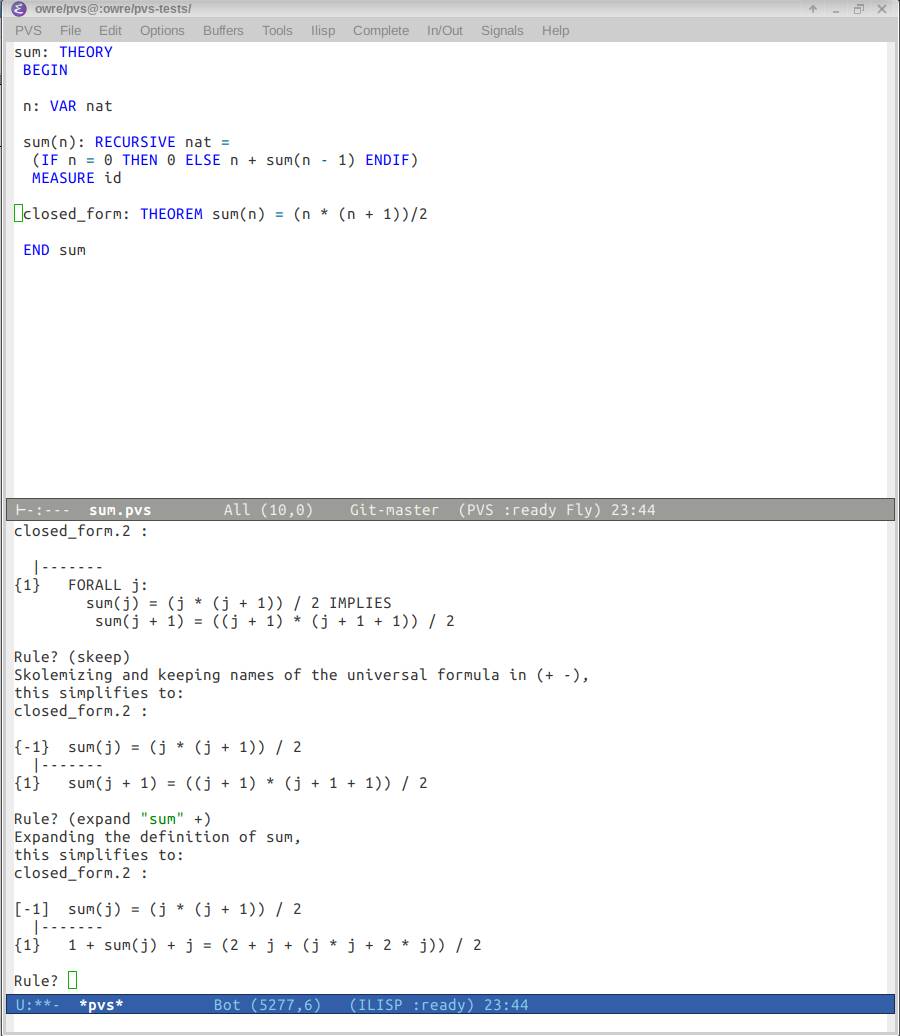
\includegraphics[width=\textwidth]{pvs-screen1.png}
\caption{The \texttt{sum} Specification in Emacs}\label{sum-screen}
\end{figure}

This simple theory has no parameters and contains three declarations.  The
first declares \texttt{n} to be a variable of type \texttt{nat}, the
built-in type of natural numbers.  The next declaration is a recursive
definition of the function \texttt{sum(n)} whose value is the sum of the
first \texttt{n} natural numbers.  Associated with this definition is a
\emph{measure} function, following the \texttt{MEASURE} keyword, which is
explained below.  The final declaration is a formula which gives the
closed form of the sum.

The \texttt{sum} theory may be introduced to the system in a number of
ways, all of which create a file with a \texttt{.pvs}
extension.\footnote{The file does not have to be named \texttt{sum.pvs}, it
simply needs the \texttt{.pvs} extension.}  The most common ways are:
\begin{enumerate}

\item Simply use \texttt{M-x find-file} (\key{C-x C-f}), or \texttt{M-x
find-pvs-file} (\ecmd{ff}, \key{C-c C-f}), provide \texttt{sum.pvs} for
the file name and type in the specification.\footnote{If there is already
a file called \texttt{sum.pvs} in the current context, this will load that
file.}

\item Use the \texttt{M-x new-pvs-file} command (\ecmd{nf}) to create a
new PVS file, and type \texttt{sum} when prompted for a file name.  Then
simply type the specification into the buffer (a basic template will be provided). 

\item Since the file is included in the distribution in the
\texttt{Examples} subdirectory of the main PVS directory, it can be
imported with the \texttt{M-x import-pvs-file} command (\ecmd{imf}).  Use
the \ecmd{whereis-pvs} command to find the path of the main PVS directory.

\item Finally, any external means of introducing a file with extension
\texttt{.pvs} into the current directory will make it available to the
system; for example, going to a \unix\ window and using \texttt{vi} to
type it in, or \texttt{cp} to copy it from the \texttt{Examples}
subdirectory.

\end{enumerate}

\section{Parsing and Typechecking}

Once the \texttt{sum} specification is displayed in the current buffer, it
can be parsed with the \iecmd{parse} (\ecmd{pa}) command, which checks the
syntactic consistency of the specification and creates the internal
abstract representation for the theory described by the specification.  If
the system finds an error during parsing, an error window will pop up with
an error message, and the cursor will be placed in the vicinity of the
error.  If you didn't get an error, introduce one (say by misspelling the
\texttt{VAR} keyword), then move the cursor somewhere else and parse the
file again---note that the buffer is automatically saved.  Fix the error
and parse once more.  In practice, the parse command is rarely used, as
the system automatically parses the specification when it needs to.

\index{typecheck|(}

The next step is to typecheck the file by typing \iecmd{typecheck}
(\iecmd{tc}, \key{C-c C-t}), which checks for semantic errors, such as
undeclared names and ambiguous types.  After \texttt{sum} has been
typechecked, a message is displayed in the minibuffer indicating that two
\tccs\index{TCCs@\tccs|(} were generated.  These \tccs\ represent
\emph{proof obligations}\index{proof obligations} that must be discharged
before the \texttt{sum} theory can be considered typechecked.  The proofs
of the \tccs\ may be postponed indefinitely, though in general it is a
good idea to view \tccs\ to convince yourself that they are provable
before moving on to other proofs in your specification.  \tccs\ can be
viewed using the \iecmd{show-tccs} (\iecmd{tccs}, \key{C-c C-q s})
command, the results of which are shown in Figure~\ref{sum-tccs} below.

\pvstheory{sum-tccs}{\tccs\ for Theory \texttt{sum}}{sum-tccs}

The first \tcc\ is due to the fact that \texttt{sum} takes an argument of
type \texttt{nat}, but the type of the argument in the recursive call to
\texttt{sum} is integer, since \texttt{nat} is not closed under subtraction.
Note that the \tcc\ includes the condition \texttt{NOT n = 0}, which holds
in the branch of the \texttt{IF-THEN-ELSE} in which the expression
\texttt{n - 1} occurs.

The second \tcc\ is needed to ensure that the function \texttt{sum} is
total, \ie\ terminates.  PVS does not directly support partial functions,
although its powerful subtyping mechanism allows PVS to express many
operations that are traditionally regarded as partial.  The measure
function is used to show that recursive definitions are total by requiring
the measure to decrease with each recursive call.

These \tccs\ are trivial, and in fact can be discharged automatically by
using the \ecmd{typecheck-prove} (\ecmd{tcp}) command, which attempts to
prove all \tccs\ that have been generated.  (Try it.)
\index{TCCs@\tccs|)}\index{typecheck|)}

\section{Proving}

We are now ready to try to prove the main theorem.  Place the cursor on
the line containing the \texttt{closed\_form} theorem, and type
\iecmd{prove} (\iecmd{pr} or \key{C-c p}).  A new buffer will pop up, the
formula will be displayed, and the cursor will appear at the
\texttt{Rule?}  prompt, indicating that the prover is ready to accept
input.  The commands needed to prove this theorem constitute only a very
small subset of the commands available to the prover.  In fact, for this
proof all that is actually needed is the single command
\texttt{(induct-and-simplify "n")}, which is a more powerful strategy.
For more information on these and other prover commands consult the prover
guide~\cite{PVS:prover}.

First, notice the display, which consists of a single formula (labeled
\texttt{\{1\}}) under a dashed line.  This is a
\emph{sequent}\index{sequent}; formulas above the dashed lines are called
\emph{antecedents}\index{antecedent} and those below are called
\emph{consequents}\index{consequent}.  The interpretation of a sequent is
that the conjunction of the antecedents implies the disjunction of the
consequents.  Either or both of the antecedents and consequents may be
empty.  An empty antecedent is equivalent to \texttt{true}, and an empty
consequent is equivalent to \texttt{false}, so if both are empty the
sequent is \texttt{false}.  Every proof in PVS starts with a single
consequent.

The basic objective of the proof is to generate a \emph{proof
tree}\index{proof tree} of sequents in which all of the leaves are
trivially true.  The nodes of the proof tree are sequents, and while in
the prover you will always be looking at an unproved leaf of the tree,
called the \emph{current} sequent.\index{current sequent} The
\emph{current} branch\index{current branch} of a proof is the branch
leading back to the root from the current sequent.  When a given branch is
complete (\ie\ ends in a proved leaf), the prover automatically moves on
to the next unproved branch, or, if there are no more unproven branches,
notifies you that the proof is complete.

Now on to the proof.  We will prove this formula by induction on
\texttt{n}.  To do this, type \texttt{(induct "n")}\index{prover
commands!induct@\texttt{induct}}.\footnote{PVS expressions are
case-sensitive, and must be put in double quotes when they appear as
arguments in prover commands.} This is not an Emacs command, rather it
is typed directly at the prompt, including the parentheses.  As indicated,
two subgoals are generated; the one displayed is the base case, where
\texttt{n} is \texttt{0}.  To see the inductive step, type
\texttt{(postpone)}\index{prover commands!postpone@\texttt{postpone}},
which postpones the current subgoal and moves on to the next unproved one.
Type \texttt{(postpone)} a second time to cycle back to the original
subgoal (labeled \texttt{closed\_form.1}).

Three extremely useful Emacs key bindings to know here are \key{M-p},
\key{M-n}, and \key{M-s}.  \key{M-p} gets the last input typed to the
prover; further uses of \key{M-p} cycle back in the input history.
\key{M-n} works in the opposite direction.  To use \key{M-s}, type the
beginning of a command that was previously input, and type \key{M-s}.
This will get the previous input that matches the partial input; further
uses of \key{M-s} will find earlier matches.  Try these key bindings out;
they are easier to use than to explain.  Thus to type the second postpone
command above, you can either type \key{M-p} or type \texttt{(po} followed
by \key{M-s}.  Section~\ref{prover-emacs} on page~\pageref{prover-emacs}
describes further useful shortcut commands for the prover.

To prove the base case, we need to expand the definition of \texttt{sum},
which is done by typing \texttt{(expand "sum")}\index{prover
commands!expand@\texttt{expand}}.  After expanding the definition of
\texttt{sum}, we issue the \texttt{(assert)}\index{prover
commands!assert@\texttt{assert}} command, which applies the decision
procedures of the prover to simplify the consequent to \texttt{TRUE},
completing the proof of this subgoal.  The prover then automatically moves
on to the next subgoal, which is the inductive step.

The first thing to do here is to eliminate the \texttt{FORALL} quantifier.
This can most easily be done with the \texttt{skolem!}\ \index{prover
commands!skolem@\texttt{skolem"!}}  command\footnote{The exclamation point
differentiates this command from the \texttt{skolem} command, where you
provide the new constant names.}, which provides new constants for the
bound variables.  To invoke this command type \texttt{(skolem!)} at the
prompt.  The resulting formula may be simplified by typing
\texttt{(flatten)}\index{prover commands!flatten@\texttt{flatten}}, which
will break up the consequent into a new antecedent and consequent.  The
obvious thing to do now is to expand the definition of \texttt{sum} in the
consequent.  This again is done with the \texttt{expand} command, but this
time we want to control where it is expanded, as expanding it in the
antecedent will not help.  So we type \texttt{(expand "sum" +)},
indicating that we want to expand \texttt{sum} in the
consequent.\footnote{We could also have specified the exact formula number
(here \texttt{1}), but including formula numbers in a proof tends to make
it less robust in the face of changes.  There is more discussion of this
in the prover guide~\cite{PVS:prover}.}

The final step is to invoke the PVS decision procedures, which can
automatically decide certain fragments of arithmetic.  This is done by
typing \texttt{(assert)}. The \texttt{assert}\index{prover
commands!assert@\texttt{assert}} command actually does a lot more than
decide arithmetical formulas, performing three basic tasks:
\begin{itemize}\def\itemsep{0in}
\item It tries to prove the subgoal using the decision procedures.

\item It stores the subgoal information in an underlying database,
allowing automatic use to be made of it later.

\item It simplifies the subgoal by rewriting (if any auto-rewrites have
been given) and by using the underlying decision procedures.
\end{itemize}
These arithmetic and equality procedures are the main workhorses of most
PVS proofs.

The proof is now complete, and is saved in the \texttt{sum.prf} file.  The
buffer from which the \cmd{prove} command was issued is then redisplayed
if necessary, and the cursor is placed on the formula that was just
proved.  The entire proof transcript is shown below.  Yours may be
slightly different, depending on your window size and the timings involved.

{\smaller\smaller
\begin{alltt}
\input{sumproof}
\end{alltt}}

A brief version of the just completed proof can be generated by the command
command \iecmd{show-last-proof}.

\section{Status}

Now type \iecmd{status-proof-theory} (\iecmd{spt}) and you will see a
buffer that displays the three formulas in \texttt{sum}, along with an
indication of their proof status.  This command is useful to see which
formulas and \tccs\ still require proofs.  Another useful command is
\iecmd{status-proofchain} (\ecmd{spc}), which analyzes a given proof to
determine its dependencies.  To use this, go to the \texttt{sum.pvs}
buffer, place the cursor on the \texttt{closed\_form} theorem, and enter
the command.  A buffer will pop up indicating that the proof is
complete, and that it depends on the \tccs\ and the \texttt{nat\_induction}
axiom, as well as some definitions and \tccs\ provided by the prelude.

\section{Generating \LaTeX}

In order to try out this section, you must have access to \LaTeX\
\index{LaTeX@\LaTeX} and a \TeX\ previewer such as
\texttt{xdvi}\index{xdvi}.

Type \iecmd{latex-theory-view} (\iecmd{ltv}).  You will be prompted for
the theory name to which you should type \texttt{sum}, or just
\texttt{Return} if \texttt{sum} is the default.  You will then be prompted
for the \TeX\ previewer name.  Either the previewer must be in your path,
or the entire pathname must be given.  This information will only be
prompted for once per session, after which PVS assumes that you want to
use the same previewer.  You can set the previewer automatically,
by adding the following line to your \texttt{\char'176/.pvsemacs} file.
{\small
\begin{alltt}
\hspace*{2em}  (setq pvs-latex-viewer "\textit{previewer}")
\end{alltt}}

\begin{figure}[ht]
\begin{center}
\begin{boxedminipage}{\textwidth}
{\small\small\input{sum-nosub}}
\end{boxedminipage}
\end{center}
\caption{Theory \texttt{sum} with default translations}\label{sum-plain}
\end{figure}

After a few moments the previewer will pop up displaying the \texttt{sum}
theory, as shown in Figure~\ref{sum-plain}.  Note that \texttt{*} has been
translated as $\times$ and \texttt{LAMBDA} as $\lambda$.  These and other
translations are built into PVS; you may also specify translations for
keywords and identifiers by providing a substitution file named
\texttt{pvs-tex.sub}, that contains commands to customize the \LaTeX\
output.  For example, if the substitution file contains the two lines
{\small\small
\begin{alltt}
    THEORY key 7 \verb|{\large\textbf{\textrm{Theory}}}|
    sum    1   2 \verb|{\sum_{i = 0}^{#1} i}|
\end{alltt}}
\noindent the output will look like Figure~\ref{sum-sub}.  See
Section~\ref{latex-output} on page~\pageref{latex-output} for more
details.

\begin{figure}[t]
\begin{boxedminipage}{\textwidth}
{\small\small\input{sum-sub}}
\end{boxedminipage}
\caption{Theory \texttt{sum} with additional translations}\label{sum-sub}
\end{figure}

\vspace*{1in}

\setcounter{footnote}{0}
% Document Type: LaTeX
% Master File: user-guide.tex
\chapter{PVS Commands}
\label{commands}
\setcounter{footnote}{0}

This chapter contains descriptions for all PVS commands; the commands are
grouped according to function.  A summary of the information in this
chapter is also provided in the buffer displayed by the \ecmd{pvs-help}
command.  The information in this chapter is best absorbed after reading
and experimenting with the brief tour provided in
Chapter~\ref{system-tutorial}.

Each of the following sections begins with a table summarizing the
commands discussed in that section; each table entry gives the full name
of the command, available aliases and/or key bindings, a brief
description, and the effect of providing command arguments.  Commands are
invoked by typing \texttt{M-x} followed by the command name or its
abbreviation, or by using a (less mnemonic) key sequence.  For example,
the \cmd{typecheck} command can be invoked by typing \ecmd{typecheck} or
one of the alternate forms \ecmd{tc} or \key{C-c C-t}.  The behavior of many
of the commands can be modified by providing an argument, and many of the
commands work on regions.\footnote{See Section 4.9 of~\cite{emacs20} for
details on providing arguments to commands, and Section 9 for creating and
manipulating regions.} For example, preceding the \cmd{typecheck} command
with a \key{C-u} or \key{M-1} forces the file to be reparsed and
typechecked, even if it has already been typechecked.  Each command that
takes an argument has a second line prefixed by \emph{Arg:} that
describes the effect of the argument.

Many PVS commands are appropriate at either the file or theory level;
yielding two different commands.  For example, the command for
creating a new PVS file is \cmd{new-pvs-file}, while the command
\cmd{new-theory} creates a template for a new theory within the current
PVS file.  In general, a command \emph{foo} that applies to both
files and theories will have a version named \ecmd{\textit{foo}-pvs-file}
and one named \ecmd{\textit{foo}-theory}.

\section{Exiting PVS}

\begin{pvscmds}
\icmd{exit-pvs} & \key{C-x C-c} & Terminate PVS session \\
\icmd{suspend-pvs} & \key{C-x C-z} & Suspend PVS \\
\end{pvscmds}

The \cmd{exit-pvs} command first saves the context information (see the
\icmd{save-context} command) and then exits PVS\@.  If there is a proof in
progress, the system will not exit, but will instead output a message
asking you to exit the prover, thus giving you the opportunity to save the
proof before exiting.

The \cmd{suspend-pvs} command suspends the Emacs process, except under
X-windows, where the command has no effect.  The system first asks whether
the context should be saved; if you answer \texttt{yes} the
\icmd{save-context} command is invoked prior to suspending PVS.  This may
take a while, as the \cmd{save-context} may have to save any number of
files, depending on what has changed in the context.  The suspended job
can be restarted from the \unix\ shell in which it was suspended by first
determining the job number (using the \unix\ command ``\texttt{jobs}'')
and then typing ``\texttt{fg \%$n$}'', where $n$ is the job
number.\footnote{This assumes you are running the \texttt{csh} or
\texttt{tcsh} shell. To restart under a shell lacking job control, use the
\unix\ command \texttt{ps} to determine the process id ($pid$) and then do
\texttt{kill -CONT pid}.}

\section{Getting Help}
\begin{pvscmds}
\icmd{help-pvs}, \icmd{pvs-help} & \key{C-c h} & Display the PVS help
  buffer \\
\icmd{help-pvs-bnf}, \icmd{pvs-help-bnf} & \key{C-c C-h b} & Display the
  pvs grammar \\
\icmd{help-pvs-language}, & \key{C-c C-h l} & Display help for the PVS
  language \\
\quad\icmd{pvs-help-language} & & \\
\icmd{help-pvs-prover}, & \key{C-c C-h p} & Display help for the prover
  commands \\
\quad\icmd{pvs-help-prover} & & \\
\icmd{help-pvs-prover-command}, & \key{C-c C-h c} &
  Display help for prover command \\
\quad\icmd{pvs-help-prover-command} & & \\
\icmd{help-pvs-prover-strategy}, & \key{C-c C-h s} &
  Displays the specified prover strategy \\
\quad\icmd{pvs-help-prover-strategy} & & \\
\icmd{x-prover-commands} & & Displays the prover commands in a \\
& & \quad Tcl/Tk window \\
\icmd{help-pvs-prover-emacs}, & \key{C-c C-h e} &
  Display help for prover emacs commands \\
\quad\icmd{pvs-help-prover-emacs} & & \\
\icmd{pvs-release-notes}, & \key{C-c C-h r} & Display PVS release notes \\
\end{pvscmds}

The \cmd{help-pvs} command displays a summary of PVS commands in the
\ibuf{PVS Help} buffer.  Help may be obtained for an individual command by
typing \texttt{C-h f} followed by the command or its abbreviation, or by
typing \texttt{C-h k} followed by the key sequence that invokes the
command.  These are built in to Emacs, and may be used to get help for
any Emacs command or key sequence, not just PVS commands.

The \cmd{help-pvs-bnf} command provides the PVS grammar in BNF form, and
the \cmd{help-pvs-language} command displays a summary of the PVS language
with examples in the \ibuf{Language Help} buffer.

The \cmd{help-pvs-prover} command displays the documentation string for
all of the prover commands in the \ibuf{Prover Help} buffer.  The
\cmd{help-pvs-prover-command} displays the documentation string for the
specified command, and the \cmd{help-pvs-prover-strategy} command provides
the arguments, definition, format string, and documentation string for the
specified command.  The latter is useful for finding out exactly what a
strategy does, or for defining your own strategies based on existing ones.
If you are running under the X window system, \icmd{x-prover-commands}
provides an easy interface to get help for individual prover commands.

The \cmd{help-pvs-prover-emacs} command displays a summary of the commands
that provide a convenient Emacs interface to the PVS prover.  This is
discussed in more detail in Section~\ref{prover-emacs},
page~\pageref{prover-emacs}.  The help text appears in the \ibuf{Prover
Emacs Help} buffer.

The \cmd{pvs-release-notes} command displays the release notes for the
running version of PVS.  The text appears in the \ibuf{PVS Release Notes}
buffer.

\section{Editing PVS Files}

\begin{pvscmds}
\icmd{forward-theory} & \key{M-\char125} & Move forward to beginning of next theory \\
\icmd{backward-theory} & \key{M-\char123} & Move backward to beginning of previous theory \\
\icmd{find-unbalanced-pvs} & \key{C-c ]} & Find unbalanced delimiters \\
\icmd{comment-region} & \key{C-c ;} & Comment out all lines in the current region \\
 & & \emph{Arg:} Uncomment all lines in the current region\\
\end{pvscmds}

PVS specification files are edited using the standard Emacs editing
commands.  Appendix~\ref{emacs-intro}, page~\pageref{emacs-intro} gives a
brief introduction to the most useful Emacs commands for editing PVS
files.

The \cmd{forward-theory} and \cmd{backward-theory} commands are used to
move to different theories within a single PVS file.  The cursor is
moved to the beginning of a theory; if there are no preceding or
following theories to move to, the message ``\texttt{No more theories}''
or ``\texttt{No earlier theories}'' is displayed and the cursor remains unchanged.

The \cmd{find-unbalanced-pvs} command checks whether there are any
unbalanced parentheses (\texttt{( )}), square brackets (\texttt{[ ]}), curly
braces (\verb|{ }|), or \texttt{BEGIN-END} pairs.  If none are found, the
message ``\texttt{All delimiters balance}'' is displayed.  Otherwise the
cursor is left at the token for which there is no match and a
corresponding message is displayed.

The \cmd{comment-region} command inserts the comment character
(\texttt{\%}) at the beginning of every line in the specified region.  To
uncomment a region, simply provide an argument to the command, and all
commented lines within the region will be uncommented.

\section{Parsing and Typechecking}

\subsection{Parsing}

\begin{pvscmds}
\icmd{parse} & \icmd{pa} & Parse file in current buffer \\
             & & \emph{Arg:} Forces the file to be reparsed \\
\end{pvscmds}

Parsing a PVS specification accomplishes two things: first, it checks that
the specification is syntactically correct, \ie\ satisfies the PVS
grammar, and second, it builds the internal abstract grammar data
structures.  The \cmd{parse} command is not normally used, as typechecking
will automatically parse the file if required.  Note that only files (with
extension \texttt{.pvs}) may be parsed.  When a file is parsed, it becomes a
part of the context if it wasn't already, and any proofs that have been
saved for the file are reinstated.  If the file being parsed has a valid
\texttt{.bin} file, then this file is loaded instead (this will result in
the file being typechecked as well as parsed).

Parsing is invoked by moving the cursor to a buffer containing a file in
the current context, and issuing the \cmd{parse} command.  While parsing
the file, the minibuffer displays the message ``\texttt{Parsing
\textit{foo}}.''  If there is no error, the message ``\texttt{\textit{foo}
parsed in \textit{\#} seconds}'' is displayed.  If the file has not changed
since the last time it was parsed, the message ``\texttt{\textit{foo} is
already parsed}'' is displayed.  To force reparsing, provide an argument
to the parse command.  Note that the argument is usually not needed, as
changes to the file are automatically detected by the system and the file
is reparsed in that case.

When an error is detected, the file is displayed with the cursor at the
location where the error was detected, which is frequently after the
actual source of the error.  In addition, the \ibuf{PVS Error} buffer is
displayed with an explanatory error message.  You may need to consult the
language manual for details on the grammar.

Certain language features may result in the parser producing theory
messages.  See the \cmd{show-theory-messages} command
(page~\pageref{tc-info}) for details.


\subsection{Typechecking}

\begin{pvscmds}
\icmd{typecheck} & \icmd{tc}, \key{C-c C-t} & Typecheck theories in current buffer \\
& & \emph{Arg:} Force reparsing and retypechecking \\
\icmd{typecheck-importchain} & \icmd{tci} & Typecheck importchain of theories \\
& & \emph{Arg:} Force reparsing and retypechecking \\
\icmd{typecheck-prove} & \icmd{tcp} & Typecheck theories, proving \tccs \\
& & \emph{Arg:} Force reparsing and retypechecking \\
\icmd{typecheck-prove-importchain} & \icmd{tcpi} & Typecheck importchain
of theories,\\ & &  proving \tccs \\
& & \emph{Arg:} Force reparsing and retypechecking \\
\end{pvscmds}

Typechecking a PVS specification checks semantic constraints, determines
the types of expressions, and resolves names (see the language
manual~\cite{PVS:language}).  Typechecking\cmdindex{typecheck} is invoked
much like parsing, and automatically parses the file if necessary.  Errors
are indicated in the same manner as for parsing, although the cursor is
usually more accurately positioned at the error.  As in parsing, an
argument to the command forces reparsing and retypechecking.  Without the
argument, \cmd{typecheck} and \cmd{typecheck-importchain} are the same.
With the argument, \cmd{typecheck} only reparses and retypechecks the
current file, while \cmd{typecheck-importchain} forces reparsing and
retypechecking of the entire import chain of the theories of the current
file.

Forcing a file to be retypechecked is done primarily for development and
debugging, as is the case for reparsing.  If you have typechecked a set of
PVS files, made some changes and found an error on retypechecking that
shouldn't have occurred, try forcing a typecheck of the file where the
error occurred.  If that doesn't help, try forcing with
\cmd{typecheck-importchain}.  The error should disappear after that,
unless it is a true typecheck error.  If it is not a simple typecheck
error, send a bug report to \texttt{pvs-bugs@csl.sri.com}.

The typechecker will attempt to typecheck any theories
appearing in \texttt{IMPORTING} clauses.  If the theories appear in the
current context, then the associated file is typechecked, otherwise
PVS tries to find a file with the same name as the theory.  For
example, in typechecking
\begin{alltt}
  IMPORTING foo[int]
\end{alltt}
the current context (reflected in the context file \texttt{.pvscontext}) is
searched for a file known to contain theory \texttt{foo}.  If no such file is
found, then the file \texttt{foo.pvs} is sought.  If that also cannot be
found, the system complains and the desired file must be manually
located (or created) and typechecked.

The \cmd{typecheck-prove} command typechecks the file, and then attempts
to prove the generated \tccs.  If the file is already typechecked, but the
\tcc\ proofs have not yet been attempted, then they are attempted in the
order they were generated.  The \tcc\ proof attempts are made with 
built-in prover strategies (selected according to the type of \tcc\
generated). These strategies basically expand all
definitions in the \tcc, and repeatedly skolemize, perform heuristic
instantiation, lift \texttt{IF}s, and invoke the decision
procedures.\footnote{The TCC strategies are variants of a powerful
strategy called \texttt{(grind)}, which is useful for more
than just \tccs.} As explained in the prover guide, you may redefine the
\texttt{tcc} strategies; usually to extend their capabilities.

The \cmd{typecheck-prove-importchain} command typechecks the file, and
attempts to prove the \tccs\ of all the theories on the import chain that
have not already been attempted.  Providing an argument forces the
retypechecking of the import chain.

The \cmd{typecheck-prove} commands can take some time, especially if there
are a lot of \tccs.  This can be controlled in a number of ways:
\begin{description}

\item[Use these commands sparingly.] Our experience is that \tccs\ should
be analyzed whenever a new specification is created, significantly
modified, or is nearing completion. 
At these times it pays to use the \cmd{typecheck-prove} command and
to look at the \tccs\ that weren't subsequently proved, and check that
they at least seem provable.
After minor changes, we find it best to use just \cmd{typecheck} and
defer consideration of the \tccs\ until later.


\item[Define your own \tcc\ strategy.] The prover guide describes
techniques for defining your own strategies, and you may change existing
ones, such as the \texttt{tcc} strategy to be more efficient for your
particular specifications.  Changing the \texttt{tcc} strategy should
probably be done in the \texttt{pvs-strategies} file in the current
context, especially if it is tailored to the specifications in that
context.

\item[Use judgements\index{judgements} to cut down on the number of
  \tccs.]  The language manual describes \newline
  how to do this.

\item[Use \texttt{NONEMPTY\_TYPE} or \texttt{CONTAINING} in type
declarations]  This is also described in the language manual.

\end{description}

When typechecking is completed, a message is displayed, indicating the
total number of \tccs\ generated along with a breakdown of the number
proved, subsumed\footnote{A \tcc\ is subsumed if there is an earlier
\tcc\ which implies it.  PVS uses a simple syntactic test, so not all
possible subsumptions will be determined.}, and unproved.

\subsection{Typechecking Information}
\label{tc-info}

\begin{pvscmds}
\icmd{show-theory-warnings} & & Show typechecker warnings for the given theory \\
\icmd{show-pvs-file-warnings} & & Show typechecker warnings for the given file \\
\icmd{show-theory-messages} & & Show typechecker messages for the given theory \\
\icmd{show-pvs-file-messages} & & Show typechecker messagess for the given file \\
\icmd{show-theory-conversions} & & Show conversions for the given theory \\
\icmd{show-pvs-file-conversions} & & Show conversions for the given file \\
\end{pvscmds}

\index{Conversion} \index{typechecker warnings}
\index{typechecker messages}

In the process of typechecking a specification, various warnings and
informative messages may be produced.  These are associated with the
theory that produced them, and saved so they may be perused.  Warnings may
indicate a possible problem.  For example, if the typechecker cannot
determine that a datatype is nonempty, it produces a warning.  There is
nothing wrong with having an empty datatype, but if at some point it isn't
proved to be nonempty, a lot of time may be wasted proving formulas that
are vacuously true.  Informative messages do not indicate anything is
wrong, but the information may be of interest.  For example, using the
\texttt{TYPE+} keyword generates an existence axiom, and this is treated
as an informative message.

Conversion messages\footnote{See the Language Guide\cite{PVS:language} for
details of conversions.} have been separated out of the warnings.
Conversions may be applied to make an expression type correct.  This is
not always what the user intended, so the show conversions commands are
provided to make it easy to look at the conversions that have been applied.

Note that typechecking not only reports the number of \tccs\ generated,
but also the generation of any warnings, messages, and conversions.  While
in the prover, these messages are generated interactively.


\section{Proving}

The prover\index{prover} is described in full in the prover
guide~\cite{PVS:prover}, here we describe the Emacs interface to the
prover, including commands for invoking the prover, editing and rerunning
proofs, displaying proof information, some useful keyboard shortcuts for
the prover, and managing multiple proofs.

The prover may be applied to a single formula, all formulas in a theory,
all formulas in the import chain of a theory, all formulas in a PVS
file, or all formulas in the proof chain of a given formula.  Only the
\cmd{prove}, \cmd{x-prove}, \cmd{step-proof} and \cmd{x-step-proof}
commands lead to prover interaction; the other commands
simply rerun proof scripts that have been previously generated.

PVS keeps track of the status of formulas within and across sessions.  The
status may be one of four values; ``untried'' means that no proof has been
attempted, ``proved'' means that the proof has been completed,
``unchecked'' means that a proof has been completed, but that the
specification has been modified since the proof attempt, and
``unfinished'' means that a proof has been attempted, but not yet
completed.  Formulas labelled as ``proved'' will be ``complete'' or
``incomplete''.  The status is only ``complete'' when all formulas
(including \tccs) upon which the proof is dependent have been completed.

Modifying a specification causes the proof status of all proved formulas
to revert to ``unchecked,'' although the proof scripts are
retained.\footnote{PVS currently tracks the consequences of changes rather
coarsely: any change in a file reverts all the proofs in that file, and
all those in theories that depend on that file (and so on, transitively)
to the ``unchecked'' state.}
\subsection[Proving a Single Formula]{Proving a Single Formula}
\label{prove-commands}

\begin{pvscmds}
\icmd{prove} & \icmd{pr}, \key{C-c p} & Prove formula pointed to by cursor
\\
\icmd{x-prove} & \icmd{xpr}, \key{C-c C-p x} & Start proof along with X
display \\
\icmd{step-proof} & \icmd{prs}, \key{C-c C-p s} & Set up proof stepper for
current formula \\
\icmd{x-step-proof} & \icmd{xsp}, \key{C-c C-p X} & Combines \cmd{x-prove} and \cmd{step-proof} \\
\icmd{redo-proof} & \icmd{prr} \key{C-c C-p r} & Redo the proof of formula at cursor \\
 & & \emph{Arg:} don't display the proof \\
\multicolumn{2}{|l}{
\icmd{prove-next-unproved-formula}} & \\
& \icmd{prnext}, \key{C-c C-p n} & Start proof on next unproved formula
\\
\end{pvscmds}

To invoke the prover on a single formula, move the cursor to any part of
the desired formula and type the \cmd{prove} command.  The formula may be
in a PVS file, a buffer generated by the \cmd{prettyprint-expanded}
command (with extension \ibuf{.ppe}), a buffer generated by the
\cmd{show-tccs} command (with extension \ibuf{.tccs}), or a prelude buffer
produced by one of the \texttt{view-prelude} commands.\footnote{Of course,
the prelude formulas have already been proved; this facility allows you to
explore the proofs.}  If the formula has already been proved, then you
will be asked whether the proof should be retried; a \texttt{no} answer
ends the \cmd{prove} command.  Otherwise, if the formula has an associated
proof script, you will be asked whether to rerun the proof or start over.
In either of these two cases, the proof is displayed in the \ibuf{*pvs*}
buffer.  If the proof script terminates before completing the proof or if
no script was requested, the prover will prompt for a command, which
should be typed directly into the \buf{*pvs*} buffer at the \texttt{Rule?}
prompt.\footnote{The system tries to keep as much of the proof visible as
possible by redisplaying the screen so that the \texttt{Rule?}\ prompt is
at the bottom of the window.  This feature is not always desirable (\eg\
over a slow modem connection), and may be turned off by setting the Emacs
variable \texttt{*pvs-maximize-proof-display*} to nil.}  At this point you
are interacting with the prover, and certain commands will be unavailable
until the prover is exited.\footnote{\label{prover-restrictions}
Specifically, the commands \cmd{parse}, \cmd{typecheck}, \cmd{prove},
\cmd{change-context}, \cmd{exit-pvs}, and all of the prove commands of
this section are unavailable while the prover is active.}

The \cmd{x-prove} command is exactly like the \cmd{prove} command, except
that it also pops up a window in which the proof tree is represented
graphically.  See section~\ref{display-commands},
page~\pageref{display-commands} for more details.  If you are not running
under X windows, then a warning message will be displayed and the command
will be treated as a \cmd{prove} command.

The \cmd{step-proof} command is used to initiate the proof stepper, and is
invoked in the same way as the \cmd{prove} command.  Two buffers are
displayed, one showing the sequent (the \ibuf{*pvs*} buffer) and the other
showing the proof script associated with the formula, if any (the
\ibuf{Proof} buffer).  Section~\ref{proof-stepper},
page~\pageref{proof-stepper} explains how to use the proof stepper.

The \cmd{x-step-proof} command combines the \cmd{x-prove} and
\cmd{step-proof} commands.

The \cmd{prove-next-unproved-formula} command invokes the prover on the
next unproved formula at or beyond the current cursor position.  If the
formula already has a proof, you will be asked whether to go ahead and run
it or to start anew.  Note that starting a new proof will not delete the
old proof unless you allow the prover to overwrite it at the end of the
proof session.

The \cmd{redo-proof} command is invoked exactly like the \cmd{prove}
command, but simply reruns the proof with no questions asked.  An
error is signaled if the indicated formula has no associated proof.
In addition, if an argument is provided, the proof will not be
displayed interactively---instead the proof is processed in the
background, and the status of the proof is provided in the minibuffer
when the attempt is completed.

The prover exits automatically when a proof is successfully completed.  If
at any time you want to exit the prover, go to the bottom of the
\ibuf{*pvs*} buffer\footnote{While in the prover you may freely move
around in the \ibuf{*pvs*} buffer or move to any other buffer to examine
specifications or perform ordinary editing functions.} and type
\texttt{(quit)} to the \texttt{Rule?}\ prompt.  If there is no such
prompt, type \key{C-c C-c} and \texttt{(restore)} to get to the prompt.
Once the prover is exited, control is returned to the buffer from which
the prover was invoked, with the cursor positioned at the beginning of the
formula being proved.  Do not kill the \ibuf{*pvs*} buffer, as
this will also kill the associated PVS process.

\subsection[Proving Sets of Formulas]{Proving Sets of Formulas}
\begin{pvscmds}
\icmd{prove-theory}
  & \icmd{prt}, \key{C-c C-p t}
  & Rerun unproved proofs in theory \\
 & & \emph{Arg:} include those already proved \\
\icmd{prove-theories}
  &
  & Rerun proofs in specified theories \\
 & & \emph{Arg:} include those already proved \\
\multicolumn{2}{|l}{
\icmd{prove-pvs-file}}
  & Rerun unproved proofs in current file \\
 & \icmd{prf}, \key{C-c C-p f}
 & \emph{Arg:} include those already proved \\
\multicolumn{2}{|l}{
\icmd{prove-importchain}}
  & Rerun prove-theory on \texttt{IMPORT} chain \\
 & \icmd{pri}, \key{C-c C-p i}
 & \emph{Arg:} include those already proved \\
\multicolumn{2}{|l}{
\icmd{prove-importchain-subtree}}
  & Rerun prove-theory on specified subtree \\
  & \icmd{pris} & of \texttt{IMPORT} chain \\
 & & \emph{Arg:} include those already proved \\
\multicolumn{2}{|l}{
\icmd{prove-proofchain}}
  & Rerun proofs on formulas in proofchain \\
 & \icmd{prp}, \key{C-c C-p p}
 & \emph{Arg:} include those already proved \\
\multicolumn{2}{|l}{
\icmd{prove-formulas-theory}}
  & Try unproved formulas with specified strategy \\
 & \icmd{prft}
 & \emph{Arg:} attempt proved formulas as well \\
\multicolumn{2}{|l}{
\icmd{prove-formulas-pvs-file}}
 & Try unproved formulas with specified strategy \\
 & \icmd{prff}, \key{C-c C-p U}
 & \emph{Arg:} attempt proved formulas as well \\
\multicolumn{2}{|l}{
\icmd{prove-formulas-importchain}}
 & Try unproved formulas with specified strategy \\
 & \icmd{prfi} & \emph{Arg:} attempt proved formulas as well \\
\multicolumn{2}{|l}{\cmd{prove-formulas-importchain-subtree}\cmdindex{prove-formulas-importchain- \newline subtree}} \\
 & Try unproved formulas with specified strategy \\
 & \icmd{prfs} & \emph{Arg:} attempt proved formulas as well \\
\multicolumn{2}{|l}{
\icmd{prove-tccs-theory}}
  & Try unproved TCCs with specified strategy \\
 & \icmd{prft}
 & \emph{Arg:} attempt proved TCCs as well \\
\multicolumn{2}{|l}{
\icmd{prove-tccs-pvs-file}}
  & Try unproved TCCs with specified strategy \\
 & \icmd{prff}, \key{C-c C-p U}
 & \emph{Arg:} attempt proved TCCs as well \\
\multicolumn{2}{|l}{
\icmd{prove-tccs-importchain}}
 & Try unproved TCCs with specified strategy \\
 & \icmd{prfi} & \emph{Arg:} attempt proved TCCs as well \\
\multicolumn{2}{|l}{
\icmd{prove-tccs-importchain-subtree}}
 & Try unproved TCCs with specified strategy \\
 & \icmd{prfs} & \emph{Arg:} attempt proved TCCs as well \\
\multicolumn{2}{|l}{
\icmd{prove-untried-theory}}
  & Try untried proofs with specified strategy \\
 & \icmd{prut}, \key{C-c C-p u}
 & \emph{Arg:} attempt TCCs as well \\
\multicolumn{2}{|l}{
\icmd{prove-untried-pvs-file}}
  & Try untried proofs with specified strategy \\
 & \icmd{pruf}, \key{C-c C-p U}
 & \emph{Arg:} attempt TCCs as well \\
\multicolumn{2}{|l}{
\icmd{prove-untried-importchain}}
 & Try untried proofs with specified strategy \\
 & \icmd{prui} & \emph{Arg:} attempt TCCs as well \\
\multicolumn{2}{|l}{
\icmd{prove-untried-importchain-subtree}}
 & Try untried proofs with specified strategy \\
 & \icmd{prus} & \emph{Arg:} attempt TCCs as well \\
\end{pvscmds}
Proof scripts can be rerun using the \cmd{prove-theory},
\cmd{prove-pvs-file}, \cmd{prove-importchain},
\cmd{prove-importchain-subtree} and \cmd{prove-proofchain} commands, which
simply rerun the proof scripts, if any, for all of the formulas of the
theory, its PVS file, import chain\index{import chain}, import chain
subtree\index{import chain subtree}, or proof chain\index{proof chain},
respectively.  The import chain of a theory is simply the transitive
closure of the \texttt{IMPORTING}s including those implicit in a theory
declaration.  The \cmd{prove-importchain-subtree} command takes additional
theory name arguments and excludes these theories and their subtree from
the importchain.  The proof chain of a given formula is the transitive
closure of the formulas used in the proof of that formula.  These
commands skip formulas that have no proof scripts, and normally skip
formulas which already have status ``proved;'' providing an argument to
the command forces PVS to reprove all formulas that have proof scripts.
When any of these commands finish processing, the corresponding proof
status command\index{proof status commands} is automatically invoked to
display the results (see Section~\ref{proof-status}).

The \cmd{prove-theories} command prompts for theory names (with
completion) one at a time, until an empty theory name is provided, and
then runs \cmd{prove-theory} on each of these.


The commands
\begin{itemize}\setlength{\topsep}{0pt}\setlength{\parskip}{0pt}%
  \setlength{\itemsep}{0pt}\setlength{\parsep}{0pt}\renewcommand{\labelitemi}{}
\item \cmd{prove-formulas-theory},
\item \cmd{prove-formulas-pvs-file},
\item \cmd{prove-form\-ulas-importchain},
\item \cmd{prove-formulas-importchain-subtree},
\item \cmd{prove-tccs-theory},
\item \cmd{prove-tccs-pvs-file},
\item \cmd{prove-tccs-importchain},
\item \cmd{prove-tccs-importchain-subtree},
\item \cmd{prove-untried-theory},
\item \cmd{prove-untried-pvs-file},
\item \cmd{prove-untried-importchain}, and
\item \cmd{prove-untried-importchain-subtree}
\end{itemize}
are all similar, but allow a
given strategy to be applied to all applicable formulas.

For the \cmd{prove-formulas} commands, all unproved formulas that are not
TCCs or axioms or postulates are attempted with the provided strategy,
which defaults to \texttt{(grind)}.  The \cmd{prove-tccs} commands are
similar, but only attempt unproved TCCs, and the default strategy is
\texttt{(tcc)}.  With an argument, the already proved formulas are also
attempted.  If a given proof attempt succeeds, then it replaces any
existing proof.  If it fails and the given formula already has a proof,
then the original proof is kept.  Otherwise the new proof is associated
with the formula.  Thus after these commands all attempted formulas will
have proofs associated with them.  The strategy is any acceptable single
prover command, as in the following example.
\begin{alltt}
  (then (grind :if-match nil) (inst?) (grind))
\end{alltt}

The \cmd{prove-untried} commands are similar, but they only affect
formulas that have no associated proof, and providing an argument attempts
TCCs that have no proofs as well.  To apply a strategy to just the untried
TCCs, redefine the \texttt{tcc}\index{tcc strategy@\texttt{tcc} strategy}
in your \texttt{pvs-strategies}\index{pvs-strategies file}
Note that after any of these commands,
all attempted formulas will have associated proofs, so issuing the same
command with a different strategy will have no effect.

\glossary{[import chain:] the transitive closure of the \texttt{IMPORTING}s
of a theory}
\glossary{[proof chain:] the transitive closure of the formulas
used in the specified proof}

\subsection{Selecting Decision Procedures}
\label{decision-procedure-commands}

\begin{pvscmdsna}
\multicolumn{2}{|l|}{\icmd{set-decision-procedure}} \\
  & Set the default decision procedure \\
\multicolumn{2}{|l|}{\icmd{prove-theory-using-default-dp}} \\
  & Rerun unproved proofs in specified theory using default decision procedures\\
 & \emph{Arg:} include those already proved \\
\multicolumn{2}{|l|}{\icmd{prove-theories-using-default-dp}} \\
  & Rerun proofs in specified theories using default decision procedures\\
 & \emph{Arg:} include those already proved \\
\multicolumn{2}{|l|}{\icmd{prove-pvs-file-using-default-dp}} \\
 & Rerun unproved proofs in current file using 
  default decision procedures \\
 & \emph{Arg:} include those already proved \\
\multicolumn{2}{|l|}{\icmd{prove-importchain-using-default-dp}} \\
  & Rerun prove-theory on \texttt{IMPORT} chain using
    default decision procedures \\
 & \emph{Arg:} include those already proved \\
\multicolumn{2}{|l|}{\cmd{prove-importchain-subtree-using-default-dp}\cmdindex{prove-importchain-subtree-using- \newline default-dp}} \\
  & Rerun prove-theory on subtree of \texttt{IMPORT}
  chain using default dec. procedures \\
 & \emph{Arg:} include those already proved \\
\multicolumn{2}{|l|}{\icmd{prove-proofchain-using-default-dp}} \\
 & Rerun proofs on all formulas in proof chain using default decision procedures \\
 & \emph{Arg:} include those already proved \\
\end{pvscmdsna}

\emph{These commands have no effect if PVS was invoked with the
\texttt{\textrm{-force-decision-procedures}} switch; see
Section~\ref{invoking-pvs}}

The currently available decision procedures are \texttt{shostak} and
\texttt{ics}.  Much of the prover was built around the Shostak decision
procedure,\footnote{This was developed by Rob Shostak in the late 70s.
Since then it has undergone many refinements.}  ICS is a new decision
procedure that can be run stand alone or included as a library.  See
\url{http://ics.csl.sri.com} for more.  The prover manual discusses how
the decision procedures are used; here we simply describe the commands for
selecting them.

The decision procedure interface provides a set of methods that make it
easy to add new decision procedures, as long as they satisfy the basic
API.  When a new decision procedure is added, it's name is made available
to be used as a decision procedure.

The \cmd{set-decision-procedure} command sets the default decision
procedure to be used in subsequent proofs.  When a single formula is
attempted that doesn't have a proof, the default decision procedure is
automatically used.  If it already has a proof that was developed using
a different decision procedure, the prover prompts for whether to use the
default or stay with the original decision procedure.  When a proof is
saved, the decision procedure used during the proof is saved as well.  For
the prover commands such as \cmd{prove-theory}, the proofs are each
attempted with the decision procedure they were developed with.  The
remaining commands allow existing proofs to be rerun using the default
decision procedures, and otherwise behave exactly as the similarly named
commands defined in the previous section.

Note that setting the decision procedure does not affect an ongoing
proof.  The decision procedures generally have different ways of storing
state and processing it, and a proof may only be run with a single
decision procedure.  However, the decision procedure API is flexible
enough to allow methods to be defined that, for example, run two different
decision procedures in parallel and compare their results, or spawn two
subprocesses and use the result of the first one to finish.

\subsection{Editing and Viewing Proofs}

\begin{pvscmds}
\icmd{edit-proof} & \icmd{show-proof} & Edit the proof of the indicated
formula \\
\icmd{install-proof} & \key{C-c C-i} & Install proof on the indicated formula \\
\icmd{install-and-step-proof} & \key{C-c s} & Install proof on a formula and step \\
\icmd{install-and-x-step-proof} & \key{C-c x} & Install proof on formula, display, and step \\
\icmd{remove-proof} & & Remove proof associated with a formula \\
\icmd{show-proof-file} & & Edit the proofs of the indicated PVS file \\
\icmd{show-orphaned-proofs} & & Edit the orphaned proofs \\
\icmd{show-proofs-theory} & & Show all proofs of a theory \\
\icmd{show-proofs-pvs-file} & & Show all the proofs of a PVS file \\
\multicolumn{2}{|l}{\icmd{show-proofs-importchain}} & Show all proofs of importchain of
a theory \\
\multicolumn{2}{|l}{\icmd{install-pvs-proof-file}} & Installs proof file
for typechecked theory \\
\icmd{display-proofs-formula} & & Display the (multiple) proofs associated
with this formula \\
\icmd{display-proofs-theory} & & Display the (multiple) proofs of the
formulas in the theory \\
\icmd{display-proofs-pvs-file} & & Display the (multiple) proofs of the
formulas in the PVS file \\
\icmd{load-pvs-strategies} & & Loads a pvs-strategies file \\
\icmd{set-print-depth} & & Sets print depth for printing sequents \\
\icmd{set-print-length} & & Sets print length for printing sequents \\
\icmd{set-print-lines} & & Sets number of lines to print \\
 & & \quad for each sequent formula \\
\icmd{set-rewrite-depth} & & Sets the print depth for rewrite messages \\
\icmd{set-rewrite-length} & & Sets the print length for rewrite messages \\
\icmd{dump-sequents} & & Save unproved sequents to a file \\
\multicolumn{2}{|l}{\icmd{toggle-proof-prettyprinting}} & Toggles the prettyprinting of proof
files \\
\end{pvscmds}

Every formula of a specification for which a proof has been attempted has
an associated proof script that reflects the commands used during the
proof attempt.  Proof scripts may be edited using the \cmd{edit-proof}
command.  This command is invoked on the formula declaration at the
cursor; the formula may occur in a specification buffer (with extension
\ibuf{.pvs}), a prettyprint-expanded buffer (with extension \ibuf{.ppe}),
a show-tccs buffer (with extension \ibuf{.tccs}), or a buffer generated by
one of the \texttt{view-prelude} commands.  When the \cmd{edit-proof}
command is invoked, it creates a buffer with the name \ibuf{Proof}
containing the relevant proof script,\footnote{If the formula has no proof
script, an empty \ibuf{Proof} buffer is created.}  which may then be
edited using the standard Emacs editing commands.  Editing proof scripts
is a convenient way to handle modifications made to a specification, and
allows the same proof script to be revised and used for many similar
formulas.  The \ibuf{Proof} buffer normally persists until the next time
the \cmd{edit-proof} command is invoked, allowing the same proof script to
be attached to different formulas using \icmd{install-proof}.

A proof script records a tree of prover commands that will generate a
proof of the given formula.  Although the proof tree does not record
verbatim the commands originally typed to the prover, the proof script
should be easy to understand.  For example, the \ibuf{Proof} buffer of
the formula \texttt{closed\_form} in the \texttt{sum} example would
contain

{\small\small
\begin{alltt}
  ;;; Proof for formula sum.closed_form
  ;;; developed with old decision procedures
  (""
   (INDUCT "n")
   (("1" (EXPAND "sum") (ASSERT))
    ("2" (SKOLEM!) (FLATTEN) (EXPAND "sum" +) (ASSERT))))
\end{alltt}}

When editing is complete, the proof script may be attached either to the
original, or to a different formula using the \cmd{install-proof} command.
If this command is invoked in the \ibuf{Proof} buffer, it attaches the new
proof script to the original formula and offers to rerun the proof.  The
proof script may also be attached to any other formula by invoking
\cmd{install-proof} in a \ibuf{.pvs}, \ibuf{.ppe}, or \ibuf{.tccs} buffer,
in which case the script is attached to the formula at the cursor.  In
each case, the new proof only becomes the default, the old proofs are
still available and may be manipulated by means of the
\cmd{display-proofs-formula} command, which allows the default proof to be
reset.  If no proof is being edited (\ie\ there is no \ibuf{Proof}
buffer), an error is reported.

The proof may also be installed using the \cmd{install-and-step-proof} or
\cmd{install-and-x-step-proof} commands, both of which install the proof
and initiate the proof stepper; the latter also displays the proof tree.

Checkpoints may be added to the \texttt{Proof} buffer obtained by the
\texttt{edit-proof} command.  To add a checkpoint, position the cursor and
type \texttt{C-c a}.  The checkpoint is indicated by a double exclamation
point (\texttt{!!}).  Any number of checkpoints may be added.  When the
proof is installed using \texttt{C-c C-i}, these are changed to the
\texttt{checkpoint} proof rule, and branches of the proof that do not have
a checkpoint on them are wrapped in a \texttt{just-install-proof} proof
rule.  When this proof is rerun, it will run until it hits a
\texttt{checkpoint}, and then prompt for a prover command.  When it hits a
\texttt{just-install-proof}, it simply installs the given commands and
marks that branch as proved.  This allows the prover to quickly get to the
next checkpoint, without attempting to reprove branches that do not have
checkpoints in them.  When a proof that has \texttt{just-install-proof}
rules in it is finished, the prover asks whether the proof should be
rerun, as the formula will not be considered proved until the proof is
rerun.

To remove a checkpoint from the \texttt{Proof} buffer, position the cursor
at the checkpoint and type \texttt{C-c r}.  To remove all checkpoints,
type \texttt{C-c DEL}.

In addition to the above, the key bindings for browsing and the prover
emacs (\textsc{tab}) commands are available in a \texttt{Proof} buffer.

The \cmd{remove-proof} command is used to remove the proof associated with
the specified formula.  The primary use for this is to remove proofs from
axioms for which a proof attempt has been made.

If a proof is in progress, proofs may still be edited, but the prover must
be exited before the edited proof may be attached to a formula.  Note that
invoking \icmd{edit-proof} on the formula currently being proved will
display the proof script stored with the formula, if there is one.  To
display the current proof script, use the \icmd{show-current-proof}
command described below.

As noted above, each specification file (with extension \texttt{.pvs}) has
an associated proof file of the same name with a \texttt{.prf} extension.
This file contains the proof scripts for all of the formulas of the
specification file whose proofs have been attempted.  The
\cmd{show-proof-file} command allows you to browse a proof file, and
select or view any of the associated proof scripts.  A \ibuf{Proofs File}
buffer is created with a line for each proof script in the file.  You may
select a proof script for editing, or simply view the script in a pop-up
buffer.  This command may be used to look at the proof file of any context
or PVS file---in this respect it is analogous to the \cmd{import-pvs-file}
command.

To view a proof script, place the cursor on the desired line, and type
``\texttt{v}.''  The proof script will be displayed in a pop-up buffer,
but may not be edited.  To edit a proof script, position the cursor and
type ``\texttt{s}.''  This will create or use the \ibuf{Proof} buffer
which may be edited and attached to formulas exactly as described above.

While developing a specification, some theorems or even entire theories
may be moved around or deleted, creating \emph{orphaned}
proofs\index{orphaned proofs}.  Orphaned proofs are saved in the
\texttt{orphaned-proofs.prf} file.  In some cases,
the system will recognize that an orphaned proof should be reattached to a
formula, and will ask whether it should go ahead.

The \cmd{show-orphaned-proofs} command provides access to the orphaned
proofs file by means of an \ibuf{Orphaned Proofs} buffer that displays the
formula name, theory name, and file name associated with each orphaned
proof.  A given proof may be selected by moving the cursor to the line and
typing ``\texttt{s},'' which pops up the \ibuf{Proof} buffer.  This buffer
is the same as the one generated by the \cmd{edit-proof} command, except
that there is no default formula, so that \cmd{install-proof} (\key{C-c
C-i}) will not work from the \ibuf{Proof} buffer.  Typing a ``\texttt{d}''
on a proof line deletes the corresponding entry from the orphaned proof
file, typing a ``\texttt{v}'' pops up a \ibuf{View Proof} buffer, and
typing a ``\texttt{q}'' exits the orphaned proof buffer.

The commands \cmd{show-proofs-theory}, \cmd{show-proofs-pvs-file}, and
\cmd{show-proofs-importchain} display all of the proofs of the associated
theory, PVS file, or importchain in a buffer named \ibuf{Show Proofs},
which is in \texttt{PVS View} mode.

The \cmd{install-pvs-proof-file} command prompts for a PVS file name, and
reads in the corresponding proof file, replacing any proofs that may have
been loaded or developed.  This command is needed in order to get a new
proof file accepted in a context.  When specification files are parsed
and/or typechecked, the corresponding proof files are read in.  After that
the system will not pay any attention to changes made to the proof file,
but simply update it as changes are made that affect proof status.  This
command allows you to modify the file or copy a new one in and get it
installed.

The \cmd{load-pvs-strategies} command loads the strategies files from your
home directory, imported libraries, and the current context.  This command
is only needed when a new strategy is being developed during a proof; when
a proof is started the system checks whether any of the strategy files
have changed and automatically loads them if they have.  See the prover
guide~\cite{PVS:prover} for details on the contents of the
\texttt{pvs-strategies}\index{pvs-strategies file} files.

The \cmd{set-print-depth}, \cmd{set-print-length}, and
\cmd{set-print-lines} commands control how much of an expression is
displayed in a sequent.  If the print depth and length are set to 0 and
the lines is \texttt{NIL}, then the entire sequent is displayed.  This is
the default.  If the depth is set to a positive integer, then any subterms
at that depth are replaced by a pound sign (\texttt{\#}).  Similarly, if
the length is set to a positive integer, then any subterms beyond the
specified length are replaced by three periods (\texttt{...}).  The length
and depth of an expression are not easy to define, because it is related
to the abstract syntax used by the prettyprinter.  In general, expressions
separated by commas have a length, while subterms\footnote{For example,
the operator and arguments are subterms of an application.} are deeper by
one than the containing terms.  If the print lines is set to a number $n$,
then only the first $n$ lines of each formula of the sequent is displayed,
and remaining lines are replaced by two periods (\texttt{..}).  Note that
all these commands are also rules in the prover that otherwise behave as a
\texttt{SKIP}, so it is easy to adjust the printout interactively.

The \cmd{set-rewrite-depth} and \cmd{set-rewrite-length} commands control
how much information to output when printing the results of automatic
rewrites.  Normally, both the rule name and the expression being rewritten
are displayed in the proof commentary when an auto-rewrite is triggered.
The value should be a positive number or \texttt{NIL}.  If it is a
positive number, then any subexpression at that depth or length will be
replaced by a pair of periods (\texttt{..}) or three periods
(\texttt{...}) respectively.  If it is 0 (zero), then only the rule name
is displayed.  If it is \texttt{NIL}, then there is no bound.

The \cmd{dump-sequents} command indicates that any incomplete proof
attempt should save the remaining unproved sequents to file.  If the proof
is for formula \texttt{foo} from theory \texttt{th}, then the file
containing the unproved sequents is named \texttt{th-foo.sequents}.  If
the formula is proved, then no file is generated, and any file left from
an earlier attempt on this formula is removed.

The \cmd{toggle-proof-prettyprinting} command toggles whether to
prettyprint the proof file (with extension .prf) associated with a PVS
file.  Prettyprinted files are easier to read, edit, and email, but they
take a lot longer to generate.  By default, proof files are prettyprinted.

The commands for exhibiting proofs can get confusing.  In short,
only the \cmd{display-proofs-} commands support multiple proofs, while the
others just show the default proofs.  The \cmd{show-proof-file} 
and \cmd{show-orphaned-proofs} commands provide listings that are similar
to those produced by the \cmd{display-proofs-} commands, but without the
ability to set the default proof.

\subsection{Displaying Proof Information}

\begin{pvscmdsna}
\icmd{show-current-proof} & Display the current proof \\
\icmd{show-last-proof} & Displays printout of most recent proof\\
 & \emph{Arg:} make it brief\\
\icmd{set-proof-backup-number} & Set number of backup proof files to
retain\\
& \emph{Arg:} number of files to retain\\
\icmd{show-proof-backup-number} & Show number of backup proof files 
retained\\
\icmd{ancestry} & Display the ancestry of the current sequent \\
\icmd{siblings} & Display the siblings of the current sequent \\
\icmd{show-hidden-formulas} & Display the hidden formulas in the
current sequent \\
\icmd{show-auto-rewrites} & Display the currently used auto-rewrite
rules \\
\icmd{show-expanded-sequent} & Display the sequent in expanded form \\
 & \emph{Arg:} also expand names from the prelude \\
\icmd{show-skolem-constants} & Display the Skolem constants and their
types \\
\icmd{explain-tcc} & Display the explanation for a TCC \\
\icmd{usedby-proofs} & Display formulas whose proofs refer to the \\
 & declaration at the cursor \\
\icmd{pvs-set-proof-parens} & Control parentheses display in proofs \\
\icmd{pvs-set-proof-prompt-behavior} & Indicates the kind of prompting at
the end of a proof;\\
 & one of \texttt{:ask}, \texttt{:overwrite}, or
\texttt{:new} \\
\icmd{pvs-set-proof-default-description} & Sets a default description
string for saved proofs \\
\end{pvscmdsna}

These commands work only while an interactive proof is being developed,
\ie\ after the \cmd{prove} command.  The \cmd{show-current-proof} command
shows the current proof in the \ibuf{*Proof*} buffer in the same format as
the \cmd{edit-proof} command, but the displayed proof may not be edited.
The primary use of this facility is for reviewing the development of a
proof in progress and applying parts of it to other branches using the
\texttt{rerun} prover command, as described in the prover guide\cite{PVS:prover}.

%\memo{Is the cut and paste proof command documented yet?}

The \cmd{show-last-proof} command provides a display of the commentary and
subgoals associated with the most recently completed proof in the
\ibuf{Proof Display} buffer.  This version does not contain the
\texttt{undo}, \texttt{skip}, or \texttt{postpone} steps and provides a
clean version that shows the commentary and subgoals.  This printout is
useful in trying to summarize the proof for publication.  With an
argument, many of the sequents are suppressed, and within a sequent,
formulas which haven't changed since the previous sequent display are
elided.

\label{proof-backups}
The \cmd{set-proof-backup-number} command indicates the number of
backups to be kept for proof files.  If the argument is 0, then
no backups are kept.  If it is 1, then before the {\tt .prf} file is
written, the old copy is retained with extension {\tt .prf\char'176}.
For larger arguments, that number of old {\tt .prf} files are retained with the
extension {\tt .prf.\char'176x\char'176}, with increasing values of {\tt
x}.  For example, if the argument is 3, and backup files
{\tt foo.prf.\char'176{3}\char'176}, 
{\tt foo.prf.\char'176{4}\char'176}, and
{\tt foo.prf.\char'176{5}\char'176} exist, when the next backup
is created {\tt foo.prf.\char'176{3}\char'176} is removed and
{\tt foo.prf.\char'176{6}\char'176} is created.  The default value
is 1, and PVS will revert to this behaviour on each invocation.  Thus,
it is recommended that this command be placed in the file {\tt .pvsemacs}
in your home directory, e.g.:
\begin{alltt}
(set-proof-backup-number 5)
\end{alltt}
The current number of proof files being retained is reported
by the \cmd{show\-proof-backup-number} command.

The \cmd{ancestry} command displays the branch of the proof from the root
to the current sequent in the \ibuf{Ancestry} buffer, and the
\cmd{siblings} command displays the siblings of the current sequent in the
\ibuf{Siblings} buffer, where the siblings are those sequents of the proof
tree which share the same parent.

The \cmd{show-hidden-formulas} command displays the formulas that have
been hidden in the current branch of the proof.  These formulas are
displayed in the \ibuf{Hidden} buffer.  Each formula is displayed with a
number which may be referred to in the \cmd{reveal} prover command (see
the prover guide~\cite{PVS:prover}).

The \cmd{show-auto-rewrites} command displays the auto-rewrite rules that
are in effect for the current sequent.  The rules are displayed in the
\ibuf{*Auto-Rewrites*} buffer, in reverse of the order in which they were
introduced \ie\ the most recently introduced ones first.  The order is
significant since if there is a clash and two or more rewrite rules are
applicable, the most recently introduced one is applied first.

The \cmd{show-expanded-sequent} command displays the current sequent in
the \ibuf{Expanded Sequent} buffer, with each variable, constant and
operator expanded to its full type, including the theory and its
parameters, unless they are from the current theory or the prelude.  With
an argument, prelude names are also expanded. \cmd{show-skolem-constants}
displays the type of all skolem constants introduced in the current proof
in the \ibuf{Proof Display} buffer.  Normally names from the prelude are
not expanded, an argument expands these as well.

A \tcc\ subgoal is marked as such in a proof. Invoking the
\cmd{explain-tcc} command provides some explanation for why the \tcc\ was
generated, giving the type of \tcc, and the expression which caused its
generation.

The \cmd{usedby-proof} command provides a list of formulas whose proofs
refer to the given declaration.  This works by looking through the
formulas of all the currently typechecked theories of the current context;
in particular, for prelude or library declarations it will not locate all
formulas that ever referred to the declaration, as this information would
be difficult to maintain and be of marginal use.  The buffer generated by
the \cmd{usedby-proof} command is the same as that for the
\cmd{find-declaration} command, with the same key-bindings for viewing and
going to the listed declarations.

The \cmd{pvs-set-proof-parens} command asks whether to show parentheses,
and if so, sets a variable indicating that sequents should be displayed
with full parenthesization.  This is mostly useful for proofs involving
large arithmetic terms, where it may otherwise be difficult to figure out
whether a given rewrite rule should apply.

The introduction of multiple proofs changed the way PVS handles the end of
a proof session.  When a proof attempt is ended, either by quitting or
successfully completing the proof, the proof is checked for changes.  If
any changes have occured, the user is queried about whether to save the
proof, and whether to overwrite the current proof or to create a new
one.  If a new proof is created, the user is prompted for a proof
identifier and a description.  At the end of any given proof a number of
questions may be asked:
\texttt{
\begin{itemize}
\item Would you like the proof to be saved?
\item Would you like to overwrite the current proof?
\item Please enter an id
\item Please enter a description:
\end{itemize}}
The \cmd{pvs-set-proof-prompt-behavior} command allows you to control this
behavior.  The possible values for the prompt behavior are:

\begin{tabular}{rp{11cm}}
  \texttt{:ask} & the default; all four questions are asked \\
  \texttt{:overwrite} & similar to earlier PVS versions; asks if the proof
                        should be saved and then simply overwrites the
                        earlier one \\ 
  \texttt{:add} & asks if the proof should be saved, then creates a new
                  proof with a generated id and empty description.
\end{tabular}

The \cmd{pvs-set-proof-default-description} command allows you to set a
default description string.  It is used if the prompt is anything but
\texttt{:ask}, or if the empty string (i.e., just hitting Return) is
provided when a description is asked for.  It defaults to the empty
string.

\subsection{Adding and Modifying Declarations}
\label{add-decl}

\begin{pvscmds}
\icmd{add-declaration} & & Add declarations to a PVS theory \\
\icmd{modify-declaration} & & Modify the indicated declaration body \\
\end{pvscmds}

Declarations are normally added and modified directly in a specification
buffer; the system determines the differences and updates the
corresponding internal structures accordingly.  This can be quite
expensive, as any theories which import a modified theory must be
retypechecked.  However, there are two commands that allow
declarations to be added and modified without causing retypechecking.
This is especially important during proof development, when these
commands allow you to make adjustments to theories precisely when
the need for such an adjustment is discovered.

The \cmd{add-declaration} command inserts new declarations before the
declaration at the cursor.  When invoked, it pops up an empty buffer named
\ibuf{Add Declaration}.  Declarations may be typed in and edited just as
in a specification buffer.  When editing is completed, the new
declarations may be installed by typing \key{C-c C-c}.  The new
declarations are parsed, typechecked, and checked for uniqueness; if an
error is discovered it is reported in the usual way.  If there is no
error, the declarations are inserted above the declaration located at the
cursor when the \cmd{add-declaration} command was invoked.  If a proof is
in progress, it will have access to the new declarations if they are
visible, \ie\ exported,\footnote{See the Language Reference for a
definition of exported declarations.  In short, formal parameters and
variable declarations may never be exported, and, by default, everything
else is exported.} declarations of a theory used by the theory whose
formula is being proved, or they occur in the same theory and precede the
formula being proved.

The \cmd{modify-declaration} command is used to modify the body of a
constant or formula declaration; modifying the signature of a constant or
any other kind of declaration is not permitted because these modifications
have potentially non-local ramifications.  This command is similar to the
\cmd{add-declaration} command: the \ibuf{Modify Declaration} buffer pops
up containing the declaration at the cursor, and the modified declaration
is installed by typing \key{C-c C-c}.  If the modified declaration
typechecks and maintains the same id and signature, it is installed in the
theory and is immediately available for use in a proof.  Otherwise the
cursor is placed in the vicinity of the error and a message is displayed
indicating the nature of the error.

Both \cmd{add-declaration} and \cmd{modify-declaration} update the buffer
containing the affected theory and mark the buffer as unchanged; the
system considers the affected theory typechecked.  However, the checks
cannot guarantee that everything is sound; for example, any proofs done
using a declaration that was later modified will need to be reproved, and
any theory which uses a theory to which declarations have been added
should eventually be retypechecked, as ambiguities may have inadvertently
been introduced.  Thus these commands should be viewed as a convenient way
to explore proofs; they should not be used in the ``validation'' phase of
the verification.  Proofs constructed when either of these commands is
successfully used are marked unchecked; \ie\ the proofs will need to be
rerun to change their status to proved.


\subsection{Prover Emacs Commands}
\label{prover-emacs}

The prover commands can be somewhat tedious to type in, especially the
simple ones that are used regularly, such as \texttt{assert},
\texttt{grind} and \texttt{skosimp*}.  C. Michael Holloway of NASA Langley
created an extension to Emacs to relieve some of the tedium, and was kind
enough to make these extensions available to PVS.  This section describes
those extensions in three subsections: General Commands, Prover Commands,
and Proof Stepper Commands.

\subsection{General Commands}
\begin{pvscmds}
\icmd{pvs-prover-any-command} & \key{TAB TAB} & Insert (prompted for) command \\
\icmd{pvs-prover-quotes} & \key{TAB '} & \\
\icmd{pvs-prover-wrap-with-parens} & \key{TAB C-j} & \\
\end{pvscmds}

The \cmd{pvs-prover-any-command} prompts for a command (with completion),
and inserts it in the prover buffer with the cursor positioned for
additional arguments.  This command is provided for those prover commands that do
not have an Emacs key binding associated with them.

The \cmd{pvs-prover-quotes} command makes it easier to give PVS types and
expressions, by inserting a pair of double quotes around the current
cursor location.  The \cmd{pvs-prover-wrap-with-parens} command wraps a
given prover command in parentheses and send it to the prover.  You must
be at the end of the prover input to use this command.

\subsection{Prover Commands}

These commands simply prompt for any arguments, and then apply the
specified prover command to those arguments.  After all the arguments, if
any, have been given the command is immediately executed by the prover.
Not all prover commands are represented below, and even for those that are
given below not all arguments are prompted for.  Commands with complex
arguments are generally easier to type in directly, using the
\ecmd{pvs-prover-any-command} command if desired.  The \key{M-p},
\key{M-n}, and \key{M-s} keys are particularly useful in this case, as a
mistyped prover command can easily be brought back and corrected, or a
complex command that is used frequently may be easily brought back.

The prover command associated with the following Emacs commands should be
obvious.  Details for any given command may be found by typing \key{C-h d}
followed by the command name, e.g., \texttt{pvs-prover-auto-rewrite}.

\begin{pvscmds}
\icmd{pvs-prover-apply-extensionality} & \key{TAB E} & \\
\icmd{pvs-prover-assert} & \key{TAB a} &  \\
\icmd{pvs-prover-auto-rewrite} & \key{TAB A} &  \\
\icmd{pvs-prover-auto-rewrite-theory} & \key{TAB C-a} & \\
\icmd{pvs-prover-bddsimp} & \key{TAB B} & \\
\icmd{pvs-prover-beta} & \key{TAB b} & \\
\icmd{pvs-prover-case} & \key{TAB c} & \\
\icmd{pvs-prover-case-replace} & \key{TAB C} & \\
\icmd{pvs-prover-decompose-equality} & \key{TAB =} & \\
\icmd{pvs-prover-delete} & \key{TAB d} & \\
\icmd{pvs-prover-do-rewrite} & \key{TAB D} & \\
\icmd{pvs-prover-expand} & \key{TAB e} & \\
\icmd{pvs-prover-extensionality} & \key{TAB x} & \\
\icmd{pvs-prover-flatten} & \key{TAB f} & \\
\icmd{pvs-prover-grind} & \key{TAB G} & \\
\icmd{pvs-prover-ground} & \key{TAB g} & \\
\icmd{help-pvs-prover-command} & \key{TAB H} & \\
\icmd{pvs-prover-hide} & \key{TAB C-h} & \\
\icmd{pvs-prover-iff} & \key{TAB F} & \\
\icmd{pvs-prover-induct} & \key{TAB I} & \\
\icmd{pvs-prover-induct-and-simplify} & \key{TAB C-s} & \\
\icmd{pvs-prover-inst} & \key{TAB i} & \\
\icmd{pvs-prover-inst-question} & \key{TAB ?} & \\
\icmd{pvs-prover-lemma} & \key{TAB L} & \\
\icmd{pvs-prover-lift-if} & \key{TAB l} & \\
\icmd{pvs-prover-model-check} & \key{TAB M} & \\
\icmd{pvs-prover-musimp} & \key{TAB m} & \\
\icmd{pvs-prover-name} & \key{TAB n} & \\
\icmd{pvs-prover-postpone} & \key{TAB P} & \\
\icmd{pvs-prover-prop} & \key{TAB p} & \\
\icmd{pvs-prover-quit} & \key{TAB C-q} & \\
\icmd{pvs-prover-replace} & \key{TAB r} & \\
\icmd{pvs-prover-replace-eta} & \key{TAB 8} & \\
\icmd{pvs-prover-rewrite} & \key{TAB R} & \\
\icmd{pvs-prover-skolem-bang} & \key{TAB \char033} & \\
\icmd{pvs-prover-skosimp} & \key{TAB S} & \\
\icmd{pvs-prover-skosimp-star} & \key{TAB *} & \\
\icmd{pvs-prover-split} & \key{TAB s} & \\
\icmd{pvs-prover-tcc} & \key{TAB T} & \\
\icmd{pvs-prover-then} & \key{TAB C-t} & \\
\icmd{pvs-prover-typepred} & \key{TAB t} & \\
\icmd{pvs-prover-undo} & \key{TAB u} & \\
\end{pvscmds}

\subsection{Proof Stepper Commands}
\index{proof stepper|(}
\label{proof-stepper}

\begin{pvscmds}
\icmd{pvs-prover-one-proof-step} & \key{TAB 1} & \\
\icmd{pvs-prover-many-proof-steps} & \key{TAB \char064} & \\
\icmd{pvs-prover-undo-one-proof-step} & \key{TAB U} & \\
\icmd{pvs-prover-undo-many-proof-steps} & \key{TAB C-u} & \\
\icmd{pvs-prover-skip-one-proof-step} & \key{TAB \#} & \\
\end{pvscmds}

The proof stepper is invoked with the \cmd{step-proof} or
\cmd{x-step-proof} command, though it may be used after a proof is begun
simply by putting the cursor on the formula in the specification and
typing \ecmd{edit-proof}, which pops up the \ibuf{Proof} buffer.  When
this buffer is available, the proof stepper may be used.  The
proof stepper keeps track of the current position within the \ibuf{Proof}
buffer, and when invoked from the \ibuf{*pvs*} buffer, sends the next
command(s) from the \ibuf{Proof} buffer to the prover, changing the
current position to point to the next command.  When \cmd{step-proof} is
invoked, the current position is at the beginning of the buffer.  You may
go to the \ibuf{Proof} buffer and edit it or change position within it,
and the stepper will then use the new information.  The
\cmd{pvs-prover-one-proof-step} command just invokes the next single
command in the proof buffer.  The next command in this sense is not
necessarily simple, for example the next command may be {\small
\begin{alltt}
  (apply (then* (skosimp*) (expand "foo") (lift-if) (ground)))
\end{alltt}}
\noindent in which case the entire apply is invoked, not the individual
components.

The \cmd{pvs-prover-many-proof-steps} prompts for the number of proof
steps, and iterates the \cmd{pvs-prover-one-proof-step} command that many
times.

The \cmd{pvs-prover-undo-one-proof-step} undoes the last command, and
backs up one position in the \ibuf{Proof} buffer.  The
\cmd{pvs-prover-undo-many-proof-steps} command prompts for the number of
steps to undo, and has the same effect as invoking
\cmd{pvs-prover-undo-one-proof-step} that many times.  The difference
between these and the \cmd{pvs-prover-undo} command is that the latter
does not change the position of the cursor within the \ibuf{Proof} buffer.

The \cmd{pvs-prover-skip-one-proof-step} skips the next proof step.

If you are using a recent version of Emacs, then the next prover
command should be highlighted in the \ibuf{Proof} buffer.  All of the
commands of this section move the highlight the appropriate direction.
The highlight does not always point to the correct location; in
particular, if you go to the \ibuf{Proof} buffer, move the cursor, and go
back to the \ibuf{*pvs*} buffer, then the highlight is not moved, but
the next command is relative to the cursor position, not the highlight.
The highlight is only accurate right after one of these commands.

\index{proof stepper|)}

\section{Prettyprinting}

\begin{pvscmds}
\icmd{prettyprint-theory} & \icmd{ppt}, \key{C-c C-q t} & Prettyprint
  theory \\
\icmd{prettyprint-pvs-file} & \icmd{ppf}, \key{C-c C-q f} & Prettyprint
  PVS file \\
\icmd{prettyprint-declaration} & \icmd{ppd}, \key{C-c C-q d},
  \key{C-M-q} & Prettyprint declaration \\
\icmd{prettyprint-region} & \icmd{ppr}, \key{C-c C-q r},
  \key{C-M-\char'134} & Prettyprint region \\
\icmd{prettyprint-theory-instance} & \icmd{ppti}, \key{C-c C-q i} &
  Prettyprint theory instance \\
\icmd{pvs-set-linelength} & & Set prettyprinting line length \\
\end{pvscmds}

These commands are used to prettyprint portions of a specification using
the built-in formatting rules.  The prettyprinted sections replace the
originals in the specification buffers, which are then marked as
unmodified.  If the prettyprinted version is not the desired one, the
Emacs commands \cmd{undo} or \cmd{revert-buffer} may be used to return
to the earlier state.  Prettyprint commands are used primarily to
``clean-up'' after adding new declarations or making a significant
change to an existing declaration.

The \cmd{prettyprint-theory} command prettyprints the specified theory,
and the \cmd{pretty\-print-pvs-file} prettyprints all the theories of the
specified file; if the file has only one theory, then these are
equivalent.  The \cmd{prettyprint-declaration} command prettyprints the
declaration at the cursor and the \cmd{prettyprint-region} command
prettyprints all the declarations within the specified region.

Note that comments are generally lost during prettyprinting.\footnote{The
problem of disappearing comments will probably be corrected eventually,
but it is not currently one of our priorities.}

The \cmd{prettyprint-theory-instance} command prettyprints the given
theory instance, which is a theory name, generally including actual
parameters and/or mappings.  It is primarily used to show the results of a
theory instance involving complex actuals and/or mappings.  Given a theory
name, for example, \texttt{th[int, 2]\{\{ c := 13 \}\}}, a new buffer
\texttt{th.ppti} is created with the contents of \texttt{th}, but with
formals and uninterpreted declarations substituted for.  A second theory
must be provided for context, in order to typecheck the actuals and the
mappings.  The theory name is typechecked in this context, which may lead
to a type error.  Note that the theory instance may not be a stand alone
theory, as the substitutions may point to declarations that are not
visible to the original theory.

The \cmd{pvs-set-linelength} command sets the line length used to control
prettprinting.  The default is the width (in characters) of the starting
window.

\section{Viewing TCCs}
\label{viewing-tccs}

\begin{pvscmds}
\icmd{prettyprint-expanded} & \icmd{ppe}, \key{C-c C-q e}& Prettyprint
  expanded theory in new buffer \\
\icmd{show-tccs} & \icmd{tccs}, \key{C-c C-q s} & Show the \tccs\ of the
  specified theory \\
 & & \emph{Arg:} Show only unproved \tccs \\
\icmd{show-declaration-tccs} & & Show the \tccs\ of the specified
  declaration \\
 & & \emph{Arg:} Show only unproved \tccs \\
\end{pvscmds}

As described in the introduction, the typechecker may generate
obligations called \emph{type-correctness conditions} (\tccs), which
must be discharged before the corresponding theory is considered type
correct.  PVS does not insist that \tccs\ be taken care of during
typechecking; it simply stores the \tccs\ in the internal form of the
theory, as if they were declared before the declaration which spawned
them.  At some point it is necessary to view and prove the \tccs, which
is accomplished by means of the commands described below.

\glossary{[Typecheck Consistency Constraints (\tccs):] proof
obligations generated during typechecking}

The \cmd{prettyprint-expanded} command provides a view of the entire
theory (including the expanded definitions of inline ADTs and
conversions), with the \tccs\ inserted as described above.  When this command
is invoked, it prompts for a theory name, and then pops up a buffer
containing the expanded theory.  The name of the buffer is derived from
the theory name, with the extension \ibuf{.ppe}.  The buffer is
read-only, and may not be parsed or typechecked, although proofs of any
displayed \tccs\ or other formulas may be initiated in the usual way,
simply by moving the cursor to the formula to be proved and invoking the
\cmd{prove} command.

The \cmd{show-tccs} command pops up a buffer with the extension
\ibuf{.tccs} displaying just the \tccs.  PVS prompts for the theory name
and the name of the buffer is derived from the theory name with the
extension \texttt{.tccs}; the buffer is read-only.  Proofs of \tccs\ are
initiated exactly as described above.

The \cmd{show-declaration-tccs} command pops up a buffer with the name
\texttt{\emph{theory.decl\-id}.tccs}, displaying just the \tccs\ of the
specified declaration.  Proofs of any displayed \tccs\ may be initiated in
the usual way, simply by moving the cursor to the formula to be proved and
invoking the \cmd{prove} command.

The advantage to using the \cmd{prettyprint-expanded} command is that
\tccs\ are shown in context, so it is easy to determine their derivation.
On the other hand, the \cmd{show-tccs} and \cmd{show-declaration-tccs}
commands are faster to process and include information about the proof
status in comments associated with each \tcc.

When the theory associated with either of these buffers is reparsed or
retypechecked, the buffers are killed to ensure that all displayed
information is current.

\section{PVS Files and Theories}

\subsection{Finding Files and Theories}

\begin{pvscmds}
\icmd{find-pvs-file} & \icmd{ff}, \key{C-c C-f} & Find buffer containing named PVS file\\
\icmd{find-theory} & \icmd{ft} & Find buffer containing named theory \\
\icmd{view-prelude-file} & \icmd{vpf} & List prelude file \\
\icmd{view-prelude-theory} & \icmd{vpt} & List prelude theory \\
\icmd{view-library-file} & \icmd{vlf} & List library file \\
\icmd{view-library-theory} & \icmd{vlt} & List library theory \\
\end{pvscmds}

The \cmd{find-pvs-file} command finds or creates a buffer containing the
specified file and makes it the current buffer.  The file should be
specified by filename only; \ie\ the directory and \texttt{.pvs} suffix
should not be given.  The \cmd{find-theory} command determines the PVS
file containing the specified theory, does a \cmd{find-pvs-file} for
that file, and puts the cursor at the start of the specified theory.  If
the theory cannot be found an appropriate error message is 
displayed.\footnote{Note that \cmd{find-pvs-file} and \cmd{find-theory}
will only find files and theories that are in the current PVS context}

PVS has a number of built-in theories which provide the primitive types,
constants, and formulas of the language.  These built-in theories reside
in the \emph{prelude}\index{prelude} file.  The \cmd{view-prelude-file}
command displays the prelude file in a buffer in read-only mode.  The
\cmd{view-prelude-theory} command displays a specified prelude theory in
read-only mode.  Completion is supported; to find out what prelude
theories are available, hit the space bar when prompted for a theory name.
Prelude displays are strictly informative; although they resemble a normal
PVS specification, they do not belong to the current context and therefore
may not be parsed or typechecked.  Proofs may be attempted as described in
the \cmd{prove} command description.  Prelude theories may be copied to a
new buffer and modified, as long as their names are changed; theory names
of the prelude may not be reused.  Viewing the prelude is useful for
finding out what types, constants, and formulas are available, for seeing
paradigmatic examples of specifications, and for trying out the prover on
some readily available formulas.

The \cmd{view-library-file} and \cmd{view-library-theory} commands
operate in a similar manner to the \cmd{view-prelude-file} and
\cmd{view-prelude-theory} commands.  They allow for completion on
those libraries which are imported into the current context, and will
pop up a buffer containing the contents of the file, moving the cursor
to the beginning of the specified theory for \cmd{view-library-theory}.
Giving an argument to \cmd{view-library-file} allows for completion
on all of the distributed libraries as well (i.e. those in the {\tt lib}
subdirectory of the PVS installation) whether they are imported into
the current context or not.

The \cmd{view-library-file} and \cmd{view-library-theory} commands may
not report all of the theories which have been imported into the context
if the specification files in the context have not yet been typechecked.
A warning message will be printed to this effect if there are no imported
libraries found.

\subsection{Creating New Files and Theories}

\begin{pvscmds}
\icmd{new-pvs-file} & \icmd{nf} & Create PVS buffer containing named theory \\
 & & \emph{Arg:} Create minimal template \\
\icmd{new-theory} & \icmd{nt} & Create named theory in current buffer \\
 & & \emph{Arg:} Create minimal template \\
\end{pvscmds}

The \cmd{new-pvs-file} command prompts for a new file name, creates an
associated buffer, and inserts a template for a theory with the given
name.  The \cmd{new-theory} command prompts for a theory name and puts the
template in the current buffer, thus adding a new theory to the associated
file.  These commands are merely conveniences; a new PVS file may be
created simply by using \cmd{find-file}, giving the new file name (with
the \texttt{.pvs} extension), and typing in the theory.  Similarly, a new
theory may be added to a given PVS file simply by typing the theory in at
an appropriate place in the file.  In these cases, the theories and files
are unknown to the context until they are parsed.  The template normally
includes comments indicating the form of formal parameters and the
assumings section; with an argument a minimal template is used that
simply gives the beginning and end of the specified theory.

\subsection{Importing Files and Theories}

\begin{pvscmds}
\icmd{import-pvs-file} & \icmd{imf} & Import a text file as a PVS file \\
\icmd{import-theory} & \icmd{imt} & Import a theory into the current buffer \\
\end{pvscmds}

The commands described here allow files
and theories to be imported from other contexts.  The
\cmd{import-pvs-file} command prompts for a source file (including
directory, but omitting the \texttt{.pvs} extension) and a target
file (a new PVS filename
without directory or extension) and copies the former to the latter,
and places the file in the current
context.  In addition, the corresponding proof file is copied.

The \cmd{import-theory} command is similar, but prompts for a theory
within the source as well as the source; the theory is copied after the
current theory in the current PVS buffer.  It is an error to invoke
this command from any buffer other than a \texttt{.pvs} buffer.

\subsection{Deleting Files and Theories}

\begin{pvscmds}
\icmd{delete-pvs-file} & \icmd{df} & Delete PVS file from the context \\
  & & \emph{Arg:} Delete the file from the directory \\
\icmd{delete-theory} & \icmd{dt} & Delete theory from PVS file \\
\end{pvscmds}

The \cmd{delete-pvs-file} command deletes a specified PVS file from
the context, which means that all included theories are removed from the
context, and any theories which depend on them are marked as
untypechecked.  Note that the file is not actually deleted, but simply
removed from the context, so theory names declared in the file may be
reused.  To delete the file, a command argument must be supplied, in
which case all of the associated proofs are copied to the orphaned
proof file.\index{orphaned proofs}

The \cmd{delete-theory} command deletes a theory from the file which
contains it, removes it from the context, untypechecks any dependent
theories, and copies any proofs to the orphaned proof
file.\index{orphaned proofs} Note that using standard Emacs commands
to delete the theory from a PVS file and reparsing the file will have
the same effect.


\subsection{Saving Files}

\begin{pvscmds}
\icmd{save-pvs-file} & \key{C-x C-s} & Save PVS file in current buffer \\
\icmd{save-some-pvs-files} & \icmd{ssf} & Save modified PVS files \\
\icmd{save-pvs-buffer} & & Saves the current buffer to file \\
\end{pvscmds}

PVS files are usually saved automatically at certain points, \eg\ prior to
parsing, typechecking, or proving.  The save commands allow you to
explicitly request the saving of files.  The \cmd{save-pvs-file} and
\cmd{save-some-pvs-files} commands are almost
identical to the Emacs commands \cmd{save-buffer} and
\cmd{save-some-buffers}, except that they work only with PVS buffers.

The \cmd{save-pvs-buffer} command copies the contents of the current
buffer to the specified file name, without renaming the buffer.  This
command should be used for buffers that have no associated file instead of
the Emacs \icmd{write-file} command, which does rename the buffer.


\subsection{Mailing PVS Files}

\begin{pvscmds}
\icmd{smail-pvs-files} & & Send a set of PVS files by e-mail \\
\icmd{rmail-pvs-files} & & Read a set of PVS files sent by
                           \texttt{smail-pvs-files} \\
\end{pvscmds}

These commands make it easy to send and receive sets of PVS files.  At
least two messages are sent: one that is composed by you, to explain the
contents of the following message(s), and the rest which are the files
tarred, compressed, and translated to ascii.  If the resulting file is
large, then it is also split into smaller pieces that are mailed
separately.

The \cmd{smail-pvs-files} command prompts for a root file, an e-mail
address (defaults to \texttt{pvs-bugs@csl.sri.com}, or the last address
used in this session), a \texttt{CC:} list, and a subject line.  A mail
buffer is then popped up so that you can compose your message.  When you
have completed your message, type \key{C-c C-c} to send it.\footnote{If
you change your mind about sending a message, simply kill (\texttt{C-x
k}) the \ibuf{*mail*} buffer.}  At that point the patch revision number
is added to the end of your message, the PVS files in the import chain of
the root file are collected along with the associated proof files and the
files \texttt{pvs-strategies}, \texttt{pvs-tex.sub},
\texttt{\symbol{'176}/pvs-strategies}, \texttt{\symbol{'176}/pvs-tex.sub},
and \texttt{\symbol{'176}/.pvsemacs}.  Those files collected from your
home directory will be put in a newly created directory named
\texttt{PVSHOME}.  Then all of these file will be sent using
\texttt{tarmail}, which uses \texttt{tar}, \texttt{compress},
\texttt{btoa}, and \texttt{split} to send the files collected, splitting
them into multiple parts if necessary.  A buffer is popped up showing the
result of the \texttt{tarmail} command; you should look this over to
verify that all of the desired files are included, and that there are no
errors.  Use \texttt{C-z 1} to remove this buffer.  After the files are
sent, the \texttt{PVSHOME} directory is deleted.

The \cmd{rmail-pvs-files} command unpacks mail sent by
\cmd{smail-pvs-files}.  To use this, first create a new directory in which
to install the files, and, using your favorite mailer, copy the files to
the new directory with extensions corresponding to the message order, \eg\
\texttt{mail.01}, \texttt{mail.02}, etc.  If there is just one file, leave
the extension off.  Then invoke \ecmd{rmail-pvs-files} and give the root
file name when prompted (\eg\ \texttt{mail}).  The mail files will be
unpacked using \texttt{untarmail}, and a pop-up buffer will be displayed
showing the files that have been unpacked.  If a directory named
\texttt{PVSHOME} has been created, it will contain the PVS files from the
home directory of the person that sent the mail.  If these are needed,
they should be copied or merged into the corresponding files in your home
directory.  Check that the patch version number that appears at the bottom
of the first (readable) mail message matches the patch revision number in
the \texttt{PVS Welcome} buffer.  If they don't match, the sender or
receiver (or both) should update their PVS installations (see
\url{http://pvs.csl.sri.com} fro details).


\subsection{Dumping Files}

\begin{pvscmds}
\icmd{dump-pvs-files} & & Write files in IMPORT chain to file \\
\icmd{undump-pvs-files} & & Break dump file into separate PVS files \\
& & \emph{Arg:} overwrites existing files without asking \\
\icmd{edit-pvs-dump-file} & & Edit a PVS dump file \\
\end{pvscmds}

The \cmd{dump-pvs-files} and \cmd{undump-pvs-files} commands allow
entire specifications and their associated proofs to be saved to, and
restored from, single text files.  The primary purpose of these commands
is to allow complete specifications to be communicated conveniently from
one place to another, \emph{e.g.}, by electronic mail.  A secondary
purpose is to make global edits, \emph{e.g.}, changing the name of a
constant or formula throughout all of the \texttt{.pvs} and \texttt{.prf}
files.

The \cmd{dump-pvs-files} command prompts for the name of a PVS file and a
file pathname, and dumps the specification text and proofs of all
theories on the import chain of the theories of the specified theories
to the given file.  \cmd{undump-pvs-files} prompts for a file pathname
and performs the inverse process, importing all theories whose
specification text is present in the named file.  Both commands ask for
confirmation prior to overwriting an existing file.

The \cmd{edit-pvs-dump-file} command makes it easy to edit a dump file
created by \cmd{dump-pvs-files}.  This is useful when you wish to send
just a subset of the theories in the import chain.  Note that the system
uses \texttt{\$\$\$} followed by the file name as a separator; if these
are modified files may be merged randomly when they are undumped.  The
dump file buffer is put in outline mode, with these separators treated as
headings.  The \icmd{hide-body} (\key{C-c C-t}) command will show just
these separators, making it easy to remove entire files.  See the Emacs
manual for more details on outline mode.

\section{PVS Output}

\subsection{Printing Buffers and Regions}

\begin{pvscmds}
\icmd{pvs-print-buffer} & & Print buffer contents \\
\icmd{pvs-print-region} & & Print region contents \\
\end{pvscmds}

These PVS commands are used to send buffers to the printer and replace the
Emacs \cmd{lpr-buffer} and \cmd{lpr-region} commands, whose behavior
they default to.  This behavior can be modified by setting the
\texttt{pvs-print-command}, \texttt{pvs-print-switches}, and
\texttt{pvs-print-title-switches} Emacs variables.  For example, to use
\texttt{enscript}\footnote{\texttt{enscript} is one of many print commands
that provide better support and more options for postscript printers than
the default \texttt{lpr} command.} in gaudy mode producing two column
rotated output, add the following lines to your
\texttt{\symbol{'176}/.pvsemacs} file: {\small
\begin{alltt}
  (setq pvs-print-command "enscript")
  (setq pvs-print-switches '("-G" "-2" "-r"))
  (setq pvs-print-title-switches '("-b" "-J"))
\end{alltt}}

The \texttt{pvs-print-command} must be a single print command; pipes are
not allowed.\footnote{To handle pipes, create a shell script somewhere in
your path and set \texttt{pvs-print-command} to its name.} The
\texttt{pvs-print-switches} variable contains a list of switches for the
print command.  The \texttt{pvs-print-title-switches} contains switches
that each expect a name; the name provided to each of these switches is
the name of the buffer in which the command was invoked.


\subsection{Printing Files and Theories}

\begin{pvscmds}
\icmd{print-theory} & \icmd{ptt} & Send theory to printer \\
\icmd{print-pvs-file} & \icmd{ptf} & Send PVS file to printer \\
\icmd{print-importchain} & \icmd{pti} & Send theories in import chain to printer \\
\end{pvscmds}

These commands send the specified theories to the printer, using the
\cmd{pvs-print-buffer} and \cmd{pvs-print-region} commands.  Multiple
theories are concatenated into a single buffer, separated by page breaks,
and then printed, thereby saving paper on systems that print a burst page
with each print job.

\subsection{Generating \texttt{alltt} Output}

\begin{pvscmds}
\icmd{alltt-theory} & \icmd{alt}, \key{C-c C-a t} & Format theory for \LaTeX\ alltt environment \\
\icmd{alltt-pvs-file} & \icmd{alf}, \key{C-c C-a f} & Format theories of file for \LaTeX\ alltt \\
\icmd{alltt-importchain} & \icmd{ali}, \key{C-c C-a i} & Format theories in import chain for \LaTeX\ alltt \\
\icmd{alltt-proof} & \icmd{alp}, \key{C-c C-a p} & Format last proof for
\LaTeX alltt \\
 & & \emph{Arg:} make it brief\\
\end{pvscmds}

These commands allow a specification to be inserted into a \LaTeX\
document in an \texttt{alltt} environment.  The \texttt{alltt} environment
is defined in a style file included with the standard \LaTeX\
distribution.  It is similar to the {\tt verbatim} environment but allows
a little more flexibility---see the \texttt{alltt.sty} file for details.

For each theory \emph{foo} within the specified set of theories, the file
\texttt{\emph{foo}-alltt.tex} is created, which can then be inserted in a
document in an \texttt{alltt} environment.  The only differences between
the \texttt{alltt} file and the original theory are that the braces
(\texttt{\{} and \texttt{\}}) are preceded by \texttt{\symbol{'134}} so
they will not be interpreted by \LaTeX, and tabs are replaced by spaces.

The \cmd{alltt-proof} command asks for a filename, and generates a \LaTeX\
alltt text file for the last proof attempted.  If there was no proof
attempted in the session, then the system will state that a proof must
be rerun.  The proof is written in terse mode, unless an argument is given, in
which case it provides a verbose printout of the proof.

\subsection[Generating \LaTeX\ Output]{Generating \LaTeX\ Output}
\label{latex-output}

\begin{pvscmds}
\icmd{latex-theory} & \icmd{ltt}, \key{C-c C-l t} & Create \LaTeX\ for
  theory \\
\icmd{latex-pvs-file} & \icmd{ltf}, \key{C-c C-l f} & Create \LaTeX\ for
  theories of PVS file \\
\icmd{latex-importchain} & \icmd{lti}, \key{C-c C-l i} & Create \LaTeX\
  for theories in importchain \\
\icmd{latex-proof} & \icmd{ltp}, \key{C-c C-l p} & Create \LaTeX\ for
  last proof \\
 & & \emph{Arg:} make it brief\\
\icmd{latex-theory-view} & \icmd{ltv}, \key{C-c C-l v} & Create \LaTeX\
  for theory, \LaTeX\ and view \\
\icmd{latex-proof-view} & \icmd{lpv}, \key{C-c C-l P} & Create \LaTeX\
  for last proof, \LaTeX, view \\
\icmd{latex-set-linelength} & \icmd{lts}, \key{C-c C-l s} & Set the
  linelength for \LaTeX\ text \\
\end{pvscmds}

The first three commands generate \LaTeX\ output for theories to be
included in a document.  If one of these commands is invoked in a PVS
specification, a new file with the name of the theory and the \texttt{.tex}
extension is generated in the current context for each specified theory.

The \cmd{latex-proof} command asks for a filename, and generates a \LaTeX\
text file for the last proof attempted.  The default filename is the name
of the formula last proved, with a \texttt{.tex} extension.  If there was
no proof attempted in the session, then the system will ask for a proof to
be rerun.  The proof is written verbosely, unless an argument is given, in
which case it provides a brief printout of the proof, and only the changed
sequent formulas are printed..

In addition to the generated specification and proof files, a file named
\texttt{pvs-files.tex} is generated that includes all of the files
generated in the last invocation of one of these commands.  The purpose of
the {\tt pvs-files.tex} file is two-fold: to facilitate \LaTeX ing and
printing the theories, and to illustrate the inclusion of these files in a
document.  It is best to create your own top-level file to include the
others, as the \texttt{pvs-files.tex} file is overwritten with each latex
output command.

These commands make use of the prettyprinter, which uses the linelength to
determine where to make line breaks.  For prettyprinting in Emacs buffers,
this is set according to the size of the window if in X windows, or to
$80$ otherwise.  For prettyprinting specifications for \LaTeX, however,
there is no easy way to determine the ``right'' value, as the page width,
number of columns, font size, etc., all contribute to the determination of
the actual value.  The \cmd{latex-set-linelength} command allows you to
set the linelength according to your needs.  The default value is $100$,
which generates reasonable looking specifications for
\texttt{pvs-files.tex}.

To process the generated files you must include the \texttt{pvs.sty}
style file, located in the main PVS directory. (see the \LaTeX\
manual~\cite{latex2e} for details on including style files).  

While generating a \LaTeX\ file for a theory, the system automatically
makes substitutions for many of the built-in symbols; for example, {\tt
FORALL} is translated to the symbol $\forall$.  This capability can be
extended to user-defined symbols by means of a substitution file that
specifies how to translate specified identifiers and keywords of a given
specification.

To specify your own substitutions, create a new file named
\texttt{pvs-tex.sub} in the current context or your home directory.  Each
row of this file specifies an identifier, its kind and arguments, an
estimated length (in \texttt{em}s), and the substitution.  For example,
{\small\begin{alltt}
  THEORY key 7 \verb|{\large\textbf{\textrm{Theory}}}|
  sum 1 2 \verb|{\sum_{i=0}^{#1} i}|
  sum (2 1) 2 \verb|{\sum_{i=#1}^{#2} #3}|
  sum [2] 1 \verb|{sum_{#1}^{#2}}|
  th.sum 1 2 \verb|{\bigoplus_{i=0}^{#1} i}|
\end{alltt}}
The identifier is an identifier or keyword in the specification;
keywords must be given in upper case, and identifiers must match the
case given in the specification.

Identifiers may also include a theory name, for example,
\texttt{groups.+}.  This allows the limited number of ASCII operators to
be mapped to different \LaTeX\ symbols.  Note that actuals may not be
included as this would require typechecking the substitution file.

The kind field may be specified as one of the symbols \texttt{id} or
\texttt{key}, a number, a parenthesized sequence of numbers (\eg\ {\tt (2
1 3)}), or a number in square brackets.  The symbol \texttt{key} is used
for keywords only; the others are used for translating identifiers.  If
the kind is simply \texttt{id}, substitution is done for occurrences of
the identifier that have no arguments or actual
parameters\glossary{[actual parameters:] the types and expressions which
instantiate a theory.} provided.  If the kind is a number, the
substitution is performed when the identifier appears with the specified
number of arguments.  A kind field specified as a sequence of
parenthesized numbers corresponds to a curried function.  For example, the
fourth entry in the above set of substitutions would be used for an
occurrence of \texttt{sum(a + 1, b)(n)} in the specification.  When the
number is in square brackets, the translation is used whenever the name
appears with that number of actual parameters.  With the substitutions
given above, an occurrence of \texttt{sum[int,3]} would be translated to
$\textrm{sum}_{\textrm{int}}^{3}$.

When both the argument form and the actuals form are provided in the {\tt
pvs-tex.sub} file and both are given in the specification, the argument
form is used.  Thus using the above translation,
\texttt{sum[int,3](a+1,b)(n)} would be translated to $\sum_{i={a+1}}^{b}
n$.

The argument form also pertains to declarations; so a declaration of the
form
\begin{alltt}
  i,j,n: VAR int
  sum(i,j)(n): RECURSIVE int = \ldots
\end{alltt}
will be nicely printed, whereas the equivalent declaration
\begin{alltt}
  sum(i,j:int)(n:int): RECURSIVE int = \ldots
\end{alltt}
will still use the argument form, but will have types included, and
\begin{alltt}
  sum: RECURSIVE [int, int -> [int -> int]] = (LAMBDA \ldots )
\end{alltt}
will be translated using the id form.

The length field specifies the expected size of the substitution,
excluding arguments.  The size is given in \texttt{em}s; an \texttt{em} is
roughly the size of an \texttt{m} in the current font.  This number does not
have to be accurate, it is used by the underlying prettyprinting routines
to determine the placement of line breaks.  If the length field is a
hyphen, then the length is taken to be the length of the identifier.

The final field gives the substitution.  The arguments, if any, are
substituted for \texttt{\#1}, \texttt{\#2}, etc.\ in the order given.  For
example, in the expression ``\texttt{sum(a + 1, b)(n)},'' \texttt{a + 1}
would be substituted for \texttt{\#1}, \texttt{b} for \texttt{\#2}, and
\texttt{n} for \texttt{\#3}.

The substitution file overrides substitutions provided in the default
substitution file located in the PVS directory.  In addition, a {\tt
pvs-tex.sub} file in your home directory overrides the default, but does
not override substitutions specified in the current context.  Finally, a
substitution file for a specific theory may be provided; if the theory
name is \texttt{foo}, then the substitution file \texttt{foo.sub}
overrides all of the above when the theory \texttt{foo} is being
processed.

\section{Generating HTML}
\label{generating-html}

\begin{pvscmds}
\icmd{html-pvs-file} & & Generate HTML for a PVS file \\
\icmd{html-pvs-files} & & Generate HTML for all files imported by a given
PVS file \\
\end{pvscmds}

These commands generate HTML files corresponding to PVS files.  These can
be generated in place, or in a specified web location.  This is driven by
setting a Lisp variable \texttt{*pvs-url-mapping*}, as described below.

The in place version creates a \texttt{pvshtml} subdirectory for each
context and writes HTML files there.  This is done by copying the PVS
file, and adding link information so that comments and whitespace are
preserved.  Note that there is no \texttt{html-theory} command.  This is
not an oversight; in creating the HTML file links are created to point
to the declarations of external HTML files.  Hence if there was as way
to generate HTML corresponding to both theory and PVS file, it would
be difficult to decide which a link should refer to.

HTML files can be generated in any order, and may point to library
files and the prelude.  Of course, if these files do not exist then
following these links will produce a browser error.  The
\texttt{html-pvs-files} command will attempt to create all files that
are linked to, failure is generally due to write permission problems.

Usually it is desirable to put the HTML files someplace where anybody
on the web can see them, in which case you should set the
\texttt{*pvs-url-mapping*} variable.  It's probably best to put this in
your \texttt{~/.pvs.lisp} file in your home directory so that it is
consistently used.  This should be set to a list value, as in the
following example.
\begin{alltt}
  (setq *pvs-url-mapping*
        '("http://www.csl.sri.com/~owre/"
          "/homes/owre/public_html/"
          ("/homes/owre/pvs-specs" "pvs-specs" "pvs-specs")
          ("/homes/owre/pvs3.2" "pvs-specs/pvs3.2" "pvs-specs/pvs3.2")
          ("/homes/owre/pvs-validation/3.2/libraries/LaRC/lib"
           "pvs-specs/validation/nasa"
           "pvs-specs/validation/nasa")))
\end{alltt}
The first element of this list forms the base URL, and is used to
create a \texttt{<base>} element in each file.  The second element is
the actual directory associated with this URL, and is where the
\texttt{html-pvs-file} commands put the generated files.  The rest of
the list is composed of lists of three elements: a specification
directory, a (possibly relative) URL, and a (possibly relative) HTML
directory.  In the above example, the base URL is
\url{http://www.csl.sri.com/~owre/}, which the server associates with
\texttt{/homes/owre/public\_html}.  The next entry says that specs found
in (a subdirectory of) \texttt{/homes/owre/pvs-specs} are to have
relative URLs corresponding to \texttt{pvs-specs}, and relative
subdirectories similarly.  Thus a specification in
\texttt{/homes/owre/pvs-specs/tests/conversions/} will have a
corresponding HTML file in
\texttt{/homes/owre/public\_html/pvs-specs/test/conversions/} and
correspond to the URL
\url{http://www.csl.sri.com/~owre/pvs-specs/test/conversions/}.
In this case, PVS is installed in \texttt{/homes/owre/pvs3.2}, and thus
references to the prelude and distributed libraries (such as finite
sets), will be mapped as well.  Note that in this example, all the
relative structures are the same, but it doesn't have to be that way.

The \texttt{*pvs-url-mapping*} is checked to see that the directories
all exist, though currently no URLs are checked (if anybody knows a
nice way to do this from Lisp, please let us know).  If a subdirectory
is missing, the system will prompt you for each subdirectory before
creating it.  A \texttt{n} or \texttt{q} answer terminates processing
without creating the directory, a \texttt{y} creates the
directory and continues, and a \texttt{!} causes it to just create any
needed directories without further questions.

If a \texttt{*pvs-url-mapping*} is given, it must be complete for the
file specified in the \texttt{html-pvs-file} command.  In practice, this
means that your PVS distribution must be mapped as well.  PVS will
complain if it is not complete; in which case simply add more
information to the \texttt{*pvs-url-mapping*} list.

No matter which version is used, the generated HTML (actually
XHTML) file contains a number of \texttt{<span>} elements.  These simply
provide a way to add \texttt{class} attributes, which can then be used
in Cascading Style Sheet (CSS) files to define fonts, colors, etc.
The classes currently supported are:
\begin{alltt}
  span.comment
  span.theory
  span.datatype
  span.codatatype
  span.type-declaration
  span.formal-declaration
  span.library-declaration
  span.theory-declaration
  span.theory-abbreviation-declaration
  span.variable-declaration
  span.macro-declaration
  span.recursive-declaration
  span.inductive-declaration
  span.coinductive-declaration
  span.constant-declaration
  span.assuming-declaration
  span.tcc-declaration
  span.formula-declaration
  span.judgement-declaration
  span.conversion-declaration
  span.auto-rewrite-declaration
\end{alltt}
See the \texttt{<PVS>/lib/pvs-style.css} file for examples.  This file
is automatically copied to the base directory if it doesn't already
exist, and it is referenced in the generated HTML files.  Most browsers
underline links, which can make some operators difficult to read, so
this file also suppresses underlines.  This file may be edited to suit
your own taste or conventions.

Both the \texttt{html-pvs-file} commands take an optional argument.
Without it, many of the common prelude operators are not linked to.
With the argument all operators get a link.  Overloaded operators not
from the prelude still get links.

\section{Display Commands}
\label{display-commands}

\begin{pvscmds}
\icmd{x-theory-hierarchy} & & Display the \texttt{IMPORTING} chain from a
theory \\
\icmd{x-show-proof} & & Display the proof of specified formula in an X
window \\
\icmd{x-show-current-proof} & & Display the current proof in an X window
\\
\end{pvscmds}

These commands provide graphical displays by making use of the
Tcl/Tk~\cite{Tcl/TK} system.  To use these commands you must be running
the X Window System and have the
\texttt{DISPLAY}\index{display@\texttt{DISPLAY}}\index{environment
variables!display@\texttt{DISPLAY}} environment variable correctly set.
In addition, you must have Tcl/Tk\index{Tcl/Tk} (version 7.3/3.6 or later)
installed, and the \texttt{wish} command must be in your path before you
start PVS (or the variable \texttt{pvs-wish-cmd} must be set to the full
pathname of \texttt{wish}).  

The \cmd{x-show-current-proof} command creates a window showing the
cur\-rent proof tree.  Every sequent in the tree is represented by a
$\vdash$ symbol\index{|-@\mbox{$\vdash$}}.  The proof commands used to create
the tree will also be shown between the $\vdash$ symbols.  This tree will
be automatically updated after every proof command.

To see the full text of a given sequent, click on the $\vdash$ symbol.
The $\vdash$ will acquire a number, and a new numbered window will pop up
containing the text of the sequent.  Proof commands which are longer than
a certain customizable length (see below) are abbreviated; the full
command can be seen by clicking on the abbreviation.
Figure~\ref{proofwindow} shows an example proof display, in which the
\texttt{case} rule and two sequents have been clicked on.  The look of
your display will probably be different, depending on the window manager
you use and the defaults you set up for it.

\begin{figure}
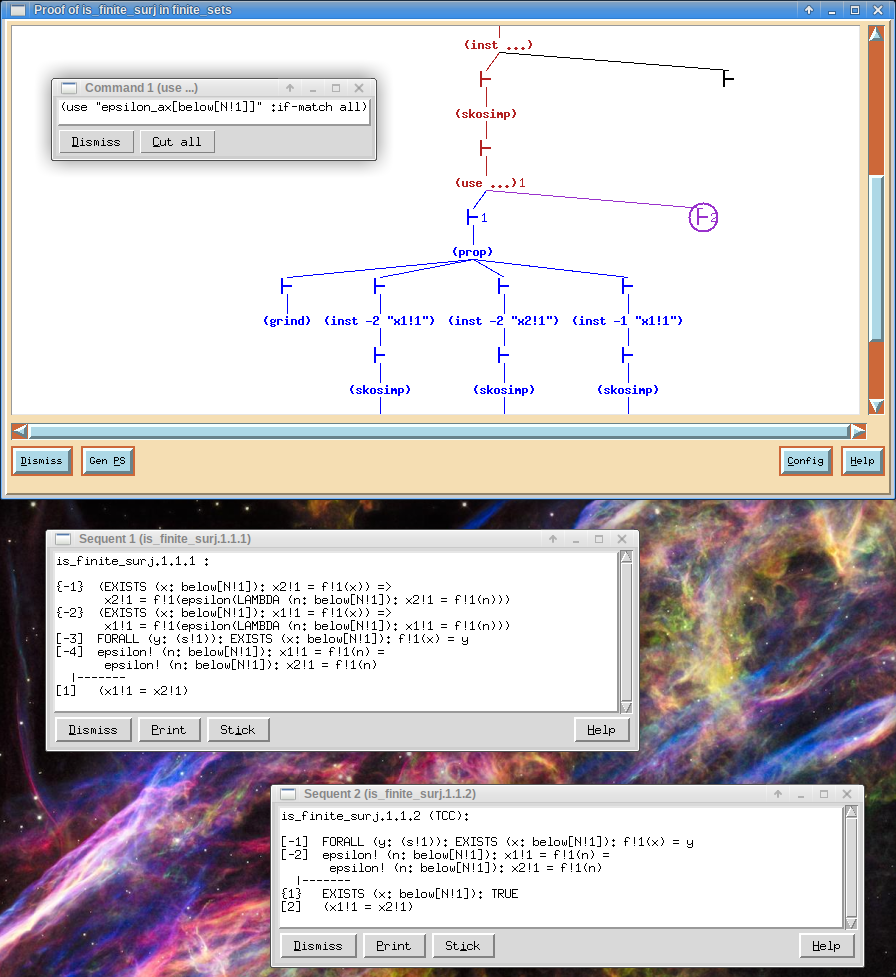
\includegraphics[width=\textwidth]{proofwindows.png}  
\caption{A Proof Display Example}\label{proofwindow}
\end{figure}

Colors are used to display status information about the proof.  These
colors may be specified using the X resource database (i.e., in your
\texttt{.Xresources} or \texttt{.Xdefaults} file).  Stipple patterns may
be specified instead of colors; a stipple pattern is specified as
\texttt{@file}, where \texttt{file} is either an absolute pathname of a
file in X bitmap format or the special bitmap name
\texttt{gray}.\footnote{If \texttt{file} is not an absolute path, it is
looked up in the \texttt{wish} subdirectory of the PVS directory, which
contains the \texttt{gray} bitmap.}

The current resources and their defaults are:

\begin{center}
\begin{tabular}{|lll|}\hline
  {\it Resource name} & {\it Color default} & {\it Monochrome default}%
     \\ \hline
  \texttt{pvs.windowbackground} & wheat & white \\
  \texttt{pvs.displaybackground} & white & white \\
  \texttt{pvs.displayforeground} & black & black \\
  \texttt{pvs.activedisplaybackground} & mediumslateblue & black \\
  \texttt{pvs.activedisplayforeground} & white & white \\
  \texttt{pvs.buttonbackground} & lightblue & white \\
  \texttt{pvs.buttonforeground} & black & black \\
  \texttt{pvs.activebuttonbackground} & steelblue & black \\
  \texttt{pvs.activebuttonforeground} & white & white \\
  \texttt{pvs.troughcolor} & sienna3 & black \\
  \texttt{pvs.currentColor} & DarkOrchid & black \\
  \texttt{pvs.circleCurrent} & yes & yes \\
  \texttt{pvs.tccColor} & green4 & black \\
  \texttt{pvs.doneColor} & blue & @gray \\
  \texttt{pvs.ancestorColor} & firebrick & black \\
  \texttt{pvs.abbrevLen} & 35 & 35 \\
  \texttt{pvs.displayfont} & \multicolumn{2}{l|}{lucidasanstypewriter-bold-12} \\
  \texttt{pvs.buttonfont} & \multicolumn{2}{l|}{lucidasanstypewriter-10} \\
  \texttt{pvs.proof.geometry} & \multicolumn{2}{l|}{\hspace*{.5in}\emph{none}} \\
  \texttt{pvs.theory-hierarchy.geometry} & \multicolumn{2}{l|}{\hspace*{.5in}\emph{none}} \\
  \texttt{pvs.prover-commands.geometry} & \multicolumn{2}{l|}{\hspace*{.5in}\emph{none}} \\
  \hline
\end{tabular}
\end{center}

The \texttt{foreground} color is used for things that aren't otherwise
specified below.  The \texttt{currentColor} is used for the current
sequent in the proof tree.  The \texttt{ancestorColor} is used for all
the ancestors of the current sequent, up to the root.  The
\texttt{doneColor} is used for sequents which have been proved.  The
\texttt{tccColor} is used for TCC's.  When \texttt{pvs.circle\-Current}
is set, the current sequent in the proof tree is circled.

Proof commands which are longer than \texttt{abbrevLen} characters are
abbreviated.

If the Emacs variable
\texttt{pvs-x-show-proofs}\index{pvs-x-show-proofs@\texttt{pvs-x-show-proofs}}
is not \texttt{NIL}, then \cmd{prove} automatically calls
\cmd{x-show-proof}.  This can be set in your
\texttt{.pvsemacs}\index{.pvsemacs@\texttt{.pvsemacs}} file.

The \cmd{x-theory-hierarchy} command prompts for a theory name and
displays the \texttt{IM\-PORTING} hierarchy rooted at that theory.  In a
complex hierarchy, it can be difficult to follow the lines; to make
this easier, when you move the mouse onto a theory identifier, all the
lines connecting that theory to other theories turn the
\texttt{highlight} color.  Clicking on a theory identifier will bring
up the theory in Emacs.  Figure~\ref{x-hierarchy} shows an example of the
theory hierarchy for the \texttt{finite\_sets} library, as produced from
clicking on the \texttt{Gen PS} button and selecting \texttt{portrait}.

\begin{figure}
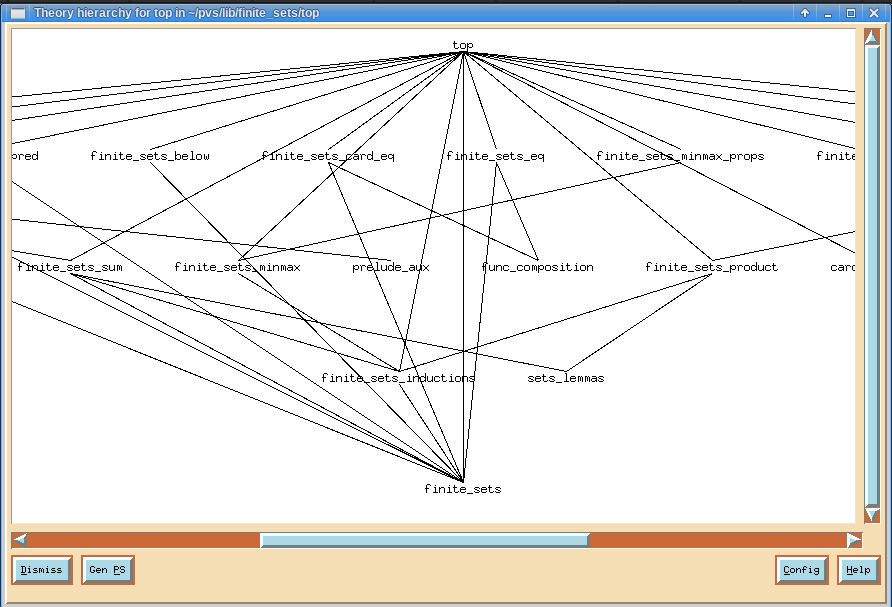
\includegraphics[width=\textwidth]{finite_sets_top_hier.png}
\caption{The Theory Hierarchy for the \texttt{finite\_sets} Library}\label{x-hierarchy}
\end{figure}


The remainder of this section applies to both \cmd{x-show-proof} and
\cmd{x-theory-hierarchy}.

The layout in the windows created by these commands can be manually
edited.  The editing commands are accessed by holding down the
\texttt{Control} key while pressing mouse buttons. In a proof window,
pressing \texttt{Control}-button~1 and dragging moves a whole proof
subtree, while \texttt{Control}-button~2 moves a single sequent.  In a
theory hierarchy window, \texttt{Control}-button~1 moves a theory.
(Note that most proof commands will do a relayout.)  Once the layout
is to your liking, the \texttt{Gen~PS} button will generate a
PostScript file which contains the contents of the window.  The
filename will be briefly displayed below the buttons.

The \texttt{Config} button will bring up a menu which will let you
customize the horizontal and vertical separations used by the
automatic layout for the current window.  These can also be customized
with the resource database.

\begin{center}
\begin{tabular}{|ll|}\hline
  {\it Resource name} & {\it Default} \\ \hline
  \texttt{pvs*proof*xSep} & 10 \\
  \texttt{pvs*proof*ySep} & 20 \\
  \texttt{pvs*th-hier*xSep} & 50 \\
  \texttt{pvs*th-hier*ySep} & 100 \\
  \hline
\end{tabular}
\end{center}


\section{Context Commands}

\begin{pvscmds}
\icmd{list-pvs-files} & \icmd{lf} & Display a list of PVS files in current context \\
\icmd{list-theories} & \icmd{lt} & Display a list of theories in current context \\
\icmd{change-context} & \icmd{cc} & Switch to a new context \\
\icmd{save-context} & \icmd{sc} & Save the current context \\
\icmd{pvs-remove-bin-files} & & Remove the \texttt{.bin} files of the current
context \\
\icmd{pvs-dont-write-bin-files} & & Inhibit writing or loading of
\texttt{.bin} files \\ 
\icmd{pvs-do-write-bin-files} & & Allows writing and loading of
\texttt{.bin} files (default) \\
\icmd{context-path} & \icmd{cp} & Display pathname of current context \\
\end{pvscmds}

The \cmd{list-pvs-files} and \cmd{list-theories} commands prompt for a
directory, default is to the current directory; if there is a PVS
context in the given directory, these commands list the PVS files or
theories in that context.  The resulting buffer is in a special mode,
which allows the file/theory to be viewed (by typing a ``\texttt{v}''),
selected (by typing a ``\texttt{s}'') or imported (by typing an ``{\tt
i}'').  A file or theory may only be selected if it is in the current
context, and may only be imported if it is not.  Importing a theory from
the list of theories will import the associated file.

The \cmd{change-context} command is similar to the ``\texttt{cd}'' command
in \unix; it saves the context (see below), and changes the working
directory to the specified one.  The \ibuf{PVS Welcome} buffer is then
displayed indicating the new directory.  If the requested directory does
not exist, and the Emacs you are running supports \texttt{make-directory},
then PVS offers to make a new one, including parent directories if necessary.
If the command fails for any reason, then the current context
stays the same.

The \cmd{save-context} command saves the current state of the session in
the context file \texttt{.pvscontext}.  In addition, any PVS files that
have been typechecked will generate a binary (\texttt{.bin}) file, unless
there is already a current one saved, or the \cmd{dont-write-bin-files}
command has been invoked.

Under normal circumstances, binary (\texttt{.bin}) files \index{.bin@\texttt{.bin}} corresponding to
the specification (\texttt{.pvs}) files are updated or created as needed.
These binary files contain type information, so that loading a binary file
has the same effect as typechecking the corresponding PVS file, but is
generally much faster.  The down side is that binary files take more disk
space.  If that is a problem then use the \cmd{pvs-dont-write-bin-files},
which neither loads nor creates binary files.  This can be added to your
\texttt{.pvsemacs}\index{.pvsemacs@\texttt{.pvsemacs}} file, by adding the
line
\begin{alltt}
  (pvs-dont-write-bin-files)
\end{alltt}
The \cmd{pvs-do-write-bin-files} undoes the effect of the
\cmd{pvs-dont-write-pvs-files}, and is not needed normally.  The
\cmd{pvs-remove-bin-files} command may be used to remove the binary files
that have been created.

The \cmd{context-path} command uses the minibuffer to display the
directory path associated with the current context.

\glossary{[directory path:] a file pathname containing sufficient
components to uniquely identify a directory}
\glossary{[context path:] a file pathname identifying the
directory which contains the context}

\section{Library Commands}

\begin{pvscmds}
\icmd{load-prelude-library} & & Extend the prelude from the specified context \\
\icmd{remove-prelude-library} & & Remove the specified context from the
prelude \\
\end{pvscmds}

The \cmd{load-prelude-library} command prompts for a context pathname
(\ie directory), and extends the prelude with all of the theories that
make up that context.  Note that the theories that make up the context are
defined by the \texttt{.pvscontext} file in the associated
directory---there may be specification files in the same directory that
are not a part of the context.  The files that make up the context are
typechecked if necessary, and internally the prelude is extended.  All of
the theories of the current context are untypechecked, as they may not
typecheck the same way in the extended prelude.  The PVS context is
updated to reflect that the prelude has been extended.  Thus the next time
this context is entered, the prelude will automatically be extended (by
typechecking the libraries if necessary).

This is just one of two means of gaining access to theories of a different
context (short of copying them).  For an alternative approach see the
language guide~\cite{PVS:language}.

The \cmd{remove-prelude-library} command removes the specified library
from the prelude.  It reverts all the theories of the current context to
untypechecked to guarantee that no theories depend on the removed library.
Note that the built-in prelude may not be removed this way.

\section{Browsing}

\begin{pvscmds}
\icmd{show-declaration} & \key{M-.} & Show declaration of symbol at cursor
\\
\icmd{goto-declaration} & \key{M-'} & Go to declaration of symbol at cursor \\
\icmd{find-declaration} & \key{M-,} & Search for declarations of given symbol \\
\icmd{whereis-declaration-used} & \key{M-;} & Search for declarations which reference identifier \\
\icmd{whereis-identifier-used} & \key{C-M-;} & Search for declarations which reference identifier \\
\icmd{list-declarations} & \key{M-:} & Produce list of declarations in import chain \\
\icmd{show-expanded-form} & \key{C-.} & Show expanded form of term
containing region\\
& & \emph{Arg:} also expand names from the prelude \\
\end{pvscmds}

These commands browse a specification consisting of several PVS files
and theories, providing information about where entities are declared
and used.  All of these commands browse the prelude as well as user
files.

The \cmd{show-declaration} command is used to determine the declaration
associated with the symbol or name at the cursor.  Positioning the cursor
on a name in the specification and typing \key{M-.} yields a pop-up
buffer displaying the declaration.  This command is useful to determine
the type of a name, or the resolution determined by the typechecker for an
overloaded name.  Note that when used on a record accessor it will
display the declaration of the record rather than just the record field.

The \cmd{goto-declaration} command goes to the declaration associated with
the symbol or name at the cursor.  It pops up a buffer containing the
theory associated with the declaration, and positions the cursor at the
declaration.

The \cmd{find-declaration} command takes a name and returns a list of all
the declarations with that name, the default name is the one under the
cursor. Each row in the display specifies the declaration name, its
kind/type, and the theory to which it belongs.  Declarations in this list
may be viewed by placing the cursor on the row of interest and typing
``\texttt{v}.''  Typing ``\texttt{s}'' will read in the associated file
and position the cursor at the declaration.  A ``\texttt{q}'' quits and
removes the declaration buffer.

The \cmd{whereis-declaration-used} command generates a list of
declarations which reference the entity denoted by a given identifier.
The related \cmd{whereis\-identifier-used} command generates a list of all
references to a \emph{textually identical} identifier, which may or may
not result from the same declaration, due to overloading and multiple
declarations.  The \cmd{list-declarations} command generates a listing of
all the declarations in the import chain of the specified theory.  For all
of these commands, the resulting buffer behaves exactly as described for
\icmd{find-declaration}.

The \cmd{show-expanded-form} command displays the expanded form of the
term containing the region in the \texttt{Expanded Form} buffer.  Each
variable, constant and operator is expanded to its full name including the
theory name and its parameters, unless they are from the current theory or
the prelude.  With an argument, prelude names are also expanded.  If the
region is not defined, the current cursor location is used instead.

%\memo{How about a \LaTeX\ version?}

\section{Theory Status}

\begin{pvscmds}
\icmd{status-theory} & \icmd{stt}, \key{C-c C-s t} & Status of specified theory (parsed, etc.) \\
\icmd{status-pvs-file} & \icmd{stf}, \key{C-c C-s f} & Status of theories of current file \\
\icmd{status-importchain} & \icmd{sti}, \key{C-c C-s i}  & Status of theories in import chain of theory \\
\icmd{status-importbychain} & \icmd{stb}, \key{C-c C-s b} & Status of
theories in import by chain \\
\end{pvscmds}

These commands provide information regarding the status of the
specified theories.  The status information for a theory indicates whether
it is parsed or typechecked, and provides the number of formulas, the
number proved, the number of TCCs generated, and the number of TCCs
proved.  Note that the number of formulas does not include the TCCs.

The number of theory warnings and messages is also displayed.  See the
\cmd{show-theory-warnings} and \cmd{show-theory-messages} on
page~\pageref{tc-info} for more information on these commands.

The \cmd{status-theory} command provides the status of the specified
theory in the mini\-buffer.  The \cmd{status-pvs-file},
\cmd{status-importchain}, and \cmd{status\-importbychain} commands display
the information in the \ibuf{PVS Status} buffer with a line for each
theory.  Using any of these commands on the \texttt{sum} theory yields
{\small
\begin{alltt}
sum is typechecked: 1 formula, 1 proved; 2 TCCs, 2 proved; 0 warnings; 0 msgs
\end{alltt}}
The \cmd{show-theory-warnings} and \cmd{show-theory-messages}
(page~\pageref{tc-info}) may be used to see any warnings or messages.

The \cmd{status-importchain} and \cmd{status-importbychain} commands
display the \texttt{IM\-PORT\-ING} chains of the specified theory, indented to
indicate the tree structure.  The \cmd{status-importchain} command works
recursively down the \texttt{IMPORTING}s, displaying the status of each
theory unless it has been displayed earlier in the buffer.  The
\cmd{status-importbychain} works in the opposite direction.


\section{Proof Status}
\label{proof-status}

\begin{pvscmds}
\icmd{status-proof} & \icmd{sp}, \key{C-c C-s p} & Status of formula at cursor \\
\icmd{status-proof-theory} & \icmd{spt} & Status of formulas in theory \\
 & & \emph{Arg:} provide timing information \\
\icmd{status-proof-pvs-file} & \icmd{spf} & Status of formulas in PVS file \\
 & & \emph{Arg:} provide timing information \\
\icmd{status-proof-importchain} & \icmd{spi} & Status of formulas on importchain \\
 & & \emph{Arg:} provide timing information \\
\icmd{status-proofchain} & \icmd{spc} & Proofchain of formula at cursor \\
\icmd{status-proofchain-theory} & \icmd{spct} & Proofchain of
specified theory \\
\icmd{status-proofchain-pvs-file} & \icmd{spcf} & Proofchain of current file \\
\icmd{status-proofchain-importchain} & \icmd{spci} & Proofchain of importchain \\
\end{pvscmds}

These commands provide the status of the proofs of the indicated formulas.
The \cmd{status-proof} command uses the minibuffer to display the proof
status of the formula at the cursor.  The status can be one of
\texttt{proved}, \texttt{untried}, \texttt{unfinished}, or
\texttt{unchecked}.  Untried means that the proof has not yet been
attempted.  Unfinished means that the proof has been attempted,
but is not complete.  Unchecked means that the proof was successful at one
point, but that some changes have been made that may invalidate the proof.

The commands \cmd{status-proof-theory}, \cmd{status-proof-pvs-file}, and
\cmd{status\-proof-importchain} use the \ibuf{PVS Status} buffer
to display the proof status for all of the formulas within the theory, PVS
file, or the import chain respectively.  With an argument, these commands
display timing information as well.

The \cmd{status-proofchain} command provides a proof chain analysis of the
formula at the cursor and displays it in the \ibuf{PVS Status} buffer.
The proof chain analysis indicates whether the formula has been proved,
and analyses the formulas used in the proof to insure that the proof is
complete; lemmas used in the proof are proved and sound, \ie\ there are no
circularities (for example, using lemma $\mathcal{A}$ to prove
$\mathcal{B}$ and vice-versa).  Because judgements are used implicitly,
they may be included in the analysis even if they are not actually used.

The commands \cmd{status-proofchain-theory},
\icmd{status-proofchain-pvs-file}, and \newline
\icmd{status-proofchain-importchain} provide the proof chain analysis for
each formula of the theory, PVS file, and import chain of the specified
theory, respectively, in the \ibuf{PVS Status} buffer.

\section{Environment Commands}

\begin{pvscmds}
\icmd{whereis-pvs} & & Display the root PVS directory \\
\icmd{pvs-version} & & Display current version of PVS and underlying \lisp \\
\icmd{pvs-mode} & & Put current buffer in PVS mode \\
\icmd{pvs-log} & & Display the \ibuf{PVS Log} buffer \\
\icmd{status-display} & & Display the \ibuf{PVS Status} buffer \\
\icmd{pvs-status} & & Find out if PVS is busy \\
\icmd{pvs} & & Start the PVS process \\
\icmd{pvs-load-patches} & & Load new PVS patches \\
\end{pvscmds}

The \cmd{whereis-pvs} command is used to determine the directory where the
PVS system resides.  This is useful for finding the example specifications
and files that are part of the PVS distribution.

The \cmd{pvs-version} command displays the current version of PVS\@.

The \cmd{pvs-mode} command puts the current buffer in PVS mode.  This
command is not normally needed; buffers with a \ibuf{.pvs}
extension and buffers created by PVS are automatically put in the
proper mode.

Most of the messages that appear in the minibuffer are kept in the
\ibuf{PVS Log} buffer, stamped with the time.  The \cmd{pvs-log} command
simply pops up the \ibuf{PVS Log} buffer so that you may view it.

The \cmd{status-display} command simply displays the \ibuf{PVS Status}
buffer.  This is the buffer used for most of the status commands.

The \cmd{pvs} command is what is used to actually start PVS after the
Emacs files have all been loaded.  It is provided as a user command
because there are times when the PVS lisp subprocess has been killed and
you wish to start up that process while keeping the same Emacs session.

The \cmd{pvs-load-patches} command reloads the patches.  This is useful
when new patches have been installed, and you wish to load them without
exiting the system and starting up again.


\section{Interrupting PVS}

\begin{pvscmds}
\icmd{pvs-status} & & Find out if Lisp is busy \\
\icmd{pvs-interrupt-subjob} & \key{C-c C-c} & Interrupt PVS (lisp)
  process \\
\icmd{reset-pvs} & \key{C-z C-g} & Abort PVS and resynchronize \\
\end{pvscmds}

Many PVS commands run in the background, allowing other editing
activities to proceed concurrently.  The effect of issuing new commands
while another command is running depends on the command: 
background commands placed on the command queue.  Other (nonbackground
commands) interrupt the currently running command, execute, and return
control to the interrupted command.  The Emacs status line indicates
the abbreviation of the command that is currently running, if any, or {\tt
ready}.  The \cmd{pvs-status} command provides information
about both the currently running command and the command queue.

To interrupt PVS for any reason, the following procedure is recommended.
First, if the keyboard is not responding, type the built-in Emacs
command \cmd{keyboard-quit} (\key{C-g}); it may need to be struck a few
times before there is any response---usually a beep and \texttt{Quit}
appears in the minibuffer.  This command interrupts Emacs, but has no
effect on any PVS commands that are still running.  After Emacs responds
go to the end of the \texttt{*pvs*} buffer, and type \key{C-c C-c}.  If
Lisp is able to respond, you should see the message
{\small\small
\begin{alltt}
Error: Received signal number 2 (Keyboard interrupt)
  [condition type: INTERRUPT-SIGNAL]

Restart actions (select using :continue):
 0: continue computation
 1: Return to Top Level (an "abort" restart)
[1c] PVS(22):
\end{alltt}}
You can then type \texttt{:continue 0} to keep going as it was never
interrupted, \texttt{(restore)} if you are in the middle of an ongoing
proof and want to continue from the state prior to the last \emph{atomic}
prover command (see the prover guide~\cite{PVS:prover}), or
\texttt{:continue 1} or \texttt{:reset} to abort to the top level.

The Lisp process may not be able to respond to the interrupt right away,
especially if it has started garbage collection.  If you really want to
interrupt it, type more \key{C-c C-c} interrupts; after about six of them
it is supposed to respond regardless.  This is not recommended in general
as it can leave the Lisp process in an unstable state.  Unfortunately, we
have seen Allegro Common Lisp get into a state where it is completely
unresponsive, even after several interrupts and waiting for hours for a
response.  This is rare, but if it happens the only recourse is to kill
the process and start up a new PVS session.  See below for how to do this
while allowing Emacs to continue.

The \cmd{reset-pvs} command aborts any ongoing activity in PVS; its
effects depend on whether it is issued from the \ibuf{*pvs*} buffer or
from some other buffer.  In the former case, \cmd{reset-pvs} simply
interrupts PVS as if you typed \key{C-c C-c}, as described above.  If
\cmd{reset-pvs} is issued somewhere other than the \ibuf{*pvs*} buffer,
you are asked whether to reset PVS in case the command was typed
accidentally; if not, the current command is aborted and the command queue
is emptied.

If you wish to kill the PVS Lisp process, while keeping your current Emacs
session, simply go to the \texttt{*pvs*} buffer and kill it
\icmd{kill-buffer} \key{C-x k}, then run \icmd{pvs} and the PVS Lisp
process will restart.  All your other Emacs buffers are unaffected by
this.

\setcounter{footnote}{0}
% Document Type: LaTeX
% Master File: user-guide.tex
\chapter{Customizing PVS}
\label{customization}
\index{customization}\index{PVS customization}

PVS is a complex system, and utilizes many subsystems, including Lisp,
Emacs, the X window system, and Tcl/Tk.  You can control aspects of these
subsystems by a combination of command-line arguments, environment
variables, and various files.  In this section we discuss some aspects of
the customization of these subsystems as they relate to PVS.

\section{Invoking PVS}\label{invoking-pvs}
\index{invoking PVS}\index{starting PVS}

PVS is invoked from a shell script named \texttt{pvs}\index{PVS shell
script} in the PVS directory---this is a text file, and may be examined or
copied and modified to suit your taste.  The script is a Bourne shell
script, and requires {\tt /bin/sh} to execute correctly.\footnote{On some
systems, \texttt{/bin/sh} is linked to the \texttt{bash} shell; this works
as well.}

PVS accepts a number of command-line arguments\index{PVS!command-line
arguments}\index{command-line arguments}, as well as using environment
variables.  The command-line arguments specific to PVS are
\begin{description}

\item[\texttt{-h | -help | --help}]\index{-help@\texttt{-help} command
line argument} - Print a brief description of the command line options and
exit.

\item[\texttt{-lisp} \emph{lispname}]\index{-lisp@\texttt{-lisp} command
line argument} - Specifies which lisp to use. The lisp image used for PVS
is then \texttt{pvs-\emph{lispname}}, which should be located in a
directory determined by the machine architecture.  See
Section~\ref{pvsimage}, page~\pageref{pvsimage} for details.

\label{dash-redhat}
\item[\texttt{-redhat}
\emph{redhat-release}]\index{-redhat@\texttt{-redhat} command line
argument} - Specifies the release of the Redhat Linux operating system you
are using (different PVS binaries are required for libc5 and glibc C
libraries).  PVS attempts to discover this for itself, but if the wrong
binary is chosen you can specify \texttt{4} or \texttt{5} using this
argument.  Note that Redhat 6 uses the glibc libraries, which corresponds
to the value \texttt{5}.

\item[\texttt{-runtime}]\index{-runtime@\texttt{-runtime} command line
argument} - This is only needed at SRI, where the development version of
the system is used by default.  With this option the runtime image is used
instead.

\item[\texttt{-emacs} \emph{emacsname}]\index{-emacs@\texttt{-emacs}
command line argument} - Specifies the Emacs to use; see below for
details.

\item[\texttt{-decision-procedures}
\emph{new}\texttt{|}\emph{old}]\index{-decision-procedures@\texttt{-decision-procedures}
command line argument} - Sets the default decision procedures to be used
in proofs.  See Section~\ref{decision-procedure-commands},
page~\pageref{decision-procedure-commands} for details.

\item[\texttt{-force-decision-procedures}
\emph{new}\texttt{|}\emph{old}]\index{-force-decision-procedures@\texttt{-force-decision-procedures}
command line argument} - Forces the chosen decision procedure to be used
regardless of the default decision procedure setting or which decision
procedures were used in developing a proof.  Note that with this option
there is no way to switch between the new and old decision procedures.

\item[\texttt{-nw}]\index{-nw@\texttt{-nw} command line argument} - Tells
Emacs not to use its special interface to X.

\item[\texttt{-batch}]\index{-batch@\texttt{-batch} command line argument}
- Run PVS in batch mode. See chapter~\ref{batchmode},
page~\pageref{batchmode} for details.

\item[\texttt{-timeout}:]\index{-timeout@\texttt{-timeout} command line
argument} In batch mode, this causes typechecking and individual proof
attempts to be interrupted after the given number of seconds.

\item[\texttt{-nobg}:]\index{-nobg@\texttt{-nobg} command line argument}
Normally PVS starts in the background (with the \& control operator).
This starts it in the foreground.

\item[\texttt{-raw}:]\index{-raw@\texttt{-raw} command line argument} This
runs PVS without Emacs.  This is only useful for front ends, which must do
the same initialization as done by the Emacs interface.

\item[\texttt{-v} \emph{number}]\index{-v@\texttt{-v} command line
argument} - Specifies verbosity level for PVS batch mode. See
Chapter~\ref{batchmode}, page~\pageref{batchmode} for details.

\label{dash-q-option}
\item[\texttt{-q}]\index{-q@\texttt{-q} command line argument} - A
standard emacs option to inhibit loading of the users {\tt .emacs} file,
but extended in PVS to inhibit loading of the users {\tt .pvsemacs}, {\tt
.pvsxemacs-options} and \texttt{.pvs.lisp} files on startup.

\item[\texttt{-patchlevel}
\emph{level}]\index{-patchlevel@\texttt{-patchlevel} command line
argument} - Specifies which patch files to load. Level \texttt{none} loads
no patch files. Level \texttt{rel} loads the file \texttt{patch2} from
your PVS directory, which usually contains the release versions of PVS
patches. Other valid levels are \texttt{test} (loads the files
\texttt{patch2} and \texttt{patch2-test}) and \texttt{exp} (loads the
files \texttt{patch2}, \texttt{patch2-test} and \texttt{patch2-exp}).
This option is mainly used for PVS development.


\end{description}
Any other command-line arguments are passed directly to the underlying
Emacs, including those for X windows---these are discussed
below.

In addition, the PVS script uses the environment
variables\index{PVS!environment variables}\index{environment variables}
\texttt{PVSLISP}\index{pvslisp@\texttt{PVSLISP}}\index{environment
variables!pvslisp@\texttt{PVSLISP}},
\texttt{PVSEMACS}\index{pvsemacs@\texttt{PVSEMACS}}\index{environment
variables!pvsemacs@\texttt{PVSEMACS}}, and
\texttt{PVSXINIT}\index{pvsxinit@\texttt{PVSXINIT}}\index{environment
variables!pvsxinit@\texttt{PVSXINIT}}, which may be set in your
\texttt{.cshrc} or \texttt{.login} file to specify the defaults you
prefer.  If both the environment variable and the corresponding
command-line argument are given, the command-line argument takes
precedence.  The \texttt{PVSXINIT} variable is described in
Section~\ref{windows}, page~\pageref{windows}.


\section{Emacs}
\index{Emacs|(}

The PVS system uses Emacs as its user interface, and provides a number of
files that extend Emacs for use with PVS.  For historical reasons, there
are currently a number of Emacs editors available.  Because we wanted PVS
to be freely available, we have chosen to concentrate on just \gnuemacs\
and XEmacs, which are also freely available.  To find out what version of
Emacs you are using, start up Emacs and type \iecmd{emacs-version}.  We
try to keep up with new releases of emacs and if necessary patch files
will be made available to support the new Emacs.

By default, the system uses \texttt{emacs}, which is assumed to be in your
path when you start up PVS.  You may specify a different Emacs as
specified above.  When you start PVS, is assumed (in order to supply X
resources in the correct format) that if the name of the emacs command
contains the character ``\texttt{x}'' then you are using XEmacs.

PVS loads your \texttt{\char'176/.emacs}\index{.emacs@\texttt{.emacs}}
file first (assuming you have not specified the {\tt -q} option as
described on page \pageref{dash-q-option}), followed by
\emph{PVSPATH}\texttt{/emacs/go-pvs.el}%
\index{go-pvs.el@\texttt{go-pvs.el}}, which determines which version of
emacs you are running and then loads the rest of the PVS emacs files,
including ILISP\index{ILISP}.  At this point you may receive an error from
PVS saying that your Emacs version is unknown.  PVS does not support Emacs
18 (or earlier), but we try to keep up with new Emacs versions as they are released.
Finally, the
\texttt{\char'176/.pvsemacs}\index{.pvsemacs@\texttt{.pvsemacs}} is
loaded.  If you are running XEmacs, the {\tt .pvsemacs} file will load
XEmacs options from the {\tt .pvsxemacs-options} file instead of the
standard {\tt .xemacs-options} file, as some are incompatible with
standard XEmacs.

In loading the files in this order, PVS functions and key
bindings will overwrite any conflicting ones defined in your
\texttt{.emacs} file.  \texttt{.pvsemacs} is the file to use to override
the key bindings and definitions given by PVS.  This approach was taken to
ensure that the behavior of PVS by default follows the user guide, but can
be readily modified to suit your taste.

One file that is worth noting is the
\emph{PVSPATH}\url{/emacs/emacs-src/pvs-abbreviations.el}%
\index{pvs-abbreviations.el@\texttt{pvs-abbreviations.el}} file, where the
abbreviations for many of the PVS commands are given.  You may define your
own abbreviations for commands you use a lot that don't currently have
abbreviations, by adding the appropriate lines in your \texttt{.pvsemacs}
file.  For example, adding
\begin{alltt}
  (pvs-abbreviate 'show-tccs 'st)
\end{alltt}
will make \ecmd{st} an abbreviation for \ecmd{show-tccs} in addition to
those already defined.  Note that you cannot redefine a name which is
already in use.

If you would like to byte-compile your Emacs customizations, create a
separate file, byte-compile it, and load it from your \texttt{.pvsemacs}.
Generally the kinds of forms provided in a \texttt{.pvsemacs} file are
simply variable settings and minor function definitions, and are not worth
byte-compiling.  It is only worthwhile if a function is being (re)defined
that will be invoked noninteractively and frequently, for example, if you
want to modify the way the process filter works.

\index{Emacs|)}


\section{The PVS Image}
\label{pvsimage}\index{PVS!lisp image|(}

PVS currently runs under Allegro Common Lisp on a number of different
platforms.  PVS is provided as a Common Lisp image, meaning that it
includes both the Lisp runtime system and the PVS programs, so you do not
need to have Allegro installed on your system.

There is usually just one PVS image available at a given site, and if the
system is properly installed, nothing further needs to be done.  If more
than one image is available, and the default one is not the desired one,
then it can be specified using either command-line arguments or
environment variables.  Invoking PVS with
{\smaller
\begin{alltt}
  pvs -lisp lucid -image pvs-lucid-sun4
\end{alltt}}
\noindent will use the \texttt{pvs-lucid-sun4} image.  Note that \texttt{-lisp
lucid} must be specified, so that the Emacs interface can be set up
properly.  For linux, also see the {\tt -redhat} option on page
\pageref{dash-redhat}.

Alternatively, the environment variables \texttt{PVSLISP} and
\texttt{PVSIMAGE} may be set to get the same effect.  Note that
command-line arguments take precedence.

After the PVS lisp image has started, it loads in the patch files as
specified by the {\tt -patchlevel} argument and then loads the file
{\tt .pvs.lisp} from your home directory.  This file can be used to
provide lisp customizations on a per user basis and for overriding
definitions in the patch file.

\index{PVS!lisp image|)}


\section{Window Systems}
\label{windows}

PVS was built primarily for the X window system\index{X windows}, though
it can be run from a terminal interface.
When run under X windows with the 
supported versions of Emacs, the resource name\index{resource
name}\index{PVS!resource name} will be set to \texttt{PVS}, and the
window\index{window name}\index{PVS!window name} and icon names\index{icon
name}\index{PVS!icon name} will be set to \texttt{PVS@}\textit{host\/},
where \textit{host\/} is the host name of the system on which PVS was
invoked.  These may be modified by adding command-line arguments or
setting the \texttt{PVSXINIT}\index{pvsxinit@\texttt{PVSXINIT}}%
\index{environment variables!pvsxinit@\texttt{PVSXINIT}} environment
variable.

You may customize the title and icon names by defining the function
\texttt{pvs-title-string} in your \texttt{.pvsemacs} file taking no
arguments and returning a string to be used as the title.  This function
is invoked at startup, and whenever the context is changed.  For example,
the following provides the name of the pvs path, the patch level
(\texttt{N} for none, \texttt{R} for released, \texttt{T} for test, and
\texttt{E} for experimental), the hostname, and the last two components of
the current context.

{\smaller
\begin{alltt}
    (defun pvs-title-string ()
      (format "%s%s%s:%s/"
          (trailing-components pvs-path 1)
        (cond ((stringp (cadddr *pvs-version-information*)) "E")
              ((stringp (caddr *pvs-version-information*)) "T")
              ((stringp (cadr *pvs-version-information*)) "R")
              (t "N"))
        (let ((host (car (string-split ?. (getenv "HOSTNAME")))))
          (format "@%s" host))
        (trailing-components *pvs-current-directory* 2)))
\end{alltt}}
\noindent For example, this might generate \url{pvs2.3N@photon:lib/finite_sets/}.

It is difficult to get a single setting for all of the Emacs versions; the
following table gives the arguments needed to set the resource, window,
and icon names for the various versions.

\begin{center}
\begin{tabular}{|l|l|l|l|} \hline
Emacs & Resource & Window & Icon \\ \hline\hline
emacs19 & \texttt{-rn} & \multicolumn{2}{|c|}{\texttt{-name}}\\ \hline
emacs19.29 (and later, & \multicolumn{3}{|c|}{\texttt{-name}}\\ 
including emacs20) & \multicolumn{3}{|c|}{ }\\ \hline
xemacs & \texttt{-name} & \texttt{-wn} & \texttt{-in} \\ \hline
\end{tabular}
\end{center}
\par\noindent Note: in emacs19, if \texttt{-rn} is not given, then
\texttt{-name} is used for the resource name as well.  Emacs19.29 and
later will give an error if the \texttt{-rn} argument is given.

The window name is the name used in the title bar of the PVS window, the
icon name is the name used in the icon, and the resource name is the name
referred to in the \texttt{.Xdefault} or \texttt{.Xresource} file that
controls the defaults for X clients.  An example entry for PVS in one of
these files might be
\begin{alltt}
!	PVS defaults
PVS.geometry: 80x63-0-0
PVS*pointerColor: Red
PVS*Font: *courier-medium-r-normal--12*
\end{alltt}
See the man pages for \texttt{X} and \texttt{emacs}, as well as the news
and info pages for the version of Emacs you are using for more details on
X resources.

The \texttt{PVSXINIT} environment variable may be set\footnote{Generally
environment variables are set in your shell startup file, \emph{e.g.},
\texttt{.profile} or \texttt{.cshrc}.} to a string
of command-line arguments that are then appended to the defaults described
above.  You can also change the default resource, window, and icon names,
simply by adding them to this variable (or by including them in the
command-line arguments).  Note that you should make certain that the
version of Emacs you are using matches the command-line arguments as shown
in the footnote.  You can tell that there is a mismatch when you start up
PVS and find buffers with names matching command-line arguments, \eg\
\texttt{-in} or \texttt{PVS@acorn}.

\setcounter{footnote}{0}
% Document Type: LaTeX
% Master File: user-guide.tex
% Use latex2e to process this file
\chapter{Running PVS in Batch Mode}
\label{batchmode}

To support validation runs, PVS supports a \emph{batch mode}, which
means that specifications and proofs being processed are not displayed.
In batch mode there is no direct interaction with PVS; it simply processes
whatever files or functions are provided and terminates after completing
the last of them.  PVS batch mode is built directly on the underlying
Emacs batch mode described in Section A.2 of the GNU Emacs
Manual~\cite{emacs20}.

If PVS is invoked in batch mode from a shell, then it may be interrupted
(using \texttt{C-c}), suspended (\texttt{C-z}), or run as a background
job.  The output may be redirected to a file or piped to another
command.\footnote{The Emacs batch option actually sends its output to
\texttt{stderr} rather than \texttt{stdout}; the \texttt{pvs} shell script
redirects this to \texttt{stdout}, as this is generally more useful and
easier to work with.}

To run PVS in batch mode, simply include the `\texttt{-batch}' option in
your call to PVS.  In addition, you should include one or more Emacs
source files and/or a Emacs or PVS function to run, using the `\texttt{-l}' or
`\texttt{-load}' option to load a file, and the `\texttt{-f}' or
`\texttt{-funcall}' option for a function.  For example:
\begin{alltt}
  pvs -batch -l test.el
  pvs -batch -f pvs-version
\end{alltt}
Note that the function option is severely limited, as it only allows a
function name.  This means that only functions that take no arguments may
be provided, for example, \texttt{pvs-version} or \texttt{whereis-pvs}.

Running PVS in batch mode does cause your \texttt{\char'176/.emacs} file
to be loaded, in contrast to running Emacs in batch mode.  If you want
to suppress the loading of your \texttt{.emacs}, include the
`\texttt{-q}' option, for example:
\begin{alltt}
  pvs -batch -q -l test.el
\end{alltt}

In batch mode PVS suppresses messages by default, though you can print
your own messages.  You can also control the amount of printout using the
verbose option, `\texttt{-v}', and providing a level number ranging from
\texttt{0} to \texttt{3}.
The following table summarizes the levels.
\begin{center}
\begin{tabular}{|l|l|}\hline
\textbf{level} & \textbf{printout} \\ \hline
0 & User-defined \texttt{pvs-message}s only \\
1 & Messages normally sent to the echo area and PVS errors\\
2 & Status buffers \\
3 & Proof replays \\ \hline
\end{tabular}
\end{center}

The \texttt{pvs-message} function is much like the Emacs \texttt{message}
function, but the message will get printed no matter what the level number
is.  If you want to print out only when the level is \texttt{1} or higher,
use \texttt{message} instead.  Both take a control string and an arbitrary
number of arguments.  An example is shown in Figure~\ref{batch-file}.

The file provided to the load option (`\texttt{-l}' or `\texttt{-load}')
is an ordinary Emacs file, and usually has an \texttt{.el} extension.
Inside this file you can invoke any PVS commands you want, though many of
them only make sense interactively.  For example, the \texttt{prove}
command expects the cursor to be positioned at a given formula, which is
difficult (though not impossible) to do in batch mode.  The various Tcl/Tk
commands available will not run at all because there is no X display
associated with PVS running in batch mode.  The most useful commands to
run in batch mode are listed in Table~\ref{batch-commands}.  In that table, a
\textit{filename} is a PVS file name without the \texttt{.pvs} extension,
a \textit{theoryname} is the name of a theory in the current context, and
a \textit{directory} is a Unix pathname.  These must all be given as
strings (enclosed in double quotes).  The \textit{length} and
\textit{depth} arguments are integers, and do not need any special
treatment.  PVS Emacs commands are given in Emacs lisp syntax; for
example,
\begin{alltt}
  (parse "foo")
  (set-print-depth 3)
  (save-context)
\end{alltt}

\begin{table}
\begin{center}
\begin{tabular}{|l|l|}\hline
\textbf{Command} & \textbf{Arguments} \\ \hline
\texttt{parse} & \textit{filename} \\
\texttt{typecheck} & \textit{filename} \\
\texttt{typecheck-importchain} & \textit{filename} \\
\texttt{typecheck-prove} & \textit{filename} \\
\texttt{typecheck-prove-importchain} & \textit{filename} \\
\texttt{prove-theory} & \textit{theoryname} \\
\texttt{prove-pvs-file} & \textit{filename} \\
\texttt{prove-importchain} & \textit{theoryname} \\
\texttt{set-print-depth} & \textit{depth} \\
\texttt{set-print-length} & \textit{length} \\
\texttt{set-rewrite-depth} & \textit{depth} \\
\texttt{set-rewrite-length} & \textit{length} \\
\texttt{alltt-theory} & \textit{theoryname} \\
\texttt{alltt-pvs-file} & \textit{filename} \\
\texttt{alltt-importchain} & \textit{theoryname} \\
\texttt{latex-theory} & \textit{theoryname} \\
\texttt{latex-pvs-file} & \textit{filename} \\
\texttt{latex-importchain} & \textit{theoryname} \\
\texttt{latex-set-linelength} & \textit{length} \\
\texttt{change-context} & \textit{directory} \\
\texttt{save-context} & \\
\texttt{pvs-remove-bin-files} & \\
\texttt{pvs-dont-write-bin-files} & \\
\texttt{pvs-do-write-bin-files} & \\
\texttt{status-theory} & \textit{theoryname} \\
\texttt{status-pvs-file} & \textit{filename} \\
\texttt{status-importchain} & \textit{theoryname} \\
\texttt{status-importbychain} & \textit{theoryname} \\
\texttt{status-proof-theory} & \textit{theoryname} \\
\texttt{status-proof-pvs-file} & \textit{filename} \\
\texttt{status-proof-importchain} & \textit{theoryname} \\
\texttt{status-proofchain-theory} & \textit{theoryname} \\
\texttt{status-proofchain-pvs-file} & \textit{filename} \\
\hline
\end{tabular}
\end{center}
\caption{Commands available for validation}\label{batch-commands}
\end{table}

An example of the contents of a batch file is shown in
Figure~\ref{batch-file}.  This file consists of three commands.  It prints
the message ``\texttt{Proving stamps2}'', changes to the
\texttt{\char'176/pvs/test} context, and then reruns all the proofs of the
specification file \texttt{stamps2.pvs}.  Note that
\texttt{current-prefix-arg} is set to \texttt{t} to ensure that the proofs
are retried.  This is equivalent to using \texttt{C-u} interactively.
\begin{figure}
\begin{center}
\fboxsep=10pt%
\begin{boxedminipage}{3.2in}
\begin{alltt}
(pvs-message "Proving stamps2")
(change-context "~/pvs/test")
(let ((current-prefix-arg t))
  (prove-pvs-file "stamps2"))
\end{alltt}
\end{boxedminipage}
\end{center}
\caption{Batch File Example}\label{batch-file}
\end{figure}
While PVS is running in batch mode, two possible kinds of error may be
encountered.  An Emacs error comes from badly formed batch files or
nonexistent functions.  These errors will cause the system to stop
immediately, and the error will be displayed if the level number is
nonzero.  A PVS error generates an error message (for a nonzero level
number) and abandons the current command, but allows the system to go on
to the next command.

If an emacs error is encountered that reports 'entering debugger' when
run with verbosity level 3, the full commands of the emacs debugger
are available\footnote{See the Emacs manual\cite{emacs20} for details.}.
A useful command to discover where your validation script encountered the error is:
\begin{alltt}
e (progn (set-buffer "*Backtrace*")(buffer-string))
\end{alltt}

Another potential pitfall is that PVS may appear to hang.  If this
happens, try running with verbosity level 3 as it is likely that PVS
is awaiting user input (usually a yes/no).  You may respond to such
prompts from the shell. 

\section{Validation Runs}

A validation run is simply a batch run in which the \texttt{pvs-validate}
macro is used in the batch file.  Given a \emph{log file} name, a
directory, and a sequence of PVS Emacs commands, \texttt{pvs-validate}
will change context to the specified directory and run the commands,
collecting the output into the log file.  It then compares the new results
to the previous ones, and reports whether there were any significant
differences.  An example of the use of \texttt{pvs-validate} is shown in
Figure~\ref{validate-file}.
\begin{figure}
\begin{center}
\fboxsep=10pt%
\begin{boxedminipage}{3.3in}
\begin{alltt}
(pvs-validate
  "stamps2.log"
  "~/pvs/test"
  (pvs-message "Proving stamps2")
  (set-rewrite-depth 0)
  (let ((current-prefix-arg t))
    (prove-pvs-file "stamps2")))
\end{alltt}
\end{boxedminipage}
\end{center}
\caption{Example Use of \texttt{pvs-validate}}\label{validate-file}
\end{figure}

Any number of \texttt{pvs-validate} forms may be used, and they may be
freely intermixed with other Emacs or PVS commands.  When the sequence of
commands associated with an invocation of \texttt{pvs-validate} is
complete, the log file is compared to the previous version, if it exists.
At this point PVS will report one of three messages:
\begin{itemize}
\item \texttt{Nothing to compare \textit{log} to} - the log file has not
been generated before this run.

\item \texttt{No significant changes in \textit{log}} - the current run
does not differ significantly from the last one.  A significant difference
is one that involves more than timing differences.  For example, the
message \texttt{proved in 27 seconds} is not significantly different from
\texttt{proved in 31 seconds}.

\item \texttt{Differences found since last run} - differences were
found.  The following line indicates the two log files that should be
compared to see where they differ.
\end{itemize}

This is normally all the output provided by PVS while processing a
\texttt{pvs-validate} macro, though you can get more information by
including the `\texttt{-v}' option as described above.

With minor exceptions, the log files contain the same information as
obtained with the `\texttt{-v 3}' option, but only for the commands of the
given \texttt{pvs-validate} macro.  In comparing log files, timings are
ignored.\footnote{In the future we may want to compare timings and report
those that are significantly different, but in order for this to work
properly we must get CPU times rather than real times, and make sure that
we are keeping track of the machine used for the previous validation run
For now we are only concerned with functional correctness.}

When a difference is reported, you can find out what the differences
actually are by starting up (an interactive) PVS, and bringing up the two
files in a split window.\footnote{In detail, start up PVS, use \texttt{C-x
C-f} to visit the first file, use \texttt{C-x 2} to split the window
vertically, and then use \texttt{C-x C-f} again to bring in the second
file.}  Then use \texttt{M-x pvs-compare-validation-windows}, which works
much like the Emacs \texttt{compare-windows} command, and will position
the cursor at the point where the two files differ.  Again, differences in
timing are ignored.  After analyzing the difference, you can move the
pointer in each buffer to the next position where they are the same, and
run \texttt{M-x pvs-compare-validation-windows} again to get to the next
difference.  In this way you can quickly analyze all the differences since
the last validation run.

The log files are maintained under RCS~\cite{RCS}, using the Emacs
\emph{Version Control} interface~\cite{emacs20}.  The first time
a validation run is made from a given directory, an RCS subdirectory is
created to keep the directory from being cluttered with RCS files.
If this is the first validation run for a given log file, then the log
file is created and registered to RCS.  In subsequent runs, the log file
is compared to the previous version, which will have a name including the
version number, for example, \texttt{stamps2.log.\char'176 1.8\char'176}.
If the comparison shows no significant differences, then the file is
subsequently deleted.

Note that the log files are all kept in the directory from which PVS was
run, and changing context will not affect that.  This makes it easy to
maintain a single directory that controls the validation for several
different contexts.

\section{Example Validation Run}
Here is an example of a validation run for a very simple specification.
\subsection{The Specification}
The specification is in the file \texttt{stamps.pvs}:
\begin{alltt}
stamps : THEORY
 BEGIN
  i, n3, n5: VAR nat
  stamps: LEMMA (FORALL i: (EXISTS n3, n5: i+8 = 3*n3 + 5*n5))
 END stamps
\end{alltt}
\subsection{The Validation File} 
The file \texttt{stamps.el} has the validation commands.  In this case we
are simply going to reprove the formulas of the specification file (there
is only one):
\begin{alltt}
(pvs-validate
 "stamps.log"
 "~/pvs-specs/validation"
 (pvs-message "Proving stamps")
 (let ((current-prefix-arg t))
   (prove-pvs-file "stamps")))
\end{alltt}
\subsection{The Validation Run}
Here is the validation run, with level number 1.  This shows the messages
that normally appear in the echo area at the bottom of the Emacs window
(these messages are sent to \texttt{stdout}):
\begin{alltt}
% ./pvs -batch -l stamps.el -v 1
Started initializing ILISP
Finished initializing pvsallegro
Loading compiled patch file /project/pvs/patch2.fasl
Context changed to ~/pvs-specs/validation/
Checking out ~/pvs-specs/validation/stamps.log...
Checking out ~/pvs-specs/validation/stamps.log...done
PVS Version 2.3 (No patches loaded)
Context changed to ~/pvs-specs/validation/
Proving stamps
Parsing stamps
stamps parsed in 0.02 seconds
Typechecking stamps
stamps typechecked in 0.02s: No TCCs generated
Rerunning proof of stamps
Using old decision procedures
Proving stamps.stamps.
Proving stamps.stamps..
Proving stamps.stamps...
Proving stamps.stamps....
Proving stamps.stamps.....
Proving stamps.stamps......
Proving stamps.stamps.......
stamps proved in 2.20 real, 0.58 cpu seconds
stamps: 1 proofs attempted, 1 proved in 2.20 real, 0.58 cpu seconds
Checking out ~/pvs-specs/validation/stamps.log.~1.3~...
Checking out ~/pvs-specs/validation/stamps.log.~1.3~...done
No significant changes in stamps.log
Checking in ~/pvs-specs/validation/stamps.log...
Checking in ~/pvs-specs/validation/stamps.log...done
\end{alltt}

\subsection{The Log File}
The resulting log file \texttt{stamps.log} is shown here.  This will
be used for comparison to in subsequent validation runs.
{\small
\begin{alltt}
PVS Version 2.3 (No patches loaded)
Context changed to ~/pvs-specs/validation/
Proving stamps
Restoring theories from stamps.bin
Restored file stamps (stamps) in 0.57 seconds
Rerunning proof of stamps
Using old decision procedures

stamps :  

  |-------
\{1\}    (FORALL i: (EXISTS n3, n5: i + 8 = 3 * n3 + 5 * n5))

Proving stamps.stamps.
Rerunning step: (INDUCT "i")
Proving stamps.stamps..
Inducting on i,
this yields  2 subgoals: 
stamps.1 :  

  |-------
\{1\}    (EXISTS (n3: nat), (n5: nat): 0 + 8 = 3 * n3 + 5 * n5)

Rerunning step: (INST + 1 1)
Instantiating the top quantifier in + with the terms: 
 1, 1,
this simplifies to: 
stamps.1 :  

  |-------
\{1\}    0 + 8 = 3 * 1 + 5 * 1

Rerunning step: (ASSERT)
Simplifying, rewriting, and recording with decision procedures,

This completes the proof of stamps.1.

stamps.2 :  

  |-------
\{1\}    (FORALL (j: nat):
         (EXISTS (n3: nat), (n5: nat): j + 8 = 3 * n3 + 5 * n5)
             IMPLIES (EXISTS (n3: nat), (n5: nat):
                         j + 1 + 8 = 3 * n3 + 5 * n5))

Rerunning step: (SKOSIMP*)
Repeatedly Skolemizing and flattening,
this simplifies to: 
stamps.2 :  

\{-1\}    j!1 + 8 = 3 * n3!1 + 5 * n5!1
  |-------
\{1\}    (EXISTS (n3: nat), (n5: nat): j!1 + 1 + 8 = 3 * n3 + 5 * n5)

Rerunning step: (CASE "n5!1 = 0")
Case splitting on 
Proving stamps.stamps...
   n5!1 = 0, 
this yields  2 subgoals: 
stamps.2.1 :  

\{-1\}    n5!1 = 0
[-2]    j!1 + 8 = 3 * n3!1 + 5 * n5!1
  |-------
[1]    (EXISTS (n3: nat), (n5: nat): j!1 + 1 + 8 = 3 * n3 + 5 * n5)

Proving stamps.stamps....
Rerunning step: (INST + "n3!1 - 3" 2)
Instantiating the top quantifier in + with the terms: 
Proving stamps.stamps.....
 n3!1 - 3, 2,
this yields  2 subgoals: 
stamps.2.1.1 :  

[-1]    n5!1 = 0
[-2]    j!1 + 8 = 3 * n3!1 + 5 * n5!1
  |-------
\{1\}    j!1 + 1 + 8 = 3 * (n3!1 - 3) + 5 * 2

Rerunning step: (ASSERT)
Simplifying, rewriting, and recording with decision procedures,

This completes the proof of stamps.2.1.1.

stamps.2.1.2 (TCC):   

[-1]    n5!1 = 0
[-2]    j!1 + 8 = 3 * n3!1 + 5 * n5!1
  |-------
\{1\}    n3!1 - 3 >= 0

Rerunning step: (ASSERT)
Simplifying, rewriting, and recording with decision procedures,

This completes the proof of stamps.2.1.2.


This completes the proof of stamps.2.1.

stamps.2.2 :  

[-1]    j!1 + 8 = 3 * n3!1 + 5 * n5!1
  |-------
\{1\}    n5!1 = 0
[2]    (EXISTS (n3: nat), (n5: nat): j!1 + 1 + 8 = 3 * n3 + 5 * n5)

Proving stamps.stamps......
Rerunning step: (INST + "n3!1 + 2" "n5!1 - 1")
Instantiating the top quantifier in + with the terms: 
Proving stamps.stamps.......
 n3!1 + 2, n5!1 - 1,
this yields  2 subgoals: 
stamps.2.2.1 :  

[-1]    j!1 + 8 = 3 * n3!1 + 5 * n5!1
  |-------
[1]    n5!1 = 0
\{2\}    j!1 + 1 + 8 = 3 * (n3!1 + 2) + 5 * (n5!1 - 1)

Rerunning step: (ASSERT)
Simplifying, rewriting, and recording with decision procedures,

This completes the proof of stamps.2.2.1.

stamps.2.2.2 (TCC):   

[-1]    j!1 + 8 = 3 * n3!1 + 5 * n5!1
  |-------
\{1\}    n5!1 - 1 >= 0
[2]    n5!1 = 0

Rerunning step: (ASSERT)
Simplifying, rewriting, and recording with decision procedures,

This completes the proof of stamps.2.2.2.


This completes the proof of stamps.2.2.


This completes the proof of stamps.2.

Q.E.D.
stamps proved in 19 seconds
stamps: 1 proofs attempted, 1 proved in 19 seconds


 Proof summary for theory stamps
    stamps..........................................proved - complete
    Theory totals: 1 formulas, 1 attempted, 1 succeeded.

Grand Totals: 1 proofs, 1 attempted, 1 succeeded.
\end{alltt}}

%\include{ug-buffers}

%\pagebreak
%\def\glossaryentry#1#2{\item#1}
%%\newcommand{\glossaryentry}[2]{foo #1}
%\chapter{Glossary}

%% NB: \input{ug.glo} will not work; the file is empty because of
%% \makeglossary by the time it gets here.  Instead, copy ug.glo to
%% ug.gls
%\begin{description}
%\input{ug.gls}
%\end{description}

\pagebreak
\appendix
%\chapter{The Grammar}\label{grammar}

The complete \pvs\ grammar is presented in this Appendix, along with a
discussion of the notation used in presenting the grammar.

The conventions used in the presentation of the syntax are as follows.
\index{syntax!conventions}

\begin{itemize}

\item Names in {\it italics\/} indicate syntactic classes and
metavariables ranging over syntactic classes.

\item The reserved words of the language are
      printed in \lit{tt font, UPPERCASE}.

\item An optional part {\it A\/} of a clause is enclosed in square brackets:
\opt{{\it A\/}}.

\item Alternatives in a syntax production are separated by a bar
(``\choice''); a list of alternatives that is embedded in the right-hand
side of a syntax production is enclosed in brackets, as in

\begin{bnf}
\production{ExportingName}
{IdOp \opt{\lit{:} \brc{TypeExpr \choice \lit{TYPE} \choice \lit{FORMULA}}}}
\end{bnf}


\item Iteration of a clause {\it B\/} one or more times is indicated by
enclosing it in brackets followed by a plus sign: \ite{{\it B\/}};
repetition zero or more times is indicated by an asterisk instead of the
plus sign: \rep{{\it B\/}}.

\item A double plus or double asterisk indicates a clause separator; for
example, \reps{{\it B\/}}{,} indicates zero or more repetitions of the
clause {\it B} separated by commas.

\item Other items printed in tt font on the right hand side of
      productions are literals.  Be careful to distinguish where BNF
symbols occur as literals, \eg\ the BNF brackets \brc{} versus the
literal brackets \lit{\{\}}.

\end{itemize}

\subsubsection*{Specification}
\par\noindent
\spvsbnf{bnf-theory}

\subsubsection*{Importings and Exportings}
\par\noindent
\spvsbnf{bnf-exporting}

\subsubsection*{Assumings}
\par\noindent
\spvsbnf{bnf-assuming}

\subsubsection*{Theory Part}
\par\noindent
\spvsbnf{bnf-theory-part}

\subsubsection*{Declarations}
\par\noindent
\spvsbnf{bnf-decls}

\subsubsection*{Type Expressions}
\par\noindent
\spvsbnf{bnf-type-expr}

\subsubsection*{Expressions}
\par\noindent
\spvsbnf{bnf-expr}

\subsubsection*{Expressions (continued)}
\par\noindent
\spvsbnf{bnf-expr-aux}

\subsubsection*{Names}
\par\noindent
\spvsbnf{bnf-names}

\subsubsection*{Identifiers}
\par\noindent
\spvsbnf{bnf-lexical}

\subsubsection*{Datatypes}
\par\noindent
\spvsbnf{bnf-adts}

%\setcounter{footnote}{0}
%\input{whats-new}
%\setcounter{footnote}{0}
% \input{ug-install}
% \pagebreak
%\setcounter{footnote}{0}
%\input{trouble}
%\pagebreak
\setcounter{footnote}{0}
% Document Type: LaTeX
% Master File: user-guide.tex
\chapter{Introduction to Emacs}
\label{emacs-intro}

The PVS system uses the GNU Emacs system as its user interface.  To make
effective use of PVS, you must become familiar with at least the basic
Emacs commands.  This section provides an introduction to Emacs that
should allow you to get started in PVS right away.  This Appendix
introduces enough of the basic ideas and commands of Emacs to use PVS, but
to become effective you really should consult the GNU Emacs
Manual~\cite{emacs20}.  It is also quite helpful to run through the online
tutorial.  To do this, start up PVS or Emacs, type \key{C-h t}, and follow
the instructions.

Emacs provides the primary interface to the PVS system.  We chose Emacs
as our interface for a number of reasons.  First, it is freely available,
and runs on a large number of different platforms.  It is also quite
popular; on Unix systems the \texttt{vi} editor is probably the only
editor that is used more than Emacs, but it is too limited to use as a
general-purpose interface.  In particular, it has no support for running
subprocesses.

Emacs is an extremely flexible editor, and includes a built in programming
language (Emacs Lisp) which makes it easy to increase its functionality.
There is a cost associated with this.  First, Emacs is rather large, and
takes longer to start up than smaller editors such as \texttt{vi}.  Emacs
is also quite complex, with a large number of commands and associated key
bindings that are not easy to learn.

Emacs is significantly different than other editors.  In most editors, you
start the editor, get a file, make some changes, save the file, and exit.
There is a tendency to think in terms of ``leaving'' the current file in
order to go to the next. To handle multiple files in a single session
usually requires extra care and some specialized commands.  For example,
\texttt{vi} can only focus on one file at a time, with one alternate.

In Emacs multiple buffers may be open at once, and as many can be made
visible as your screen allows.  Unlike other editors, buffers are not all
associated with files.  It is not unusual to have over a hundred buffers
associated with a single Emacs session.  It is also quite normal to have
the same Emacs session up for weeks at a time.\footnote{Some people have
even been known to use Emacs as their shell.}  When you are done editing
and saving a given file, you do not exit from that buffer, you simply go
on to the next one.

Unlike \texttt{vi}, there is no command mode.  By default an Emacs buffer
is in insert mode, and most keys on the keyboard simply insert themselves.
Emacs has a large number of interactive commands, any of which may be
bound to a key or key sequence.\footnote{It turns out that typing a letter
key actually invokes the command \texttt{self-insert-command}.}  Any
interactive command may be invoked by typing \texttt{M-x} followed by the
command.  Recall that \texttt{M-x} is gotten by holding down the
\texttt{Meta-} key and typing an \texttt{x}.  If you don't have a key
labeled \texttt{Meta-}, then look for and try the \texttt{Alt} or
$\Diamond$ keys.  If you really don't have a \texttt{Meta-} key, then the
\texttt{Esc} key will do, but in this case you must release the
\texttt{Esc} key before typing the \texttt{x}.

Commands may be bound to key sequences, in order to make typing easier.
For example, to page down repeatedly by typing \texttt{M-x
scroll-up} over and over would get quite tedious, so the key sequence
\texttt{C-v} was bound to this command.  This and most of the key bindings
of Emacs are not particularly mnemonic, but once learned they are
extremely effective.  With a little practice you will find that you don't
think about what key sequence is needed to get a particular effect---your
hands just do it automatically.

Each buffer in Emacs has an associated major mode, and any number of minor
modes.  The major mode indicates what kind of a buffer it is, and
generally defines the key bindings and functions associated with the
buffer.  This is usually determined from the file extension, so for
example the file \texttt{foo.pvs} is in \texttt{pvs-mode}, while a file
\texttt{foo.c} would normally be in \texttt{c-mode}.  Minor modes modify
the major mode.  Examples include \texttt{auto-fill-mode} and
\texttt{overwrite-mode}.

When you start up PVS, you will see the \texttt{PVS Welcome} buffer, which
takes up most of the window.  Toward the bottom of the window you will see
a line in inverse video; this is the mode line.  The last line of the
window is the minibuffer.  If you are running Emacs version 19 (or later) under X
windows, then you will see a menu line at the top of the window, and a
scroll bar to the right.  If you display more than one buffer in the
window, then the bottom of each buffer will have a mode line displaying
information for that buffer.  There will still be only one minibuffer,
however.\footnote{In Emacs 19 (and later versions), it is possible to have multiple windows,
called frames, associated with a single Emacs session.  In this case, each
frame by default has its own copy of the minibuffer.  See the Emacs manual
for more details.}

The mode line provides information relating to the buffer above it.  The
first five characters indicate whether the buffer is read-only, and
whether the buffer has changed relative to the file.  If you see
\texttt{---\%\%-}, then the file is read-only, and you will not be allowed
to modify it.  Sometimes this is set when you have copied a file from
somewhere else, and you think you should be able to make modifications.
In that case, use the \texttt{toggle-read-only} command, make your
changes, and save the file.  Emacs may still ask whether it should try to
save the file anyway, go ahead and answer yes in this case.

If the mode line is 5 dashes (\texttt{-----}), then the file can be
modified but has not yet been changed.  Once modified, the mode line
changes to \texttt{--**-}.  If you did not intend to modify the file, then
use the \texttt{undo} commands described below to undo your change.  If there are a
few changes, you may need to repeat the \texttt{undo} command until they
are all backed out.  If there are a lot of changes, then \texttt{M-x
revert-buffer} may be used to restore the buffer from the original file.
The other information in the mode line is the buffer name, possibly the
time, the mode of the buffer in parentheses, and the amount of the buffer
currently displayed.  Like everything else in Emacs, the mode line is
customizable; see the Emacs manual for details.

The minibuffer is used to display messages, echo longer commands as they
are typed in, and prompt for arguments.  Many of these arguments support
\emph{completion}, which means that you can type the start of an argument
and type a \texttt{TAB} to have it automatically filled in.  Emacs will
fill in as much as is unique, and then wait for more input.  If it is
ambiguous already, Emacs will pop up a buffer with the possible
completions in it.  You can force it to show all possible completions by
typing a \texttt{?}.  Not all arguments support completion, but it is
usually worthwhile to try typing a \texttt{TAB} after typing the start of
an argument to see if completion is supported; if it is then you will
either get a pop up buffer or a (partial) completion of what you typed.
Otherwise you will simply get a \texttt{TAB} inserted.

Each buffer has associated with it a current \emph{region}, which is
defined by two different locations within the buffer, called \emph{point}
and \emph{mark}.  Point is normally the cursor position, so any of the
cursor motion commands automatically move point.  Mark is not directly
displayed; it is set by command, and does not move until another mark
setting command is issued.  There are a large number of Emacs commands
that work on regions, though by far the most common usage is for cutting
and pasting operations.

%PVS uses \emacs\ as its basic interface, but does not attempt to ``take
%over'' the system---all the underlying capabilities of \emacs\ are still
%available.  Thus you can read your email, scan the news bulletins, edit
%non-PVS files, or execute commands in a shell buffer in the usual way.
%Many of the PVS commands allow you to do these while waiting for the
%command to finish.  This is especially useful for typechecking large
%specifications or while running proofs in the background.


\section{Leaving Emacs}
\begin{pvscmds}
\icmd{save-buffers-kill-emacs} & \key{C-x C-c} & Kill Emacs \\
\end{pvscmds}

This command exits Emacs, after first prompting whether to save each
modified file.


\section{Getting Help}
\begin{pvscmds}
\icmd{info} & \ikey{C-h i} & Read Emacs documentation\\
\icmd{help-with-tutorial} & \ikey{C-h t} & Display the Emacs tutorial \\
\icmd{command-apropos} & \ikey{C-h a} & Show commands matching a string \\
\icmd{describe-key} & \ikey{C-h k} & Display name and documentation a key
runs \\
\icmd{describe-function} & \ikey{C-h f} & Display documentation for
function \\
\icmd{describe-bindings} & \ikey{C-h b} & Display a table of key bindings
\\
\end{pvscmds}

These commands provide help.  When you type the \key{C-h} prefix key, you
are prompted for the next key, and can type \texttt{?} to find out all the
possibilities---only a few are described here.

The \cmd{info} command brings up a buffer containing the Emacs online
documentation.  Type \texttt{m} followed by a topic name to view the info
page for that topic, or click mouse button 2 over the highlighted name.

The \cmd{help-with-tutorial} command brings up an Emacs tutorial.  This
tutorial is interactive, inviting you to try out the commands as it
describes them.  If you are new to Emacs, you should try to go through
this at least once.

The \cmd{command-apropos} command displays a list of those commands whose
names contain a specified substring.  This is helpful if you know only
part of a command name, or suspect there is some command available for
performing some task, but do not know what it might be named.  For
example, you might do an \key{C-h a} on \texttt{mail} to find out what
mail commands are available.  If you know the beginning of a
command, it is usually better to simply start typing the command and use
the completion mechanism.

The \cmd{describe-key} and \cmd{describe-function} commands provide the
same information, but one prompts for a key and the other for a command
(with completion).  The key is not necessarily a single
keystroke, as some keystrokes are defined to be prefix keys.  In this case
the key typed so far will be displayed in the minibuffer, and the function
description will not be given until a completed key sequence has been
typed.

The \cmd{describe-bindings} command displays the key bindings in effect in
a separate buffer.  Many of these key bindings are specific to
the buffer mode, so issuing this command from different buffers will
generally lead to different results.


\section{Files}
\begin{pvscmds}
\icmd{find-file} & \key{C-x C-f} & Read a file into Emacs \\
\icmd{save-buffer} & \key{C-x C-s} & Save a file to disk \\
\end{pvscmds}

The file commands are needed to read a file into Emacs and save the
changes.  The \cmd{find-file} creates a new buffer with the same name as the
file and reads the file contents into it.  Completion is available on the
file name, including the directory.  If the file does not exist, then an
empty buffer is created.  Note that the buffer is not the same as the
file, and changes made to the buffer are not reflected in the file until
the file is saved.

The \cmd{save-buffer} command saves the current buffer to file.  If the
current buffer is not associated with a file, you are prompted to give a
file name.


\section{Buffers}
\begin{pvscmds}
\icmd{switch-to-buffer} & \key{C-x b} & Select another buffer \\
\icmd{list-buffers} & \key{C-x C-b} & List all buffers \\
\icmd{kill-buffer} & \key{C-x k} & Kill a buffer \\
\end{pvscmds}

The \texttt{switch-to-buffer} command is used to switch control from one
buffer to another.  When you type the command, you will be prompted for a
new buffer to switch to, and a default will be given.  If the default is
the right one, simply type the return key.  Otherwise type in the name of
the buffer you desire.  Completion is available.  If the buffer specified
does not already exist, then it is created.

The \texttt{kill-buffer} command is used to remove a buffer.  Completion
is available.  Note that some buffers have processes associated with them,
and killing that buffer also kills the associated process.  In particular,
the \texttt{*pvs*} buffer is associated with the PVS process.

The \texttt{list-buffers} command lists all the buffers currently
available, along with an indication of whether the buffer has changed,
its size, its major mode, and its associated file, if any.


\section{Cursor Motion commands}
\begin{pvscmds}
\icmd{forward-char} & \key{C-f} & Move forward one character \\
\icmd{backward-char} & \key{C-b} & Move backward one character \\
\icmd{forward-word} & \key{C-f} & Move forward one word \\
\icmd{backward-word} & \key{C-b} & Move backward one word \\
\icmd{next-line} & \key{C-n} & Move down one line vertically \\
\icmd{previous-line} & \key{C-p} & Move up one line vertically \\
\icmd{beginning-of-line} & \key{C-a} & Move to the beginning of the line \\
\icmd{end-of-line} & \key{C-e} & Move to the end of the line \\
\icmd{beginning-of-buffer} & \key{M-<} & Move to the beginning of the
buffer \\
\icmd{end-of-buffer} & \key{M-<} & Move to the end of the buffer \\
\end{pvscmds}

These are largely self explanatory; the best way to get used to what they
do is to simply try them out.  Note that, depending on your Emacs
environment, you may have appropriate key bindings for the arrow, Home,
PageUp, etc. keys.\footnote{As described above, you can find out what
these are bound to by typing \key{C-h k} followed by the key.}

\section{Error Recovery}
\begin{pvscmds}
\icmd{keyboard-quit} & \ikey{C-g} & Abort partially typed or executing
command \\
\icmd{undo} & \key{C-x u}, \key{C-\_} & Undo one batch of changes \\
\icmd{revert-buffer} & & Revert the buffer to the file contents \\
\icmd{recenter} & \key{C-l} & Redraw garbaged screen \\
\end{pvscmds}

\key{C-g} is used if you start to type a command and change your mind, or
a command is running and you want to abort it.  Sometimes it takes two or
three invocations before it has the desired effect.  For example if you
started an incremental search, the first \texttt{C-g} erases some of the
input and the second actually quits the incremental search.

The \cmd{undo} command is the normal way to undo changes made to the
current buffer.  If you undo twice in a row, then the last two changes are
undone.  In this manner you can eventually undo all the changes made to a
buffer.  Once you type something other than an undo, all the previous undo
commands are treated as changes that themselves can be undone.

If you made a large number of changes to a file buffer and simply want to
go back to the original file contents, use \ecmd{revert-buffer}.  Note that if you
have changed the file and saved it, then reverting will bring back the
saved version, not the earlier one.


\section{Search commands}
\begin{pvscmds}
\icmd{isearch-forward} & \key{C-s} & Incremental search forward \\
\icmd{isearch-backward} & \key{C-r} & Incremental search backward \\
\end{pvscmds}

These search through the text for a specified string.  The search is
incremental in that it starts searching as soon as a character is typed
in, finding the first occurrence of the string typed in so far.  If the
string can't be found, the minibuffer changes its prompt from
\texttt{I-search:} to \texttt{Failing I-search:}.  If it finds the string,
but you wish to go on to the next (previous) occurrence, type another
\key{C-s} (\key{C-r}).  To terminate the search, type the Enter key, or
any other Emacs command.  Consult the Emacs manual for other useful
options available for search.


\section{Killing and Deleting}
\begin{pvscmds}
\icmd{delete-next-character} & \key{C-d} & Delete next character \\
\icmd{delete-backward-char} & \key{DEL} & Delete previous character \\
\icmd{kill-word} & \key{M-d} & Kill word \\
\icmd{backward-kill-word} & \key{M-DEL} & Kill word backwards \\
\icmd{kill-line} & \key{C-k} & Kill rest of line \\
\icmd{kill-region} & \key{C-w} & Kill region \\
\icmd{copy-region-as-kill} & \ikey{M-w} & Save region a killed text
without killing \\
\end{pvscmds}

These commands delete or kill the specified entities.  The difference
between killing and deleting is that a killed entity is copied to the kill
ring, and can be \emph{yanked} later, while deleted entities are not.  The
kill ring is a stack of blocks of text that have been killed, with the
most recent kills at the top.  The kill ring is not associated with any
specific buffer, and in this respect acts much like a \emph{clipboard}
found in most window systems.

The \cmd{delete-backward-char} command is frequently mapped onto the
\ikey{Backspace} key instead; you may need to experiment with this. If
you want it mapped to the \key{Backspace} key, it is usually easier to map
it outside of Emacs, for example using the \texttt{xmodmap} command.  This
is because by default the \key{Backspace} key and the \key{C-h} key are
indistinguishable by Emacs, and the \key{C-h} key is used for accessing
various Emacs help functions.

The \cmd{kill-line} command kills from the current cursor location to the
end of the line, unless it is already at the end of the line, in which
case it kills the newline, thus merging the current line with the
following one.

The \cmd{copy-region-as-kill} command is similar to the \cmd{kill-region}
command, but does not actually kill any text.  This is useful when trying
to copy text from a file for which you do not have write access, since
Emacs will not let you modify such a buffer without first changing its
read-only status.

\section{Yanking}
\begin{pvscmds}
\icmd{yank} & \ikey{C-y} & Yank last killed test \\
\icmd{yank-pop} & \ikey{M-y} & Replace last yank with previous kill \\
\end{pvscmds}

The \cmd{yank} command puts the text of the most recent kill command into
the buffer at the current cursor position.  Note that the usual way to
move text from one place to another in Emacs is to kill it, move the
cursor to the new location, and yank it.  Because the kill ring is
globally used, this works across buffers as well.

The \cmd{yank-pop} command may only be used after the \cmd{yank} command,
and has the effect of replacing the yanked text with earlier killed text
from the kill ring.

\section{Marking}
\begin{pvscmds}
\icmd{set-mark-command} & \ikey{C-\char064}, \ikey{C-SPC} & Set mark here \\
\icmd{exchange-point-and-mark} & \ikey{C-x C-x} & Exchange point and mark
\\
\end{pvscmds}

The \cmd{set-mark} command sets the mark to the current cursor position.
Since point is also at the current cursor position, this defines an empty
region initially.  As the cursor is moved away from the mark position, the
region grows.  Note that the relative positions of mark and point do not
matter; the region is defined as the text between these two positions.

\key{C-x C-x} is used to exchange the point and mark positions, moving the
cursor to where mark was last set, and setting mark to the old cursor
position.  Doing this again puts mark and point back where they started.
This is useful for checking that the region is as desired, before doing
any destructive operations.
 
\pagebreak
\setcounter{footnote}{0}
%{\small
%% Document Type: LaTeX
% Master File: user-guide.tex
\chapter{Errors}
\label{errors}
\index{errors}

This Appendix lists all the possible \pvs\ errors, along with a brief
explanation of their cause and possible solutions.  The errors are split
into \emacs\ errors, parser errors and typechecker errors.  For a
discussion of possible prover errors, see the PVS prover manual.

%\section{\emacs\ Errors}

\memo{Need to systematically check through the source code for
any new error messages, and to remember to update this document if
any new error messages are added in the future.}

\memo{Should the error messages occur in the index?}

\section{Parser Errors}

\begin{description}

\item[There is garbage at the end of your file or string:] - the parser
has parsed the file or string, and found more tokens after scanning a
complete nonterminal.

\item[End id {\em foo\/} does not match theory id {\em bar\/}] - indicates
that the identifier at the end of the theory is different from the
identifier at the beginning.

\item[End id {\em foo\/} does not match datatype id {\em bar\/}] -
indicates that the identifier at the end of the datatype is different from
the identifier at the beginning.

\item[Found \emph{foo} when expecting \emph{bar},\ldots] - this error
indicates that the wrong kind of token was found here, and gives a
somewhat arcane indication of what was expected.  If the error isn't
obvious, look at the grammar in the language manual, and keep in mind that
the position of the cursor may be beyond the actual cause of the error.

\item[\emph{foo} expected here] - this error is usually easy to diagnose
and fix, since the message indicates what is expected at the cursor
location.

\item[Inline datatypes may not have parameters] - this error indicates
that the parameters were provided to an inline datatype.  Note that if an
attempt is made to provide parameters in square brackets, an ``End
expected here'' error will result.

\item[Only one id allowed for datatypes] - it is illegal (and usually
undesirable) to give multiple datatypes in a single declaration.  If you
really want to do this, simply split the datatype apart---making one copy
for each identifier.

\item[Datatype identifier must be an id] - you may not use an operator
such as \texttt{+} as a datatype identifier.  It must be a letter followed
by any number of letters, digits, underscores, and question marks.

\item[May not have multiple ids with `\texttt{|}'] - expressions such as
\texttt{FORALL (x,y,z|p):\ foo} are illegal, and should either be written
as \texttt{FORALL x,y,(z|p):\ foo} or \texttt{FORALL x,y,z:\ p IMPLIES foo}.

\item[Enumeration types are only allowed at the top level] - this is
because enumeration types are translated into inline datatypes, which
generate a number of new top-level declarations.

\item[Function type must have a range] - the \texttt{FUNCTION} keyword was
used, but a range type (preceded by an arrow (\texttt{->}) was not given.

\item[Illegal character name] - this is an illegal name for a character.
The legal names are displayed in the table below.
\def\ct{\symbol{'136}}
\texttt{\begin{center}
\begin{tabular}{|cccccccc|}\hline
\ct @ & \ct A & \ct B & \ct C & \ct D & \ct E & \ct F & \ct G \\
\ct H & \ct I & \ct J & \ct K & \ct L & \ct M & \ct N & \ct O \\
\ct P & \ct Q & \ct R & \ct S & \ct T & \ct U & \ct V & \ct W \\
\ct X & \ct Y & \ct Z & \ct [ & \ct\symbol{'134} & \ct ] & \ct\ct & \ct\symbol{'137} \\
SP & ! & " & \# & \$ & \% & \& & ' \\
( & ) & * & + & , & - & . & / \\
@ & A & B & C & D & E & F & G \\
H & I & J & K & L & M & N & O \\
P & Q & R & S & T & U & V & W \\
X & Y & Z & [ & \symbol{'134} & ] & \ct & \symbol{'137} \\
` & a & b & c & d & e & f & g \\
h & i & j & k & l & m & n & o \\
p & q & r & s & t & u & v & w \\
x & y & z & \{ & | & \} & \symbol{'176} & \ct? \\ \hline
\end{tabular}\end{center}}

\item[Projection may not have actuals] - you may not include actuals with
a projection name, since projections do not belong to any theories.

\item[Projection may not have a theory id] - you may not include a theory
id with a projection name, since projections do not belong to any
theories.

\item[Projection may not have a library id] - you may not include a
library id with a projection name, since projections do not belong to any
libraries.

\item[Invalid id] - PVS identifiers must start with a letter, followed by
any number of letters, digits, underscores, or question marks.

\end{description}


\section{Typechecker Errors}

The typechecker errors are presented in subsections mostly based on
language constructs.

\subsection{Importing Errors}

\begin{description}

\item[Can't find file for theory \emph{foo}] - this error indicates that
there is an exporting of a theory that is not known in the context and a
file with the same name as the theory could not be found.  You must find
or create the specified theory and typecheck it before typechecking the
current theory.

\item[Wrong number of parameters] - a theory name was given with the wrong
number of actual parameters.  Compare the formal parameters of the theory
with the actual parameters given in the theory name; make sure that you
are not counting the \texttt{IMPORTING}s in the formal parameters.

\item[Theory {\em foo} is not in the IMPORTINGs] - this error results from
the use of a name of the form \texttt{\emph{foo}.\emph{bar}}, and the
theory \emph{foo} is neither a part of the prelude, nor has it been
previously imported to the theory.

\item[A theory may not import itself] - the current theory appears on an
importing chain.

\item[Theory {\em foo\/} not found] - this error occurs during the
typechecking of an importing clause, and indicates that the theory
\emph{foo} was not found in the current context.

\item[Wrong number of parameters] - in an importing clause, the indicated
theory has the wrong number of actual parameters given.

\item[Circularity found in importings of theories] - this error indicates
that there is a circularity in the closure of the importings clauses.  The
cursor is placed at the beginning of one of the offending theories, and a
list of theory names involved in the circularity is displayed.

\end{description}


\subsection{Exporting Errors}

\begin{description}

\item[May not export formal parameters] - an attempt was made to export a
formal parameter.  This is not allowed, as formal parameters are not
visible from outside the module.

\item[Name {\em foo\/} is not declared in this theory] - an attempt was
made to export an entity that was not declared in the current module.  For
further details on the use and restrictions of the exporting clause, see
the language manual.

\item[Name {\em foo\/} is not declared as {\em kind\/} in this theory] -
when names are overloaded, a kind (or type) may be included in the
exporting clause to specify which entity is actually exported.  This error
indicates that there is no entity of the kind (or type) specified.

\item[{\em foo\/} may not be exported] - this error indicates that an
attempt was made to export a variable or a field declaration.  Variable
declarations may not be exported, and field declarations are automatically
exported when the associated record type is, and may not be exported
otherwise.

\item[{\em foo\/} may not be exported unless the following are also: {\em
bar$_1$\/},\ldots] - entities may only be exported if all of the
declarations on which they depend are also exported.

\item[{\em foo\/} refers to {\em name\/}, which must be exported] -
entities may only be exported if all of the declarations on which they
depend are also exported.

\item[{\em foo\/} occurs in an EXPORTING WITH but is not in an IMPORTING
clause] - only theories that are imported may be exported.

\end{description}


\subsection{Declaration Errors}

\begin{description}

\item[Coercion must be a constant] - this error is associated with
coercion declarations, which only apply to constants, recursive
definitions, and inductive definitions.

\item[Coercion is not a unary function: \emph{foo}] - this error is given
when the constant to be used as a coercion has a domain with more than one
component.

\item[The domain and range of this coercion are compatible; the coercion
will never] \textbf{be used: \emph{foo}} - because coercions only take place when
there is otherwise a type error, if the domain and range are compatible
then the coercion would never be automatically applied.  Strictly
speaking, this does not have to be an error, but it is treated as such
because it is clearly not what is intended.  See the language manual for
more discussion.

\item[May not overload projection names] - an attempt has been made to
redeclare a projections name of the form \texttt{PROJ\_}$n$ (or some
variant of this with different cases, such as \texttt{Proj\_}$n$).  Because
of the special status of these names,\footnote{Projections are one of the
few entities of PVS that may not be declared in PVS, even using
parameterized theories} they may not be redeclared.

\item[{\em foo\/} is the name of a formal parameter and may not be
redeclared] - within a theory a formal parameter name may not be reused.
If you really want ot use the name, change the formal parameter name since
it will not be used outside the theory anyway.

\item[{\em foo\/} has previously been declared with type {\em type\/}] -
this error indicates that an entity has already been declared in this
theory.

\item[{\em foo\/} has previously been declared with type {\em type\/},
which may lead to ambiguity] - this error indicates that an entity has
been declared with a compatible type, which may lead to ambiguity.  The
difficulty here is that in disambiguating names, after the theory, actual
parameters, and library have all been pinned down, the type should
uniquely determine the resolution of a reference, and compatible types may
not allow the typechecker to make the distinction.

\item[Name {\em foo\/} already in use as a {\em kind\/}] - this error
applies to non-expression declarations such as formulas, theory
declarations, etc.  It indicates that the same name is being used twice
for the same kind of declaration in the same theory.

\end{description}

\subsubsection{Recursive Function Errors}

\begin{description}

\item[Recursive definition must be a function type] - the type of a
recursive declaration must be a function type, or a subtype of a function
type.

\item[Termination TCC could not be generated] - This error results from a
recursive call for which arguments have not been provided.

\item[Measure must be a function] - the provided measure must resolve to a
function.

\item[Wrong number of arguments in measure] - the argument pattern of the
measure function must match that of the recursive function being declared.

\item[Measure must have range a naturalnumber or an ordinal] - the range
type of the measure function usually is a natural number, but ordinal
numbers are also supported.  No other range types are allowed.

\item[Incompatible domain types] - the domain type of the measure is
incompatible with the corresponding domain type of the recursive function
being declared.

\end{description}


\subsubsection{Inductive Declaration Errors}

\begin{description}

\item[Inductive definition must be a function type] - the type of a
inductive declaration must be a function type, or a subtype of a function
type.

\item[Inductive definitions must have (eventual) range type boolean] - see
the language manual for a discussion of this restriction.

\item[Cannot determine parity of this occurrence of the inductive
definition] - the recursive occurrences of the inductive definition must
be positive; the system could not determine the parity of this occurrence.

\item[Negative occurrences of the inductive definition are not allowed] -
the recursive occurrences of the inductive definition must be positive,
this occurrence is negative.

\end{description}


\subsection{Type Expression Errors}

\begin{description}

\item[Enumtype must be declared at top level] - since enumeration types
are really just inline datatypes, they must be declared at the top level.

\item[No type found] - this error is displayed when a parenthesized
expression is used as a type and no type for the expression is found.

\item[Does not resolve to a predicate] - this error occurs when a
parenthesized expression is used as a type and the expression does not
resolve to a predicate, \ie, a function with boolean range type.

\item[Uninterpreted subtypes are only allowed at the top level] -
\memo{Can this error be reached?}

\item[Wrong number of variables] - this error comes from typechecking a
subtype expression of the form \texttt{\{x1,\ldots,xn:T | p\}}, where
\texttt{T} is a tuple type with number of component types different from
\texttt{n}.

\item[Duplicate field names not allowed] - the same field name was used
twice in the same record type.

\end{description}


\subsubsection{Judgement Declaration Errors}

\begin{description}

\item[No declaration of specified type could be found] - this error occurs
when typechecking a judgement declaration, and indicates that the entity
being declared as a judgement could not be found matching the specified
type.

\item[Only constant names or numbers may have HAS\_TYPE judgements] -
indicates that an expression other than a name or number was provided
here.

\end{description}


\subsubsection{Type Application Errors}

\begin{description}

\item[Uninterpreted types may not have parameters] - although type
declarations may now have parameters, they are not allowed for
uninterpreted type declarations.  See the language manual for a discussion
of this restriction.

\item[Type applications may not be curried] - the parameters to a type
declaration may not be curried, \eg\
\begin{alltt}
  t(x:int)(y:int): TYPE = {z:int | z < x + y}
\end{alltt}
is not allowed, for the simple reason that partial type applications are
not allowed.

\item[\emph{foo} may not be used in a type application] - only type names
declared to be applications (\ie, with declaration parameters) may be used
in type applications.

\item[Wrong number of parameters] - a type application was given with the
wrong number of parameters.

\end{description}


\subsection{Expression Errors}

\begin{description}

\item[Wrong arity] - this error occurs with tuple expressions, and
indicates that a different number of subexpressions was expected.

\item[{\em foo\/} expected here] - this error occurs when a lambda
expression is provided where a (non-functional) type \emph{foo} is
expected.

\item[Wrong number of bound variables - $n$ expected] - the given lambda
expression has a different number of bound variables than expected.

\item[Wrong number of assignments] - the given record expression has a
different number of assignments than expected.  Recall that each field of
a record expression must be given exactly once.

\item[No compatible types] - this error occurs for an update expression
when a function type is expected and the possible types of the update
expression are not compatible with the expected type.

\item[{\em foo\/} is not a record, function, or array type] - update
expressions are only allowed for these types.

\item[Field not found] - an assignment made in a record update references
a field that was not found in the expected type.

\item[TCC for this expression simplifies to false: \emph{foo}] - the
typechecker has generated a \tcc\ and found that it reduced to
\texttt{false} when it was simplified.  This is a type error, though the
expression \emph{foo} may need careful scrutiny to determine the cause of
the error.

\item[Recursive definition occurrence {\em foo\/} must have arguments] -
the termination of a recursive function is requires every recursive call
to have at least as many arguments as the function given in the measure.

\item[Formals are not allowed in {\em foo\/}s] - this error occurs when
formal declaration arguments are provided where they are not allowed, \eg\
in \texttt{foo(x:int): FORMULA x = y} it makes no sense to provide a
formal argument, as there is no way to reference the formula name with a
parameter.  Formal declaration arguments are only allowed for type,
constant, recursive, and inductive declarations.

\item[Library \emph{foo} does not exist, or has no .pvscontext file] -
this error indicates either that a specified library pathname could not be
found, or that its directory does not contain a .pvscontext file.  Either
modify the pathname, or create the library directory and files (you will
need to use the \unix\ \texttt{mkdir} command to create the directory,
and the \iecmd{change-context} command to move to that directory and
create the files).

\item[The argument to \texttt{PROJ\_}$n$ must be a tuple with length at
least $n$] - this error is displayed when a projection function is applied
to an expression that is ``too short,'' in that the type of the expression
is a tuple with fewer than $n$ components.

\item[There must be at least $n$ arguments for \texttt{PROJ\_}$n$] - this
error occurs with expressions such as \texttt{PROJ\_3(1,2)}.

\item[Record expression assignments must not have arguments] - the
left-hand side of an assignment in a record expression may not have
arguments, \eg\ the second assignment in the expression \texttt{(\# a := 2,
(b)(3) := 1 \#)} is illegal.

\item[Record expressions must have named fields] - the left-hand side of
an assignment in a record expression must be a simple identifier.

\item[Duplicate field assignments are not allowed] - the left-hand sides
of the assignments of a record expression must all be unique simple
identifiers.

\item[Expression type must be a datatype] - in a CASES expression of the
form \texttt{CASES \emph{foo} OF \ldots}, the type of \emph{foo} must be a
datatype.

\item[Selections must have a unique id] - the indicated selection of the
CASES expression was seen earlier.

\item[ELSE part will never be evaluated] - the ELSE part of the CASES
expression was provided, but it will never be evaluated since the
selections cover all possibilities.

\item[No matching constructor found] - the datatype constructor associated
with the specified selection of the CASES expression could not be found.

\item[Wrong number of arguments] - the constructor associated with the
given selection of the CASES expression has a different number of
arguments than the selection.

\item[Incompatible types in application] - this error indicates that no
type could be found that is consistent with the operator and the
arguments.  This error should rarely occur; more specific errors will
usually be given.

\item[Type mismatch in coercion \emph{foo} Possible expression types:
\emph{type}, \ldots] - this error indicates that the type given in the
coercion expression does not match the type found for the expression.  A
simple example of this is \texttt{3:bool}.

\item[Type mismatch in application \emph{foo} Operator types:
\emph{type},\ldots Arguments types:] \textbf{\emph{type},\ldots} - This indicates
that the type of the operator and the arguments are incompatible.

\item[Must resolve to a record, function, or array] - the specified
expression of the update expression could not be resolved to one of these
types.

\item[Duplicate assignments not allowed in recordtypes] - an update on an
expression whose type is a record type was found to have two assignments
with the same left-hand sides.

\item[Field name expected] - the left-hand side of an assignment of an
update expression whose type is a record type must be a field name of that
record type.

\item[May not have partial updates for dependent record types] - a partial
update is one of the form \texttt{r WITH [(a)(b) := x]}, \ie\ an update of
a functional at a specific point.  This is not allowed for dependent
record types, mostly due to the fact that the resulting forms (\eg\
\tccs)are very difficult to understand.

\item[Wrong number of assignment arguments, $n$ expected] - in an update
assignment such as the one in \texttt{f WITH [(a$_1$,\ldots,a$_n$) := y]},
the size of the domain of the type of {\tt f} was different from $n$.
This can also happen recursively, \eg\ the following is an error:
{\small
\begin{alltt}
  (LAMBDA (x:int): (LAMBDA (y,z:int): x + y * z)) WITH [(0)(1,2,3) := 0]
\end{alltt}}

\item[The expression type is inconsistent with this set of arguments] -
this error occurs in an update expression when there are more arguments in
the left-hand side of an assignment than are allowed by the type of the
expression being updated.  An example is
{\small
\begin{alltt}
  (LAMBDA (x:int): x + 1) WITH [(0)(1,2,3) := 0]
\end{alltt}}

\item[Variable \emph{foo} not previously declared] - this error indicates
that a binding was given without a type and there was no earlier variable
declaration with that name.  For example, \texttt{(FORALL x: p(x))}, where
\texttt{x} is not previously declared as a variable (in the current
theory).

\item[Variable \emph{foo} is ambiguous] - the type of the specified
variable was not given, and there is more than one variable declaration
with the same name.

\item[{\em foo\/} does not have a unique type - one of: {\em
type$_1$\/},\ldots] - this error pertains to expressions that are not
names that are still ambiguous.  The simplest way to disambiguate these
expressions is to add a colon followed by the type.  Parentheses may be
necessary as the colon binds tightly (\eg\ \texttt{x - 1:nat} is parsed as
\texttt{x - (1:nat)}).

\item[Incompatible types Found: {\em ftype$_1$},\ldots Expected: {\em
etype\/}] - this message is displayed when there is a type mismatch.  The
types are displayed in an expanded form, so that differences may be found.
However, they are not fully expanded, as this can lead to extremely large
displays and the information is just as useless as if it was unexpanded.
If the types look identical, then you will need to do a careful analysis
of the types of the entities involved to figure out where the discrepancy
lies.  In practice, this is rarely a problem.

\item[Bound variable outside of context] - \memo{Should this still be
possible?}

\end{description}


\subsection{Name Resolution Errors}

\begin{description}

\item[{\em foo\/} does not uniquely resolve - one of: {\em
fullname$_1$},\ldots] - this error indicates that there is an ambiguity in
the use of a name.  A name may be made unambiguous by adding one or more
of the following.
\begin{itemize}
\item theory identifier
\item actual parameters
\item type
\item library identifier
\end{itemize}
The complete name of an entity is of the form
\texttt{\emph{lib}@\emph{th}[\emph{act},\ldots].\emph{id}:\emph{type}}.
See the language manual for more information.

\item[Ambiguous theory instance, could be one of:
\emph{theoryname},\ldots] - the name expression is ambiguous in that
multiple instances are available, and the typechecker is not able to
decide between them.  This usually happens when multiple instances of the
same theory are imported, and the actual parameters were left off of a
name reference.  To continue, simply supply the correct actual parameters.

\item[Could not determine the full theory instance] - this error indicates
that the typechecker was only partially able to resolve the actual parameters
of the specified name.  This frequently happens when a theory is imported
generically, and some of the parameters (usually the type parameters)
could be uniquely determined, while others could not.  To continue, simply
supply the correct actual parameters.

\item[Expression provided where a type is expected] - this error indicates
that an actual parameter is an expression, but the corresponding formal
parameter expects a type expression.

\end{description}


\subsection{Datatype Errors}

\begin{description}

\item[Duplicate enumeration names are not allowed] - the names used in an
enumeration type declaration must all be unique.

\item[Duplicate constructor names are not allowed] - the constructor names
of a datatype must all be unique.

\item[Duplicate recognizer names are not allowed] - the recognizer names
of a datatype must all be unique.

\item[{\em foo} is used as both a constructor and recognizer name] - the
constructor names must be disjoint from the recognizer names.

\item[Datatype name may not be used as a constructor name] - the
identifier used for the datatype cannot be used as a constructor.

\item[Datatype name may not be used as a recognizer name] - the
identifier used for the datatype cannot be used as a recognizer.

\item[May not have duplicate accessor names for a single constructor] -
within a single constructor form, the accessor names must be unique.

\item[Datatype name may not be used as an accessor name] - the
identifier used for the datatype cannot be used as an accessor.

\item[There must be at least one non-recursive constructor] - at least one
of the constructor forms must have no reference to the datatype itself;
see the language manual for more discussion.

\item[Recursive uses of the datatype {\em foo\/} must be (a subtype of)
one of the forms] \textbf{\emph{foo}, sequence[\emph{foo}], or a
(positive) parameter to another datatype} - see the language manual for a
full discussion of this restriction.

\item[Assumings are not allowed for in-line datatypes] - since formal
parameters are not allowed for in-line datatypes, it makes no sense to
have an assuming section.

\end{description}


\subsection{Modify Declaration Errors}
\index{modify-declaration@\texttt{modify-declaration}!errors}

These errors arise during the use of the \ecmd{modify-declaration}
command, which has many restrictions on its use.  One way around many of
these restrictions is to use \iecmd{add-declaration} instead, and to
delete the declaration that you wanted to modify later (after finishing
with any proof in progress).

\begin{description}

\item[Modified declaration must have the same type - \emph{foo}] - the
type of the declaration edited using the \ecmd{modify-declaration}
command must not be changed.

\item[Only one declaration is allowed] - you may not add new declarations
using the \ecmd{modify-declaration} command.  Use \ecmd{add-declaration}
instead, after modifying the given declaration.

\item[Modified declaration must keep the same id - \emph{foo}] - an
attempt has been made to change the identifier associated with the
declaration being modified.  Change it back to what it was and try again.

\item[Modified declaration must be the same kind - \emph{foo}] - you may
not change the class of a declaration being modified, \eg\ from a formula
to a variable.  Change it back and try again.

\end{description}

\section{\LaTeX\ Errors}

There are two kinds of \LaTeX\ errors, those that arise in reading the
\LaTeX\ substitution files (\texttt{pvs-tex.sub}), and those that are
generated as a result of executing \LaTeX.  We will not go into the latter
here, see the \LaTeX\ manual~\cite{latex2e} for help in understanding these
errors.  \memo{Describe the presentation of the errors}

The substitution errors are described below, see
section~\ref{latex-output}, page~\pageref{latex-output} for a full
definition of the terms used.

\begin{description}

\item[Incomplete substitution defined for \emph{foo}] - indicates that the
entry for \emph{foo} is incomplete; there should be four separate fields.

\item[Illegal length \emph{arg} for \emph{foo}] - indicates that the width
field was illegal for the entry for \emph{foo}; it must either be a
positive integer or a hyphen.

\item[Illegal kind or arity \emph{foo} for \emph{id}: must be KEY, ID,
number, or list of numbers] - the kind field was not one of the legal
values.

\end{description}

%}
%\input{commands}

\pagebreak
%\addcontentsline{toc}{chapter}{References}
\bibliographystyle{plain}
\bibliography{../pvs}

%\addcontentsline{toc}{chapter}{Index}   %% Put entry in T-O-C
%\printindex  %% printindex makes extra call to "theindex"
{\smaller\smaller
\printindex
%% Document Type: LaTeX
% Master File: user-guide.tex
\documentclass[12pt]{book}

\usepackage{alltt}
\usepackage{makeidx}
%\usepackage{showidx}	% use for index debugging
\usepackage{relsize}
\usepackage{boxedminipage}
\usepackage{fancyheadings}
\usepackage{graphicx}
\usepackage{../../pvs}
\usepackage{url}
\usepackage{latexsym}
\usepackage[chapter]{tocbibind}
\makeatletter
\@ifundefined{pdfoutput}%
{\usepackage[dvips=true,bookmarks=true,hyperindex=true]{hyperref}}%
{\usepackage[pdftex,dvipsnames,usenames]{color}%
\usepackage[bookmarks=true,hyperindex=true,colorlinks=true,linkcolor=Brown,citecolor=blue,backref=page,pagebackref=true,plainpages=false,pdfpagelabels]{hyperref}%
}%
\makeatother

\topmargin -10pt
\textheight 8.5in
\textwidth 6.0in
\headheight 15 pt
\columnwidth \textwidth
\oddsidemargin 0.5in
\evensidemargin 0.5in   % fool system for page 0
\setcounter{topnumber}{9}
\renewcommand{\topfraction}{.99}
\setcounter{bottomnumber}{9}
\renewcommand{\bottomfraction}{.99}
\setcounter{totalnumber}{10}
\renewcommand{\textfraction}{0}
\renewcommand{\floatpagefraction}{.01}

\raggedbottom

\input{../pvstex}

\setcounter{secnumdepth}{2}

\makeindex
%\makeglossary
\def\opt{\textmedium{\textsc{{\footnotesize \&}opt }}}
\def\rest{\textmedium{\textsl{{\footnotesize \&}rest }}}
\def\default#1{[{\tt #1}]}

\begin{document}

\begin{titlepage}
\vspace*{1in}
\noindent
\rule[1pt]{\textwidth}{2pt}
\begin{center}
\newfont{\pvstitle}{cmss17 scaled \magstep4}
\textbf{\pvstitle PVS System Guide}
\end{center}
\begin{flushright}
{\Large Version 3.2 {\smaller$\bullet$} September 2004}
\end{flushright}
\rule[1in]{\textwidth}{2pt}
\vspace*{2in}
\begin{flushleft}
S.~Owre\\
N.~Shankar\\
J.~M.~Rushby\\
D.~W.~J.~Stringer-Calvert\\
{\smaller\url{{Owre,Shankar,Rushby,Dave_SC}@csl.sri.com}}\\
{\smaller\url{http://pvs.csl.sri.com/}}
\end{flushleft}
\vspace*{1in}
\vbox{\hbox to \textwidth{{\Large SRI International\hfill}}%
\hbox to \textwidth{{\small\sf
Computer Science Laboratory $\bullet$ 333 Ravenswood Avenue $\bullet$ Menlo Park CA 94025}}}
\end{titlepage}

\pagestyle{fancy}
\renewcommand{\chaptermark}[1]
  {\markboth{\thechapter\quad\em #1}{\thechapter\quad\em #1}}
\renewcommand{\sectionmark}[1]
  {\markboth{\thesection\quad\em #1}{\thesection\quad\em #1}}
\lhead[\thepage]{\rightmark}
%\cfoot{\protect\small\bf \fbox{PVS 2.2 Beta Release}}
\cfoot{}
\rhead[\leftmark]{\thepage}
\pagenumbering{roman}
\thispagestyle{empty}

\newpage
\vspace*{6in}\noindent
The initial development of PVS was funded by SRI International.
Subsequent enhancements were partially funded by SRI and by NASA
Contracts NAS1-18969 and NAS1-20334, NRL Contract N00014-96-C-2106,
NSF Grants CCR-9300044, CCR-9509931, and CCR-9712383, AFOSR contract
F49620-95-C0044, and DARPA Orders E276, A721, D431, D855, and E301.
\newpage\setcounter{page}{1}

\tableofcontents
%\listoffigures

% all the SEE entries for the index here, please.

%\index{Lisp|see{\sclisp}}
%\index{Common Lisp|see{\sclisp}}
%\index{Solaris|see{\sunos}}
%\index{TCC@\tcc|see{type-correctness condition}}

\cleardoublepage
\pagenumbering{arabic}
\setcounter{page}{1}

\include{ug-intro}
\setcounter{footnote}{0}
\include{ug-tutorial}
\setcounter{footnote}{0}
\include{ug-commands}
\setcounter{footnote}{0}
\input{customization}
\setcounter{footnote}{0}
\input{pvs-batch}
%\include{ug-buffers}

%\pagebreak
%\def\glossaryentry#1#2{\item#1}
%%\newcommand{\glossaryentry}[2]{foo #1}
%\chapter{Glossary}

%% NB: \input{ug.glo} will not work; the file is empty because of
%% \makeglossary by the time it gets here.  Instead, copy ug.glo to
%% ug.gls
%\begin{description}
%\input{ug.gls}
%\end{description}

\pagebreak
\appendix
%\input{grammar}
%\setcounter{footnote}{0}
%\input{whats-new}
%\setcounter{footnote}{0}
% \input{ug-install}
% \pagebreak
%\setcounter{footnote}{0}
%\input{trouble}
%\pagebreak
\setcounter{footnote}{0}
\input{emacs} 
\pagebreak
\setcounter{footnote}{0}
%{\small
%\input{errors}
%}
%\input{commands}

\pagebreak
%\addcontentsline{toc}{chapter}{References}
\bibliographystyle{plain}
\bibliography{../pvs}

%\addcontentsline{toc}{chapter}{Index}   %% Put entry in T-O-C
%\printindex  %% printindex makes extra call to "theindex"
{\smaller\smaller
\printindex
%\input{user-guide.ind}
}

\end{document}

}

\end{document}

}

\end{document}

}

\end{document}

%%% Local Variables: 
%%% TeX-command-default: "Make"
%%% mode: latex
%%% TeX-master: "user-guide"
%%% End: 
